\documentclass[twoside]{book}

% Packages required by doxygen
\usepackage{fixltx2e}
\usepackage{calc}
\usepackage{doxygen}
\usepackage[export]{adjustbox} % also loads graphicx
\usepackage{graphicx}
\usepackage[utf8]{inputenc}
\usepackage{makeidx}
\usepackage{multicol}
\usepackage{multirow}
\PassOptionsToPackage{warn}{textcomp}
\usepackage{textcomp}
\usepackage[nointegrals]{wasysym}
\usepackage[table]{xcolor}

% Font selection
\usepackage[T1]{fontenc}
\usepackage[scaled=.90]{helvet}
\usepackage{courier}
\usepackage{amssymb}
\usepackage{sectsty}
\renewcommand{\familydefault}{\sfdefault}
\allsectionsfont{%
  \fontseries{bc}\selectfont%
  \color{darkgray}%
}
\renewcommand{\DoxyLabelFont}{%
  \fontseries{bc}\selectfont%
  \color{darkgray}%
}
\newcommand{\+}{\discretionary{\mbox{\scriptsize$\hookleftarrow$}}{}{}}

% Page & text layout
\usepackage{geometry}
\geometry{%
  a4paper,%
  top=2.5cm,%
  bottom=2.5cm,%
  left=2.5cm,%
  right=2.5cm%
}
\tolerance=750
\hfuzz=15pt
\hbadness=750
\setlength{\emergencystretch}{15pt}
\setlength{\parindent}{0cm}
\setlength{\parskip}{3ex plus 2ex minus 2ex}
\makeatletter
\renewcommand{\paragraph}{%
  \@startsection{paragraph}{4}{0ex}{-1.0ex}{1.0ex}{%
    \normalfont\normalsize\bfseries\SS@parafont%
  }%
}
\renewcommand{\subparagraph}{%
  \@startsection{subparagraph}{5}{0ex}{-1.0ex}{1.0ex}{%
    \normalfont\normalsize\bfseries\SS@subparafont%
  }%
}
\makeatother

% Headers & footers
\usepackage{fancyhdr}
\pagestyle{fancyplain}
\fancyhead[LE]{\fancyplain{}{\bfseries\thepage}}
\fancyhead[CE]{\fancyplain{}{}}
\fancyhead[RE]{\fancyplain{}{\bfseries\leftmark}}
\fancyhead[LO]{\fancyplain{}{\bfseries\rightmark}}
\fancyhead[CO]{\fancyplain{}{}}
\fancyhead[RO]{\fancyplain{}{\bfseries\thepage}}
\fancyfoot[LE]{\fancyplain{}{}}
\fancyfoot[CE]{\fancyplain{}{}}
\fancyfoot[RE]{\fancyplain{}{\bfseries\scriptsize Generated by Doxygen }}
\fancyfoot[LO]{\fancyplain{}{\bfseries\scriptsize Generated by Doxygen }}
\fancyfoot[CO]{\fancyplain{}{}}
\fancyfoot[RO]{\fancyplain{}{}}
\renewcommand{\footrulewidth}{0.4pt}
\renewcommand{\chaptermark}[1]{%
  \markboth{#1}{}%
}
\renewcommand{\sectionmark}[1]{%
  \markright{\thesection\ #1}%
}

% Indices & bibliography
\usepackage{natbib}
\usepackage[titles]{tocloft}
\setcounter{tocdepth}{3}
\setcounter{secnumdepth}{5}
\makeindex

% Hyperlinks (required, but should be loaded last)
\usepackage{ifpdf}
\ifpdf
  \usepackage[pdftex,pagebackref=true]{hyperref}
\else
  \usepackage[ps2pdf,pagebackref=true]{hyperref}
\fi
\hypersetup{%
  colorlinks=true,%
  linkcolor=blue,%
  citecolor=blue,%
  unicode%
}

% Custom commands
\newcommand{\clearemptydoublepage}{%
  \newpage{\pagestyle{empty}\cleardoublepage}%
}

\usepackage{caption}
\captionsetup{labelsep=space,justification=centering,font={bf},singlelinecheck=off,skip=4pt,position=top}

%===== C O N T E N T S =====

\begin{document}

% Titlepage & ToC
\hypersetup{pageanchor=false,
             bookmarksnumbered=true,
             pdfencoding=unicode
            }
\pagenumbering{alph}
\begin{titlepage}
\vspace*{7cm}
\begin{center}%
{\Large Simulator }\\
\vspace*{1cm}
{\large Generated by Doxygen 1.8.13}\\
\end{center}
\end{titlepage}
\clearemptydoublepage
\pagenumbering{roman}
\tableofcontents
\clearemptydoublepage
\pagenumbering{arabic}
\hypersetup{pageanchor=true}

%--- Begin generated contents ---
\chapter{Namespace Index}
\section{Namespace List}
Here is a list of all namespaces with brief descriptions\+:\begin{DoxyCompactList}
\item\contentsline{section}{\hyperlink{namespacetinyxml2}{tinyxml2} }{\pageref{namespacetinyxml2}}{}
\item\contentsline{section}{\hyperlink{namespaceutils}{utils} }{\pageref{namespaceutils}}{}
\end{DoxyCompactList}

\chapter{Hierarchical Index}
\section{Class Hierarchy}
This inheritance list is sorted roughly, but not completely, alphabetically\+:\begin{DoxyCompactList}
\item \contentsline{section}{Agent}{\pageref{class_agent}}{}
\begin{DoxyCompactList}
\item \contentsline{section}{Locatable\+Agent}{\pageref{class_locatable_agent}}{}
\begin{DoxyCompactList}
\item \contentsline{section}{Immovable\+Agent}{\pageref{class_immovable_agent}}{}
\begin{DoxyCompactList}
\item \contentsline{section}{Antenna}{\pageref{class_antenna}}{}
\end{DoxyCompactList}
\item \contentsline{section}{Movable\+Agent}{\pageref{class_movable_agent}}{}
\begin{DoxyCompactList}
\item \contentsline{section}{Holdable\+Agent}{\pageref{class_holdable_agent}}{}
\begin{DoxyCompactList}
\item \contentsline{section}{Mobile\+Phone}{\pageref{class_mobile_phone}}{}
\item \contentsline{section}{Tablet}{\pageref{class_tablet}}{}
\end{DoxyCompactList}
\item \contentsline{section}{Person}{\pageref{class_person}}{}
\end{DoxyCompactList}
\end{DoxyCompactList}
\item \contentsline{section}{Mobile\+Operator}{\pageref{class_mobile_operator}}{}
\end{DoxyCompactList}
\item \contentsline{section}{Agents\+Collection}{\pageref{class_agents_collection}}{}
\item \contentsline{section}{Antenna\+Info}{\pageref{class_antenna_info}}{}
\item \contentsline{section}{Clock}{\pageref{class_clock}}{}
\item \contentsline{section}{Constants}{\pageref{class_constants}}{}
\item \contentsline{section}{C\+S\+V\+Parser}{\pageref{class_c_s_v_parser}}{}
\item \contentsline{section}{E\+M\+Field}{\pageref{class_e_m_field}}{}
\item \contentsline{section}{exception}{\pageref{classexception}}{}
\begin{DoxyCompactList}
\item \contentsline{section}{Sim\+Exception}{\pageref{class_sim_exception}}{}
\end{DoxyCompactList}
\item \contentsline{section}{Grid}{\pageref{class_grid}}{}
\item \contentsline{section}{I\+D\+Generator}{\pageref{class_i_d_generator}}{}
\item \contentsline{section}{Input\+Parser}{\pageref{class_input_parser}}{}
\item \contentsline{section}{Map}{\pageref{class_map}}{}
\item \contentsline{section}{Random\+Number\+Generator}{\pageref{class_random_number_generator}}{}
\item \contentsline{section}{Row}{\pageref{class_row}}{}
\item \contentsline{section}{World}{\pageref{class_world}}{}
\end{DoxyCompactList}

\chapter{Class Index}
\section{Class List}
Here are the classes, structs, unions and interfaces with brief descriptions\+:\begin{DoxyCompactList}
\item\contentsline{section}{\textbf{ Agent} }{\pageref{class_agent}}{}
\item\contentsline{section}{\textbf{ Agents\+Collection} }{\pageref{class_agents_collection}}{}
\item\contentsline{section}{\textbf{ Antenna} }{\pageref{class_antenna}}{}
\item\contentsline{section}{\textbf{ Antenna\+Info} }{\pageref{class_antenna_info}}{}
\item\contentsline{section}{\textbf{ tinyxml2\+::\+Mem\+Pool\+T$<$ I\+T\+E\+M\+\_\+\+S\+I\+Z\+E $>$\+::\+Block} }{\pageref{structtinyxml2_1_1_mem_pool_t_1_1_block}}{}
\item\contentsline{section}{\textbf{ Clock} }{\pageref{class_clock}}{}
\item\contentsline{section}{\textbf{ Constants} }{\pageref{class_constants}}{}
\item\contentsline{section}{\textbf{ tinyxml2\+::\+X\+M\+L\+Document\+::\+Depth\+Tracker} }{\pageref{classtinyxml2_1_1_x_m_l_document_1_1_depth_tracker}}{}
\item\contentsline{section}{\textbf{ tinyxml2\+::\+Dyn\+Array$<$ T, I\+N\+I\+T\+I\+A\+L\+\_\+\+S\+I\+Z\+E $>$} }{\pageref{classtinyxml2_1_1_dyn_array}}{}
\item\contentsline{section}{\textbf{ E\+M\+Field} }{\pageref{class_e_m_field}}{}
\item\contentsline{section}{\textbf{ tinyxml2\+::\+Entity} }{\pageref{structtinyxml2_1_1_entity}}{}
\item\contentsline{section}{\textbf{ Error} }{\pageref{class_error}}{}
\item\contentsline{section}{\textbf{ Grid} }{\pageref{class_grid}}{}
\item\contentsline{section}{\textbf{ Holdable\+Agent} }{\pageref{class_holdable_agent}}{}
\item\contentsline{section}{\textbf{ I\+D\+Generator} }{\pageref{class_i_d_generator}}{}
\item\contentsline{section}{\textbf{ Immovable\+Agent} }{\pageref{class_immovable_agent}}{}
\item\contentsline{section}{\textbf{ Input\+Parser} }{\pageref{class_input_parser}}{}
\item\contentsline{section}{\textbf{ tinyxml2\+::\+Mem\+Pool\+T$<$ I\+T\+E\+M\+\_\+\+S\+I\+Z\+E $>$\+::\+Item} }{\pageref{uniontinyxml2_1_1_mem_pool_t_1_1_item}}{}
\item\contentsline{section}{\textbf{ Locatable\+Agent} }{\pageref{class_locatable_agent}}{}
\item\contentsline{section}{\textbf{ tinyxml2\+::\+Long\+Fits\+Into\+Size\+T\+Minus\+One$<$ bool $>$} }{\pageref{structtinyxml2_1_1_long_fits_into_size_t_minus_one}}{}
\item\contentsline{section}{\textbf{ tinyxml2\+::\+Long\+Fits\+Into\+Size\+T\+Minus\+One$<$ false $>$} }{\pageref{structtinyxml2_1_1_long_fits_into_size_t_minus_one_3_01false_01_4}}{}
\item\contentsline{section}{\textbf{ Map} }{\pageref{class_map}}{}
\item\contentsline{section}{\textbf{ tinyxml2\+::\+Mem\+Pool} }{\pageref{classtinyxml2_1_1_mem_pool}}{}
\item\contentsline{section}{\textbf{ tinyxml2\+::\+Mem\+Pool\+T$<$ I\+T\+E\+M\+\_\+\+S\+I\+Z\+E $>$} }{\pageref{classtinyxml2_1_1_mem_pool_t}}{}
\item\contentsline{section}{\textbf{ Mobile\+Phone} }{\pageref{class_mobile_phone}}{}
\item\contentsline{section}{\textbf{ Movable\+Agent} }{\pageref{class_movable_agent}}{}
\item\contentsline{section}{\textbf{ Parser} }{\pageref{class_parser}}{}
\item\contentsline{section}{\textbf{ Person} }{\pageref{class_person}}{}
\item\contentsline{section}{\textbf{ Random\+Number\+Generator} }{\pageref{class_random_number_generator}}{}
\item\contentsline{section}{\textbf{ Row} }{\pageref{class_row}}{}
\item\contentsline{section}{\textbf{ tinyxml2\+::\+Str\+Pair} }{\pageref{classtinyxml2_1_1_str_pair}}{}
\item\contentsline{section}{\textbf{ Tablet} }{\pageref{class_tablet}}{}
\item\contentsline{section}{\textbf{ World} }{\pageref{class_world}}{}
\item\contentsline{section}{\textbf{ tinyxml2\+::\+X\+M\+L\+Attribute} }{\pageref{classtinyxml2_1_1_x_m_l_attribute}}{}
\item\contentsline{section}{\textbf{ tinyxml2\+::\+X\+M\+L\+Comment} }{\pageref{classtinyxml2_1_1_x_m_l_comment}}{}
\item\contentsline{section}{\textbf{ tinyxml2\+::\+X\+M\+L\+Const\+Handle} }{\pageref{classtinyxml2_1_1_x_m_l_const_handle}}{}
\item\contentsline{section}{\textbf{ tinyxml2\+::\+X\+M\+L\+Declaration} }{\pageref{classtinyxml2_1_1_x_m_l_declaration}}{}
\item\contentsline{section}{\textbf{ tinyxml2\+::\+X\+M\+L\+Document} }{\pageref{classtinyxml2_1_1_x_m_l_document}}{}
\item\contentsline{section}{\textbf{ tinyxml2\+::\+X\+M\+L\+Element} }{\pageref{classtinyxml2_1_1_x_m_l_element}}{}
\item\contentsline{section}{\textbf{ tinyxml2\+::\+X\+M\+L\+Handle} }{\pageref{classtinyxml2_1_1_x_m_l_handle}}{}
\item\contentsline{section}{\textbf{ tinyxml2\+::\+X\+M\+L\+Node} }{\pageref{classtinyxml2_1_1_x_m_l_node}}{}
\item\contentsline{section}{\textbf{ tinyxml2\+::\+X\+M\+L\+Printer} }{\pageref{classtinyxml2_1_1_x_m_l_printer}}{}
\item\contentsline{section}{\textbf{ tinyxml2\+::\+X\+M\+L\+Text} }{\pageref{classtinyxml2_1_1_x_m_l_text}}{}
\item\contentsline{section}{\textbf{ tinyxml2\+::\+X\+M\+L\+Unknown} }{\pageref{classtinyxml2_1_1_x_m_l_unknown}}{}
\item\contentsline{section}{\textbf{ tinyxml2\+::\+X\+M\+L\+Util} }{\pageref{classtinyxml2_1_1_x_m_l_util}}{}
\item\contentsline{section}{\textbf{ tinyxml2\+::\+X\+M\+L\+Visitor} }{\pageref{classtinyxml2_1_1_x_m_l_visitor}}{}
\end{DoxyCompactList}

\chapter{File Index}
\section{File List}
Here is a list of all files with brief descriptions\+:\begin{DoxyCompactList}
\item\contentsline{section}{include/\mbox{\hyperlink{_agent_8h}{Agent.\+h}} }{\pageref{_agent_8h}}{}
\item\contentsline{section}{include/\mbox{\hyperlink{_agents_collection_8h}{Agents\+Collection.\+h}} }{\pageref{_agents_collection_8h}}{}
\item\contentsline{section}{include/\mbox{\hyperlink{_antenna_8h}{Antenna.\+h}} }{\pageref{_antenna_8h}}{}
\item\contentsline{section}{include/\mbox{\hyperlink{_antenna_info_8h}{Antenna\+Info.\+h}} }{\pageref{_antenna_info_8h}}{}
\item\contentsline{section}{include/\mbox{\hyperlink{_antenna_type_8h}{Antenna\+Type.\+h}} }{\pageref{_antenna_type_8h}}{}
\item\contentsline{section}{include/\mbox{\hyperlink{_clock_8h}{Clock.\+h}} }{\pageref{_clock_8h}}{}
\item\contentsline{section}{include/\mbox{\hyperlink{_constants_8h}{Constants.\+h}} }{\pageref{_constants_8h}}{}
\item\contentsline{section}{include/\mbox{\hyperlink{_c_s_vparser_8hpp}{C\+S\+Vparser.\+hpp}} }{\pageref{_c_s_vparser_8hpp}}{}
\item\contentsline{section}{include/\mbox{\hyperlink{_e_m_field_8h}{E\+M\+Field.\+h}} }{\pageref{_e_m_field_8h}}{}
\item\contentsline{section}{include/\mbox{\hyperlink{_event_type_8h}{Event\+Type.\+h}} }{\pageref{_event_type_8h}}{}
\item\contentsline{section}{include/\mbox{\hyperlink{_grid_8h}{Grid.\+h}} }{\pageref{_grid_8h}}{}
\item\contentsline{section}{include/\mbox{\hyperlink{_holdable_agent_8h}{Holdable\+Agent.\+h}} }{\pageref{_holdable_agent_8h}}{}
\item\contentsline{section}{include/\mbox{\hyperlink{_i_d_generator_8h}{I\+D\+Generator.\+h}} }{\pageref{_i_d_generator_8h}}{}
\item\contentsline{section}{include/\mbox{\hyperlink{_immovable_agent_8h}{Immovable\+Agent.\+h}} }{\pageref{_immovable_agent_8h}}{}
\item\contentsline{section}{include/\mbox{\hyperlink{_input_parser_8h}{Input\+Parser.\+h}} }{\pageref{_input_parser_8h}}{}
\item\contentsline{section}{include/\mbox{\hyperlink{_locatable_agent_8h}{Locatable\+Agent.\+h}} }{\pageref{_locatable_agent_8h}}{}
\item\contentsline{section}{include/\mbox{\hyperlink{_map_8h}{Map.\+h}} }{\pageref{_map_8h}}{}
\item\contentsline{section}{include/\mbox{\hyperlink{_mobile_operator_8h}{Mobile\+Operator.\+h}} }{\pageref{_mobile_operator_8h}}{}
\item\contentsline{section}{include/\mbox{\hyperlink{_mobile_phone_8h}{Mobile\+Phone.\+h}} }{\pageref{_mobile_phone_8h}}{}
\item\contentsline{section}{include/\mbox{\hyperlink{_movable_agent_8h}{Movable\+Agent.\+h}} }{\pageref{_movable_agent_8h}}{}
\item\contentsline{section}{include/\mbox{\hyperlink{_movement_type_8h}{Movement\+Type.\+h}} }{\pageref{_movement_type_8h}}{}
\item\contentsline{section}{include/\mbox{\hyperlink{_person_8h}{Person.\+h}} }{\pageref{_person_8h}}{}
\item\contentsline{section}{include/\mbox{\hyperlink{_prior_type_8h}{Prior\+Type.\+h}} }{\pageref{_prior_type_8h}}{}
\item\contentsline{section}{include/\mbox{\hyperlink{_random_number_generator_8h}{Random\+Number\+Generator.\+h}} }{\pageref{_random_number_generator_8h}}{}
\item\contentsline{section}{include/\mbox{\hyperlink{_sim_exception_8h}{Sim\+Exception.\+h}} }{\pageref{_sim_exception_8h}}{}
\item\contentsline{section}{include/\mbox{\hyperlink{_tablet_8h}{Tablet.\+h}} }{\pageref{_tablet_8h}}{}
\item\contentsline{section}{include/\mbox{\hyperlink{_utils_8h}{Utils.\+h}} }{\pageref{_utils_8h}}{}
\item\contentsline{section}{include/\mbox{\hyperlink{_world_8h}{World.\+h}} }{\pageref{_world_8h}}{}
\end{DoxyCompactList}

\chapter{Namespace Documentation}
\section{utils Namespace Reference}
\label{namespaceutils}\index{utils@{utils}}
\subsection*{Functions}
\begin{DoxyCompactItemize}
\item 
vector$<$ Point $\ast$ $>$ \textbf{ generate\+Points} (\textbf{ Map} $\ast$m, int n)
\item 
void \textbf{ print\+Person\+Header} ()
\item 
void \textbf{ print\+Antenna\+Header} ()
\item 
void \textbf{ print\+Phone\+Header} ()
\item 
X\+M\+L\+Node $\ast$ \textbf{ get\+Node} (X\+M\+L\+Element $\ast$el, const char $\ast$name)
\item 
X\+M\+L\+Element $\ast$ \textbf{ get\+First\+Child\+Element} (X\+M\+L\+Element $\ast$el, const char $\ast$name) noexcept(false)
\end{DoxyCompactItemize}
\subsection*{Variables}
\begin{DoxyCompactItemize}
\item 
const double \textbf{ PI} = std\+::atan(1.\+0) $\ast$ 4
\end{DoxyCompactItemize}


\subsection{Detailed Description}
This namespace contains utility functions that don\textquotesingle{}t belong to any class 

\subsection{Function Documentation}
\mbox{\label{namespaceutils_a30515197dfb9b72bba08e31b3a99f908}} 
\index{utils@{utils}!generatePoints@{generatePoints}}
\index{generatePoints@{generatePoints}!utils@{utils}}
\subsubsection{generatePoints()}
{\footnotesize\ttfamily vector$<$Point$\ast$$>$ utils\+::generate\+Points (\begin{DoxyParamCaption}\item[{\textbf{ Map} $\ast$}]{m,  }\item[{int}]{n }\end{DoxyParamCaption})}

Generates n random points on a map 
\begin{DoxyParams}{Parameters}
{\em m} & a pointer to the map where the points have to be located \\
\hline
{\em n} & the number of points to generate \\
\hline
\end{DoxyParams}
\begin{DoxyReturn}{Returns}
a vector of pointers to Point objects 
\end{DoxyReturn}
\mbox{\label{namespaceutils_a929f9a6daaf5e504356ea4af5918c34b}} 
\index{utils@{utils}!getFirstChildElement@{getFirstChildElement}}
\index{getFirstChildElement@{getFirstChildElement}!utils@{utils}}
\subsubsection{getFirstChildElement()}
{\footnotesize\ttfamily X\+M\+L\+Element$\ast$ utils\+::get\+First\+Child\+Element (\begin{DoxyParamCaption}\item[{X\+M\+L\+Element $\ast$}]{el,  }\item[{const char $\ast$}]{name }\end{DoxyParamCaption})\hspace{0.3cm}{\ttfamily [noexcept]}}

Retunrs a pointer to an X\+M\+L\+Element which is the first child of another X\+M\+L\+Element. This function is used to parse the content of the configuration files. 
\begin{DoxyParams}{Parameters}
{\em el} & the parent X\+M\+L\+Element \\
\hline
{\em name} & the name of the child X\+M\+L\+Element \\
\hline
\end{DoxyParams}
\begin{DoxyReturn}{Returns}
a pointer to an X\+M\+L\+Element which is the first child of another X\+M\+L\+Element 
\end{DoxyReturn}
\mbox{\label{namespaceutils_a707d0fc1b0346b7da16a6f7714a7f24d}} 
\index{utils@{utils}!getNode@{getNode}}
\index{getNode@{getNode}!utils@{utils}}
\subsubsection{getNode()}
{\footnotesize\ttfamily X\+M\+L\+Node$\ast$ utils\+::get\+Node (\begin{DoxyParamCaption}\item[{X\+M\+L\+Element $\ast$}]{el,  }\item[{const char $\ast$}]{name }\end{DoxyParamCaption})}

Returns a pointer to an X\+M\+L\+Node with a specific name that belongs to an X\+M\+L\+Element. This function is used to parse the content of the configuration files. 
\begin{DoxyParams}{Parameters}
{\em el} & the X\+M\+L\+Element where to search the X\+M\+L\+Node \\
\hline
{\em name} & the name of the node \\
\hline
\end{DoxyParams}
\begin{DoxyReturn}{Returns}
a pointer to an X\+M\+L\+Node with a specific name that belongs to an X\+M\+L\+Element 
\end{DoxyReturn}
\mbox{\label{namespaceutils_a2080e7db5afc5bb1b4c9ef5336f78ccb}} 
\index{utils@{utils}!printAntennaHeader@{printAntennaHeader}}
\index{printAntennaHeader@{printAntennaHeader}!utils@{utils}}
\subsubsection{printAntennaHeader()}
{\footnotesize\ttfamily void utils\+::print\+Antenna\+Header (\begin{DoxyParamCaption}{ }\end{DoxyParamCaption})}

Prints out a header containing the names of the member variables from the \doxyref{Antenna}{p.}{class_antenna} class in a human readable format It is used together with \doxyref{Antenna\+::to\+String()}{p.}{class_antenna_a7fea30e065f49a3cbcee02f60bd033c8} to output the antennas set on console \mbox{\label{namespaceutils_a1978a6ccb2360773215aba027d8b6f08}} 
\index{utils@{utils}!printPersonHeader@{printPersonHeader}}
\index{printPersonHeader@{printPersonHeader}!utils@{utils}}
\subsubsection{printPersonHeader()}
{\footnotesize\ttfamily void utils\+::print\+Person\+Header (\begin{DoxyParamCaption}{ }\end{DoxyParamCaption})}

Prints out a header containing the names of the member variables from the \doxyref{Person}{p.}{class_person} class in a human readable format. It is used together with \doxyref{Person\+::to\+String()}{p.}{class_person_a68872538da519d0a04297f43376db27c} to output the Persons set on console \mbox{\label{namespaceutils_a7633a4dfe509a009f4e02850b03ba1e4}} 
\index{utils@{utils}!printPhoneHeader@{printPhoneHeader}}
\index{printPhoneHeader@{printPhoneHeader}!utils@{utils}}
\subsubsection{printPhoneHeader()}
{\footnotesize\ttfamily void utils\+::print\+Phone\+Header (\begin{DoxyParamCaption}{ }\end{DoxyParamCaption})}

Prints out a header containing the names of the member variables from the \doxyref{Mobile\+Phone}{p.}{class_mobile_phone} class in a human readable format It is used together with \doxyref{Mobile\+Phone\+::to\+String()}{p.}{class_mobile_phone_a2b7e556d12a43e380786ad0eccf3ce04} to output the mobile phones set on console 

\subsection{Variable Documentation}
\mbox{\label{namespaceutils_a92ce7d254229929886551de7417e1912}} 
\index{utils@{utils}!PI@{PI}}
\index{PI@{PI}!utils@{utils}}
\subsubsection{PI}
{\footnotesize\ttfamily const double utils\+::\+PI = std\+::atan(1.\+0) $\ast$ 4}

Number pi 

Definition at line 59 of file Utils.\+h.


\chapter{Class Documentation}
\section{Agent Class Reference}
\label{class_agent}\index{Agent@{Agent}}


{\ttfamily \#include $<$Agent.\+h$>$}

Inheritance diagram for Agent\+:\begin{figure}[H]
\begin{center}
\leavevmode
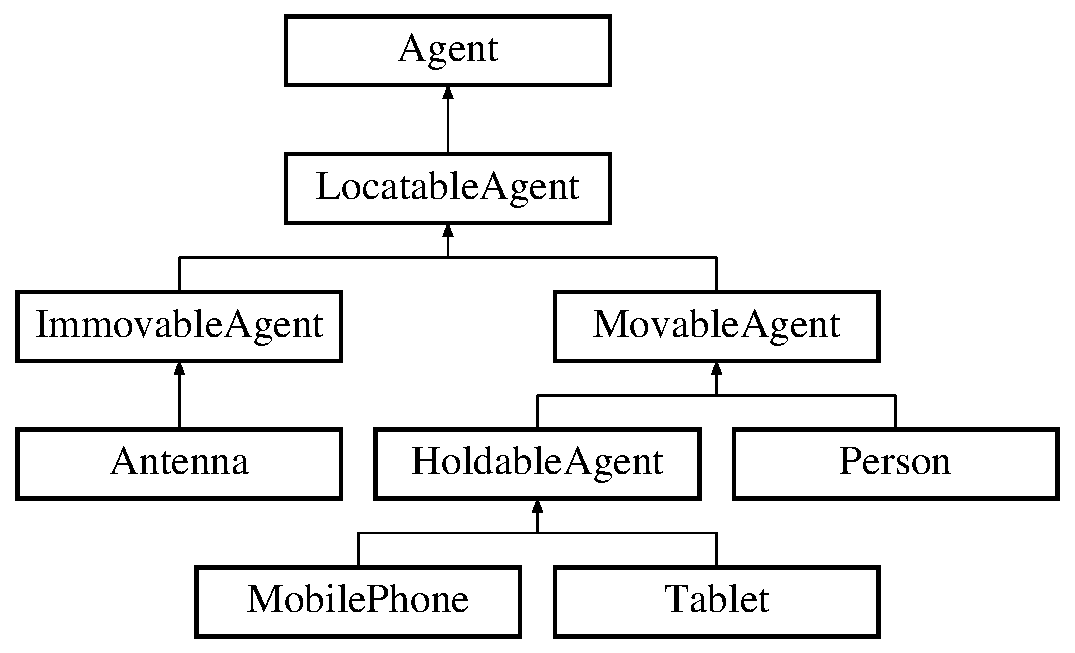
\includegraphics[height=5.000000cm]{class_agent}
\end{center}
\end{figure}
\subsection*{Public Member Functions}
\begin{DoxyCompactItemize}
\item 
\textbf{ Agent} (const \textbf{ Map} $\ast$m, const unsigned long id, const \textbf{ Clock} $\ast$clock)
\item 
virtual \textbf{ $\sim$\+Agent} ()
\item 
bool \textbf{ operator==} (const \textbf{ Agent} \&a)
\item 
virtual const string \textbf{ get\+Name} () const =0
\item 
virtual const string \textbf{ to\+String} () const =0
\item 
const \textbf{ Map} $\ast$ \textbf{ get\+Map} () const
\item 
void \textbf{ set\+Map} (const \textbf{ Map} $\ast$map)
\item 
const \textbf{ Clock} $\ast$ \textbf{ get\+Clock} () const
\item 
const unsigned long \textbf{ get\+Id} () const
\end{DoxyCompactItemize}
\subsection*{Private Attributes}
\begin{DoxyCompactItemize}
\item 
const \textbf{ Map} $\ast$ \textbf{ m\+\_\+map}
\item 
const unsigned long \textbf{ m\+\_\+id}
\item 
const \textbf{ Clock} $\ast$ \textbf{ m\+\_\+clock}
\end{DoxyCompactItemize}


\subsection{Detailed Description}


Definition at line 17 of file Agent.\+h.



\subsection{Constructor \& Destructor Documentation}
\mbox{\label{class_agent_a0ad923f2f9966b65a5d908cb9da4217c}} 
\index{Agent@{Agent}!Agent@{Agent}}
\index{Agent@{Agent}!Agent@{Agent}}
\subsubsection{Agent()}
{\footnotesize\ttfamily Agent\+::\+Agent (\begin{DoxyParamCaption}\item[{const \textbf{ Map} $\ast$}]{m,  }\item[{const unsigned long}]{id,  }\item[{const \textbf{ Clock} $\ast$}]{clock }\end{DoxyParamCaption})}

Constructor of the class. \doxyref{Agent}{p.}{class_agent} is the base class for all agents used in the simulator\+: persons, antennas, devices. \doxyref{Agent}{p.}{class_agent} is an abstract class, the users should build specific subclasses 
\begin{DoxyParams}{Parameters}
{\em m} & -\/ the \doxyref{Map}{p.}{class_map} where the simulation take place. \\
\hline
{\em id} & -\/ the id of this agent, it uniquely identifies the agent \\
\hline
{\em clock} & -\/ the clock used by the simulator, it is the same for all agents \\
\hline
\end{DoxyParams}
\mbox{\label{class_agent_a4feb26df1cf81760a0e411e393c24d4e}} 
\index{Agent@{Agent}!````~Agent@{$\sim$Agent}}
\index{````~Agent@{$\sim$Agent}!Agent@{Agent}}
\subsubsection{$\sim$Agent()}
{\footnotesize\ttfamily virtual Agent\+::$\sim$\+Agent (\begin{DoxyParamCaption}{ }\end{DoxyParamCaption})\hspace{0.3cm}{\ttfamily [virtual]}}

Default destructor of the class. 

\subsection{Member Function Documentation}
\mbox{\label{class_agent_af80a21a067d04788c23d719d07b04038}} 
\index{Agent@{Agent}!getClock@{getClock}}
\index{getClock@{getClock}!Agent@{Agent}}
\subsubsection{getClock()}
{\footnotesize\ttfamily const \textbf{ Clock}$\ast$ Agent\+::get\+Clock (\begin{DoxyParamCaption}{ }\end{DoxyParamCaption}) const}

Returns a pointer to the \doxyref{Clock}{p.}{class_clock} object used for simulation. All Agents use the same \doxyref{Clock}{p.}{class_clock} object for a simulation. \begin{DoxyReturn}{Returns}

\end{DoxyReturn}
\mbox{\label{class_agent_a51d2d781636f524dc151f3da10955613}} 
\index{Agent@{Agent}!getId@{getId}}
\index{getId@{getId}!Agent@{Agent}}
\subsubsection{getId()}
{\footnotesize\ttfamily const unsigned long Agent\+::get\+Id (\begin{DoxyParamCaption}{ }\end{DoxyParamCaption}) const}

Returns the id of the object. \begin{DoxyReturn}{Returns}
the id of the object. 
\end{DoxyReturn}
\mbox{\label{class_agent_ad1870edeea33b059eca75079be2eb002}} 
\index{Agent@{Agent}!getMap@{getMap}}
\index{getMap@{getMap}!Agent@{Agent}}
\subsubsection{getMap()}
{\footnotesize\ttfamily const \textbf{ Map}$\ast$ Agent\+::get\+Map (\begin{DoxyParamCaption}{ }\end{DoxyParamCaption}) const}

Getter that returns a pointer to the map passed to the constructor when the an object was build. \begin{DoxyReturn}{Returns}
a pointer to the \doxyref{Map}{p.}{class_map} object that was passed to the constructor. All agents use the same map for a simulation. 
\end{DoxyReturn}
\mbox{\label{class_agent_afe6c72d91baf9ee4fe77ea1ed7fef3ba}} 
\index{Agent@{Agent}!getName@{getName}}
\index{getName@{getName}!Agent@{Agent}}
\subsubsection{getName()}
{\footnotesize\ttfamily virtual const string Agent\+::get\+Name (\begin{DoxyParamCaption}{ }\end{DoxyParamCaption}) const\hspace{0.3cm}{\ttfamily [pure virtual]}}

This function is used to get the name of the class. It is a pure virtual function, all subclasses implment it and return the actual name of the class. \begin{DoxyReturn}{Returns}
the name of the class. 
\end{DoxyReturn}


Implemented in \textbf{ Holdable\+Agent} \doxyref{}{p.}{class_holdable_agent_ab330bb40de51a957ef8826af629f94a2}, \textbf{ Antenna} \doxyref{}{p.}{class_antenna_a4ad9da1ca9d79f20b331c22b94c57a02}, \textbf{ Person} \doxyref{}{p.}{class_person_aa2a6f8d7f1d94045a03ca578f2ed272c}, \textbf{ Immovable\+Agent} \doxyref{}{p.}{class_immovable_agent_ae8fbccc744f6f806e47dfd242fa67a1c}, \textbf{ Mobile\+Phone} \doxyref{}{p.}{class_mobile_phone_a1eeac3141baafa75ebcf26fc3a0e4068}, \textbf{ Movable\+Agent} \doxyref{}{p.}{class_movable_agent_abcc1218876c39c996f2cb1eba2b96379}, \textbf{ Locatable\+Agent} \doxyref{}{p.}{class_locatable_agent_a754105958bb672744b525538f1584a7b}, and \textbf{ Tablet} \doxyref{}{p.}{class_tablet_adc7196aaee1e9714236b7cd8825d5826}.

\mbox{\label{class_agent_afa2b3a408bb0694aea46fb2bb59bacf7}} 
\index{Agent@{Agent}!operator==@{operator==}}
\index{operator==@{operator==}!Agent@{Agent}}
\subsubsection{operator==()}
{\footnotesize\ttfamily bool Agent\+::operator== (\begin{DoxyParamCaption}\item[{const \textbf{ Agent} \&}]{a }\end{DoxyParamCaption})}

The equal operator for agents. 
\begin{DoxyParams}{Parameters}
{\em a} & the object with which we test the equality \\
\hline
\end{DoxyParams}
\begin{DoxyReturn}{Returns}
true if this object is the equal to a, flase otherwise. Thw objects are considered to be equal if they have the same id. 
\end{DoxyReturn}
\mbox{\label{class_agent_a87a661874cffb03fa9e474e872810260}} 
\index{Agent@{Agent}!setMap@{setMap}}
\index{setMap@{setMap}!Agent@{Agent}}
\subsubsection{setMap()}
{\footnotesize\ttfamily void Agent\+::set\+Map (\begin{DoxyParamCaption}\item[{const \textbf{ Map} $\ast$}]{map }\end{DoxyParamCaption})}

Sets the \doxyref{Map}{p.}{class_map} to be used by this agent during the simulation. It is not advisable to change the map during a simulation. 
\begin{DoxyParams}{Parameters}
{\em map} & pointer to a \doxyref{Map}{p.}{class_map} object. \\
\hline
\end{DoxyParams}
\mbox{\label{class_agent_a44f291596d10c7878b0641d6ec156328}} 
\index{Agent@{Agent}!toString@{toString}}
\index{toString@{toString}!Agent@{Agent}}
\subsubsection{toString()}
{\footnotesize\ttfamily virtual const string Agent\+::to\+String (\begin{DoxyParamCaption}{ }\end{DoxyParamCaption}) const\hspace{0.3cm}{\ttfamily [pure virtual]}}

Builds a string with of the relevant information of the class. It is useful to output on the console or in a file the description of concrete agents. \begin{DoxyReturn}{Returns}
a string representation of the class content. The values of the members are written in this string. 
\end{DoxyReturn}


Implemented in \textbf{ Holdable\+Agent} \doxyref{}{p.}{class_holdable_agent_a2c581226b8994f24b6b2306ae17dbb52}, \textbf{ Antenna} \doxyref{}{p.}{class_antenna_a7fea30e065f49a3cbcee02f60bd033c8}, \textbf{ Person} \doxyref{}{p.}{class_person_a68872538da519d0a04297f43376db27c}, \textbf{ Mobile\+Phone} \doxyref{}{p.}{class_mobile_phone_a2b7e556d12a43e380786ad0eccf3ce04}, \textbf{ Movable\+Agent} \doxyref{}{p.}{class_movable_agent_a1dee2a6bf93f01006fadfb6fba6c9a59}, \textbf{ Locatable\+Agent} \doxyref{}{p.}{class_locatable_agent_a88674f4c8ab9b1b2f3986b226bf4244f}, \textbf{ Immovable\+Agent} \doxyref{}{p.}{class_immovable_agent_a805b0d18035550d902d617a8c7ccc062}, and \textbf{ Tablet} \doxyref{}{p.}{class_tablet_a3fae01e7d526699476221c6a686a4fba}.



\subsection{Member Data Documentation}
\mbox{\label{class_agent_a534f22ebb0573aa1d58d274632e592cf}} 
\index{Agent@{Agent}!m\_clock@{m\_clock}}
\index{m\_clock@{m\_clock}!Agent@{Agent}}
\subsubsection{m\_clock}
{\footnotesize\ttfamily const \textbf{ Clock}$\ast$ Agent\+::m\+\_\+clock\hspace{0.3cm}{\ttfamily [private]}}



Definition at line 80 of file Agent.\+h.

\mbox{\label{class_agent_ad1f52e164c2a829ef4418940567d6e37}} 
\index{Agent@{Agent}!m\_id@{m\_id}}
\index{m\_id@{m\_id}!Agent@{Agent}}
\subsubsection{m\_id}
{\footnotesize\ttfamily const unsigned long Agent\+::m\+\_\+id\hspace{0.3cm}{\ttfamily [private]}}



Definition at line 79 of file Agent.\+h.

\mbox{\label{class_agent_ab24d62bbfc22946d0c72221c8a43f04a}} 
\index{Agent@{Agent}!m\_map@{m\_map}}
\index{m\_map@{m\_map}!Agent@{Agent}}
\subsubsection{m\_map}
{\footnotesize\ttfamily const \textbf{ Map}$\ast$ Agent\+::m\+\_\+map\hspace{0.3cm}{\ttfamily [private]}}



Definition at line 78 of file Agent.\+h.



The documentation for this class was generated from the following file\+:\begin{DoxyCompactItemize}
\item 
include/\textbf{ Agent.\+h}\end{DoxyCompactItemize}

\hypertarget{class_agents_collection}{}\section{Agents\+Collection Class Reference}
\label{class_agents_collection}\index{Agents\+Collection@{Agents\+Collection}}


{\ttfamily \#include $<$Agents\+Collection.\+h$>$}



Collaboration diagram for Agents\+Collection\+:\nopagebreak
\begin{figure}[H]
\begin{center}
\leavevmode
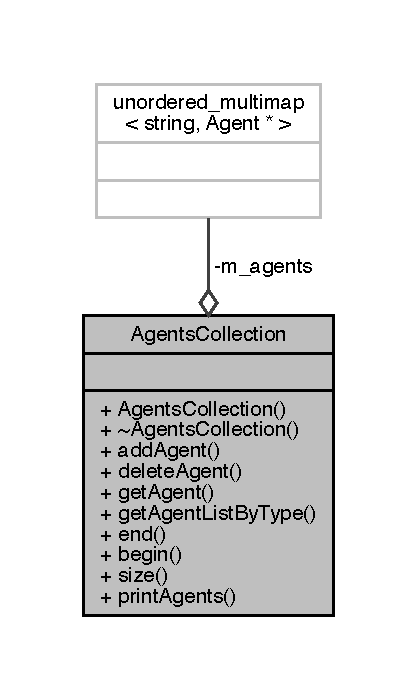
\includegraphics[width=199pt]{class_agents_collection__coll__graph}
\end{center}
\end{figure}
\subsection*{Public Member Functions}
\begin{DoxyCompactItemize}
\item 
\hyperlink{class_agents_collection_a866b0ed56c0109e82bc7c839de0a3267}{Agents\+Collection} ()
\item 
virtual \hyperlink{class_agents_collection_a8a58eb1f8a45cc4d1c0e04dd912dbae0}{$\sim$\+Agents\+Collection} ()
\item 
void \hyperlink{class_agents_collection_a51d14d0635dedd5971ea90dec4f9e7f3}{add\+Agent} (\hyperlink{class_agent}{Agent} $\ast$a)
\item 
\hyperlink{class_agent}{Agent} $\ast$ \hyperlink{class_agents_collection_afd4d2e005b5e449637abd0fa022132a9}{delete\+Agent} (\hyperlink{class_agent}{Agent} $\ast$a)
\item 
\hyperlink{class_agent}{Agent} $\ast$ \hyperlink{class_agents_collection_a4b6b57c50d715edb3404520cfdb32688}{get\+Agent} (const unsigned long id) const
\item 
pair$<$ \hyperlink{_agents_collection_8h_afde47bc45d604b8b8c72755072376679}{um\+\_\+iterator}, \hyperlink{_agents_collection_8h_afde47bc45d604b8b8c72755072376679}{um\+\_\+iterator} $>$ \hyperlink{class_agents_collection_a4ab0c8e86e6f6ebceb12bd2bd8f9f758}{get\+Agent\+List\+By\+Type} (const string \&agent\+Type)
\item 
\hyperlink{_agents_collection_8h_afde47bc45d604b8b8c72755072376679}{um\+\_\+iterator} \hyperlink{class_agents_collection_afc61b751cf3387ab4a1bf0dfbc29cb82}{end} ()
\item 
\hyperlink{_agents_collection_8h_afde47bc45d604b8b8c72755072376679}{um\+\_\+iterator} \hyperlink{class_agents_collection_abc1d6593a3ed1c1c7b2d31b7efec8db8}{begin} ()
\item 
unsigned long \hyperlink{class_agents_collection_a3226f7eb58b11623bdb353d8938f60d3}{size} ()
\item 
void \hyperlink{class_agents_collection_a193faf9793030715e8edeb65137156e9}{print\+Agents} ()
\end{DoxyCompactItemize}
\subsection*{Private Attributes}
\begin{DoxyCompactItemize}
\item 
unordered\+\_\+multimap$<$ string, \hyperlink{class_agent}{Agent} $\ast$ $>$ \hyperlink{class_agents_collection_a35a5728b0e0108c2f37897720c904dd1}{m\+\_\+agents}
\end{DoxyCompactItemize}


\subsection{Detailed Description}
This is actually a container for all the agents used for simulation. An agent could be an object of one the the derived classes of \hyperlink{class_agent}{Agent}. The Agents are kept in an unordered\+\_\+multimap as pairs $<$string, Agent$\ast$$>$ where the first element of the pair is the name of the concrete agent (a person, a mobile device, an antenna, a mno, etc.) and the second element is a pointer to the actual object (agent). 

\subsection{Constructor \& Destructor Documentation}
\mbox{\Hypertarget{class_agents_collection_a866b0ed56c0109e82bc7c839de0a3267}\label{class_agents_collection_a866b0ed56c0109e82bc7c839de0a3267}} 
\index{Agents\+Collection@{Agents\+Collection}!Agents\+Collection@{Agents\+Collection}}
\index{Agents\+Collection@{Agents\+Collection}!Agents\+Collection@{Agents\+Collection}}
\subsubsection{\texorpdfstring{Agents\+Collection()}{AgentsCollection()}}
{\footnotesize\ttfamily Agents\+Collection\+::\+Agents\+Collection (\begin{DoxyParamCaption}{ }\end{DoxyParamCaption})}

The default constructor of the class. \mbox{\Hypertarget{class_agents_collection_a8a58eb1f8a45cc4d1c0e04dd912dbae0}\label{class_agents_collection_a8a58eb1f8a45cc4d1c0e04dd912dbae0}} 
\index{Agents\+Collection@{Agents\+Collection}!````~Agents\+Collection@{$\sim$\+Agents\+Collection}}
\index{````~Agents\+Collection@{$\sim$\+Agents\+Collection}!Agents\+Collection@{Agents\+Collection}}
\subsubsection{\texorpdfstring{$\sim$\+Agents\+Collection()}{~AgentsCollection()}}
{\footnotesize\ttfamily virtual Agents\+Collection\+::$\sim$\+Agents\+Collection (\begin{DoxyParamCaption}{ }\end{DoxyParamCaption})\hspace{0.3cm}{\ttfamily [virtual]}}

Default destructor\+: it iterates through the collection of agents and frees the memory allocated for each agent in the collection. 

\subsection{Member Function Documentation}
\mbox{\Hypertarget{class_agents_collection_a51d14d0635dedd5971ea90dec4f9e7f3}\label{class_agents_collection_a51d14d0635dedd5971ea90dec4f9e7f3}} 
\index{Agents\+Collection@{Agents\+Collection}!add\+Agent@{add\+Agent}}
\index{add\+Agent@{add\+Agent}!Agents\+Collection@{Agents\+Collection}}
\subsubsection{\texorpdfstring{add\+Agent()}{addAgent()}}
{\footnotesize\ttfamily void Agents\+Collection\+::add\+Agent (\begin{DoxyParamCaption}\item[{\hyperlink{class_agent}{Agent} $\ast$}]{a }\end{DoxyParamCaption})}

Adds a new \hyperlink{class_agent}{Agent} to the collection. For performance reasons the \hyperlink{class_agents_collection}{Agents\+Collection} class keep only a pointer to actual agents (objects). 
\begin{DoxyParams}{Parameters}
{\em a} & a pointer to the object (one of the derived classes of the \hyperlink{class_agent}{Agent}) to be added to the collection. \\
\hline
\end{DoxyParams}
\mbox{\Hypertarget{class_agents_collection_abc1d6593a3ed1c1c7b2d31b7efec8db8}\label{class_agents_collection_abc1d6593a3ed1c1c7b2d31b7efec8db8}} 
\index{Agents\+Collection@{Agents\+Collection}!begin@{begin}}
\index{begin@{begin}!Agents\+Collection@{Agents\+Collection}}
\subsubsection{\texorpdfstring{begin()}{begin()}}
{\footnotesize\ttfamily \hyperlink{_agents_collection_8h_afde47bc45d604b8b8c72755072376679}{um\+\_\+iterator} Agents\+Collection\+::begin (\begin{DoxyParamCaption}{ }\end{DoxyParamCaption})}

Iterator to the first agent of the container. \begin{DoxyReturn}{Returns}
a random access iterator pointing to the first element (agent) in the container. If the container is empty, the returned iterator value shall not be dereferenced. 
\end{DoxyReturn}
\mbox{\Hypertarget{class_agents_collection_afd4d2e005b5e449637abd0fa022132a9}\label{class_agents_collection_afd4d2e005b5e449637abd0fa022132a9}} 
\index{Agents\+Collection@{Agents\+Collection}!delete\+Agent@{delete\+Agent}}
\index{delete\+Agent@{delete\+Agent}!Agents\+Collection@{Agents\+Collection}}
\subsubsection{\texorpdfstring{delete\+Agent()}{deleteAgent()}}
{\footnotesize\ttfamily \hyperlink{class_agent}{Agent}$\ast$ Agents\+Collection\+::delete\+Agent (\begin{DoxyParamCaption}\item[{\hyperlink{class_agent}{Agent} $\ast$}]{a }\end{DoxyParamCaption})}

Removes an object from the collection. 
\begin{DoxyParams}{Parameters}
{\em a} & a pointer to the object to be removed from the collection. \\
\hline
\end{DoxyParams}
\begin{DoxyReturn}{Returns}

\end{DoxyReturn}
\mbox{\Hypertarget{class_agents_collection_afc61b751cf3387ab4a1bf0dfbc29cb82}\label{class_agents_collection_afc61b751cf3387ab4a1bf0dfbc29cb82}} 
\index{Agents\+Collection@{Agents\+Collection}!end@{end}}
\index{end@{end}!Agents\+Collection@{Agents\+Collection}}
\subsubsection{\texorpdfstring{end()}{end()}}
{\footnotesize\ttfamily \hyperlink{_agents_collection_8h_afde47bc45d604b8b8c72755072376679}{um\+\_\+iterator} Agents\+Collection\+::end (\begin{DoxyParamCaption}{ }\end{DoxyParamCaption})}

Iterator to the past-\/the-\/end of the collection. It does not point to any agent, and thus shall not be dereferenced. \begin{DoxyReturn}{Returns}
an iterator referring to the past-\/the-\/end element in the agents container. If the container is empty, this function returns the same as Agents\+Colletion\+::begin(). 
\end{DoxyReturn}
\mbox{\Hypertarget{class_agents_collection_a4b6b57c50d715edb3404520cfdb32688}\label{class_agents_collection_a4b6b57c50d715edb3404520cfdb32688}} 
\index{Agents\+Collection@{Agents\+Collection}!get\+Agent@{get\+Agent}}
\index{get\+Agent@{get\+Agent}!Agents\+Collection@{Agents\+Collection}}
\subsubsection{\texorpdfstring{get\+Agent()}{getAgent()}}
{\footnotesize\ttfamily \hyperlink{class_agent}{Agent}$\ast$ Agents\+Collection\+::get\+Agent (\begin{DoxyParamCaption}\item[{const unsigned long}]{id }\end{DoxyParamCaption}) const}

Returns a pointer to an agent from the collection. The agent/object is identified by its id. 
\begin{DoxyParams}{Parameters}
{\em id} & the id of the agent to be returned. \\
\hline
\end{DoxyParams}
\begin{DoxyReturn}{Returns}
a pointer to the agent with the id equal to the parameter id. If there is no agent with the provided id, this method returns nullptr. 
\end{DoxyReturn}
\mbox{\Hypertarget{class_agents_collection_a4ab0c8e86e6f6ebceb12bd2bd8f9f758}\label{class_agents_collection_a4ab0c8e86e6f6ebceb12bd2bd8f9f758}} 
\index{Agents\+Collection@{Agents\+Collection}!get\+Agent\+List\+By\+Type@{get\+Agent\+List\+By\+Type}}
\index{get\+Agent\+List\+By\+Type@{get\+Agent\+List\+By\+Type}!Agents\+Collection@{Agents\+Collection}}
\subsubsection{\texorpdfstring{get\+Agent\+List\+By\+Type()}{getAgentListByType()}}
{\footnotesize\ttfamily pair$<$\hyperlink{_agents_collection_8h_afde47bc45d604b8b8c72755072376679}{um\+\_\+iterator}, \hyperlink{_agents_collection_8h_afde47bc45d604b8b8c72755072376679}{um\+\_\+iterator}$>$ Agents\+Collection\+::get\+Agent\+List\+By\+Type (\begin{DoxyParamCaption}\item[{const string \&}]{agent\+Type }\end{DoxyParamCaption})}

This method is used to get a subset with a certain type of agents\+: persons, mobile phones etc. 
\begin{DoxyParams}{Parameters}
{\em agent\+Type} & is the name of the class of agents that the user wants to retrieve from the collection of all agents. \\
\hline
\end{DoxyParams}
\begin{DoxyReturn}{Returns}
a std\+::pair of iterators of type unordered\+\_\+multimap$<$string, Agent$\ast$$>$\+::iterator that can be used to iterate through to subset of the agents. 
\end{DoxyReturn}
\mbox{\Hypertarget{class_agents_collection_a193faf9793030715e8edeb65137156e9}\label{class_agents_collection_a193faf9793030715e8edeb65137156e9}} 
\index{Agents\+Collection@{Agents\+Collection}!print\+Agents@{print\+Agents}}
\index{print\+Agents@{print\+Agents}!Agents\+Collection@{Agents\+Collection}}
\subsubsection{\texorpdfstring{print\+Agents()}{printAgents()}}
{\footnotesize\ttfamily void Agents\+Collection\+::print\+Agents (\begin{DoxyParamCaption}{ }\end{DoxyParamCaption})}

Print out all agents in the collection. \mbox{\Hypertarget{class_agents_collection_a3226f7eb58b11623bdb353d8938f60d3}\label{class_agents_collection_a3226f7eb58b11623bdb353d8938f60d3}} 
\index{Agents\+Collection@{Agents\+Collection}!size@{size}}
\index{size@{size}!Agents\+Collection@{Agents\+Collection}}
\subsubsection{\texorpdfstring{size()}{size()}}
{\footnotesize\ttfamily unsigned long Agents\+Collection\+::size (\begin{DoxyParamCaption}{ }\end{DoxyParamCaption})}

\begin{DoxyReturn}{Returns}
the number of elements in the container. This is the number of actual objects held in the container, which is not necessarily equal to its storage capacity. 
\end{DoxyReturn}


\subsection{Member Data Documentation}
\mbox{\Hypertarget{class_agents_collection_a35a5728b0e0108c2f37897720c904dd1}\label{class_agents_collection_a35a5728b0e0108c2f37897720c904dd1}} 
\index{Agents\+Collection@{Agents\+Collection}!m\+\_\+agents@{m\+\_\+agents}}
\index{m\+\_\+agents@{m\+\_\+agents}!Agents\+Collection@{Agents\+Collection}}
\subsubsection{\texorpdfstring{m\+\_\+agents}{m\_agents}}
{\footnotesize\ttfamily unordered\+\_\+multimap$<$string, \hyperlink{class_agent}{Agent}$\ast$$>$ Agents\+Collection\+::m\+\_\+agents\hspace{0.3cm}{\ttfamily [private]}}



The documentation for this class was generated from the following file\+:\begin{DoxyCompactItemize}
\item 
include/agent/\hyperlink{_agents_collection_8h}{Agents\+Collection.\+h}\end{DoxyCompactItemize}

\section{Antenna Class Reference}
\label{class_antenna}\index{Antenna@{Antenna}}


{\ttfamily \#include $<$Antenna.\+h$>$}

Inheritance diagram for Antenna\+:\begin{figure}[H]
\begin{center}
\leavevmode
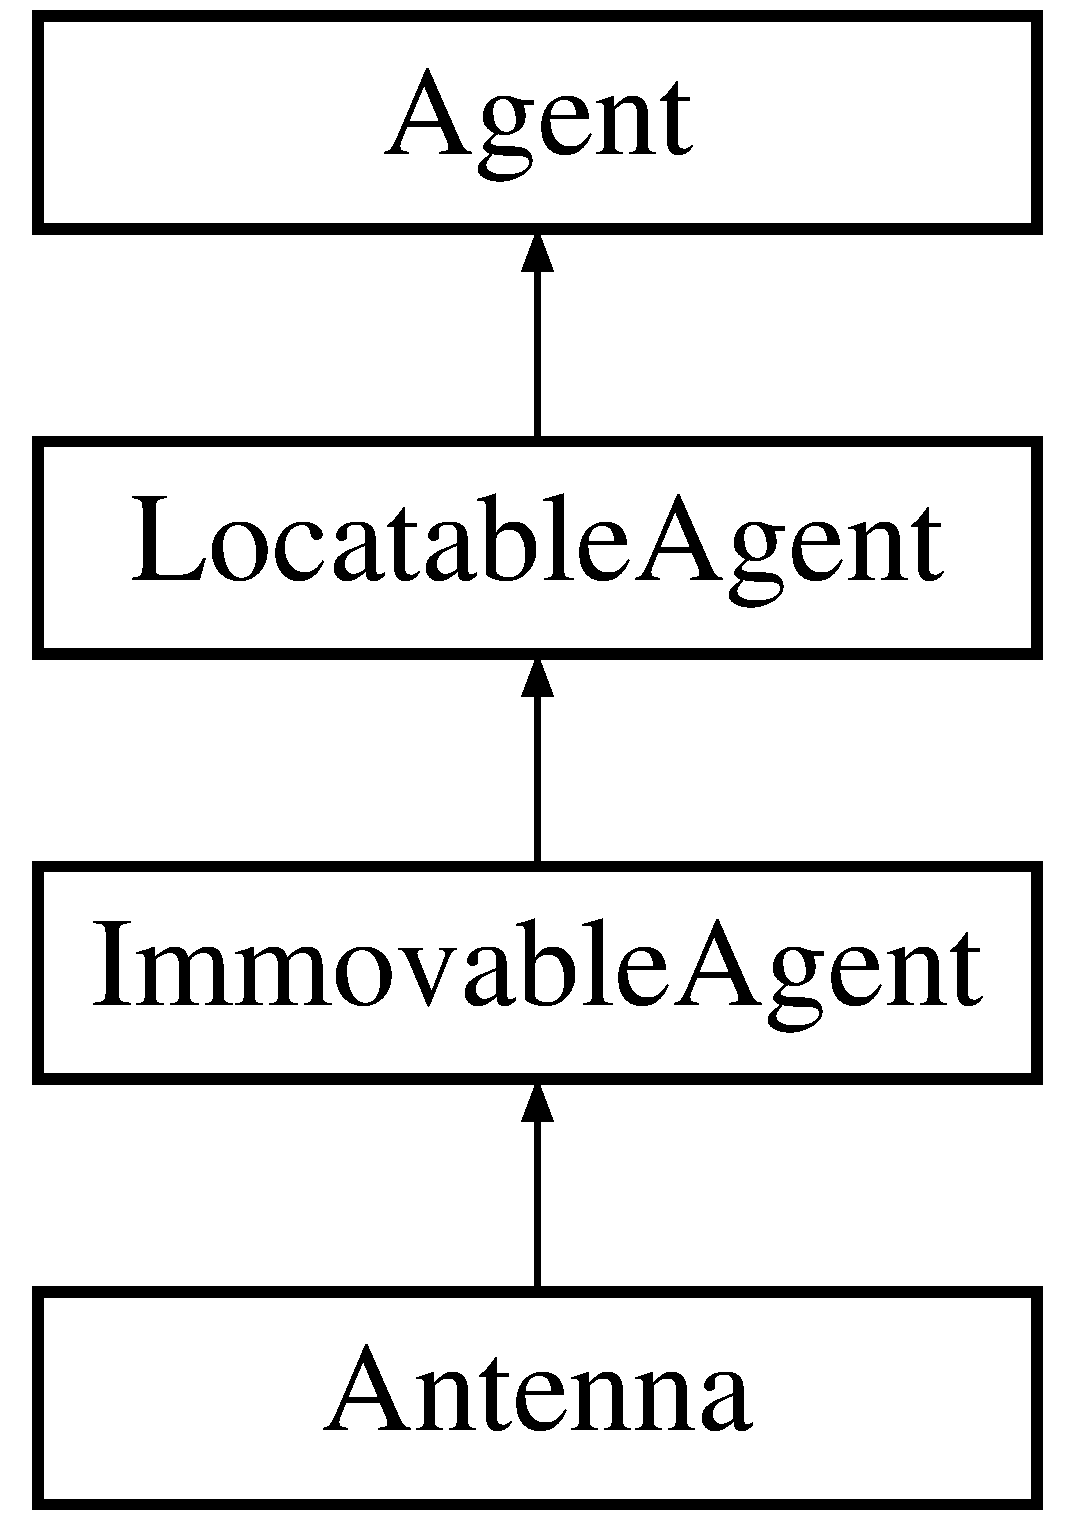
\includegraphics[height=4.000000cm]{class_antenna}
\end{center}
\end{figure}
\subsection*{Public Member Functions}
\begin{DoxyCompactItemize}
\item 
\textbf{ Antenna} (const \textbf{ Map} $\ast$m, const unsigned long id, Point $\ast$init\+Position, const \textbf{ Clock} $\ast$clock, double attenuation\+Factor, double power, unsigned long max\+Connections, double smid, double ssteep, \textbf{ Antenna\+Type} type)
\item 
\textbf{ Antenna} (const \textbf{ Map} $\ast$m, const \textbf{ Clock} $\ast$clock, const unsigned long id, X\+M\+L\+Element $\ast$el)
\item 
virtual \textbf{ $\sim$\+Antenna} ()
\item 
const string \textbf{ get\+Name} () const override
\item 
const string \textbf{ to\+String} () const override
\item 
double \textbf{ get\+Attenuation\+Factor} () const
\item 
void \textbf{ set\+Attenuation\+Factor} (double attenuation\+Factor)
\item 
double \textbf{ get\+Power} () const
\item 
void \textbf{ set\+Power} (double power)
\item 
unsigned long \textbf{ get\+Max\+Connections} () const
\item 
void \textbf{ set\+Max\+Connections} (int max\+Connections)
\item 
bool \textbf{ try\+Register\+Device} (\textbf{ Holdable\+Agent} $\ast$device)
\item 
void \textbf{ attach\+Device} (\textbf{ Holdable\+Agent} $\ast$device)
\item 
void \textbf{ dettach\+Device} (\textbf{ Holdable\+Agent} $\ast$device)
\item 
\textbf{ Antenna\+Type} \textbf{ get\+Type} () const
\item 
void \textbf{ set\+Type} (\textbf{ Antenna\+Type} type)
\item 
double \textbf{ S} (double dist) const
\item 
double \textbf{ get\+Smid} () const
\item 
void \textbf{ set\+Smid} (double smid)
\item 
double \textbf{ get\+S\+Steep} () const
\item 
void \textbf{ set\+S\+Steep} (double s\+Steep)
\item 
double \textbf{ compute\+Signal\+Quality} (const Point $\ast$p) const
\item 
double \textbf{ compute\+Power} (const Point $\ast$p) const
\end{DoxyCompactItemize}
\subsection*{Private Member Functions}
\begin{DoxyCompactItemize}
\item 
bool \textbf{ already\+Registered} (\textbf{ Holdable\+Agent} $\ast$ag)
\item 
void \textbf{ register\+Event} (\textbf{ Holdable\+Agent} $\ast$ag, const \textbf{ Event\+Type} event, const bool verbose)
\item 
unsigned long \textbf{ get\+Num\+Active\+Conections} ()
\item 
double \textbf{ S0} () const
\item 
double \textbf{ S\+Dist} (double dist) const
\end{DoxyCompactItemize}
\subsection*{Private Attributes}
\begin{DoxyCompactItemize}
\item 
double \textbf{ m\+\_\+attenuation\+Factor}
\item 
double \textbf{ m\+\_\+power}
\item 
unsigned long \textbf{ m\+\_\+max\+Connections}
\item 
double \textbf{ m\+\_\+\+Smid}
\item 
double \textbf{ m\+\_\+\+S\+Steep}
\item 
Polygon $\ast$ \textbf{ m\+\_\+cell}
\item 
vector$<$ \textbf{ Holdable\+Agent} $\ast$ $>$ \textbf{ m\+\_\+devices}
\item 
\textbf{ Antenna\+Type} \textbf{ m\+\_\+type}
\item 
ofstream \textbf{ m\+\_\+file}
\end{DoxyCompactItemize}


\subsection{Detailed Description}
This class simulates an antenna of the mobile phone network. 

Definition at line 29 of file Antenna.\+h.



\subsection{Constructor \& Destructor Documentation}
\mbox{\label{class_antenna_a39c505109145908a5b032a16a2fe53c4}} 
\index{Antenna@{Antenna}!Antenna@{Antenna}}
\index{Antenna@{Antenna}!Antenna@{Antenna}}
\subsubsection{Antenna()\hspace{0.1cm}{\footnotesize\ttfamily [1/2]}}
{\footnotesize\ttfamily Antenna\+::\+Antenna (\begin{DoxyParamCaption}\item[{const \textbf{ Map} $\ast$}]{m,  }\item[{const unsigned long}]{id,  }\item[{Point $\ast$}]{init\+Position,  }\item[{const \textbf{ Clock} $\ast$}]{clock,  }\item[{double}]{attenuation\+Factor,  }\item[{double}]{power,  }\item[{unsigned long}]{max\+Connections,  }\item[{double}]{smid,  }\item[{double}]{ssteep,  }\item[{\textbf{ Antenna\+Type}}]{type }\end{DoxyParamCaption})\hspace{0.3cm}{\ttfamily [explicit]}}

Constructor of the class. It builds an object providing directly the values for each parameter of the antenna. 
\begin{DoxyParams}{Parameters}
{\em m} & a pointer to the \doxyref{Map}{p.}{class_map} object used for the simulation \\
\hline
{\em id} & the id of the \doxyref{Antenna}{p.}{class_antenna} \\
\hline
{\em init\+Position} & the position of the antenna on the map \\
\hline
{\em clock} & a pointer to the \doxyref{Clock}{p.}{class_clock} object used for the simulation \\
\hline
{\em attenuation\+Factor} & the attenuation factor of the surrounding environment. In real life, it takes values between 2 (in open field) and 6 (inside buildings). \\
\hline
{\em power} & the power of the antenna in Watts. \\
\hline
{\em max\+Connections} & the maximum number of the connections that the antenna can accept. \\
\hline
{\em smid} & is a parameter of an antenna. The significance of this parameter is described in mobloc R package. \\
\hline
{\em ssteep} & is a parameter of an antenna. The significance of this parameter is described in mobloc R package. \\
\hline
{\em type} & it could have two values \doxyref{Antenna\+Type\+::\+O\+M\+N\+I\+D\+I\+R\+E\+C\+T\+I\+O\+N\+AL}{p.}{_antenna_type_8h_a7b678b5cb9dedc607131200119d96b16a8ff57fa72952e98025e600a041b8b8de} for omnidirectional antennas and \doxyref{Antenna\+Type\+::\+D\+I\+R\+E\+C\+T\+I\+O\+N\+AL}{p.}{_antenna_type_8h_a7b678b5cb9dedc607131200119d96b16ab6f2249394a4def60a78b342dcc925b9} for directional antennas. \\
\hline
\end{DoxyParams}
\mbox{\label{class_antenna_a86c73cfb78910fbaedd6ceb4e226dc9b}} 
\index{Antenna@{Antenna}!Antenna@{Antenna}}
\index{Antenna@{Antenna}!Antenna@{Antenna}}
\subsubsection{Antenna()\hspace{0.1cm}{\footnotesize\ttfamily [2/2]}}
{\footnotesize\ttfamily Antenna\+::\+Antenna (\begin{DoxyParamCaption}\item[{const \textbf{ Map} $\ast$}]{m,  }\item[{const \textbf{ Clock} $\ast$}]{clock,  }\item[{const unsigned long}]{id,  }\item[{X\+M\+L\+Element $\ast$}]{el }\end{DoxyParamCaption})\hspace{0.3cm}{\ttfamily [explicit]}}

Constructor of the class. It builds an object taking the value of the antenna\textquotesingle{} parameters from an X\+ML Element, usually when an \doxyref{Antenna}{p.}{class_antenna} object is built reading the xml configuration file. 
\begin{DoxyParams}{Parameters}
{\em m} & a pointer to the \doxyref{Map}{p.}{class_map} object used for the simulation \\
\hline
{\em clock} & a pointer to the \doxyref{Clock}{p.}{class_clock} object used for the simulation \\
\hline
{\em id} & the id of the \doxyref{Antenna}{p.}{class_antenna} \\
\hline
{\em el} & the X\+ML Element containing the parameters of the \doxyref{Antenna}{p.}{class_antenna}. \\
\hline
\end{DoxyParams}
\mbox{\label{class_antenna_ad7b98073b970db5d6bc83c5c5961fe44}} 
\index{Antenna@{Antenna}!````~Antenna@{$\sim$Antenna}}
\index{````~Antenna@{$\sim$Antenna}!Antenna@{Antenna}}
\subsubsection{$\sim$Antenna()}
{\footnotesize\ttfamily virtual Antenna\+::$\sim$\+Antenna (\begin{DoxyParamCaption}{ }\end{DoxyParamCaption})\hspace{0.3cm}{\ttfamily [virtual]}}

Destructor of the class. It closes the file where the \doxyref{Antenna}{p.}{class_antenna} dumps the registered events during the simulation. 

\subsection{Member Function Documentation}
\mbox{\label{class_antenna_af4fb83843393bf36bdcaefae5b5dd0dd}} 
\index{Antenna@{Antenna}!alreadyRegistered@{alreadyRegistered}}
\index{alreadyRegistered@{alreadyRegistered}!Antenna@{Antenna}}
\subsubsection{alreadyRegistered()}
{\footnotesize\ttfamily bool Antenna\+::already\+Registered (\begin{DoxyParamCaption}\item[{\textbf{ Holdable\+Agent} $\ast$}]{ag }\end{DoxyParamCaption})\hspace{0.3cm}{\ttfamily [private]}}

\mbox{\label{class_antenna_a9c804d991a545157feb066761b6a69ef}} 
\index{Antenna@{Antenna}!attachDevice@{attachDevice}}
\index{attachDevice@{attachDevice}!Antenna@{Antenna}}
\subsubsection{attachDevice()}
{\footnotesize\ttfamily void Antenna\+::attach\+Device (\begin{DoxyParamCaption}\item[{\textbf{ Holdable\+Agent} $\ast$}]{device }\end{DoxyParamCaption})}

Connects a new mobile device and outputs an event \doxyref{Event\+Type\+::\+A\+T\+T\+A\+C\+H\+\_\+\+D\+E\+V\+I\+CE}{p.}{_event_type_8h_a2628ea8d12e8b2563c32f05dc7fff6faa9893a3a649e7100d87b1560bd8202ec2} in the output file. Internally, the antenna keeps a vector with all connected mobile devices. devices. When a new mobile device is connected it is added to this vector. 
\begin{DoxyParams}{Parameters}
{\em device} & a pointer to the object that represents the mobile device connected to this antenna. \\
\hline
\end{DoxyParams}
\mbox{\label{class_antenna_a7caa8004be14f97db64fdf7ae46d6c97}} 
\index{Antenna@{Antenna}!computePower@{computePower}}
\index{computePower@{computePower}!Antenna@{Antenna}}
\subsubsection{computePower()}
{\footnotesize\ttfamily double Antenna\+::compute\+Power (\begin{DoxyParamCaption}\item[{const Point $\ast$}]{p }\end{DoxyParamCaption}) const}

Computes the power of the signal given by an antenna in a certain location. 
\begin{DoxyParams}{Parameters}
{\em p} & the location where we want to compute the power of the signal. \\
\hline
\end{DoxyParams}
\begin{DoxyReturn}{Returns}
the power of the signal in the location given by Point p. 
\end{DoxyReturn}
\mbox{\label{class_antenna_afb03d417efec2423a1b67df16d6ebcb6}} 
\index{Antenna@{Antenna}!computeSignalQuality@{computeSignalQuality}}
\index{computeSignalQuality@{computeSignalQuality}!Antenna@{Antenna}}
\subsubsection{computeSignalQuality()}
{\footnotesize\ttfamily double Antenna\+::compute\+Signal\+Quality (\begin{DoxyParamCaption}\item[{const Point $\ast$}]{p }\end{DoxyParamCaption}) const}

Computes the signal quality given by an antenna in a certain location. 
\begin{DoxyParams}{Parameters}
{\em p} & the location where we want to compute the signal quality. \\
\hline
\end{DoxyParams}
\begin{DoxyReturn}{Returns}
the signal quality. 
\end{DoxyReturn}
\mbox{\label{class_antenna_a983a0784315567c2ab6ac1820cf558c5}} 
\index{Antenna@{Antenna}!dettachDevice@{dettachDevice}}
\index{dettachDevice@{dettachDevice}!Antenna@{Antenna}}
\subsubsection{dettachDevice()}
{\footnotesize\ttfamily void Antenna\+::dettach\+Device (\begin{DoxyParamCaption}\item[{\textbf{ Holdable\+Agent} $\ast$}]{device }\end{DoxyParamCaption})}

Disconnects a mobile device from the antenna and outputs an event Event\+Type\+::\+D\+E\+A\+T\+A\+C\+H\+\_\+\+D\+E\+V\+I\+CE in the output file. Internally, the mobile device is removed from the vector of the connected mobile devices. 
\begin{DoxyParams}{Parameters}
{\em device} & \\
\hline
\end{DoxyParams}
\mbox{\label{class_antenna_a9551ed22d25c51210913de4a3074d9eb}} 
\index{Antenna@{Antenna}!getAttenuationFactor@{getAttenuationFactor}}
\index{getAttenuationFactor@{getAttenuationFactor}!Antenna@{Antenna}}
\subsubsection{getAttenuationFactor()}
{\footnotesize\ttfamily double Antenna\+::get\+Attenuation\+Factor (\begin{DoxyParamCaption}{ }\end{DoxyParamCaption}) const}

Returns the surrounding environment\textquotesingle{} attenuation factor of the signal. \begin{DoxyReturn}{Returns}
the signals\textquotesingle{} attenuation factor of the surrounding environment. In real life, it takes values between 2 (in open field) and 6 (inside buildings). 
\end{DoxyReturn}
\mbox{\label{class_antenna_ac7d42215283cd7d4dc16d449f61af91d}} 
\index{Antenna@{Antenna}!getMaxConnections@{getMaxConnections}}
\index{getMaxConnections@{getMaxConnections}!Antenna@{Antenna}}
\subsubsection{getMaxConnections()}
{\footnotesize\ttfamily unsigned long Antenna\+::get\+Max\+Connections (\begin{DoxyParamCaption}{ }\end{DoxyParamCaption}) const}

Returns the maximum number of mobile devices that an antenna can connect. \mbox{\label{class_antenna_a4ad9da1ca9d79f20b331c22b94c57a02}} 
\index{Antenna@{Antenna}!getName@{getName}}
\index{getName@{getName}!Antenna@{Antenna}}
\subsubsection{getName()}
{\footnotesize\ttfamily const string Antenna\+::get\+Name (\begin{DoxyParamCaption}{ }\end{DoxyParamCaption}) const\hspace{0.3cm}{\ttfamily [override]}, {\ttfamily [virtual]}}

Overrides the same method from the superclass. \begin{DoxyReturn}{Returns}
the name of the class, i.\+e. \char`\"{}\+Antenna\char`\"{} 
\end{DoxyReturn}


Implements \textbf{ Agent} \doxyref{}{p.}{class_agent_afe6c72d91baf9ee4fe77ea1ed7fef3ba}.

\mbox{\label{class_antenna_a86c5c094ab6ea432609afa00f3a8080a}} 
\index{Antenna@{Antenna}!getNumActiveConections@{getNumActiveConections}}
\index{getNumActiveConections@{getNumActiveConections}!Antenna@{Antenna}}
\subsubsection{getNumActiveConections()}
{\footnotesize\ttfamily unsigned long Antenna\+::get\+Num\+Active\+Conections (\begin{DoxyParamCaption}{ }\end{DoxyParamCaption})\hspace{0.3cm}{\ttfamily [private]}}

\mbox{\label{class_antenna_afca01d00c8e393ee911f1e9240b51d2e}} 
\index{Antenna@{Antenna}!getPower@{getPower}}
\index{getPower@{getPower}!Antenna@{Antenna}}
\subsubsection{getPower()}
{\footnotesize\ttfamily double Antenna\+::get\+Power (\begin{DoxyParamCaption}{ }\end{DoxyParamCaption}) const}

Returns the power of an antenna in Watts at the location of antenna. This power decreases with a power of the distance from antenna. \begin{DoxyReturn}{Returns}
the power of an antenna in Watts. 
\end{DoxyReturn}
\mbox{\label{class_antenna_acfaf47d35cc742e76522ea31a8b01578}} 
\index{Antenna@{Antenna}!getSmid@{getSmid}}
\index{getSmid@{getSmid}!Antenna@{Antenna}}
\subsubsection{getSmid()}
{\footnotesize\ttfamily double Antenna\+::get\+Smid (\begin{DoxyParamCaption}{ }\end{DoxyParamCaption}) const}

Returns the value of the Smid antenna parameter. \begin{DoxyReturn}{Returns}
the value of the Smid antenna parameter. 
\end{DoxyReturn}
\mbox{\label{class_antenna_a096deca0fe8497c0fe53539ae80f2db5}} 
\index{Antenna@{Antenna}!getSSteep@{getSSteep}}
\index{getSSteep@{getSSteep}!Antenna@{Antenna}}
\subsubsection{getSSteep()}
{\footnotesize\ttfamily double Antenna\+::get\+S\+Steep (\begin{DoxyParamCaption}{ }\end{DoxyParamCaption}) const}

Returns the value of the Ssteep antenna parameter. \begin{DoxyReturn}{Returns}
the value of the Ssteep antenna parameter. 
\end{DoxyReturn}
\mbox{\label{class_antenna_adf45a8b339956741bf8dcb5361f5f249}} 
\index{Antenna@{Antenna}!getType@{getType}}
\index{getType@{getType}!Antenna@{Antenna}}
\subsubsection{getType()}
{\footnotesize\ttfamily \textbf{ Antenna\+Type} Antenna\+::get\+Type (\begin{DoxyParamCaption}{ }\end{DoxyParamCaption}) const}

Returns the antenna type\+: omnidirectional or directional \begin{DoxyReturn}{Returns}
the antenna type \+: \doxyref{Antenna\+Type\+::\+O\+M\+N\+I\+D\+I\+R\+E\+C\+T\+I\+O\+N\+AL}{p.}{_antenna_type_8h_a7b678b5cb9dedc607131200119d96b16a8ff57fa72952e98025e600a041b8b8de} or \doxyref{Antenna\+Type\+::\+D\+I\+R\+E\+C\+T\+I\+O\+N\+AL}{p.}{_antenna_type_8h_a7b678b5cb9dedc607131200119d96b16ab6f2249394a4def60a78b342dcc925b9}. 
\end{DoxyReturn}
\mbox{\label{class_antenna_aa21a4c0d581c59c36480d932584c0ef5}} 
\index{Antenna@{Antenna}!registerEvent@{registerEvent}}
\index{registerEvent@{registerEvent}!Antenna@{Antenna}}
\subsubsection{registerEvent()}
{\footnotesize\ttfamily void Antenna\+::register\+Event (\begin{DoxyParamCaption}\item[{\textbf{ Holdable\+Agent} $\ast$}]{ag,  }\item[{const \textbf{ Event\+Type}}]{event,  }\item[{const bool}]{verbose }\end{DoxyParamCaption})\hspace{0.3cm}{\ttfamily [private]}}

\mbox{\label{class_antenna_a5715c4100035c58d63b7c9a0195748fe}} 
\index{Antenna@{Antenna}!S@{S}}
\index{S@{S}!Antenna@{Antenna}}
\subsubsection{S()}
{\footnotesize\ttfamily double Antenna\+::S (\begin{DoxyParamCaption}\item[{double}]{dist }\end{DoxyParamCaption}) const}

Computes the signal strength at the distance dist from antenna location. 
\begin{DoxyParams}{Parameters}
{\em dist} & the distance from antenna location. \\
\hline
\end{DoxyParams}
\begin{DoxyReturn}{Returns}
the signal strength. 
\end{DoxyReturn}
\mbox{\label{class_antenna_a033246c50bec80123860154a949620c7}} 
\index{Antenna@{Antenna}!S0@{S0}}
\index{S0@{S0}!Antenna@{Antenna}}
\subsubsection{S0()}
{\footnotesize\ttfamily double Antenna\+::\+S0 (\begin{DoxyParamCaption}{ }\end{DoxyParamCaption}) const\hspace{0.3cm}{\ttfamily [private]}}

\mbox{\label{class_antenna_ae60ab40ded94be407c3b7455f4e886fe}} 
\index{Antenna@{Antenna}!SDist@{SDist}}
\index{SDist@{SDist}!Antenna@{Antenna}}
\subsubsection{SDist()}
{\footnotesize\ttfamily double Antenna\+::\+S\+Dist (\begin{DoxyParamCaption}\item[{double}]{dist }\end{DoxyParamCaption}) const\hspace{0.3cm}{\ttfamily [private]}}

\mbox{\label{class_antenna_a8697756860ff821a92e9404e00a55f89}} 
\index{Antenna@{Antenna}!setAttenuationFactor@{setAttenuationFactor}}
\index{setAttenuationFactor@{setAttenuationFactor}!Antenna@{Antenna}}
\subsubsection{setAttenuationFactor()}
{\footnotesize\ttfamily void Antenna\+::set\+Attenuation\+Factor (\begin{DoxyParamCaption}\item[{double}]{attenuation\+Factor }\end{DoxyParamCaption})}

Sets the surrounding environment\textquotesingle{} attenuation factor of the signal for an antenna. 
\begin{DoxyParams}{Parameters}
{\em attenuation\+Factor} & the value of the surrounding environment\textquotesingle{} attenuation factor of the signal. In real life, it takes values between 2 (in open field) and 6 (inside buildings). \\
\hline
\end{DoxyParams}
\mbox{\label{class_antenna_ad844ed8507afb83b74b804c2434a4e50}} 
\index{Antenna@{Antenna}!setMaxConnections@{setMaxConnections}}
\index{setMaxConnections@{setMaxConnections}!Antenna@{Antenna}}
\subsubsection{setMaxConnections()}
{\footnotesize\ttfamily void Antenna\+::set\+Max\+Connections (\begin{DoxyParamCaption}\item[{int}]{max\+Connections }\end{DoxyParamCaption})}

Sets the number of mobile devices that an antenna can connect. 
\begin{DoxyParams}{Parameters}
{\em max\+Connections} & the number of mobile devices that an antenna can connect. \\
\hline
\end{DoxyParams}
\mbox{\label{class_antenna_a172a4c7765dea045d6504f6e2cbe0f59}} 
\index{Antenna@{Antenna}!setPower@{setPower}}
\index{setPower@{setPower}!Antenna@{Antenna}}
\subsubsection{setPower()}
{\footnotesize\ttfamily void Antenna\+::set\+Power (\begin{DoxyParamCaption}\item[{double}]{power }\end{DoxyParamCaption})}

Sets the power of an antenna. 
\begin{DoxyParams}{Parameters}
{\em power} & the value of the antenna\textquotesingle{}s power. \\
\hline
\end{DoxyParams}
\mbox{\label{class_antenna_a67e5ae0106189d18e4f114d8e0e14a09}} 
\index{Antenna@{Antenna}!setSmid@{setSmid}}
\index{setSmid@{setSmid}!Antenna@{Antenna}}
\subsubsection{setSmid()}
{\footnotesize\ttfamily void Antenna\+::set\+Smid (\begin{DoxyParamCaption}\item[{double}]{smid }\end{DoxyParamCaption})}

Sets the value of the Smid antenna parameter. 
\begin{DoxyParams}{Parameters}
{\em smid} & the value of the Smid antenna parameter. \\
\hline
\end{DoxyParams}
\mbox{\label{class_antenna_a92357bee36ba7dcfd08c4d2ce2280e3c}} 
\index{Antenna@{Antenna}!setSSteep@{setSSteep}}
\index{setSSteep@{setSSteep}!Antenna@{Antenna}}
\subsubsection{setSSteep()}
{\footnotesize\ttfamily void Antenna\+::set\+S\+Steep (\begin{DoxyParamCaption}\item[{double}]{s\+Steep }\end{DoxyParamCaption})}

Sets the value of the Ssteep antenna parameter. 
\begin{DoxyParams}{Parameters}
{\em s\+Steep} & the value of the Ssteep antenna parameter. \\
\hline
\end{DoxyParams}
\mbox{\label{class_antenna_aa9a8414c469e6dd49eed7a7cc58725c1}} 
\index{Antenna@{Antenna}!setType@{setType}}
\index{setType@{setType}!Antenna@{Antenna}}
\subsubsection{setType()}
{\footnotesize\ttfamily void Antenna\+::set\+Type (\begin{DoxyParamCaption}\item[{\textbf{ Antenna\+Type}}]{type }\end{DoxyParamCaption})}

Sets the antenna type. 
\begin{DoxyParams}{Parameters}
{\em type} & the antenna type. It could take the following two values\+: \doxyref{Antenna\+Type\+::\+O\+M\+N\+I\+D\+I\+R\+E\+C\+T\+I\+O\+N\+AL}{p.}{_antenna_type_8h_a7b678b5cb9dedc607131200119d96b16a8ff57fa72952e98025e600a041b8b8de} or \doxyref{Antenna\+Type\+::\+D\+I\+R\+E\+C\+T\+I\+O\+N\+AL}{p.}{_antenna_type_8h_a7b678b5cb9dedc607131200119d96b16ab6f2249394a4def60a78b342dcc925b9}. \\
\hline
\end{DoxyParams}
\mbox{\label{class_antenna_a7fea30e065f49a3cbcee02f60bd033c8}} 
\index{Antenna@{Antenna}!toString@{toString}}
\index{toString@{toString}!Antenna@{Antenna}}
\subsubsection{toString()}
{\footnotesize\ttfamily const string Antenna\+::to\+String (\begin{DoxyParamCaption}{ }\end{DoxyParamCaption}) const\hspace{0.3cm}{\ttfamily [override]}, {\ttfamily [virtual]}}

Overrides the same method from the superclass. It is used to write the characteristics of the \doxyref{Antenna}{p.}{class_antenna} in a file or console. \begin{DoxyReturn}{Returns}
a string that describes the parameters of the \doxyref{Antenna}{p.}{class_antenna}. 
\end{DoxyReturn}


Implements \textbf{ Agent} \doxyref{}{p.}{class_agent_a44f291596d10c7878b0641d6ec156328}.

\mbox{\label{class_antenna_a4455f5c804e1ea520dd849dc9fd7b0b4}} 
\index{Antenna@{Antenna}!tryRegisterDevice@{tryRegisterDevice}}
\index{tryRegisterDevice@{tryRegisterDevice}!Antenna@{Antenna}}
\subsubsection{tryRegisterDevice()}
{\footnotesize\ttfamily bool Antenna\+::try\+Register\+Device (\begin{DoxyParamCaption}\item[{\textbf{ Holdable\+Agent} $\ast$}]{device }\end{DoxyParamCaption})}

Tries to register a mobile device as being connected to this antenna. 
\begin{DoxyParams}{Parameters}
{\em device} & a pointer to the object that represents a mobile device. \\
\hline
\end{DoxyParams}
\begin{DoxyReturn}{Returns}
true if the connection is successful, false otherwise. 
\end{DoxyReturn}


\subsection{Member Data Documentation}
\mbox{\label{class_antenna_a77728d7c2315dda0ebc42235ae0bdf0a}} 
\index{Antenna@{Antenna}!m\_attenuationFactor@{m\_attenuationFactor}}
\index{m\_attenuationFactor@{m\_attenuationFactor}!Antenna@{Antenna}}
\subsubsection{m\_attenuationFactor}
{\footnotesize\ttfamily double Antenna\+::m\+\_\+attenuation\+Factor\hspace{0.3cm}{\ttfamily [private]}}



Definition at line 207 of file Antenna.\+h.

\mbox{\label{class_antenna_a185c9c47cb6d528622510af50c5ff62a}} 
\index{Antenna@{Antenna}!m\_cell@{m\_cell}}
\index{m\_cell@{m\_cell}!Antenna@{Antenna}}
\subsubsection{m\_cell}
{\footnotesize\ttfamily Polygon$\ast$ Antenna\+::m\+\_\+cell\hspace{0.3cm}{\ttfamily [private]}}



Definition at line 213 of file Antenna.\+h.

\mbox{\label{class_antenna_a2d0f7032eb1d8cc6c02b1dd64bc59856}} 
\index{Antenna@{Antenna}!m\_devices@{m\_devices}}
\index{m\_devices@{m\_devices}!Antenna@{Antenna}}
\subsubsection{m\_devices}
{\footnotesize\ttfamily vector$<$\textbf{ Holdable\+Agent}$\ast$$>$ Antenna\+::m\+\_\+devices\hspace{0.3cm}{\ttfamily [private]}}



Definition at line 214 of file Antenna.\+h.

\mbox{\label{class_antenna_a06824840191e96b19eb224d53e08d3ec}} 
\index{Antenna@{Antenna}!m\_file@{m\_file}}
\index{m\_file@{m\_file}!Antenna@{Antenna}}
\subsubsection{m\_file}
{\footnotesize\ttfamily ofstream Antenna\+::m\+\_\+file\hspace{0.3cm}{\ttfamily [private]}}



Definition at line 216 of file Antenna.\+h.

\mbox{\label{class_antenna_a06480ddd6e9a9cb4d88c4cea72e2d2ab}} 
\index{Antenna@{Antenna}!m\_maxConnections@{m\_maxConnections}}
\index{m\_maxConnections@{m\_maxConnections}!Antenna@{Antenna}}
\subsubsection{m\_maxConnections}
{\footnotesize\ttfamily unsigned long Antenna\+::m\+\_\+max\+Connections\hspace{0.3cm}{\ttfamily [private]}}



Definition at line 209 of file Antenna.\+h.

\mbox{\label{class_antenna_a89874a2fbd083c99f780482bf4642b07}} 
\index{Antenna@{Antenna}!m\_power@{m\_power}}
\index{m\_power@{m\_power}!Antenna@{Antenna}}
\subsubsection{m\_power}
{\footnotesize\ttfamily double Antenna\+::m\+\_\+power\hspace{0.3cm}{\ttfamily [private]}}



Definition at line 208 of file Antenna.\+h.

\mbox{\label{class_antenna_ae5f536b16d9d924a7ee7cba954c44d05}} 
\index{Antenna@{Antenna}!m\_Smid@{m\_Smid}}
\index{m\_Smid@{m\_Smid}!Antenna@{Antenna}}
\subsubsection{m\_Smid}
{\footnotesize\ttfamily double Antenna\+::m\+\_\+\+Smid\hspace{0.3cm}{\ttfamily [private]}}



Definition at line 210 of file Antenna.\+h.

\mbox{\label{class_antenna_a48117d47d70c758f5a09c54fa323feed}} 
\index{Antenna@{Antenna}!m\_SSteep@{m\_SSteep}}
\index{m\_SSteep@{m\_SSteep}!Antenna@{Antenna}}
\subsubsection{m\_SSteep}
{\footnotesize\ttfamily double Antenna\+::m\+\_\+\+S\+Steep\hspace{0.3cm}{\ttfamily [private]}}



Definition at line 211 of file Antenna.\+h.

\mbox{\label{class_antenna_a6b68373c8b139e8dafc4c11480eee0e1}} 
\index{Antenna@{Antenna}!m\_type@{m\_type}}
\index{m\_type@{m\_type}!Antenna@{Antenna}}
\subsubsection{m\_type}
{\footnotesize\ttfamily \textbf{ Antenna\+Type} Antenna\+::m\+\_\+type\hspace{0.3cm}{\ttfamily [private]}}



Definition at line 215 of file Antenna.\+h.



The documentation for this class was generated from the following file\+:\begin{DoxyCompactItemize}
\item 
include/\textbf{ Antenna.\+h}\end{DoxyCompactItemize}

\section{Antenna\+Info Class Reference}
\label{class_antenna_info}\index{AntennaInfo@{AntennaInfo}}


{\ttfamily \#include $<$Antenna\+Info.\+h$>$}

\subsection*{Public Member Functions}
\begin{DoxyCompactItemize}
\item 
\textbf{ Antenna\+Info} (unsigned long time, unsigned long antenna\+Id, unsigned long event, unsigned long device\+Id, double x, double y)
\item 
unsigned long \textbf{ get\+Antenna\+Id} () const
\item 
unsigned long \textbf{ get\+Device\+Id} () const
\item 
unsigned long \textbf{ get\+Event\+Code} () const
\item 
unsigned long \textbf{ get\+Time} () const
\item 
double \textbf{ getX} () const
\item 
double \textbf{ getY} () const
\item 
string \textbf{ to\+String} () const
\end{DoxyCompactItemize}
\subsection*{Private Attributes}
\begin{DoxyCompactItemize}
\item 
unsigned long \textbf{ m\+\_\+time}
\item 
unsigned long \textbf{ m\+\_\+antenna\+Id}
\item 
unsigned long \textbf{ m\+\_\+event\+Code}
\item 
unsigned long \textbf{ m\+\_\+device\+Id}
\item 
double \textbf{ m\+\_\+x}
\item 
double \textbf{ m\+\_\+y}
\end{DoxyCompactItemize}


\subsection{Detailed Description}


Definition at line 19 of file Antenna\+Info.\+h.



\subsection{Constructor \& Destructor Documentation}
\mbox{\label{class_antenna_info_a3844c960562688818ed9d9cb2bde82d7}} 
\index{AntennaInfo@{AntennaInfo}!AntennaInfo@{AntennaInfo}}
\index{AntennaInfo@{AntennaInfo}!AntennaInfo@{AntennaInfo}}
\subsubsection{AntennaInfo()}
{\footnotesize\ttfamily Antenna\+Info\+::\+Antenna\+Info (\begin{DoxyParamCaption}\item[{unsigned long}]{time,  }\item[{unsigned long}]{antenna\+Id,  }\item[{unsigned long}]{event,  }\item[{unsigned long}]{device\+Id,  }\item[{double}]{x,  }\item[{double}]{y }\end{DoxyParamCaption})}



Definition at line 16 of file Antenna\+Info.\+cpp.



\subsection{Member Function Documentation}
\mbox{\label{class_antenna_info_a1aee619b1f3d45e3da945f17d8531bbf}} 
\index{AntennaInfo@{AntennaInfo}!getAntennaId@{getAntennaId}}
\index{getAntennaId@{getAntennaId}!AntennaInfo@{AntennaInfo}}
\subsubsection{getAntennaId()}
{\footnotesize\ttfamily unsigned long Antenna\+Info\+::get\+Antenna\+Id (\begin{DoxyParamCaption}{ }\end{DoxyParamCaption}) const}



Definition at line 22 of file Antenna\+Info.\+cpp.



References m\+\_\+antenna\+Id.

\mbox{\label{class_antenna_info_a25a6a3ca6afeba45c00f2312b8d2d9de}} 
\index{AntennaInfo@{AntennaInfo}!getDeviceId@{getDeviceId}}
\index{getDeviceId@{getDeviceId}!AntennaInfo@{AntennaInfo}}
\subsubsection{getDeviceId()}
{\footnotesize\ttfamily unsigned long Antenna\+Info\+::get\+Device\+Id (\begin{DoxyParamCaption}{ }\end{DoxyParamCaption}) const}



Definition at line 26 of file Antenna\+Info.\+cpp.



References m\+\_\+device\+Id.

\mbox{\label{class_antenna_info_a898d46ed6fd2676e370ae8c325ffd679}} 
\index{AntennaInfo@{AntennaInfo}!getEventCode@{getEventCode}}
\index{getEventCode@{getEventCode}!AntennaInfo@{AntennaInfo}}
\subsubsection{getEventCode()}
{\footnotesize\ttfamily unsigned long Antenna\+Info\+::get\+Event\+Code (\begin{DoxyParamCaption}{ }\end{DoxyParamCaption}) const}



Definition at line 30 of file Antenna\+Info.\+cpp.



References m\+\_\+event\+Code.

\mbox{\label{class_antenna_info_aaae1e1105ba4a724c0061e3f7904b1e5}} 
\index{AntennaInfo@{AntennaInfo}!getTime@{getTime}}
\index{getTime@{getTime}!AntennaInfo@{AntennaInfo}}
\subsubsection{getTime()}
{\footnotesize\ttfamily unsigned long Antenna\+Info\+::get\+Time (\begin{DoxyParamCaption}{ }\end{DoxyParamCaption}) const}



Definition at line 34 of file Antenna\+Info.\+cpp.



References m\+\_\+time.

\mbox{\label{class_antenna_info_a3817cba0231888dc5977105ace0faddb}} 
\index{AntennaInfo@{AntennaInfo}!getX@{getX}}
\index{getX@{getX}!AntennaInfo@{AntennaInfo}}
\subsubsection{getX()}
{\footnotesize\ttfamily double Antenna\+Info\+::getX (\begin{DoxyParamCaption}{ }\end{DoxyParamCaption}) const}



Definition at line 38 of file Antenna\+Info.\+cpp.



References m\+\_\+x.

\mbox{\label{class_antenna_info_aa385e3e85d783b81d69014a64b5fc94f}} 
\index{AntennaInfo@{AntennaInfo}!getY@{getY}}
\index{getY@{getY}!AntennaInfo@{AntennaInfo}}
\subsubsection{getY()}
{\footnotesize\ttfamily double Antenna\+Info\+::getY (\begin{DoxyParamCaption}{ }\end{DoxyParamCaption}) const}



Definition at line 42 of file Antenna\+Info.\+cpp.



References m\+\_\+y.

\mbox{\label{class_antenna_info_ab8c9e530f1a7adeb9ca4bb6bc4c4af1a}} 
\index{AntennaInfo@{AntennaInfo}!toString@{toString}}
\index{toString@{toString}!AntennaInfo@{AntennaInfo}}
\subsubsection{toString()}
{\footnotesize\ttfamily string Antenna\+Info\+::to\+String (\begin{DoxyParamCaption}{ }\end{DoxyParamCaption}) const}



Definition at line 46 of file Antenna\+Info.\+cpp.



References m\+\_\+antenna\+Id, m\+\_\+device\+Id, m\+\_\+event\+Code, m\+\_\+time, m\+\_\+x, and m\+\_\+y.



\subsection{Member Data Documentation}
\mbox{\label{class_antenna_info_a7776748da0e4d9f4b39683066806a897}} 
\index{AntennaInfo@{AntennaInfo}!m\_antennaId@{m\_antennaId}}
\index{m\_antennaId@{m\_antennaId}!AntennaInfo@{AntennaInfo}}
\subsubsection{m\_antennaId}
{\footnotesize\ttfamily unsigned long Antenna\+Info\+::m\+\_\+antenna\+Id\hspace{0.3cm}{\ttfamily [private]}}



Definition at line 32 of file Antenna\+Info.\+h.



Referenced by get\+Antenna\+Id(), and to\+String().

\mbox{\label{class_antenna_info_a006ef0511686a6874503ff398b6bf7e8}} 
\index{AntennaInfo@{AntennaInfo}!m\_deviceId@{m\_deviceId}}
\index{m\_deviceId@{m\_deviceId}!AntennaInfo@{AntennaInfo}}
\subsubsection{m\_deviceId}
{\footnotesize\ttfamily unsigned long Antenna\+Info\+::m\+\_\+device\+Id\hspace{0.3cm}{\ttfamily [private]}}



Definition at line 34 of file Antenna\+Info.\+h.



Referenced by get\+Device\+Id(), and to\+String().

\mbox{\label{class_antenna_info_a90e054e1eb790e6b0096bf35a27bbd8e}} 
\index{AntennaInfo@{AntennaInfo}!m\_eventCode@{m\_eventCode}}
\index{m\_eventCode@{m\_eventCode}!AntennaInfo@{AntennaInfo}}
\subsubsection{m\_eventCode}
{\footnotesize\ttfamily unsigned long Antenna\+Info\+::m\+\_\+event\+Code\hspace{0.3cm}{\ttfamily [private]}}



Definition at line 33 of file Antenna\+Info.\+h.



Referenced by get\+Event\+Code(), and to\+String().

\mbox{\label{class_antenna_info_a355d929c83040e154f635ce149286b05}} 
\index{AntennaInfo@{AntennaInfo}!m\_time@{m\_time}}
\index{m\_time@{m\_time}!AntennaInfo@{AntennaInfo}}
\subsubsection{m\_time}
{\footnotesize\ttfamily unsigned long Antenna\+Info\+::m\+\_\+time\hspace{0.3cm}{\ttfamily [private]}}



Definition at line 31 of file Antenna\+Info.\+h.



Referenced by get\+Time(), and to\+String().

\mbox{\label{class_antenna_info_a80e006159e01abca28d465e80b327992}} 
\index{AntennaInfo@{AntennaInfo}!m\_x@{m\_x}}
\index{m\_x@{m\_x}!AntennaInfo@{AntennaInfo}}
\subsubsection{m\_x}
{\footnotesize\ttfamily double Antenna\+Info\+::m\+\_\+x\hspace{0.3cm}{\ttfamily [private]}}



Definition at line 35 of file Antenna\+Info.\+h.



Referenced by get\+X(), and to\+String().

\mbox{\label{class_antenna_info_a3a9ec27d75b8d2f0d750d64b7a2a3069}} 
\index{AntennaInfo@{AntennaInfo}!m\_y@{m\_y}}
\index{m\_y@{m\_y}!AntennaInfo@{AntennaInfo}}
\subsubsection{m\_y}
{\footnotesize\ttfamily double Antenna\+Info\+::m\+\_\+y\hspace{0.3cm}{\ttfamily [private]}}



Definition at line 36 of file Antenna\+Info.\+h.



Referenced by get\+Y(), and to\+String().



The documentation for this class was generated from the following files\+:\begin{DoxyCompactItemize}
\item 
include/\textbf{ Antenna\+Info.\+h}\item 
src/\textbf{ Antenna\+Info.\+cpp}\end{DoxyCompactItemize}

\section{Clock Class Reference}
\label{class_clock}\index{Clock@{Clock}}


{\ttfamily \#include $<$Clock.\+h$>$}

\subsection*{Public Member Functions}
\begin{DoxyCompactItemize}
\item 
\textbf{ Clock} ()
\item 
\textbf{ Clock} (unsigned long start, unsigned long end, unsigned long incr)
\item 
virtual \textbf{ $\sim$\+Clock} ()
\item 
unsigned long \textbf{ tick} ()
\item 
unsigned long \textbf{ get\+Current\+Time} () const
\item 
void \textbf{ set\+Current\+Time} (unsigned long current\+Time)
\item 
unsigned long \textbf{ get\+Increment} () const
\item 
void \textbf{ set\+Increment} (unsigned long increment)
\item 
unsigned long \textbf{ get\+Initial\+Time} () const
\item 
void \textbf{ set\+Initial\+Time} (unsigned long initial\+Time)
\item 
time\+\_\+t \textbf{ real\+Time} ()
\item 
unsigned long \textbf{ get\+Final\+Time} () const
\item 
void \textbf{ set\+Final\+Time} (unsigned long final\+Time)
\item 
void \textbf{ reset} ()
\end{DoxyCompactItemize}
\subsection*{Private Attributes}
\begin{DoxyCompactItemize}
\item 
unsigned long \textbf{ m\+\_\+initial\+Time}
\item 
unsigned long \textbf{ m\+\_\+current\+Time}
\item 
unsigned long \textbf{ m\+\_\+increment}
\item 
unsigned long \textbf{ m\+\_\+final\+Time}
\end{DoxyCompactItemize}


\subsection{Detailed Description}


Definition at line 21 of file Clock.\+h.



\subsection{Constructor \& Destructor Documentation}
\mbox{\label{class_clock_adbc370eb6b5f8d01645cf440188160a8}} 
\index{Clock@{Clock}!Clock@{Clock}}
\index{Clock@{Clock}!Clock@{Clock}}
\subsubsection{Clock()\hspace{0.1cm}{\footnotesize\ttfamily [1/2]}}
{\footnotesize\ttfamily Clock\+::\+Clock (\begin{DoxyParamCaption}{ }\end{DoxyParamCaption})}

Default constructor 

Definition at line 17 of file Clock.\+cpp.

\mbox{\label{class_clock_a89a798e152f8eba2f6eb80ec92b26ece}} 
\index{Clock@{Clock}!Clock@{Clock}}
\index{Clock@{Clock}!Clock@{Clock}}
\subsubsection{Clock()\hspace{0.1cm}{\footnotesize\ttfamily [2/2]}}
{\footnotesize\ttfamily Clock\+::\+Clock (\begin{DoxyParamCaption}\item[{unsigned long}]{start,  }\item[{unsigned long}]{end,  }\item[{unsigned long}]{incr }\end{DoxyParamCaption})}

Constructor 

Definition at line 21 of file Clock.\+cpp.

\mbox{\label{class_clock_afc976ce68fa85e15cc06f9ed47bddb7c}} 
\index{Clock@{Clock}!````~Clock@{$\sim$Clock}}
\index{````~Clock@{$\sim$Clock}!Clock@{Clock}}
\subsubsection{$\sim$Clock()}
{\footnotesize\ttfamily Clock\+::$\sim$\+Clock (\begin{DoxyParamCaption}{ }\end{DoxyParamCaption})\hspace{0.3cm}{\ttfamily [virtual]}}

Default destructor 

Definition at line 25 of file Clock.\+cpp.



\subsection{Member Function Documentation}
\mbox{\label{class_clock_a17b19c062d1f0344f37b57cc2dfdaa14}} 
\index{Clock@{Clock}!getCurrentTime@{getCurrentTime}}
\index{getCurrentTime@{getCurrentTime}!Clock@{Clock}}
\subsubsection{getCurrentTime()}
{\footnotesize\ttfamily unsigned long Clock\+::get\+Current\+Time (\begin{DoxyParamCaption}{ }\end{DoxyParamCaption}) const}



Definition at line 37 of file Clock.\+cpp.



References m\+\_\+current\+Time.



Referenced by Locatable\+Agent\+::dump\+Location(), World\+::get\+Current\+Time(), and Antenna\+::register\+Event().

\mbox{\label{class_clock_a0b9ef0b9272d6555bb0fdca4978c705d}} 
\index{Clock@{Clock}!getFinalTime@{getFinalTime}}
\index{getFinalTime@{getFinalTime}!Clock@{Clock}}
\subsubsection{getFinalTime()}
{\footnotesize\ttfamily unsigned long Clock\+::get\+Final\+Time (\begin{DoxyParamCaption}{ }\end{DoxyParamCaption}) const}



Definition at line 67 of file Clock.\+cpp.



References m\+\_\+final\+Time.

\mbox{\label{class_clock_a804626d5455f4a2a73321f84ed7a9819}} 
\index{Clock@{Clock}!getIncrement@{getIncrement}}
\index{getIncrement@{getIncrement}!Clock@{Clock}}
\subsubsection{getIncrement()}
{\footnotesize\ttfamily unsigned long Clock\+::get\+Increment (\begin{DoxyParamCaption}{ }\end{DoxyParamCaption}) const}



Definition at line 45 of file Clock.\+cpp.



References m\+\_\+increment.

\mbox{\label{class_clock_a9792f62fed3c320abecc5c455b13a804}} 
\index{Clock@{Clock}!getInitialTime@{getInitialTime}}
\index{getInitialTime@{getInitialTime}!Clock@{Clock}}
\subsubsection{getInitialTime()}
{\footnotesize\ttfamily unsigned long Clock\+::get\+Initial\+Time (\begin{DoxyParamCaption}{ }\end{DoxyParamCaption}) const}



Definition at line 53 of file Clock.\+cpp.



References m\+\_\+initial\+Time.

\mbox{\label{class_clock_a29512d39298cafed334d0c01da70ea7b}} 
\index{Clock@{Clock}!realTime@{realTime}}
\index{realTime@{realTime}!Clock@{Clock}}
\subsubsection{realTime()}
{\footnotesize\ttfamily time\+\_\+t Clock\+::real\+Time (\begin{DoxyParamCaption}{ }\end{DoxyParamCaption})}



Definition at line 61 of file Clock.\+cpp.

\mbox{\label{class_clock_a0ab5423b0a997aa13d7b6131c46d1358}} 
\index{Clock@{Clock}!reset@{reset}}
\index{reset@{reset}!Clock@{Clock}}
\subsubsection{reset()}
{\footnotesize\ttfamily void Clock\+::reset (\begin{DoxyParamCaption}{ }\end{DoxyParamCaption})}



Definition at line 33 of file Clock.\+cpp.



References m\+\_\+current\+Time, and m\+\_\+initial\+Time.

\mbox{\label{class_clock_a7046e8733ab749d3c24b3c61bd108d6c}} 
\index{Clock@{Clock}!setCurrentTime@{setCurrentTime}}
\index{setCurrentTime@{setCurrentTime}!Clock@{Clock}}
\subsubsection{setCurrentTime()}
{\footnotesize\ttfamily void Clock\+::set\+Current\+Time (\begin{DoxyParamCaption}\item[{unsigned long}]{current\+Time }\end{DoxyParamCaption})}



Definition at line 41 of file Clock.\+cpp.



References m\+\_\+current\+Time.

\mbox{\label{class_clock_a4780f83b55bc2539cd7069cfc4f06d99}} 
\index{Clock@{Clock}!setFinalTime@{setFinalTime}}
\index{setFinalTime@{setFinalTime}!Clock@{Clock}}
\subsubsection{setFinalTime()}
{\footnotesize\ttfamily void Clock\+::set\+Final\+Time (\begin{DoxyParamCaption}\item[{unsigned long}]{final\+Time }\end{DoxyParamCaption})}



Definition at line 71 of file Clock.\+cpp.



References m\+\_\+final\+Time.

\mbox{\label{class_clock_a1ae60dca4e41f6e27d6104ec618c02f1}} 
\index{Clock@{Clock}!setIncrement@{setIncrement}}
\index{setIncrement@{setIncrement}!Clock@{Clock}}
\subsubsection{setIncrement()}
{\footnotesize\ttfamily void Clock\+::set\+Increment (\begin{DoxyParamCaption}\item[{unsigned long}]{increment }\end{DoxyParamCaption})}



Definition at line 49 of file Clock.\+cpp.



References m\+\_\+increment.

\mbox{\label{class_clock_abe7fb8f715d0dcae08e52b2b7aed7db2}} 
\index{Clock@{Clock}!setInitialTime@{setInitialTime}}
\index{setInitialTime@{setInitialTime}!Clock@{Clock}}
\subsubsection{setInitialTime()}
{\footnotesize\ttfamily void Clock\+::set\+Initial\+Time (\begin{DoxyParamCaption}\item[{unsigned long}]{initial\+Time }\end{DoxyParamCaption})}



Definition at line 57 of file Clock.\+cpp.



References m\+\_\+initial\+Time.

\mbox{\label{class_clock_ab7c857c5b43cf98d991435ba9ce46b2c}} 
\index{Clock@{Clock}!tick@{tick}}
\index{tick@{tick}!Clock@{Clock}}
\subsubsection{tick()}
{\footnotesize\ttfamily unsigned long Clock\+::tick (\begin{DoxyParamCaption}{ }\end{DoxyParamCaption})}



Definition at line 28 of file Clock.\+cpp.



References m\+\_\+current\+Time, and m\+\_\+increment.



\subsection{Member Data Documentation}
\mbox{\label{class_clock_a73bf4edfc8f0fe2548ef6956f68b678e}} 
\index{Clock@{Clock}!m\_currentTime@{m\_currentTime}}
\index{m\_currentTime@{m\_currentTime}!Clock@{Clock}}
\subsubsection{m\_currentTime}
{\footnotesize\ttfamily unsigned long Clock\+::m\+\_\+current\+Time\hspace{0.3cm}{\ttfamily [private]}}



Definition at line 50 of file Clock.\+h.



Referenced by get\+Current\+Time(), reset(), set\+Current\+Time(), and tick().

\mbox{\label{class_clock_a5c473d84c1051d946ab5565060902840}} 
\index{Clock@{Clock}!m\_finalTime@{m\_finalTime}}
\index{m\_finalTime@{m\_finalTime}!Clock@{Clock}}
\subsubsection{m\_finalTime}
{\footnotesize\ttfamily unsigned long Clock\+::m\+\_\+final\+Time\hspace{0.3cm}{\ttfamily [private]}}



Definition at line 52 of file Clock.\+h.



Referenced by get\+Final\+Time(), and set\+Final\+Time().

\mbox{\label{class_clock_a2f940f0a30d58d1f7f36d0296463b9aa}} 
\index{Clock@{Clock}!m\_increment@{m\_increment}}
\index{m\_increment@{m\_increment}!Clock@{Clock}}
\subsubsection{m\_increment}
{\footnotesize\ttfamily unsigned long Clock\+::m\+\_\+increment\hspace{0.3cm}{\ttfamily [private]}}



Definition at line 51 of file Clock.\+h.



Referenced by get\+Increment(), set\+Increment(), and tick().

\mbox{\label{class_clock_a71afbea0f41f612e36d45ee2bb79ff0e}} 
\index{Clock@{Clock}!m\_initialTime@{m\_initialTime}}
\index{m\_initialTime@{m\_initialTime}!Clock@{Clock}}
\subsubsection{m\_initialTime}
{\footnotesize\ttfamily unsigned long Clock\+::m\+\_\+initial\+Time\hspace{0.3cm}{\ttfamily [private]}}



Definition at line 49 of file Clock.\+h.



Referenced by get\+Initial\+Time(), reset(), and set\+Initial\+Time().



The documentation for this class was generated from the following files\+:\begin{DoxyCompactItemize}
\item 
include/\textbf{ Clock.\+h}\item 
src/\textbf{ Clock.\+cpp}\end{DoxyCompactItemize}

\hypertarget{class_constants}{}\section{Constants Class Reference}
\label{class_constants}\index{Constants@{Constants}}


{\ttfamily \#include $<$Constants.\+h$>$}



Collaboration diagram for Constants\+:
\nopagebreak
\begin{figure}[H]
\begin{center}
\leavevmode
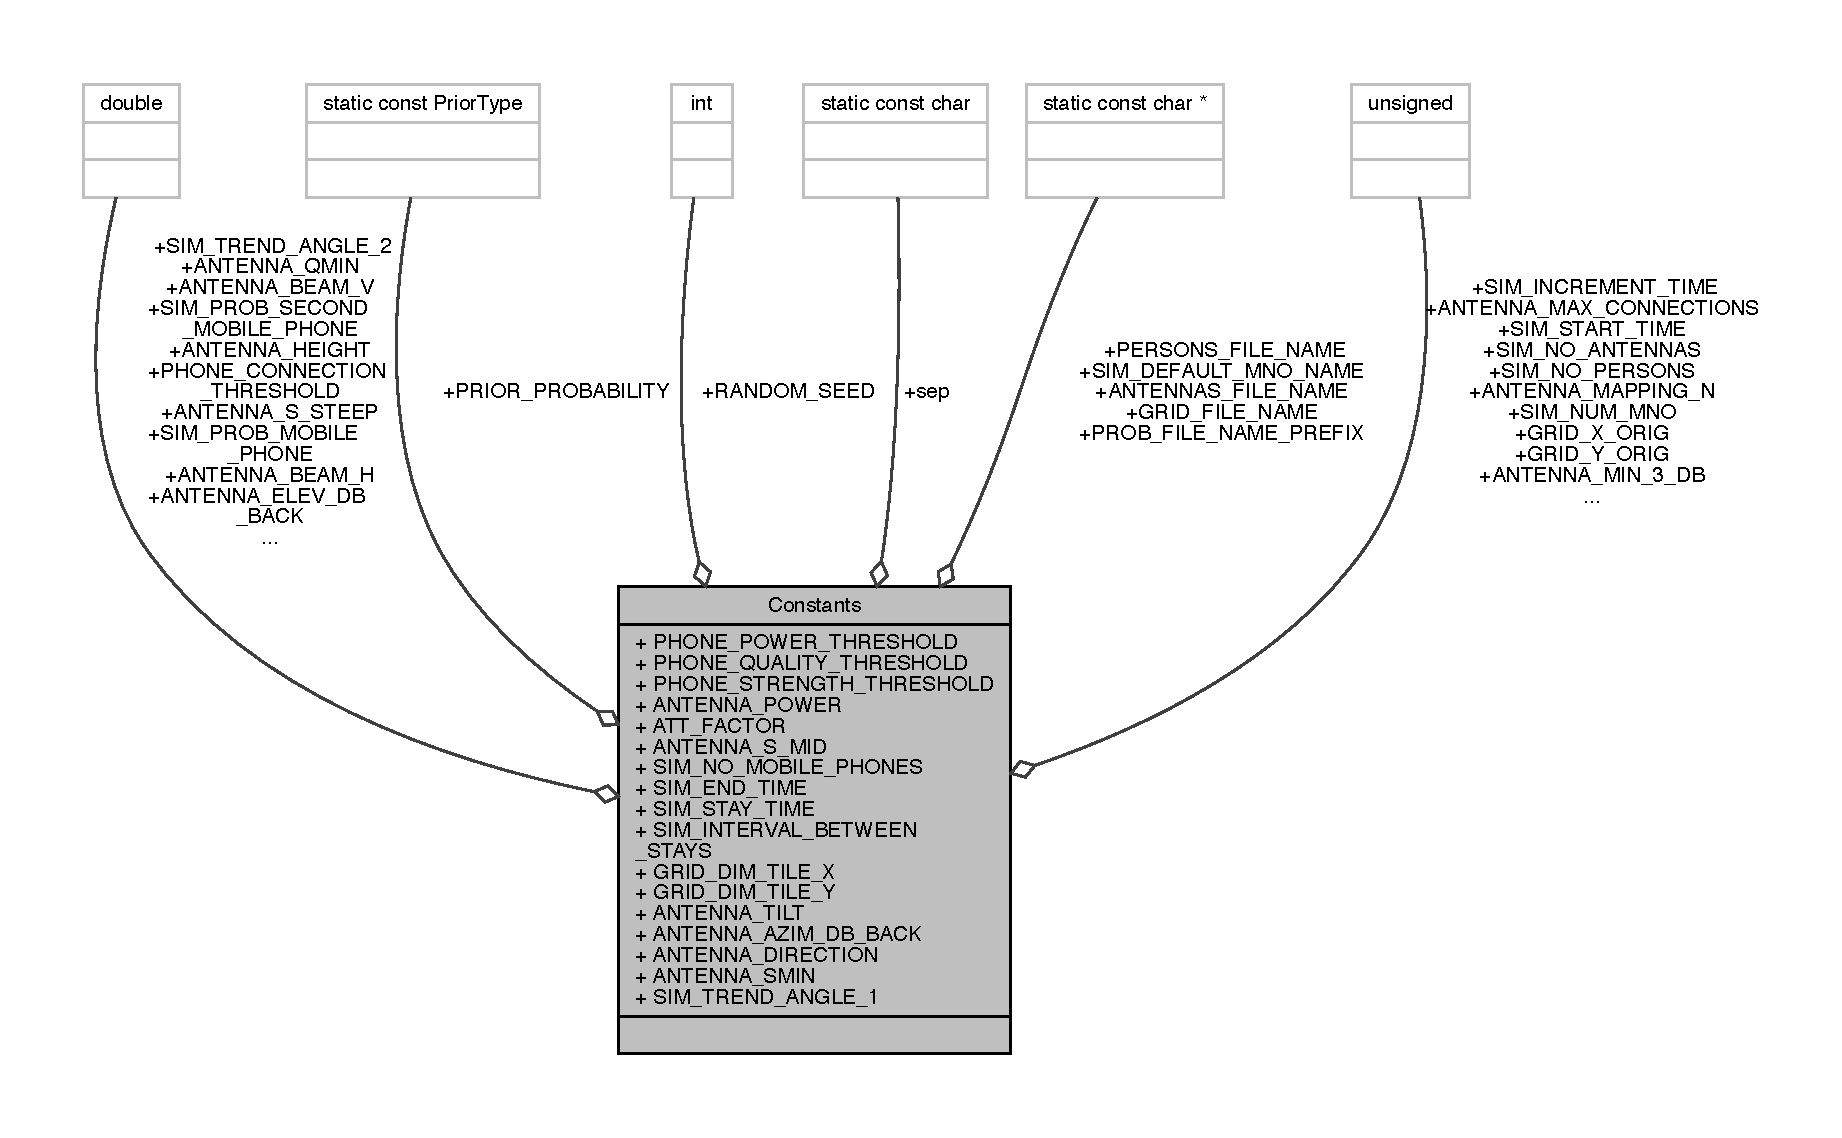
\includegraphics[width=350pt]{class_constants__coll__graph}
\end{center}
\end{figure}
\subsection*{Static Public Attributes}
\begin{DoxyCompactItemize}
\item 
static const double \hyperlink{class_constants_a1e95cbdc2db02f6147ddf8ac61a428ab}{P\+H\+O\+N\+E\+\_\+\+P\+O\+W\+E\+R\+\_\+\+T\+H\+R\+E\+S\+H\+O\+LD}
\item 
static const double \hyperlink{class_constants_a2c8a9d965bae29c19ff18c8b80260982}{P\+H\+O\+N\+E\+\_\+\+Q\+U\+A\+L\+I\+T\+Y\+\_\+\+T\+H\+R\+E\+S\+H\+O\+LD}
\item 
static const double \hyperlink{class_constants_a24b6069c3365fb95c4b853129e4d4a3e}{P\+H\+O\+N\+E\+\_\+\+S\+T\+R\+E\+N\+G\+T\+H\+\_\+\+T\+H\+R\+E\+S\+H\+O\+LD}
\item 
static const double \hyperlink{class_constants_a1cbf0a4e111b9d2e13b33e771a342b4f}{P\+H\+O\+N\+E\+\_\+\+C\+O\+N\+N\+E\+C\+T\+I\+O\+N\+\_\+\+T\+H\+R\+E\+S\+H\+O\+LD}
\item 
static const double \hyperlink{class_constants_a3f6f3825098d8eb1dc8081158c46c48a}{A\+N\+T\+E\+N\+N\+A\+\_\+\+P\+O\+W\+ER}
\item 
static const double \hyperlink{class_constants_a3738ccd4e7931b93885bdedf98528293}{A\+T\+T\+\_\+\+F\+A\+C\+T\+OR}
\item 
static const unsigned long \hyperlink{class_constants_af89a10a7d59ac020b1fa06cf673ef01f}{A\+N\+T\+E\+N\+N\+A\+\_\+\+M\+A\+X\+\_\+\+C\+O\+N\+N\+E\+C\+T\+I\+O\+NS}
\item 
static const double \hyperlink{class_constants_aea09e28749c0da58a4c831f9eabea773}{A\+N\+T\+E\+N\+N\+A\+\_\+\+S\+\_\+\+M\+ID}
\item 
static const double \hyperlink{class_constants_ae4b1b2c15d1e5bbb76464c03036c6baa}{A\+N\+T\+E\+N\+N\+A\+\_\+\+S\+\_\+\+S\+T\+E\+EP}
\item 
static const unsigned long \hyperlink{class_constants_a627fe53a717da1ca017b2467fb1dd4df}{S\+I\+M\+\_\+\+N\+O\+\_\+\+P\+E\+R\+S\+O\+NS}
\item 
static const unsigned long \hyperlink{class_constants_a0f6bc08399ad62727732e08a65c3bd0f}{S\+I\+M\+\_\+\+N\+O\+\_\+\+A\+N\+T\+E\+N\+N\+AS}
\item 
static const unsigned long \hyperlink{class_constants_a7da9e25a998c58c4388cbd45411f4232}{S\+I\+M\+\_\+\+N\+O\+\_\+\+M\+O\+B\+I\+L\+E\+\_\+\+P\+H\+O\+N\+ES}
\item 
static const unsigned long \hyperlink{class_constants_ad8a2d4817d599fd4f608e474bf1052ba}{S\+I\+M\+\_\+\+S\+T\+A\+R\+T\+\_\+\+T\+I\+ME}
\item 
static const unsigned long \hyperlink{class_constants_affb253c69b40f5979cd07383245331b7}{S\+I\+M\+\_\+\+E\+N\+D\+\_\+\+T\+I\+ME}
\item 
static const unsigned long \hyperlink{class_constants_ae689749614ecdd38b50a014400138bc2}{S\+I\+M\+\_\+\+I\+N\+C\+R\+E\+M\+E\+N\+T\+\_\+\+T\+I\+ME}
\item 
static const unsigned long \hyperlink{class_constants_a885a54aa8b2d13632ae3e8ff8e7664fb}{S\+I\+M\+\_\+\+S\+T\+A\+Y\+\_\+\+T\+I\+ME}
\item 
static const unsigned long \hyperlink{class_constants_a396cc1e9abbdf0a536886ebfd6b28045}{S\+I\+M\+\_\+\+I\+N\+T\+E\+R\+V\+A\+L\+\_\+\+B\+E\+T\+W\+E\+E\+N\+\_\+\+S\+T\+A\+YS}
\item 
static const char \hyperlink{class_constants_afc927f63cc5fbb912114d6b0f28b8b4f}{sep}
\item 
static const char $\ast$ \hyperlink{class_constants_aa2fd1c5551c8dab10dc1bd4c0cd0db8f}{G\+R\+I\+D\+\_\+\+F\+I\+L\+E\+\_\+\+N\+A\+ME}
\item 
static const unsigned long \hyperlink{class_constants_ac09062322e1ab9b6e1ca3a568b11c376}{G\+R\+I\+D\+\_\+\+X\+\_\+\+O\+R\+IG}
\item 
static const unsigned long \hyperlink{class_constants_ace48b30468931aaf452ab7a6daf573e0}{G\+R\+I\+D\+\_\+\+Y\+\_\+\+O\+R\+IG}
\item 
static const double \hyperlink{class_constants_a4400d3f97fa2e2be6091a8005efedd7f}{G\+R\+I\+D\+\_\+\+D\+I\+M\+\_\+\+T\+I\+L\+E\+\_\+X}
\item 
static const double \hyperlink{class_constants_a08f9273d844b68a74fd979d5a46d4918}{G\+R\+I\+D\+\_\+\+D\+I\+M\+\_\+\+T\+I\+L\+E\+\_\+Y}
\item 
static const char $\ast$ \hyperlink{class_constants_a3b2d3fc0ccc4636a51190bf5b297d72d}{P\+R\+O\+B\+\_\+\+F\+I\+L\+E\+\_\+\+N\+A\+M\+E\+\_\+\+P\+R\+E\+F\+IX}
\item 
static const char $\ast$ \hyperlink{class_constants_a2388516c40960223c0aef1610fd72312}{P\+E\+R\+S\+O\+N\+S\+\_\+\+F\+I\+L\+E\+\_\+\+N\+A\+ME}
\item 
static const char $\ast$ \hyperlink{class_constants_a23f758b23b88c7cfe23b278647671acb}{A\+N\+T\+E\+N\+N\+A\+S\+\_\+\+F\+I\+L\+E\+\_\+\+N\+A\+ME}
\item 
static const char $\ast$ \hyperlink{class_constants_a91fc37386abce571a0c7cd3f1b4b47c3}{O\+U\+T\+P\+U\+T\+\_\+\+D\+IR}
\item 
static const \hyperlink{_prior_type_8h_a61286c562e68de246982fc393a7c23a5}{Prior\+Type} \hyperlink{class_constants_a7b31976adc7ad0f3dbed86b205e1773d}{P\+R\+I\+O\+R\+\_\+\+P\+R\+O\+B\+A\+B\+I\+L\+I\+TY}
\item 
static const double \hyperlink{class_constants_adfe27efa61ae50b73c74b3f19c292625}{A\+N\+T\+E\+N\+N\+A\+\_\+\+H\+E\+I\+G\+HT}
\item 
static const double \hyperlink{class_constants_ad92a5c99071f0d843ee555e74c5f909a}{A\+N\+T\+E\+N\+N\+A\+\_\+\+T\+I\+LT}
\item 
static const double \hyperlink{class_constants_aa2030f2c0ec89fb7cc06b31bbb50793d}{A\+N\+T\+E\+N\+N\+A\+\_\+\+A\+Z\+I\+M\+\_\+\+D\+B\+\_\+\+B\+A\+CK}
\item 
static const double \hyperlink{class_constants_a8efdd6e1f2a25c24cb6dbff363e2d61a}{A\+N\+T\+E\+N\+N\+A\+\_\+\+E\+L\+E\+V\+\_\+\+D\+B\+\_\+\+B\+A\+CK}
\item 
static const double \hyperlink{class_constants_a4e4a0a48ad06c458ae4f3e6d0e4e6608}{A\+N\+T\+E\+N\+N\+A\+\_\+\+B\+E\+A\+M\+\_\+H}
\item 
static const double \hyperlink{class_constants_a2389355f6184d3b7903e154b46d069f5}{A\+N\+T\+E\+N\+N\+A\+\_\+\+B\+E\+A\+M\+\_\+V}
\item 
static const double \hyperlink{class_constants_ad82a10e13ae9e1cbce1cef616e47df31}{A\+N\+T\+E\+N\+N\+A\+\_\+\+D\+I\+R\+E\+C\+T\+I\+ON}
\item 
static const unsigned int \hyperlink{class_constants_a5db3a5bad9c514c994e71063dee2a798}{A\+N\+T\+E\+N\+N\+A\+\_\+\+M\+A\+P\+P\+I\+N\+G\+\_\+N}
\item 
static const unsigned int \hyperlink{class_constants_a2bda61c04e204f4a1279338fb790e1f4}{A\+N\+T\+E\+N\+N\+A\+\_\+\+M\+I\+N\+\_\+3\+\_\+\+DB}
\item 
static const double \hyperlink{class_constants_af58b693e1ab4cdb1e83399eb0f2af647}{A\+N\+T\+E\+N\+N\+A\+\_\+\+S\+M\+IN}
\item 
static const double \hyperlink{class_constants_a9149aaac071422191e4417885fd42b07}{A\+N\+T\+E\+N\+N\+A\+\_\+\+Q\+M\+IN}
\item 
static const unsigned int \hyperlink{class_constants_a763bdd9401295d6b691c93cf580e562a}{S\+I\+M\+\_\+\+N\+U\+M\+\_\+\+M\+NO}
\item 
static const char $\ast$ \hyperlink{class_constants_a186cf83e20074a889823a7f36e50ad8c}{S\+I\+M\+\_\+\+D\+E\+F\+A\+U\+L\+T\+\_\+\+M\+N\+O\+\_\+\+N\+A\+ME}
\item 
static const double \hyperlink{class_constants_a8af75c6e731c2f425cce792b33786db7}{S\+I\+M\+\_\+\+P\+R\+O\+B\+\_\+\+M\+O\+B\+I\+L\+E\+\_\+\+P\+H\+O\+NE}
\item 
static const double \hyperlink{class_constants_aafd39df52173dca1074d8c92aa5f9649}{S\+I\+M\+\_\+\+P\+R\+O\+B\+\_\+\+S\+E\+C\+O\+N\+D\+\_\+\+M\+O\+B\+I\+L\+E\+\_\+\+P\+H\+O\+NE}
\item 
static const double \hyperlink{class_constants_a97968377c9a3cf2995c37aa63d3dd505}{S\+I\+M\+\_\+\+T\+R\+E\+N\+D\+\_\+\+A\+N\+G\+L\+E\+\_\+1}
\item 
static const double \hyperlink{class_constants_a1ec9cdffb9c58a2ff1cb60f64b056835}{S\+I\+M\+\_\+\+T\+R\+E\+N\+D\+\_\+\+A\+N\+G\+L\+E\+\_\+2}
\item 
static const int \hyperlink{class_constants_ac80eccfaa8e498ad3fc6ea0a2c3d38a0}{R\+A\+N\+D\+O\+M\+\_\+\+S\+E\+ED}
\end{DoxyCompactItemize}


\subsection{Detailed Description}
These are some constants used in the process of the simulation, most of them are only used for testing and rapid development of some methods, the real values of the parameters being read from the configuration files. 

\subsection{Member Data Documentation}
\mbox{\Hypertarget{class_constants_aa2030f2c0ec89fb7cc06b31bbb50793d}\label{class_constants_aa2030f2c0ec89fb7cc06b31bbb50793d}} 
\index{Constants@{Constants}!A\+N\+T\+E\+N\+N\+A\+\_\+\+A\+Z\+I\+M\+\_\+\+D\+B\+\_\+\+B\+A\+CK@{A\+N\+T\+E\+N\+N\+A\+\_\+\+A\+Z\+I\+M\+\_\+\+D\+B\+\_\+\+B\+A\+CK}}
\index{A\+N\+T\+E\+N\+N\+A\+\_\+\+A\+Z\+I\+M\+\_\+\+D\+B\+\_\+\+B\+A\+CK@{A\+N\+T\+E\+N\+N\+A\+\_\+\+A\+Z\+I\+M\+\_\+\+D\+B\+\_\+\+B\+A\+CK}!Constants@{Constants}}
\subsubsection{\texorpdfstring{A\+N\+T\+E\+N\+N\+A\+\_\+\+A\+Z\+I\+M\+\_\+\+D\+B\+\_\+\+B\+A\+CK}{ANTENNA\_AZIM\_DB\_BACK}}
{\footnotesize\ttfamily const double Constants\+::\+A\+N\+T\+E\+N\+N\+A\+\_\+\+A\+Z\+I\+M\+\_\+\+D\+B\+\_\+\+B\+A\+CK\hspace{0.3cm}{\ttfamily [static]}}

\mbox{\Hypertarget{class_constants_a4e4a0a48ad06c458ae4f3e6d0e4e6608}\label{class_constants_a4e4a0a48ad06c458ae4f3e6d0e4e6608}} 
\index{Constants@{Constants}!A\+N\+T\+E\+N\+N\+A\+\_\+\+B\+E\+A\+M\+\_\+H@{A\+N\+T\+E\+N\+N\+A\+\_\+\+B\+E\+A\+M\+\_\+H}}
\index{A\+N\+T\+E\+N\+N\+A\+\_\+\+B\+E\+A\+M\+\_\+H@{A\+N\+T\+E\+N\+N\+A\+\_\+\+B\+E\+A\+M\+\_\+H}!Constants@{Constants}}
\subsubsection{\texorpdfstring{A\+N\+T\+E\+N\+N\+A\+\_\+\+B\+E\+A\+M\+\_\+H}{ANTENNA\_BEAM\_H}}
{\footnotesize\ttfamily const double Constants\+::\+A\+N\+T\+E\+N\+N\+A\+\_\+\+B\+E\+A\+M\+\_\+H\hspace{0.3cm}{\ttfamily [static]}}

\mbox{\Hypertarget{class_constants_a2389355f6184d3b7903e154b46d069f5}\label{class_constants_a2389355f6184d3b7903e154b46d069f5}} 
\index{Constants@{Constants}!A\+N\+T\+E\+N\+N\+A\+\_\+\+B\+E\+A\+M\+\_\+V@{A\+N\+T\+E\+N\+N\+A\+\_\+\+B\+E\+A\+M\+\_\+V}}
\index{A\+N\+T\+E\+N\+N\+A\+\_\+\+B\+E\+A\+M\+\_\+V@{A\+N\+T\+E\+N\+N\+A\+\_\+\+B\+E\+A\+M\+\_\+V}!Constants@{Constants}}
\subsubsection{\texorpdfstring{A\+N\+T\+E\+N\+N\+A\+\_\+\+B\+E\+A\+M\+\_\+V}{ANTENNA\_BEAM\_V}}
{\footnotesize\ttfamily const double Constants\+::\+A\+N\+T\+E\+N\+N\+A\+\_\+\+B\+E\+A\+M\+\_\+V\hspace{0.3cm}{\ttfamily [static]}}

\mbox{\Hypertarget{class_constants_ad82a10e13ae9e1cbce1cef616e47df31}\label{class_constants_ad82a10e13ae9e1cbce1cef616e47df31}} 
\index{Constants@{Constants}!A\+N\+T\+E\+N\+N\+A\+\_\+\+D\+I\+R\+E\+C\+T\+I\+ON@{A\+N\+T\+E\+N\+N\+A\+\_\+\+D\+I\+R\+E\+C\+T\+I\+ON}}
\index{A\+N\+T\+E\+N\+N\+A\+\_\+\+D\+I\+R\+E\+C\+T\+I\+ON@{A\+N\+T\+E\+N\+N\+A\+\_\+\+D\+I\+R\+E\+C\+T\+I\+ON}!Constants@{Constants}}
\subsubsection{\texorpdfstring{A\+N\+T\+E\+N\+N\+A\+\_\+\+D\+I\+R\+E\+C\+T\+I\+ON}{ANTENNA\_DIRECTION}}
{\footnotesize\ttfamily const double Constants\+::\+A\+N\+T\+E\+N\+N\+A\+\_\+\+D\+I\+R\+E\+C\+T\+I\+ON\hspace{0.3cm}{\ttfamily [static]}}

\mbox{\Hypertarget{class_constants_a8efdd6e1f2a25c24cb6dbff363e2d61a}\label{class_constants_a8efdd6e1f2a25c24cb6dbff363e2d61a}} 
\index{Constants@{Constants}!A\+N\+T\+E\+N\+N\+A\+\_\+\+E\+L\+E\+V\+\_\+\+D\+B\+\_\+\+B\+A\+CK@{A\+N\+T\+E\+N\+N\+A\+\_\+\+E\+L\+E\+V\+\_\+\+D\+B\+\_\+\+B\+A\+CK}}
\index{A\+N\+T\+E\+N\+N\+A\+\_\+\+E\+L\+E\+V\+\_\+\+D\+B\+\_\+\+B\+A\+CK@{A\+N\+T\+E\+N\+N\+A\+\_\+\+E\+L\+E\+V\+\_\+\+D\+B\+\_\+\+B\+A\+CK}!Constants@{Constants}}
\subsubsection{\texorpdfstring{A\+N\+T\+E\+N\+N\+A\+\_\+\+E\+L\+E\+V\+\_\+\+D\+B\+\_\+\+B\+A\+CK}{ANTENNA\_ELEV\_DB\_BACK}}
{\footnotesize\ttfamily const double Constants\+::\+A\+N\+T\+E\+N\+N\+A\+\_\+\+E\+L\+E\+V\+\_\+\+D\+B\+\_\+\+B\+A\+CK\hspace{0.3cm}{\ttfamily [static]}}

\mbox{\Hypertarget{class_constants_adfe27efa61ae50b73c74b3f19c292625}\label{class_constants_adfe27efa61ae50b73c74b3f19c292625}} 
\index{Constants@{Constants}!A\+N\+T\+E\+N\+N\+A\+\_\+\+H\+E\+I\+G\+HT@{A\+N\+T\+E\+N\+N\+A\+\_\+\+H\+E\+I\+G\+HT}}
\index{A\+N\+T\+E\+N\+N\+A\+\_\+\+H\+E\+I\+G\+HT@{A\+N\+T\+E\+N\+N\+A\+\_\+\+H\+E\+I\+G\+HT}!Constants@{Constants}}
\subsubsection{\texorpdfstring{A\+N\+T\+E\+N\+N\+A\+\_\+\+H\+E\+I\+G\+HT}{ANTENNA\_HEIGHT}}
{\footnotesize\ttfamily const double Constants\+::\+A\+N\+T\+E\+N\+N\+A\+\_\+\+H\+E\+I\+G\+HT\hspace{0.3cm}{\ttfamily [static]}}

the antenna height \mbox{\Hypertarget{class_constants_a5db3a5bad9c514c994e71063dee2a798}\label{class_constants_a5db3a5bad9c514c994e71063dee2a798}} 
\index{Constants@{Constants}!A\+N\+T\+E\+N\+N\+A\+\_\+\+M\+A\+P\+P\+I\+N\+G\+\_\+N@{A\+N\+T\+E\+N\+N\+A\+\_\+\+M\+A\+P\+P\+I\+N\+G\+\_\+N}}
\index{A\+N\+T\+E\+N\+N\+A\+\_\+\+M\+A\+P\+P\+I\+N\+G\+\_\+N@{A\+N\+T\+E\+N\+N\+A\+\_\+\+M\+A\+P\+P\+I\+N\+G\+\_\+N}!Constants@{Constants}}
\subsubsection{\texorpdfstring{A\+N\+T\+E\+N\+N\+A\+\_\+\+M\+A\+P\+P\+I\+N\+G\+\_\+N}{ANTENNA\_MAPPING\_N}}
{\footnotesize\ttfamily const unsigned int Constants\+::\+A\+N\+T\+E\+N\+N\+A\+\_\+\+M\+A\+P\+P\+I\+N\+G\+\_\+N\hspace{0.3cm}{\ttfamily [static]}}

\mbox{\Hypertarget{class_constants_af89a10a7d59ac020b1fa06cf673ef01f}\label{class_constants_af89a10a7d59ac020b1fa06cf673ef01f}} 
\index{Constants@{Constants}!A\+N\+T\+E\+N\+N\+A\+\_\+\+M\+A\+X\+\_\+\+C\+O\+N\+N\+E\+C\+T\+I\+O\+NS@{A\+N\+T\+E\+N\+N\+A\+\_\+\+M\+A\+X\+\_\+\+C\+O\+N\+N\+E\+C\+T\+I\+O\+NS}}
\index{A\+N\+T\+E\+N\+N\+A\+\_\+\+M\+A\+X\+\_\+\+C\+O\+N\+N\+E\+C\+T\+I\+O\+NS@{A\+N\+T\+E\+N\+N\+A\+\_\+\+M\+A\+X\+\_\+\+C\+O\+N\+N\+E\+C\+T\+I\+O\+NS}!Constants@{Constants}}
\subsubsection{\texorpdfstring{A\+N\+T\+E\+N\+N\+A\+\_\+\+M\+A\+X\+\_\+\+C\+O\+N\+N\+E\+C\+T\+I\+O\+NS}{ANTENNA\_MAX\_CONNECTIONS}}
{\footnotesize\ttfamily const unsigned long Constants\+::\+A\+N\+T\+E\+N\+N\+A\+\_\+\+M\+A\+X\+\_\+\+C\+O\+N\+N\+E\+C\+T\+I\+O\+NS\hspace{0.3cm}{\ttfamily [static]}}

The maximum number of devices an antenna can connect. \mbox{\Hypertarget{class_constants_a2bda61c04e204f4a1279338fb790e1f4}\label{class_constants_a2bda61c04e204f4a1279338fb790e1f4}} 
\index{Constants@{Constants}!A\+N\+T\+E\+N\+N\+A\+\_\+\+M\+I\+N\+\_\+3\+\_\+\+DB@{A\+N\+T\+E\+N\+N\+A\+\_\+\+M\+I\+N\+\_\+3\+\_\+\+DB}}
\index{A\+N\+T\+E\+N\+N\+A\+\_\+\+M\+I\+N\+\_\+3\+\_\+\+DB@{A\+N\+T\+E\+N\+N\+A\+\_\+\+M\+I\+N\+\_\+3\+\_\+\+DB}!Constants@{Constants}}
\subsubsection{\texorpdfstring{A\+N\+T\+E\+N\+N\+A\+\_\+\+M\+I\+N\+\_\+3\+\_\+\+DB}{ANTENNA\_MIN\_3\_DB}}
{\footnotesize\ttfamily const unsigned int Constants\+::\+A\+N\+T\+E\+N\+N\+A\+\_\+\+M\+I\+N\+\_\+3\+\_\+\+DB\hspace{0.3cm}{\ttfamily [static]}}

\mbox{\Hypertarget{class_constants_a3f6f3825098d8eb1dc8081158c46c48a}\label{class_constants_a3f6f3825098d8eb1dc8081158c46c48a}} 
\index{Constants@{Constants}!A\+N\+T\+E\+N\+N\+A\+\_\+\+P\+O\+W\+ER@{A\+N\+T\+E\+N\+N\+A\+\_\+\+P\+O\+W\+ER}}
\index{A\+N\+T\+E\+N\+N\+A\+\_\+\+P\+O\+W\+ER@{A\+N\+T\+E\+N\+N\+A\+\_\+\+P\+O\+W\+ER}!Constants@{Constants}}
\subsubsection{\texorpdfstring{A\+N\+T\+E\+N\+N\+A\+\_\+\+P\+O\+W\+ER}{ANTENNA\_POWER}}
{\footnotesize\ttfamily const double Constants\+::\+A\+N\+T\+E\+N\+N\+A\+\_\+\+P\+O\+W\+ER\hspace{0.3cm}{\ttfamily [static]}}

\hyperlink{class_antenna}{Antenna} power in Watts. \mbox{\Hypertarget{class_constants_a9149aaac071422191e4417885fd42b07}\label{class_constants_a9149aaac071422191e4417885fd42b07}} 
\index{Constants@{Constants}!A\+N\+T\+E\+N\+N\+A\+\_\+\+Q\+M\+IN@{A\+N\+T\+E\+N\+N\+A\+\_\+\+Q\+M\+IN}}
\index{A\+N\+T\+E\+N\+N\+A\+\_\+\+Q\+M\+IN@{A\+N\+T\+E\+N\+N\+A\+\_\+\+Q\+M\+IN}!Constants@{Constants}}
\subsubsection{\texorpdfstring{A\+N\+T\+E\+N\+N\+A\+\_\+\+Q\+M\+IN}{ANTENNA\_QMIN}}
{\footnotesize\ttfamily const double Constants\+::\+A\+N\+T\+E\+N\+N\+A\+\_\+\+Q\+M\+IN\hspace{0.3cm}{\ttfamily [static]}}

\mbox{\Hypertarget{class_constants_aea09e28749c0da58a4c831f9eabea773}\label{class_constants_aea09e28749c0da58a4c831f9eabea773}} 
\index{Constants@{Constants}!A\+N\+T\+E\+N\+N\+A\+\_\+\+S\+\_\+\+M\+ID@{A\+N\+T\+E\+N\+N\+A\+\_\+\+S\+\_\+\+M\+ID}}
\index{A\+N\+T\+E\+N\+N\+A\+\_\+\+S\+\_\+\+M\+ID@{A\+N\+T\+E\+N\+N\+A\+\_\+\+S\+\_\+\+M\+ID}!Constants@{Constants}}
\subsubsection{\texorpdfstring{A\+N\+T\+E\+N\+N\+A\+\_\+\+S\+\_\+\+M\+ID}{ANTENNA\_S\_MID}}
{\footnotesize\ttfamily const double Constants\+::\+A\+N\+T\+E\+N\+N\+A\+\_\+\+S\+\_\+\+M\+ID\hspace{0.3cm}{\ttfamily [static]}}

The Smid parameter of an antenna \mbox{\Hypertarget{class_constants_ae4b1b2c15d1e5bbb76464c03036c6baa}\label{class_constants_ae4b1b2c15d1e5bbb76464c03036c6baa}} 
\index{Constants@{Constants}!A\+N\+T\+E\+N\+N\+A\+\_\+\+S\+\_\+\+S\+T\+E\+EP@{A\+N\+T\+E\+N\+N\+A\+\_\+\+S\+\_\+\+S\+T\+E\+EP}}
\index{A\+N\+T\+E\+N\+N\+A\+\_\+\+S\+\_\+\+S\+T\+E\+EP@{A\+N\+T\+E\+N\+N\+A\+\_\+\+S\+\_\+\+S\+T\+E\+EP}!Constants@{Constants}}
\subsubsection{\texorpdfstring{A\+N\+T\+E\+N\+N\+A\+\_\+\+S\+\_\+\+S\+T\+E\+EP}{ANTENNA\_S\_STEEP}}
{\footnotesize\ttfamily const double Constants\+::\+A\+N\+T\+E\+N\+N\+A\+\_\+\+S\+\_\+\+S\+T\+E\+EP\hspace{0.3cm}{\ttfamily [static]}}

The Sstepp parameter of an antenna \mbox{\Hypertarget{class_constants_af58b693e1ab4cdb1e83399eb0f2af647}\label{class_constants_af58b693e1ab4cdb1e83399eb0f2af647}} 
\index{Constants@{Constants}!A\+N\+T\+E\+N\+N\+A\+\_\+\+S\+M\+IN@{A\+N\+T\+E\+N\+N\+A\+\_\+\+S\+M\+IN}}
\index{A\+N\+T\+E\+N\+N\+A\+\_\+\+S\+M\+IN@{A\+N\+T\+E\+N\+N\+A\+\_\+\+S\+M\+IN}!Constants@{Constants}}
\subsubsection{\texorpdfstring{A\+N\+T\+E\+N\+N\+A\+\_\+\+S\+M\+IN}{ANTENNA\_SMIN}}
{\footnotesize\ttfamily const double Constants\+::\+A\+N\+T\+E\+N\+N\+A\+\_\+\+S\+M\+IN\hspace{0.3cm}{\ttfamily [static]}}

\mbox{\Hypertarget{class_constants_ad92a5c99071f0d843ee555e74c5f909a}\label{class_constants_ad92a5c99071f0d843ee555e74c5f909a}} 
\index{Constants@{Constants}!A\+N\+T\+E\+N\+N\+A\+\_\+\+T\+I\+LT@{A\+N\+T\+E\+N\+N\+A\+\_\+\+T\+I\+LT}}
\index{A\+N\+T\+E\+N\+N\+A\+\_\+\+T\+I\+LT@{A\+N\+T\+E\+N\+N\+A\+\_\+\+T\+I\+LT}!Constants@{Constants}}
\subsubsection{\texorpdfstring{A\+N\+T\+E\+N\+N\+A\+\_\+\+T\+I\+LT}{ANTENNA\_TILT}}
{\footnotesize\ttfamily const double Constants\+::\+A\+N\+T\+E\+N\+N\+A\+\_\+\+T\+I\+LT\hspace{0.3cm}{\ttfamily [static]}}

\mbox{\Hypertarget{class_constants_a23f758b23b88c7cfe23b278647671acb}\label{class_constants_a23f758b23b88c7cfe23b278647671acb}} 
\index{Constants@{Constants}!A\+N\+T\+E\+N\+N\+A\+S\+\_\+\+F\+I\+L\+E\+\_\+\+N\+A\+ME@{A\+N\+T\+E\+N\+N\+A\+S\+\_\+\+F\+I\+L\+E\+\_\+\+N\+A\+ME}}
\index{A\+N\+T\+E\+N\+N\+A\+S\+\_\+\+F\+I\+L\+E\+\_\+\+N\+A\+ME@{A\+N\+T\+E\+N\+N\+A\+S\+\_\+\+F\+I\+L\+E\+\_\+\+N\+A\+ME}!Constants@{Constants}}
\subsubsection{\texorpdfstring{A\+N\+T\+E\+N\+N\+A\+S\+\_\+\+F\+I\+L\+E\+\_\+\+N\+A\+ME}{ANTENNAS\_FILE\_NAME}}
{\footnotesize\ttfamily const char$\ast$ Constants\+::\+A\+N\+T\+E\+N\+N\+A\+S\+\_\+\+F\+I\+L\+E\+\_\+\+N\+A\+ME\hspace{0.3cm}{\ttfamily [static]}}

The name of the file where the exact positions of the antennas are saved during simulation. They are needed for later analysis. \mbox{\Hypertarget{class_constants_a3738ccd4e7931b93885bdedf98528293}\label{class_constants_a3738ccd4e7931b93885bdedf98528293}} 
\index{Constants@{Constants}!A\+T\+T\+\_\+\+F\+A\+C\+T\+OR@{A\+T\+T\+\_\+\+F\+A\+C\+T\+OR}}
\index{A\+T\+T\+\_\+\+F\+A\+C\+T\+OR@{A\+T\+T\+\_\+\+F\+A\+C\+T\+OR}!Constants@{Constants}}
\subsubsection{\texorpdfstring{A\+T\+T\+\_\+\+F\+A\+C\+T\+OR}{ATT\_FACTOR}}
{\footnotesize\ttfamily const double Constants\+::\+A\+T\+T\+\_\+\+F\+A\+C\+T\+OR\hspace{0.3cm}{\ttfamily [static]}}

Attenuation factor of the signal. It usually takes values between 2 in open field and 6 inside buildings \mbox{\Hypertarget{class_constants_a4400d3f97fa2e2be6091a8005efedd7f}\label{class_constants_a4400d3f97fa2e2be6091a8005efedd7f}} 
\index{Constants@{Constants}!G\+R\+I\+D\+\_\+\+D\+I\+M\+\_\+\+T\+I\+L\+E\+\_\+X@{G\+R\+I\+D\+\_\+\+D\+I\+M\+\_\+\+T\+I\+L\+E\+\_\+X}}
\index{G\+R\+I\+D\+\_\+\+D\+I\+M\+\_\+\+T\+I\+L\+E\+\_\+X@{G\+R\+I\+D\+\_\+\+D\+I\+M\+\_\+\+T\+I\+L\+E\+\_\+X}!Constants@{Constants}}
\subsubsection{\texorpdfstring{G\+R\+I\+D\+\_\+\+D\+I\+M\+\_\+\+T\+I\+L\+E\+\_\+X}{GRID\_DIM\_TILE\_X}}
{\footnotesize\ttfamily const double Constants\+::\+G\+R\+I\+D\+\_\+\+D\+I\+M\+\_\+\+T\+I\+L\+E\+\_\+X\hspace{0.3cm}{\ttfamily [static]}}

\mbox{\Hypertarget{class_constants_a08f9273d844b68a74fd979d5a46d4918}\label{class_constants_a08f9273d844b68a74fd979d5a46d4918}} 
\index{Constants@{Constants}!G\+R\+I\+D\+\_\+\+D\+I\+M\+\_\+\+T\+I\+L\+E\+\_\+Y@{G\+R\+I\+D\+\_\+\+D\+I\+M\+\_\+\+T\+I\+L\+E\+\_\+Y}}
\index{G\+R\+I\+D\+\_\+\+D\+I\+M\+\_\+\+T\+I\+L\+E\+\_\+Y@{G\+R\+I\+D\+\_\+\+D\+I\+M\+\_\+\+T\+I\+L\+E\+\_\+Y}!Constants@{Constants}}
\subsubsection{\texorpdfstring{G\+R\+I\+D\+\_\+\+D\+I\+M\+\_\+\+T\+I\+L\+E\+\_\+Y}{GRID\_DIM\_TILE\_Y}}
{\footnotesize\ttfamily const double Constants\+::\+G\+R\+I\+D\+\_\+\+D\+I\+M\+\_\+\+T\+I\+L\+E\+\_\+Y\hspace{0.3cm}{\ttfamily [static]}}

\mbox{\Hypertarget{class_constants_aa2fd1c5551c8dab10dc1bd4c0cd0db8f}\label{class_constants_aa2fd1c5551c8dab10dc1bd4c0cd0db8f}} 
\index{Constants@{Constants}!G\+R\+I\+D\+\_\+\+F\+I\+L\+E\+\_\+\+N\+A\+ME@{G\+R\+I\+D\+\_\+\+F\+I\+L\+E\+\_\+\+N\+A\+ME}}
\index{G\+R\+I\+D\+\_\+\+F\+I\+L\+E\+\_\+\+N\+A\+ME@{G\+R\+I\+D\+\_\+\+F\+I\+L\+E\+\_\+\+N\+A\+ME}!Constants@{Constants}}
\subsubsection{\texorpdfstring{G\+R\+I\+D\+\_\+\+F\+I\+L\+E\+\_\+\+N\+A\+ME}{GRID\_FILE\_NAME}}
{\footnotesize\ttfamily const char$\ast$ Constants\+::\+G\+R\+I\+D\+\_\+\+F\+I\+L\+E\+\_\+\+N\+A\+ME\hspace{0.3cm}{\ttfamily [static]}}

The name of the file where the description of the grid is saved \mbox{\Hypertarget{class_constants_ac09062322e1ab9b6e1ca3a568b11c376}\label{class_constants_ac09062322e1ab9b6e1ca3a568b11c376}} 
\index{Constants@{Constants}!G\+R\+I\+D\+\_\+\+X\+\_\+\+O\+R\+IG@{G\+R\+I\+D\+\_\+\+X\+\_\+\+O\+R\+IG}}
\index{G\+R\+I\+D\+\_\+\+X\+\_\+\+O\+R\+IG@{G\+R\+I\+D\+\_\+\+X\+\_\+\+O\+R\+IG}!Constants@{Constants}}
\subsubsection{\texorpdfstring{G\+R\+I\+D\+\_\+\+X\+\_\+\+O\+R\+IG}{GRID\_X\_ORIG}}
{\footnotesize\ttfamily const unsigned long Constants\+::\+G\+R\+I\+D\+\_\+\+X\+\_\+\+O\+R\+IG\hspace{0.3cm}{\ttfamily [static]}}

\mbox{\Hypertarget{class_constants_ace48b30468931aaf452ab7a6daf573e0}\label{class_constants_ace48b30468931aaf452ab7a6daf573e0}} 
\index{Constants@{Constants}!G\+R\+I\+D\+\_\+\+Y\+\_\+\+O\+R\+IG@{G\+R\+I\+D\+\_\+\+Y\+\_\+\+O\+R\+IG}}
\index{G\+R\+I\+D\+\_\+\+Y\+\_\+\+O\+R\+IG@{G\+R\+I\+D\+\_\+\+Y\+\_\+\+O\+R\+IG}!Constants@{Constants}}
\subsubsection{\texorpdfstring{G\+R\+I\+D\+\_\+\+Y\+\_\+\+O\+R\+IG}{GRID\_Y\_ORIG}}
{\footnotesize\ttfamily const unsigned long Constants\+::\+G\+R\+I\+D\+\_\+\+Y\+\_\+\+O\+R\+IG\hspace{0.3cm}{\ttfamily [static]}}

\mbox{\Hypertarget{class_constants_a91fc37386abce571a0c7cd3f1b4b47c3}\label{class_constants_a91fc37386abce571a0c7cd3f1b4b47c3}} 
\index{Constants@{Constants}!O\+U\+T\+P\+U\+T\+\_\+\+D\+IR@{O\+U\+T\+P\+U\+T\+\_\+\+D\+IR}}
\index{O\+U\+T\+P\+U\+T\+\_\+\+D\+IR@{O\+U\+T\+P\+U\+T\+\_\+\+D\+IR}!Constants@{Constants}}
\subsubsection{\texorpdfstring{O\+U\+T\+P\+U\+T\+\_\+\+D\+IR}{OUTPUT\_DIR}}
{\footnotesize\ttfamily const char$\ast$ Constants\+::\+O\+U\+T\+P\+U\+T\+\_\+\+D\+IR\hspace{0.3cm}{\ttfamily [static]}}

The name of the folder where the output fle will be saved \mbox{\Hypertarget{class_constants_a2388516c40960223c0aef1610fd72312}\label{class_constants_a2388516c40960223c0aef1610fd72312}} 
\index{Constants@{Constants}!P\+E\+R\+S\+O\+N\+S\+\_\+\+F\+I\+L\+E\+\_\+\+N\+A\+ME@{P\+E\+R\+S\+O\+N\+S\+\_\+\+F\+I\+L\+E\+\_\+\+N\+A\+ME}}
\index{P\+E\+R\+S\+O\+N\+S\+\_\+\+F\+I\+L\+E\+\_\+\+N\+A\+ME@{P\+E\+R\+S\+O\+N\+S\+\_\+\+F\+I\+L\+E\+\_\+\+N\+A\+ME}!Constants@{Constants}}
\subsubsection{\texorpdfstring{P\+E\+R\+S\+O\+N\+S\+\_\+\+F\+I\+L\+E\+\_\+\+N\+A\+ME}{PERSONS\_FILE\_NAME}}
{\footnotesize\ttfamily const char$\ast$ Constants\+::\+P\+E\+R\+S\+O\+N\+S\+\_\+\+F\+I\+L\+E\+\_\+\+N\+A\+ME\hspace{0.3cm}{\ttfamily [static]}}

The name of the file where the exact positions of the persons are saved during simulation. They are needed for later analysis. \mbox{\Hypertarget{class_constants_a1cbf0a4e111b9d2e13b33e771a342b4f}\label{class_constants_a1cbf0a4e111b9d2e13b33e771a342b4f}} 
\index{Constants@{Constants}!P\+H\+O\+N\+E\+\_\+\+C\+O\+N\+N\+E\+C\+T\+I\+O\+N\+\_\+\+T\+H\+R\+E\+S\+H\+O\+LD@{P\+H\+O\+N\+E\+\_\+\+C\+O\+N\+N\+E\+C\+T\+I\+O\+N\+\_\+\+T\+H\+R\+E\+S\+H\+O\+LD}}
\index{P\+H\+O\+N\+E\+\_\+\+C\+O\+N\+N\+E\+C\+T\+I\+O\+N\+\_\+\+T\+H\+R\+E\+S\+H\+O\+LD@{P\+H\+O\+N\+E\+\_\+\+C\+O\+N\+N\+E\+C\+T\+I\+O\+N\+\_\+\+T\+H\+R\+E\+S\+H\+O\+LD}!Constants@{Constants}}
\subsubsection{\texorpdfstring{P\+H\+O\+N\+E\+\_\+\+C\+O\+N\+N\+E\+C\+T\+I\+O\+N\+\_\+\+T\+H\+R\+E\+S\+H\+O\+LD}{PHONE\_CONNECTION\_THRESHOLD}}
{\footnotesize\ttfamily const double Constants\+::\+P\+H\+O\+N\+E\+\_\+\+C\+O\+N\+N\+E\+C\+T\+I\+O\+N\+\_\+\+T\+H\+R\+E\+S\+H\+O\+LD\hspace{0.3cm}{\ttfamily [static]}}

This value is interpreted according to the connection type\+:
\begin{DoxyItemize}
\item if the connection uses power it is the minimum value of the signal power received by a phone not considered as noise. Below this value the signal is unusable and the connection between a mobile phone and an antenna is not possible.
\item if the connection uses signal quality it is the minimum value of the signal quality received by a phone not considered as noise. Below this value the signal is unusable and the connection between a mobile phone and an antenna is not possible.
\item if the connection uses signal strength it is the minimum value of the signal strength received by a phone not considered as noise. Below this value the signal is unusable and the connection between a mobile phone and an antenna is not possible. 
\end{DoxyItemize}\mbox{\Hypertarget{class_constants_a1e95cbdc2db02f6147ddf8ac61a428ab}\label{class_constants_a1e95cbdc2db02f6147ddf8ac61a428ab}} 
\index{Constants@{Constants}!P\+H\+O\+N\+E\+\_\+\+P\+O\+W\+E\+R\+\_\+\+T\+H\+R\+E\+S\+H\+O\+LD@{P\+H\+O\+N\+E\+\_\+\+P\+O\+W\+E\+R\+\_\+\+T\+H\+R\+E\+S\+H\+O\+LD}}
\index{P\+H\+O\+N\+E\+\_\+\+P\+O\+W\+E\+R\+\_\+\+T\+H\+R\+E\+S\+H\+O\+LD@{P\+H\+O\+N\+E\+\_\+\+P\+O\+W\+E\+R\+\_\+\+T\+H\+R\+E\+S\+H\+O\+LD}!Constants@{Constants}}
\subsubsection{\texorpdfstring{P\+H\+O\+N\+E\+\_\+\+P\+O\+W\+E\+R\+\_\+\+T\+H\+R\+E\+S\+H\+O\+LD}{PHONE\_POWER\_THRESHOLD}}
{\footnotesize\ttfamily const double Constants\+::\+P\+H\+O\+N\+E\+\_\+\+P\+O\+W\+E\+R\+\_\+\+T\+H\+R\+E\+S\+H\+O\+LD\hspace{0.3cm}{\ttfamily [static]}}

If the signal received by a mobile device has a power below this level, the signal is considered only noise and unusable. \mbox{\Hypertarget{class_constants_a2c8a9d965bae29c19ff18c8b80260982}\label{class_constants_a2c8a9d965bae29c19ff18c8b80260982}} 
\index{Constants@{Constants}!P\+H\+O\+N\+E\+\_\+\+Q\+U\+A\+L\+I\+T\+Y\+\_\+\+T\+H\+R\+E\+S\+H\+O\+LD@{P\+H\+O\+N\+E\+\_\+\+Q\+U\+A\+L\+I\+T\+Y\+\_\+\+T\+H\+R\+E\+S\+H\+O\+LD}}
\index{P\+H\+O\+N\+E\+\_\+\+Q\+U\+A\+L\+I\+T\+Y\+\_\+\+T\+H\+R\+E\+S\+H\+O\+LD@{P\+H\+O\+N\+E\+\_\+\+Q\+U\+A\+L\+I\+T\+Y\+\_\+\+T\+H\+R\+E\+S\+H\+O\+LD}!Constants@{Constants}}
\subsubsection{\texorpdfstring{P\+H\+O\+N\+E\+\_\+\+Q\+U\+A\+L\+I\+T\+Y\+\_\+\+T\+H\+R\+E\+S\+H\+O\+LD}{PHONE\_QUALITY\_THRESHOLD}}
{\footnotesize\ttfamily const double Constants\+::\+P\+H\+O\+N\+E\+\_\+\+Q\+U\+A\+L\+I\+T\+Y\+\_\+\+T\+H\+R\+E\+S\+H\+O\+LD\hspace{0.3cm}{\ttfamily [static]}}

If the signal received by a mobile device has a quality below this level, the signal is considered only noise and unusable. \mbox{\Hypertarget{class_constants_a24b6069c3365fb95c4b853129e4d4a3e}\label{class_constants_a24b6069c3365fb95c4b853129e4d4a3e}} 
\index{Constants@{Constants}!P\+H\+O\+N\+E\+\_\+\+S\+T\+R\+E\+N\+G\+T\+H\+\_\+\+T\+H\+R\+E\+S\+H\+O\+LD@{P\+H\+O\+N\+E\+\_\+\+S\+T\+R\+E\+N\+G\+T\+H\+\_\+\+T\+H\+R\+E\+S\+H\+O\+LD}}
\index{P\+H\+O\+N\+E\+\_\+\+S\+T\+R\+E\+N\+G\+T\+H\+\_\+\+T\+H\+R\+E\+S\+H\+O\+LD@{P\+H\+O\+N\+E\+\_\+\+S\+T\+R\+E\+N\+G\+T\+H\+\_\+\+T\+H\+R\+E\+S\+H\+O\+LD}!Constants@{Constants}}
\subsubsection{\texorpdfstring{P\+H\+O\+N\+E\+\_\+\+S\+T\+R\+E\+N\+G\+T\+H\+\_\+\+T\+H\+R\+E\+S\+H\+O\+LD}{PHONE\_STRENGTH\_THRESHOLD}}
{\footnotesize\ttfamily const double Constants\+::\+P\+H\+O\+N\+E\+\_\+\+S\+T\+R\+E\+N\+G\+T\+H\+\_\+\+T\+H\+R\+E\+S\+H\+O\+LD\hspace{0.3cm}{\ttfamily [static]}}

If the signal received by a mobile device has a quality below this level, the signal is considered only noise and unusable. \mbox{\Hypertarget{class_constants_a7b31976adc7ad0f3dbed86b205e1773d}\label{class_constants_a7b31976adc7ad0f3dbed86b205e1773d}} 
\index{Constants@{Constants}!P\+R\+I\+O\+R\+\_\+\+P\+R\+O\+B\+A\+B\+I\+L\+I\+TY@{P\+R\+I\+O\+R\+\_\+\+P\+R\+O\+B\+A\+B\+I\+L\+I\+TY}}
\index{P\+R\+I\+O\+R\+\_\+\+P\+R\+O\+B\+A\+B\+I\+L\+I\+TY@{P\+R\+I\+O\+R\+\_\+\+P\+R\+O\+B\+A\+B\+I\+L\+I\+TY}!Constants@{Constants}}
\subsubsection{\texorpdfstring{P\+R\+I\+O\+R\+\_\+\+P\+R\+O\+B\+A\+B\+I\+L\+I\+TY}{PRIOR\_PROBABILITY}}
{\footnotesize\ttfamily const \hyperlink{_prior_type_8h_a61286c562e68de246982fc393a7c23a5}{Prior\+Type} Constants\+::\+P\+R\+I\+O\+R\+\_\+\+P\+R\+O\+B\+A\+B\+I\+L\+I\+TY\hspace{0.3cm}{\ttfamily [static]}}

Indicates how the prior probability is computed\+: uniform, register, network \mbox{\Hypertarget{class_constants_a3b2d3fc0ccc4636a51190bf5b297d72d}\label{class_constants_a3b2d3fc0ccc4636a51190bf5b297d72d}} 
\index{Constants@{Constants}!P\+R\+O\+B\+\_\+\+F\+I\+L\+E\+\_\+\+N\+A\+M\+E\+\_\+\+P\+R\+E\+F\+IX@{P\+R\+O\+B\+\_\+\+F\+I\+L\+E\+\_\+\+N\+A\+M\+E\+\_\+\+P\+R\+E\+F\+IX}}
\index{P\+R\+O\+B\+\_\+\+F\+I\+L\+E\+\_\+\+N\+A\+M\+E\+\_\+\+P\+R\+E\+F\+IX@{P\+R\+O\+B\+\_\+\+F\+I\+L\+E\+\_\+\+N\+A\+M\+E\+\_\+\+P\+R\+E\+F\+IX}!Constants@{Constants}}
\subsubsection{\texorpdfstring{P\+R\+O\+B\+\_\+\+F\+I\+L\+E\+\_\+\+N\+A\+M\+E\+\_\+\+P\+R\+E\+F\+IX}{PROB\_FILE\_NAME\_PREFIX}}
{\footnotesize\ttfamily const char$\ast$ Constants\+::\+P\+R\+O\+B\+\_\+\+F\+I\+L\+E\+\_\+\+N\+A\+M\+E\+\_\+\+P\+R\+E\+F\+IX\hspace{0.3cm}{\ttfamily [static]}}

The name of the file where the probabilities of mobile phones locations are saved \mbox{\Hypertarget{class_constants_ac80eccfaa8e498ad3fc6ea0a2c3d38a0}\label{class_constants_ac80eccfaa8e498ad3fc6ea0a2c3d38a0}} 
\index{Constants@{Constants}!R\+A\+N\+D\+O\+M\+\_\+\+S\+E\+ED@{R\+A\+N\+D\+O\+M\+\_\+\+S\+E\+ED}}
\index{R\+A\+N\+D\+O\+M\+\_\+\+S\+E\+ED@{R\+A\+N\+D\+O\+M\+\_\+\+S\+E\+ED}!Constants@{Constants}}
\subsubsection{\texorpdfstring{R\+A\+N\+D\+O\+M\+\_\+\+S\+E\+ED}{RANDOM\_SEED}}
{\footnotesize\ttfamily const int Constants\+::\+R\+A\+N\+D\+O\+M\+\_\+\+S\+E\+ED\hspace{0.3cm}{\ttfamily [static]}}

\mbox{\Hypertarget{class_constants_afc927f63cc5fbb912114d6b0f28b8b4f}\label{class_constants_afc927f63cc5fbb912114d6b0f28b8b4f}} 
\index{Constants@{Constants}!sep@{sep}}
\index{sep@{sep}!Constants@{Constants}}
\subsubsection{\texorpdfstring{sep}{sep}}
{\footnotesize\ttfamily const char Constants\+::sep\hspace{0.3cm}{\ttfamily [static]}}

The separator used when information is saved in output files \mbox{\Hypertarget{class_constants_a186cf83e20074a889823a7f36e50ad8c}\label{class_constants_a186cf83e20074a889823a7f36e50ad8c}} 
\index{Constants@{Constants}!S\+I\+M\+\_\+\+D\+E\+F\+A\+U\+L\+T\+\_\+\+M\+N\+O\+\_\+\+N\+A\+ME@{S\+I\+M\+\_\+\+D\+E\+F\+A\+U\+L\+T\+\_\+\+M\+N\+O\+\_\+\+N\+A\+ME}}
\index{S\+I\+M\+\_\+\+D\+E\+F\+A\+U\+L\+T\+\_\+\+M\+N\+O\+\_\+\+N\+A\+ME@{S\+I\+M\+\_\+\+D\+E\+F\+A\+U\+L\+T\+\_\+\+M\+N\+O\+\_\+\+N\+A\+ME}!Constants@{Constants}}
\subsubsection{\texorpdfstring{S\+I\+M\+\_\+\+D\+E\+F\+A\+U\+L\+T\+\_\+\+M\+N\+O\+\_\+\+N\+A\+ME}{SIM\_DEFAULT\_MNO\_NAME}}
{\footnotesize\ttfamily const char$\ast$ Constants\+::\+S\+I\+M\+\_\+\+D\+E\+F\+A\+U\+L\+T\+\_\+\+M\+N\+O\+\_\+\+N\+A\+ME\hspace{0.3cm}{\ttfamily [static]}}

\mbox{\Hypertarget{class_constants_affb253c69b40f5979cd07383245331b7}\label{class_constants_affb253c69b40f5979cd07383245331b7}} 
\index{Constants@{Constants}!S\+I\+M\+\_\+\+E\+N\+D\+\_\+\+T\+I\+ME@{S\+I\+M\+\_\+\+E\+N\+D\+\_\+\+T\+I\+ME}}
\index{S\+I\+M\+\_\+\+E\+N\+D\+\_\+\+T\+I\+ME@{S\+I\+M\+\_\+\+E\+N\+D\+\_\+\+T\+I\+ME}!Constants@{Constants}}
\subsubsection{\texorpdfstring{S\+I\+M\+\_\+\+E\+N\+D\+\_\+\+T\+I\+ME}{SIM\_END\_TIME}}
{\footnotesize\ttfamily const unsigned long Constants\+::\+S\+I\+M\+\_\+\+E\+N\+D\+\_\+\+T\+I\+ME\hspace{0.3cm}{\ttfamily [static]}}

Default ending time of a simulation \mbox{\Hypertarget{class_constants_ae689749614ecdd38b50a014400138bc2}\label{class_constants_ae689749614ecdd38b50a014400138bc2}} 
\index{Constants@{Constants}!S\+I\+M\+\_\+\+I\+N\+C\+R\+E\+M\+E\+N\+T\+\_\+\+T\+I\+ME@{S\+I\+M\+\_\+\+I\+N\+C\+R\+E\+M\+E\+N\+T\+\_\+\+T\+I\+ME}}
\index{S\+I\+M\+\_\+\+I\+N\+C\+R\+E\+M\+E\+N\+T\+\_\+\+T\+I\+ME@{S\+I\+M\+\_\+\+I\+N\+C\+R\+E\+M\+E\+N\+T\+\_\+\+T\+I\+ME}!Constants@{Constants}}
\subsubsection{\texorpdfstring{S\+I\+M\+\_\+\+I\+N\+C\+R\+E\+M\+E\+N\+T\+\_\+\+T\+I\+ME}{SIM\_INCREMENT\_TIME}}
{\footnotesize\ttfamily const unsigned long Constants\+::\+S\+I\+M\+\_\+\+I\+N\+C\+R\+E\+M\+E\+N\+T\+\_\+\+T\+I\+ME\hspace{0.3cm}{\ttfamily [static]}}

Default time increment for a simulation \mbox{\Hypertarget{class_constants_a396cc1e9abbdf0a536886ebfd6b28045}\label{class_constants_a396cc1e9abbdf0a536886ebfd6b28045}} 
\index{Constants@{Constants}!S\+I\+M\+\_\+\+I\+N\+T\+E\+R\+V\+A\+L\+\_\+\+B\+E\+T\+W\+E\+E\+N\+\_\+\+S\+T\+A\+YS@{S\+I\+M\+\_\+\+I\+N\+T\+E\+R\+V\+A\+L\+\_\+\+B\+E\+T\+W\+E\+E\+N\+\_\+\+S\+T\+A\+YS}}
\index{S\+I\+M\+\_\+\+I\+N\+T\+E\+R\+V\+A\+L\+\_\+\+B\+E\+T\+W\+E\+E\+N\+\_\+\+S\+T\+A\+YS@{S\+I\+M\+\_\+\+I\+N\+T\+E\+R\+V\+A\+L\+\_\+\+B\+E\+T\+W\+E\+E\+N\+\_\+\+S\+T\+A\+YS}!Constants@{Constants}}
\subsubsection{\texorpdfstring{S\+I\+M\+\_\+\+I\+N\+T\+E\+R\+V\+A\+L\+\_\+\+B\+E\+T\+W\+E\+E\+N\+\_\+\+S\+T\+A\+YS}{SIM\_INTERVAL\_BETWEEN\_STAYS}}
{\footnotesize\ttfamily const unsigned long Constants\+::\+S\+I\+M\+\_\+\+I\+N\+T\+E\+R\+V\+A\+L\+\_\+\+B\+E\+T\+W\+E\+E\+N\+\_\+\+S\+T\+A\+YS\hspace{0.3cm}{\ttfamily [static]}}

\mbox{\Hypertarget{class_constants_a0f6bc08399ad62727732e08a65c3bd0f}\label{class_constants_a0f6bc08399ad62727732e08a65c3bd0f}} 
\index{Constants@{Constants}!S\+I\+M\+\_\+\+N\+O\+\_\+\+A\+N\+T\+E\+N\+N\+AS@{S\+I\+M\+\_\+\+N\+O\+\_\+\+A\+N\+T\+E\+N\+N\+AS}}
\index{S\+I\+M\+\_\+\+N\+O\+\_\+\+A\+N\+T\+E\+N\+N\+AS@{S\+I\+M\+\_\+\+N\+O\+\_\+\+A\+N\+T\+E\+N\+N\+AS}!Constants@{Constants}}
\subsubsection{\texorpdfstring{S\+I\+M\+\_\+\+N\+O\+\_\+\+A\+N\+T\+E\+N\+N\+AS}{SIM\_NO\_ANTENNAS}}
{\footnotesize\ttfamily const unsigned long Constants\+::\+S\+I\+M\+\_\+\+N\+O\+\_\+\+A\+N\+T\+E\+N\+N\+AS\hspace{0.3cm}{\ttfamily [static]}}

The number of antenna used for a simulation \mbox{\Hypertarget{class_constants_a7da9e25a998c58c4388cbd45411f4232}\label{class_constants_a7da9e25a998c58c4388cbd45411f4232}} 
\index{Constants@{Constants}!S\+I\+M\+\_\+\+N\+O\+\_\+\+M\+O\+B\+I\+L\+E\+\_\+\+P\+H\+O\+N\+ES@{S\+I\+M\+\_\+\+N\+O\+\_\+\+M\+O\+B\+I\+L\+E\+\_\+\+P\+H\+O\+N\+ES}}
\index{S\+I\+M\+\_\+\+N\+O\+\_\+\+M\+O\+B\+I\+L\+E\+\_\+\+P\+H\+O\+N\+ES@{S\+I\+M\+\_\+\+N\+O\+\_\+\+M\+O\+B\+I\+L\+E\+\_\+\+P\+H\+O\+N\+ES}!Constants@{Constants}}
\subsubsection{\texorpdfstring{S\+I\+M\+\_\+\+N\+O\+\_\+\+M\+O\+B\+I\+L\+E\+\_\+\+P\+H\+O\+N\+ES}{SIM\_NO\_MOBILE\_PHONES}}
{\footnotesize\ttfamily const unsigned long Constants\+::\+S\+I\+M\+\_\+\+N\+O\+\_\+\+M\+O\+B\+I\+L\+E\+\_\+\+P\+H\+O\+N\+ES\hspace{0.3cm}{\ttfamily [static]}}

The number of the mobile devices used for a simulation \mbox{\Hypertarget{class_constants_a627fe53a717da1ca017b2467fb1dd4df}\label{class_constants_a627fe53a717da1ca017b2467fb1dd4df}} 
\index{Constants@{Constants}!S\+I\+M\+\_\+\+N\+O\+\_\+\+P\+E\+R\+S\+O\+NS@{S\+I\+M\+\_\+\+N\+O\+\_\+\+P\+E\+R\+S\+O\+NS}}
\index{S\+I\+M\+\_\+\+N\+O\+\_\+\+P\+E\+R\+S\+O\+NS@{S\+I\+M\+\_\+\+N\+O\+\_\+\+P\+E\+R\+S\+O\+NS}!Constants@{Constants}}
\subsubsection{\texorpdfstring{S\+I\+M\+\_\+\+N\+O\+\_\+\+P\+E\+R\+S\+O\+NS}{SIM\_NO\_PERSONS}}
{\footnotesize\ttfamily const unsigned long Constants\+::\+S\+I\+M\+\_\+\+N\+O\+\_\+\+P\+E\+R\+S\+O\+NS\hspace{0.3cm}{\ttfamily [static]}}

The number of persons used for a simulation \mbox{\Hypertarget{class_constants_a763bdd9401295d6b691c93cf580e562a}\label{class_constants_a763bdd9401295d6b691c93cf580e562a}} 
\index{Constants@{Constants}!S\+I\+M\+\_\+\+N\+U\+M\+\_\+\+M\+NO@{S\+I\+M\+\_\+\+N\+U\+M\+\_\+\+M\+NO}}
\index{S\+I\+M\+\_\+\+N\+U\+M\+\_\+\+M\+NO@{S\+I\+M\+\_\+\+N\+U\+M\+\_\+\+M\+NO}!Constants@{Constants}}
\subsubsection{\texorpdfstring{S\+I\+M\+\_\+\+N\+U\+M\+\_\+\+M\+NO}{SIM\_NUM\_MNO}}
{\footnotesize\ttfamily const unsigned int Constants\+::\+S\+I\+M\+\_\+\+N\+U\+M\+\_\+\+M\+NO\hspace{0.3cm}{\ttfamily [static]}}

\mbox{\Hypertarget{class_constants_a8af75c6e731c2f425cce792b33786db7}\label{class_constants_a8af75c6e731c2f425cce792b33786db7}} 
\index{Constants@{Constants}!S\+I\+M\+\_\+\+P\+R\+O\+B\+\_\+\+M\+O\+B\+I\+L\+E\+\_\+\+P\+H\+O\+NE@{S\+I\+M\+\_\+\+P\+R\+O\+B\+\_\+\+M\+O\+B\+I\+L\+E\+\_\+\+P\+H\+O\+NE}}
\index{S\+I\+M\+\_\+\+P\+R\+O\+B\+\_\+\+M\+O\+B\+I\+L\+E\+\_\+\+P\+H\+O\+NE@{S\+I\+M\+\_\+\+P\+R\+O\+B\+\_\+\+M\+O\+B\+I\+L\+E\+\_\+\+P\+H\+O\+NE}!Constants@{Constants}}
\subsubsection{\texorpdfstring{S\+I\+M\+\_\+\+P\+R\+O\+B\+\_\+\+M\+O\+B\+I\+L\+E\+\_\+\+P\+H\+O\+NE}{SIM\_PROB\_MOBILE\_PHONE}}
{\footnotesize\ttfamily const double Constants\+::\+S\+I\+M\+\_\+\+P\+R\+O\+B\+\_\+\+M\+O\+B\+I\+L\+E\+\_\+\+P\+H\+O\+NE\hspace{0.3cm}{\ttfamily [static]}}

\mbox{\Hypertarget{class_constants_aafd39df52173dca1074d8c92aa5f9649}\label{class_constants_aafd39df52173dca1074d8c92aa5f9649}} 
\index{Constants@{Constants}!S\+I\+M\+\_\+\+P\+R\+O\+B\+\_\+\+S\+E\+C\+O\+N\+D\+\_\+\+M\+O\+B\+I\+L\+E\+\_\+\+P\+H\+O\+NE@{S\+I\+M\+\_\+\+P\+R\+O\+B\+\_\+\+S\+E\+C\+O\+N\+D\+\_\+\+M\+O\+B\+I\+L\+E\+\_\+\+P\+H\+O\+NE}}
\index{S\+I\+M\+\_\+\+P\+R\+O\+B\+\_\+\+S\+E\+C\+O\+N\+D\+\_\+\+M\+O\+B\+I\+L\+E\+\_\+\+P\+H\+O\+NE@{S\+I\+M\+\_\+\+P\+R\+O\+B\+\_\+\+S\+E\+C\+O\+N\+D\+\_\+\+M\+O\+B\+I\+L\+E\+\_\+\+P\+H\+O\+NE}!Constants@{Constants}}
\subsubsection{\texorpdfstring{S\+I\+M\+\_\+\+P\+R\+O\+B\+\_\+\+S\+E\+C\+O\+N\+D\+\_\+\+M\+O\+B\+I\+L\+E\+\_\+\+P\+H\+O\+NE}{SIM\_PROB\_SECOND\_MOBILE\_PHONE}}
{\footnotesize\ttfamily const double Constants\+::\+S\+I\+M\+\_\+\+P\+R\+O\+B\+\_\+\+S\+E\+C\+O\+N\+D\+\_\+\+M\+O\+B\+I\+L\+E\+\_\+\+P\+H\+O\+NE\hspace{0.3cm}{\ttfamily [static]}}

\mbox{\Hypertarget{class_constants_ad8a2d4817d599fd4f608e474bf1052ba}\label{class_constants_ad8a2d4817d599fd4f608e474bf1052ba}} 
\index{Constants@{Constants}!S\+I\+M\+\_\+\+S\+T\+A\+R\+T\+\_\+\+T\+I\+ME@{S\+I\+M\+\_\+\+S\+T\+A\+R\+T\+\_\+\+T\+I\+ME}}
\index{S\+I\+M\+\_\+\+S\+T\+A\+R\+T\+\_\+\+T\+I\+ME@{S\+I\+M\+\_\+\+S\+T\+A\+R\+T\+\_\+\+T\+I\+ME}!Constants@{Constants}}
\subsubsection{\texorpdfstring{S\+I\+M\+\_\+\+S\+T\+A\+R\+T\+\_\+\+T\+I\+ME}{SIM\_START\_TIME}}
{\footnotesize\ttfamily const unsigned long Constants\+::\+S\+I\+M\+\_\+\+S\+T\+A\+R\+T\+\_\+\+T\+I\+ME\hspace{0.3cm}{\ttfamily [static]}}

Default starting time of a simulation \mbox{\Hypertarget{class_constants_a885a54aa8b2d13632ae3e8ff8e7664fb}\label{class_constants_a885a54aa8b2d13632ae3e8ff8e7664fb}} 
\index{Constants@{Constants}!S\+I\+M\+\_\+\+S\+T\+A\+Y\+\_\+\+T\+I\+ME@{S\+I\+M\+\_\+\+S\+T\+A\+Y\+\_\+\+T\+I\+ME}}
\index{S\+I\+M\+\_\+\+S\+T\+A\+Y\+\_\+\+T\+I\+ME@{S\+I\+M\+\_\+\+S\+T\+A\+Y\+\_\+\+T\+I\+ME}!Constants@{Constants}}
\subsubsection{\texorpdfstring{S\+I\+M\+\_\+\+S\+T\+A\+Y\+\_\+\+T\+I\+ME}{SIM\_STAY\_TIME}}
{\footnotesize\ttfamily const unsigned long Constants\+::\+S\+I\+M\+\_\+\+S\+T\+A\+Y\+\_\+\+T\+I\+ME\hspace{0.3cm}{\ttfamily [static]}}

\mbox{\Hypertarget{class_constants_a97968377c9a3cf2995c37aa63d3dd505}\label{class_constants_a97968377c9a3cf2995c37aa63d3dd505}} 
\index{Constants@{Constants}!S\+I\+M\+\_\+\+T\+R\+E\+N\+D\+\_\+\+A\+N\+G\+L\+E\+\_\+1@{S\+I\+M\+\_\+\+T\+R\+E\+N\+D\+\_\+\+A\+N\+G\+L\+E\+\_\+1}}
\index{S\+I\+M\+\_\+\+T\+R\+E\+N\+D\+\_\+\+A\+N\+G\+L\+E\+\_\+1@{S\+I\+M\+\_\+\+T\+R\+E\+N\+D\+\_\+\+A\+N\+G\+L\+E\+\_\+1}!Constants@{Constants}}
\subsubsection{\texorpdfstring{S\+I\+M\+\_\+\+T\+R\+E\+N\+D\+\_\+\+A\+N\+G\+L\+E\+\_\+1}{SIM\_TREND\_ANGLE\_1}}
{\footnotesize\ttfamily const double Constants\+::\+S\+I\+M\+\_\+\+T\+R\+E\+N\+D\+\_\+\+A\+N\+G\+L\+E\+\_\+1\hspace{0.3cm}{\ttfamily [static]}}

\mbox{\Hypertarget{class_constants_a1ec9cdffb9c58a2ff1cb60f64b056835}\label{class_constants_a1ec9cdffb9c58a2ff1cb60f64b056835}} 
\index{Constants@{Constants}!S\+I\+M\+\_\+\+T\+R\+E\+N\+D\+\_\+\+A\+N\+G\+L\+E\+\_\+2@{S\+I\+M\+\_\+\+T\+R\+E\+N\+D\+\_\+\+A\+N\+G\+L\+E\+\_\+2}}
\index{S\+I\+M\+\_\+\+T\+R\+E\+N\+D\+\_\+\+A\+N\+G\+L\+E\+\_\+2@{S\+I\+M\+\_\+\+T\+R\+E\+N\+D\+\_\+\+A\+N\+G\+L\+E\+\_\+2}!Constants@{Constants}}
\subsubsection{\texorpdfstring{S\+I\+M\+\_\+\+T\+R\+E\+N\+D\+\_\+\+A\+N\+G\+L\+E\+\_\+2}{SIM\_TREND\_ANGLE\_2}}
{\footnotesize\ttfamily const double Constants\+::\+S\+I\+M\+\_\+\+T\+R\+E\+N\+D\+\_\+\+A\+N\+G\+L\+E\+\_\+2\hspace{0.3cm}{\ttfamily [static]}}



The documentation for this class was generated from the following file\+:\begin{DoxyCompactItemize}
\item 
include/\hyperlink{_constants_8h}{Constants.\+h}\end{DoxyCompactItemize}

\hypertarget{class_c_s_v_parser}{}\section{C\+S\+V\+Parser Class Reference}
\label{class_c_s_v_parser}\index{CSVParser@{CSVParser}}


{\ttfamily \#include $<$C\+S\+Vparser.\+hpp$>$}



Collaboration diagram for C\+S\+V\+Parser\+:
\nopagebreak
\begin{figure}[H]
\begin{center}
\leavevmode
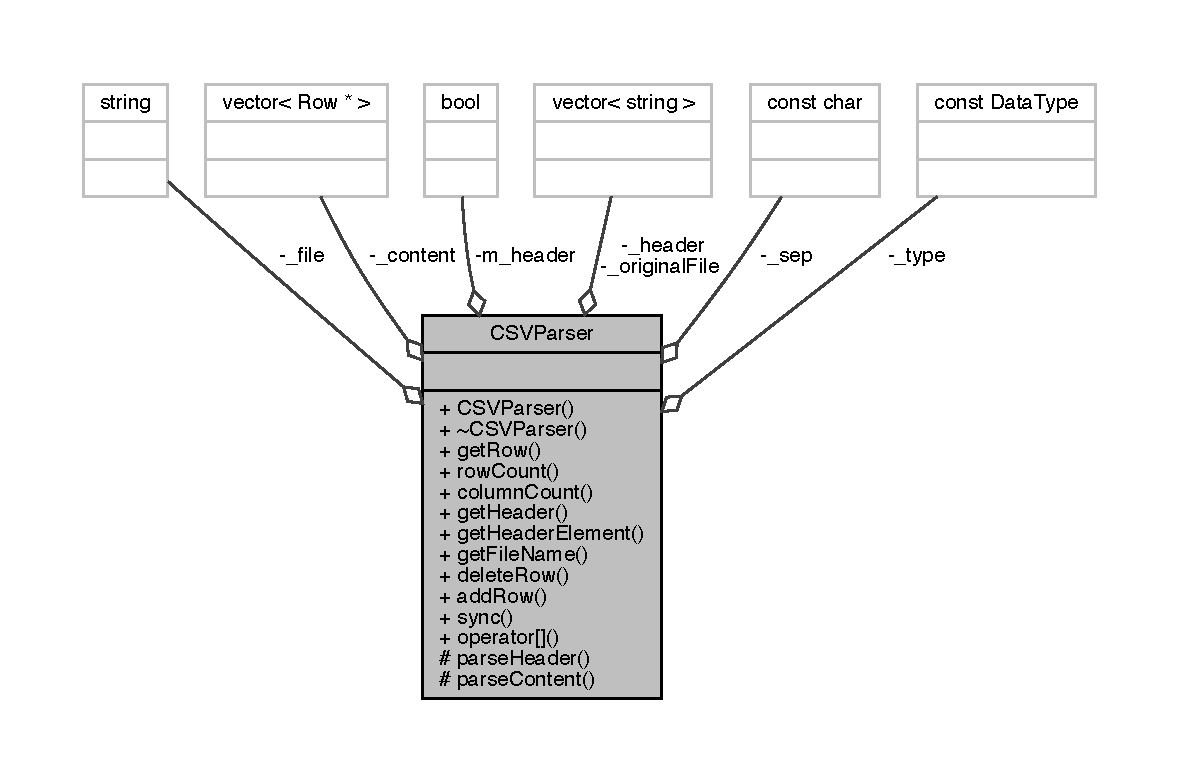
\includegraphics[width=350pt]{class_c_s_v_parser__coll__graph}
\end{center}
\end{figure}
\subsection*{Public Member Functions}
\begin{DoxyCompactItemize}
\item 
\mbox{\hyperlink{class_c_s_v_parser_aba4d9ee88285f39766e7cc810f46d9d9}{C\+S\+V\+Parser}} (const string \&data, const \mbox{\hyperlink{_c_s_vparser_8hpp_ad8ed01ff3ff33333d8e19db4d2818bb6}{Data\+Type}} \&type=\mbox{\hyperlink{_c_s_vparser_8hpp_ad8ed01ff3ff33333d8e19db4d2818bb6a99e2aefa5a03705fd10b8b72e081349f}{e\+F\+I\+LE}}, char sep=\textquotesingle{},\textquotesingle{}, bool has\+Header=true)
\item 
\mbox{\hyperlink{class_c_s_v_parser_a43f06e2e24a260b80e83821c70f91f56}{$\sim$\+C\+S\+V\+Parser}} (void)
\item 
\mbox{\hyperlink{class_row}{Row}} \& \mbox{\hyperlink{class_c_s_v_parser_a93789f318f0abd972860c507b89d4587}{get\+Row}} (unsigned int row) const
\item 
unsigned int \mbox{\hyperlink{class_c_s_v_parser_ab7596d8458539a585908d41638672f4c}{row\+Count}} (void) const
\item 
unsigned int \mbox{\hyperlink{class_c_s_v_parser_a1e30268d574a0c1911de002a893d7a7e}{column\+Count}} (void) const
\item 
vector$<$ string $>$ \mbox{\hyperlink{class_c_s_v_parser_a95b7d4b188facfec7ebab65413f0130b}{get\+Header}} (void) const
\item 
const string \mbox{\hyperlink{class_c_s_v_parser_ad58dc7b467216ecb75f3bea681af3051}{get\+Header\+Element}} (unsigned int pos) const
\item 
const string \& \mbox{\hyperlink{class_c_s_v_parser_ad9a559d1c8de2a7d88a18170c9e11b80}{get\+File\+Name}} (void) const
\item 
bool \mbox{\hyperlink{class_c_s_v_parser_a1bc14d9edecb802c19ad25bd5cab23b3}{delete\+Row}} (unsigned int row)
\item 
bool \mbox{\hyperlink{class_c_s_v_parser_a7e742c5123efa0a49d576776f8832ddb}{add\+Row}} (unsigned int pos, const vector$<$ string $>$ \&r)
\item 
void \mbox{\hyperlink{class_c_s_v_parser_aa0b2494094eb2ce657787ae830b3cc52}{sync}} (void) const
\item 
\mbox{\hyperlink{class_row}{Row}} \& \mbox{\hyperlink{class_c_s_v_parser_a7d3d0c3f994b825aaba25625f0b01612}{operator\mbox{[}$\,$\mbox{]}}} (unsigned int row) const
\end{DoxyCompactItemize}
\subsection*{Protected Member Functions}
\begin{DoxyCompactItemize}
\item 
void \mbox{\hyperlink{class_c_s_v_parser_a8b556e47ecfea188d4c6c630616f5667}{parse\+Header}} (void)
\item 
void \mbox{\hyperlink{class_c_s_v_parser_aa403f7d8238903aa0e046a9a091ab968}{parse\+Content}} (void)
\end{DoxyCompactItemize}
\subsection*{Private Attributes}
\begin{DoxyCompactItemize}
\item 
string \mbox{\hyperlink{class_c_s_v_parser_a1db17c9285f8fdcaed2499747582e4a9}{\+\_\+file}}
\item 
const \mbox{\hyperlink{_c_s_vparser_8hpp_ad8ed01ff3ff33333d8e19db4d2818bb6}{Data\+Type}} \mbox{\hyperlink{class_c_s_v_parser_a27cff8e618160b2685f1e05b8a7da9cf}{\+\_\+type}}
\item 
const char \mbox{\hyperlink{class_c_s_v_parser_a9d778da8bd668d2393d4402ce7eae9cd}{\+\_\+sep}}
\item 
vector$<$ string $>$ \mbox{\hyperlink{class_c_s_v_parser_afa0c154dd897b5ddcbf8364a9df28eeb}{\+\_\+original\+File}}
\item 
vector$<$ string $>$ \mbox{\hyperlink{class_c_s_v_parser_a9b35b0a143febb8fb388769417fa0777}{\+\_\+header}}
\item 
vector$<$ \mbox{\hyperlink{class_row}{Row}} $\ast$ $>$ \mbox{\hyperlink{class_c_s_v_parser_adff6872f7e93cbc10797bac6173671d4}{\+\_\+content}}
\item 
bool \mbox{\hyperlink{class_c_s_v_parser_a4dcb7bb113b65d0abf816dd899395545}{m\+\_\+header}}
\end{DoxyCompactItemize}


\subsection{Detailed Description}
This class is used to read and parse a csv file or to write some values as a csv file. 

\subsection{Constructor \& Destructor Documentation}
\mbox{\Hypertarget{class_c_s_v_parser_aba4d9ee88285f39766e7cc810f46d9d9}\label{class_c_s_v_parser_aba4d9ee88285f39766e7cc810f46d9d9}} 
\index{CSVParser@{CSVParser}!CSVParser@{CSVParser}}
\index{CSVParser@{CSVParser}!CSVParser@{CSVParser}}
\subsubsection{\texorpdfstring{CSVParser()}{CSVParser()}}
{\footnotesize\ttfamily C\+S\+V\+Parser\+::\+C\+S\+V\+Parser (\begin{DoxyParamCaption}\item[{const string \&}]{data,  }\item[{const \mbox{\hyperlink{_c_s_vparser_8hpp_ad8ed01ff3ff33333d8e19db4d2818bb6}{Data\+Type}} \&}]{type = {\ttfamily \mbox{\hyperlink{_c_s_vparser_8hpp_ad8ed01ff3ff33333d8e19db4d2818bb6a99e2aefa5a03705fd10b8b72e081349f}{e\+F\+I\+LE}}},  }\item[{char}]{sep = {\ttfamily \textquotesingle{},\textquotesingle{}},  }\item[{bool}]{has\+Header = {\ttfamily true} }\end{DoxyParamCaption})}

Constructor of the class. It need the name of the csv file, the file type, the separator and a boolean that indicates if the file has header or not. 
\begin{DoxyParams}{Parameters}
{\em data} & the name of the file \\
\hline
{\em type} & the file type\+: could be e\+F\+I\+LE for normal text files or e\+P\+U\+RE if the input is a string \\
\hline
{\em sep} & the separator of the individula values in a line of the csv file \\
\hline
{\em has\+Header} & true means that the csv file has a header line, false that it doesn\textquotesingle{}t have a header \\
\hline
\end{DoxyParams}
\mbox{\Hypertarget{class_c_s_v_parser_a43f06e2e24a260b80e83821c70f91f56}\label{class_c_s_v_parser_a43f06e2e24a260b80e83821c70f91f56}} 
\index{CSVParser@{CSVParser}!````~CSVParser@{$\sim$CSVParser}}
\index{````~CSVParser@{$\sim$CSVParser}!CSVParser@{CSVParser}}
\subsubsection{\texorpdfstring{$\sim$CSVParser()}{~CSVParser()}}
{\footnotesize\ttfamily C\+S\+V\+Parser\+::$\sim$\+C\+S\+V\+Parser (\begin{DoxyParamCaption}\item[{void}]{ }\end{DoxyParamCaption})}

Destructor 

\subsection{Member Function Documentation}
\mbox{\Hypertarget{class_c_s_v_parser_a7e742c5123efa0a49d576776f8832ddb}\label{class_c_s_v_parser_a7e742c5123efa0a49d576776f8832ddb}} 
\index{CSVParser@{CSVParser}!addRow@{addRow}}
\index{addRow@{addRow}!CSVParser@{CSVParser}}
\subsubsection{\texorpdfstring{addRow()}{addRow()}}
{\footnotesize\ttfamily bool C\+S\+V\+Parser\+::add\+Row (\begin{DoxyParamCaption}\item[{unsigned int}]{pos,  }\item[{const vector$<$ string $>$ \&}]{r }\end{DoxyParamCaption})}

Inserts a \mbox{\hyperlink{class_row}{Row}} object at a given position 
\begin{DoxyParams}{Parameters}
{\em pos} & the position where we want to insert the \mbox{\hyperlink{class_row}{Row}} object \\
\hline
{\em r} & a vector containing the values in the \mbox{\hyperlink{class_row}{Row}}. \\
\hline
\end{DoxyParams}
\begin{DoxyReturn}{Returns}
true if the insertion is successful, false otherwise (i.\+e. the pos parameter is outside the limits of the container that stores the Rows of the csv file. 
\end{DoxyReturn}
\mbox{\Hypertarget{class_c_s_v_parser_a1e30268d574a0c1911de002a893d7a7e}\label{class_c_s_v_parser_a1e30268d574a0c1911de002a893d7a7e}} 
\index{CSVParser@{CSVParser}!columnCount@{columnCount}}
\index{columnCount@{columnCount}!CSVParser@{CSVParser}}
\subsubsection{\texorpdfstring{columnCount()}{columnCount()}}
{\footnotesize\ttfamily unsigned int C\+S\+V\+Parser\+::column\+Count (\begin{DoxyParamCaption}\item[{void}]{ }\end{DoxyParamCaption}) const}

Returns the number of the columns of the csv file. \begin{DoxyReturn}{Returns}
the number of the columns of the csv file. 
\end{DoxyReturn}
\mbox{\Hypertarget{class_c_s_v_parser_a1bc14d9edecb802c19ad25bd5cab23b3}\label{class_c_s_v_parser_a1bc14d9edecb802c19ad25bd5cab23b3}} 
\index{CSVParser@{CSVParser}!deleteRow@{deleteRow}}
\index{deleteRow@{deleteRow}!CSVParser@{CSVParser}}
\subsubsection{\texorpdfstring{deleteRow()}{deleteRow()}}
{\footnotesize\ttfamily bool C\+S\+V\+Parser\+::delete\+Row (\begin{DoxyParamCaption}\item[{unsigned int}]{row }\end{DoxyParamCaption})}

Removes a row specified by its number 
\begin{DoxyParams}{Parameters}
{\em row} & the number of the row to be deleted \\
\hline
\end{DoxyParams}
\begin{DoxyReturn}{Returns}
true if the removal succeeded, false otherwise 
\end{DoxyReturn}
\mbox{\Hypertarget{class_c_s_v_parser_ad9a559d1c8de2a7d88a18170c9e11b80}\label{class_c_s_v_parser_ad9a559d1c8de2a7d88a18170c9e11b80}} 
\index{CSVParser@{CSVParser}!getFileName@{getFileName}}
\index{getFileName@{getFileName}!CSVParser@{CSVParser}}
\subsubsection{\texorpdfstring{getFileName()}{getFileName()}}
{\footnotesize\ttfamily const string\& C\+S\+V\+Parser\+::get\+File\+Name (\begin{DoxyParamCaption}\item[{void}]{ }\end{DoxyParamCaption}) const}

Returns the name of the csv file \begin{DoxyReturn}{Returns}
the name of the csv file 
\end{DoxyReturn}
\mbox{\Hypertarget{class_c_s_v_parser_a95b7d4b188facfec7ebab65413f0130b}\label{class_c_s_v_parser_a95b7d4b188facfec7ebab65413f0130b}} 
\index{CSVParser@{CSVParser}!getHeader@{getHeader}}
\index{getHeader@{getHeader}!CSVParser@{CSVParser}}
\subsubsection{\texorpdfstring{getHeader()}{getHeader()}}
{\footnotesize\ttfamily vector$<$string$>$ C\+S\+V\+Parser\+::get\+Header (\begin{DoxyParamCaption}\item[{void}]{ }\end{DoxyParamCaption}) const}

Returns a vector containing the names of the columns as they are specified in the header line of the csv file. \begin{DoxyReturn}{Returns}
a vector containing the names of the columns as they are specified in the header line of the csv file. 
\end{DoxyReturn}
\mbox{\Hypertarget{class_c_s_v_parser_ad58dc7b467216ecb75f3bea681af3051}\label{class_c_s_v_parser_ad58dc7b467216ecb75f3bea681af3051}} 
\index{CSVParser@{CSVParser}!getHeaderElement@{getHeaderElement}}
\index{getHeaderElement@{getHeaderElement}!CSVParser@{CSVParser}}
\subsubsection{\texorpdfstring{getHeaderElement()}{getHeaderElement()}}
{\footnotesize\ttfamily const string C\+S\+V\+Parser\+::get\+Header\+Element (\begin{DoxyParamCaption}\item[{unsigned int}]{pos }\end{DoxyParamCaption}) const}

Returns the name of a specific column given by its position in the header line 
\begin{DoxyParams}{Parameters}
{\em pos} & the number of the column \\
\hline
\end{DoxyParams}
\begin{DoxyReturn}{Returns}
the name of a specific column given by its position in the header line 
\end{DoxyReturn}
\mbox{\Hypertarget{class_c_s_v_parser_a93789f318f0abd972860c507b89d4587}\label{class_c_s_v_parser_a93789f318f0abd972860c507b89d4587}} 
\index{CSVParser@{CSVParser}!getRow@{getRow}}
\index{getRow@{getRow}!CSVParser@{CSVParser}}
\subsubsection{\texorpdfstring{getRow()}{getRow()}}
{\footnotesize\ttfamily \mbox{\hyperlink{class_row}{Row}}\& C\+S\+V\+Parser\+::get\+Row (\begin{DoxyParamCaption}\item[{unsigned int}]{row }\end{DoxyParamCaption}) const}

Returns a \mbox{\hyperlink{class_row}{Row}} object specified by its number in the file 
\begin{DoxyParams}{Parameters}
{\em row} & the number of the line that was used to build the \mbox{\hyperlink{class_row}{Row}} object \\
\hline
\end{DoxyParams}
\begin{DoxyReturn}{Returns}
a \mbox{\hyperlink{class_row}{Row}} object specified by its number in the file 
\end{DoxyReturn}
\mbox{\Hypertarget{class_c_s_v_parser_a7d3d0c3f994b825aaba25625f0b01612}\label{class_c_s_v_parser_a7d3d0c3f994b825aaba25625f0b01612}} 
\index{CSVParser@{CSVParser}!operator\mbox{[}\mbox{]}@{operator[]}}
\index{operator\mbox{[}\mbox{]}@{operator[]}!CSVParser@{CSVParser}}
\subsubsection{\texorpdfstring{operator[]()}{operator[]()}}
{\footnotesize\ttfamily \mbox{\hyperlink{class_row}{Row}}\& C\+S\+V\+Parser\+::operator\mbox{[}$\,$\mbox{]} (\begin{DoxyParamCaption}\item[{unsigned int}]{row }\end{DoxyParamCaption}) const}

Overloaded operator 
\begin{DoxyParams}{Parameters}
{\em row} & the number of the row to be retrieved \\
\hline
\end{DoxyParams}
\begin{DoxyReturn}{Returns}
the \mbox{\hyperlink{class_row}{Row}} object at the position specified by row 
\end{DoxyReturn}
\mbox{\Hypertarget{class_c_s_v_parser_aa403f7d8238903aa0e046a9a091ab968}\label{class_c_s_v_parser_aa403f7d8238903aa0e046a9a091ab968}} 
\index{CSVParser@{CSVParser}!parseContent@{parseContent}}
\index{parseContent@{parseContent}!CSVParser@{CSVParser}}
\subsubsection{\texorpdfstring{parseContent()}{parseContent()}}
{\footnotesize\ttfamily void C\+S\+V\+Parser\+::parse\+Content (\begin{DoxyParamCaption}\item[{void}]{ }\end{DoxyParamCaption})\hspace{0.3cm}{\ttfamily [protected]}}

\mbox{\Hypertarget{class_c_s_v_parser_a8b556e47ecfea188d4c6c630616f5667}\label{class_c_s_v_parser_a8b556e47ecfea188d4c6c630616f5667}} 
\index{CSVParser@{CSVParser}!parseHeader@{parseHeader}}
\index{parseHeader@{parseHeader}!CSVParser@{CSVParser}}
\subsubsection{\texorpdfstring{parseHeader()}{parseHeader()}}
{\footnotesize\ttfamily void C\+S\+V\+Parser\+::parse\+Header (\begin{DoxyParamCaption}\item[{void}]{ }\end{DoxyParamCaption})\hspace{0.3cm}{\ttfamily [protected]}}

\mbox{\Hypertarget{class_c_s_v_parser_ab7596d8458539a585908d41638672f4c}\label{class_c_s_v_parser_ab7596d8458539a585908d41638672f4c}} 
\index{CSVParser@{CSVParser}!rowCount@{rowCount}}
\index{rowCount@{rowCount}!CSVParser@{CSVParser}}
\subsubsection{\texorpdfstring{rowCount()}{rowCount()}}
{\footnotesize\ttfamily unsigned int C\+S\+V\+Parser\+::row\+Count (\begin{DoxyParamCaption}\item[{void}]{ }\end{DoxyParamCaption}) const}

Returns the number of lines in the csv file without counting the header line, if it exists \begin{DoxyReturn}{Returns}
the number of lines in the csv file without counting the header line, if it exists 
\end{DoxyReturn}
\mbox{\Hypertarget{class_c_s_v_parser_aa0b2494094eb2ce657787ae830b3cc52}\label{class_c_s_v_parser_aa0b2494094eb2ce657787ae830b3cc52}} 
\index{CSVParser@{CSVParser}!sync@{sync}}
\index{sync@{sync}!CSVParser@{CSVParser}}
\subsubsection{\texorpdfstring{sync()}{sync()}}
{\footnotesize\ttfamily void C\+S\+V\+Parser\+::sync (\begin{DoxyParamCaption}\item[{void}]{ }\end{DoxyParamCaption}) const}

Flushes the content to a file on disk and then closes the file. 

\subsection{Member Data Documentation}
\mbox{\Hypertarget{class_c_s_v_parser_adff6872f7e93cbc10797bac6173671d4}\label{class_c_s_v_parser_adff6872f7e93cbc10797bac6173671d4}} 
\index{CSVParser@{CSVParser}!\_content@{\_content}}
\index{\_content@{\_content}!CSVParser@{CSVParser}}
\subsubsection{\texorpdfstring{\_content}{\_content}}
{\footnotesize\ttfamily vector$<$\mbox{\hyperlink{class_row}{Row}} $\ast$$>$ C\+S\+V\+Parser\+::\+\_\+content\hspace{0.3cm}{\ttfamily [private]}}

\mbox{\Hypertarget{class_c_s_v_parser_a1db17c9285f8fdcaed2499747582e4a9}\label{class_c_s_v_parser_a1db17c9285f8fdcaed2499747582e4a9}} 
\index{CSVParser@{CSVParser}!\_file@{\_file}}
\index{\_file@{\_file}!CSVParser@{CSVParser}}
\subsubsection{\texorpdfstring{\_file}{\_file}}
{\footnotesize\ttfamily string C\+S\+V\+Parser\+::\+\_\+file\hspace{0.3cm}{\ttfamily [private]}}

\mbox{\Hypertarget{class_c_s_v_parser_a9b35b0a143febb8fb388769417fa0777}\label{class_c_s_v_parser_a9b35b0a143febb8fb388769417fa0777}} 
\index{CSVParser@{CSVParser}!\_header@{\_header}}
\index{\_header@{\_header}!CSVParser@{CSVParser}}
\subsubsection{\texorpdfstring{\_header}{\_header}}
{\footnotesize\ttfamily vector$<$string$>$ C\+S\+V\+Parser\+::\+\_\+header\hspace{0.3cm}{\ttfamily [private]}}

\mbox{\Hypertarget{class_c_s_v_parser_afa0c154dd897b5ddcbf8364a9df28eeb}\label{class_c_s_v_parser_afa0c154dd897b5ddcbf8364a9df28eeb}} 
\index{CSVParser@{CSVParser}!\_originalFile@{\_originalFile}}
\index{\_originalFile@{\_originalFile}!CSVParser@{CSVParser}}
\subsubsection{\texorpdfstring{\_originalFile}{\_originalFile}}
{\footnotesize\ttfamily vector$<$string$>$ C\+S\+V\+Parser\+::\+\_\+original\+File\hspace{0.3cm}{\ttfamily [private]}}

\mbox{\Hypertarget{class_c_s_v_parser_a9d778da8bd668d2393d4402ce7eae9cd}\label{class_c_s_v_parser_a9d778da8bd668d2393d4402ce7eae9cd}} 
\index{CSVParser@{CSVParser}!\_sep@{\_sep}}
\index{\_sep@{\_sep}!CSVParser@{CSVParser}}
\subsubsection{\texorpdfstring{\_sep}{\_sep}}
{\footnotesize\ttfamily const char C\+S\+V\+Parser\+::\+\_\+sep\hspace{0.3cm}{\ttfamily [private]}}

\mbox{\Hypertarget{class_c_s_v_parser_a27cff8e618160b2685f1e05b8a7da9cf}\label{class_c_s_v_parser_a27cff8e618160b2685f1e05b8a7da9cf}} 
\index{CSVParser@{CSVParser}!\_type@{\_type}}
\index{\_type@{\_type}!CSVParser@{CSVParser}}
\subsubsection{\texorpdfstring{\_type}{\_type}}
{\footnotesize\ttfamily const \mbox{\hyperlink{_c_s_vparser_8hpp_ad8ed01ff3ff33333d8e19db4d2818bb6}{Data\+Type}} C\+S\+V\+Parser\+::\+\_\+type\hspace{0.3cm}{\ttfamily [private]}}

\mbox{\Hypertarget{class_c_s_v_parser_a4dcb7bb113b65d0abf816dd899395545}\label{class_c_s_v_parser_a4dcb7bb113b65d0abf816dd899395545}} 
\index{CSVParser@{CSVParser}!m\_header@{m\_header}}
\index{m\_header@{m\_header}!CSVParser@{CSVParser}}
\subsubsection{\texorpdfstring{m\_header}{m\_header}}
{\footnotesize\ttfamily bool C\+S\+V\+Parser\+::m\+\_\+header\hspace{0.3cm}{\ttfamily [private]}}



The documentation for this class was generated from the following file\+:\begin{DoxyCompactItemize}
\item 
include/\mbox{\hyperlink{_c_s_vparser_8hpp}{C\+S\+Vparser.\+hpp}}\end{DoxyCompactItemize}

\input{class_displace}
\hypertarget{class_e_m_field}{}\section{E\+M\+Field Class Reference}
\label{class_e_m_field}\index{EMField@{EMField}}


{\ttfamily \#include $<$E\+M\+Field.\+h$>$}



Collaboration diagram for E\+M\+Field\+:\nopagebreak
\begin{figure}[H]
\begin{center}
\leavevmode
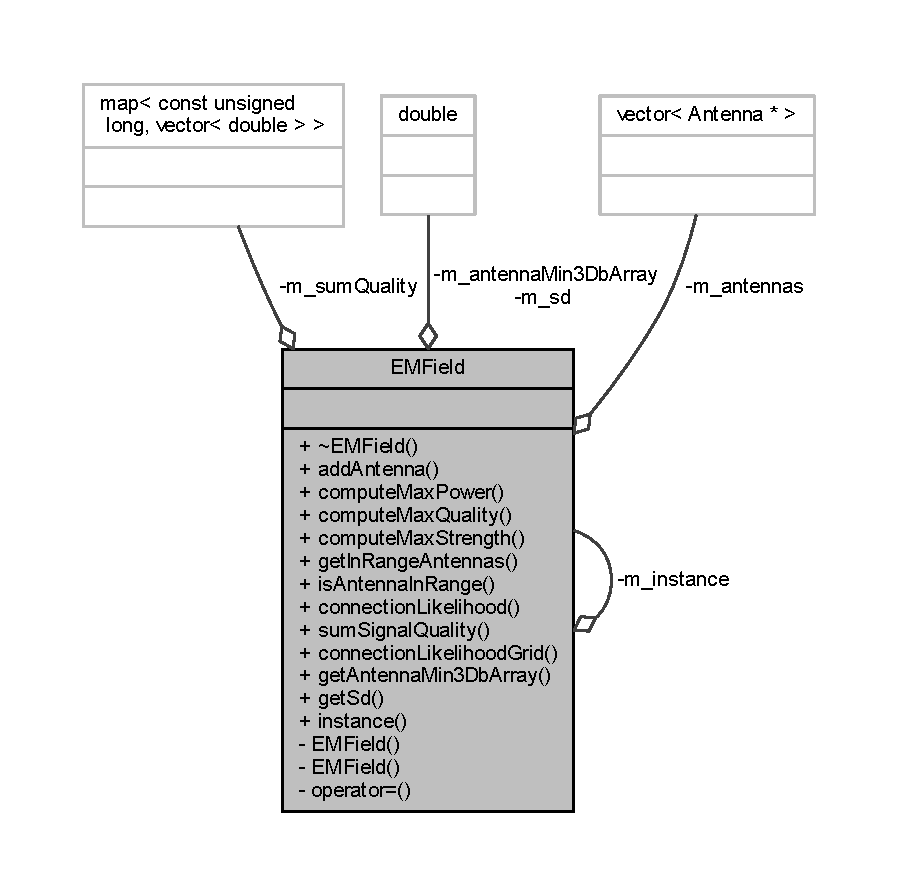
\includegraphics[width=350pt]{class_e_m_field__coll__graph}
\end{center}
\end{figure}
\subsection*{Public Member Functions}
\begin{DoxyCompactItemize}
\item 
virtual \mbox{\hyperlink{class_e_m_field_abe7db07a27a120858107d5efa5f14edb}{$\sim$\+E\+M\+Field}} ()
\item 
void \mbox{\hyperlink{class_e_m_field_ac531ecbce4c81aa5da19fe3c734a585c}{add\+Antenna}} (\mbox{\hyperlink{class_antenna}{Antenna}} $\ast$a)
\item 
pair$<$ \mbox{\hyperlink{class_antenna}{Antenna}} $\ast$, double $>$ \mbox{\hyperlink{class_e_m_field_a01cfb9fea3dadfcfe5d6f00551193acd}{compute\+Max\+Power}} (const Point $\ast$p, const unsigned long mno\+Id)
\item 
pair$<$ \mbox{\hyperlink{class_antenna}{Antenna}} $\ast$, double $>$ \mbox{\hyperlink{class_e_m_field_ac866f6224e34895a0ee085c4baf43a01}{compute\+Max\+Quality}} (const Point $\ast$p, const unsigned long mno\+Id)
\item 
pair$<$ \mbox{\hyperlink{class_antenna}{Antenna}} $\ast$, double $>$ \mbox{\hyperlink{class_e_m_field_a9a3cdbca4fcf408ce58a30fb98de1bbb}{compute\+Max\+Strength}} (const Point $\ast$p, const unsigned long mno\+Id)
\item 
vector$<$ pair$<$ \mbox{\hyperlink{class_antenna}{Antenna}} $\ast$, double $>$ $>$ \mbox{\hyperlink{class_e_m_field_a2ad800417b06a62e68edd1fccb5c4b93}{get\+In\+Range\+Antennas}} (const Point $\ast$p, const double threshold, const \mbox{\hyperlink{class_holdable_agent_ae2c334b004d7b9c5a999cf2618e4e518}{Holdable\+Agent\+::\+C\+O\+N\+N\+E\+C\+T\+I\+O\+N\+\_\+\+T\+Y\+PE}} conn\+Type, unsigned long mno\+Id)
\item 
bool \mbox{\hyperlink{class_e_m_field_a5cd43aded41779d2d24de3f3e5c717d0}{is\+Antenna\+In\+Range}} (const Point $\ast$p, \mbox{\hyperlink{class_antenna}{Antenna}} $\ast$a, const double threshold, const \mbox{\hyperlink{class_holdable_agent_ae2c334b004d7b9c5a999cf2618e4e518}{Holdable\+Agent\+::\+C\+O\+N\+N\+E\+C\+T\+I\+O\+N\+\_\+\+T\+Y\+PE}} conn\+Type)
\item 
double \mbox{\hyperlink{class_e_m_field_a710da64db53718cdeed7b8c8dc11bba3}{connection\+Likelihood}} (\mbox{\hyperlink{class_antenna}{Antenna}} $\ast$a, const Point $\ast$p)
\item 
vector$<$ double $>$ \mbox{\hyperlink{class_e_m_field_a4995bf4b93c09f12b7aab64c7eb24603}{sum\+Signal\+Quality}} (const \mbox{\hyperlink{class_grid}{Grid}} $\ast$grid, const unsigned long mno\+ID)
\item 
double \mbox{\hyperlink{class_e_m_field_a533effeee35a80746ea7e3ddc5998e48}{connection\+Likelihood\+Grid}} (\mbox{\hyperlink{class_antenna}{Antenna}} $\ast$a, const \mbox{\hyperlink{class_grid}{Grid}} $\ast$g, unsigned long tile\+Index)
\item 
const double $\ast$ \mbox{\hyperlink{class_e_m_field_ab2132484b9c52f2224bc81f354b24df6}{get\+Antenna\+Min3\+Db\+Array}} () const
\item 
double $\ast$ \mbox{\hyperlink{class_e_m_field_a0fea003948a67df01174480480376169}{get\+Sd}} () const
\end{DoxyCompactItemize}
\subsection*{Static Public Member Functions}
\begin{DoxyCompactItemize}
\item 
static \mbox{\hyperlink{class_e_m_field}{E\+M\+Field}} $\ast$ \mbox{\hyperlink{class_e_m_field_acbadbede116ac320398cbfcd19e90ec7}{instance}} ()
\end{DoxyCompactItemize}
\subsection*{Private Member Functions}
\begin{DoxyCompactItemize}
\item 
\mbox{\hyperlink{class_e_m_field_a054f389cfa853008f32c02d874aa4d58}{E\+M\+Field}} ()
\item 
\mbox{\hyperlink{class_e_m_field_a7760631ded36ba2c5a918c97a1cc93e9}{E\+M\+Field}} (const \mbox{\hyperlink{class_e_m_field}{E\+M\+Field}} \&)
\item 
\mbox{\hyperlink{class_e_m_field}{E\+M\+Field}} \& \mbox{\hyperlink{class_e_m_field_ad35e4754cad2016d7df1b8ac45540b35}{operator=}} (const \mbox{\hyperlink{class_e_m_field}{E\+M\+Field}} \&)
\end{DoxyCompactItemize}
\subsection*{Private Attributes}
\begin{DoxyCompactItemize}
\item 
vector$<$ \mbox{\hyperlink{class_antenna}{Antenna}} $\ast$ $>$ \mbox{\hyperlink{class_e_m_field_ab74a3bde70b66fd033bde6c25345a755}{m\+\_\+antennas}}
\item 
map$<$ const unsigned long, vector$<$ double $>$ $>$ \mbox{\hyperlink{class_e_m_field_a18e5a4d972d888c5da458e30e426c7ae}{m\+\_\+sum\+Quality}}
\item 
double $\ast$ \mbox{\hyperlink{class_e_m_field_a96c4c7bc39c2f8afea0dca3280fe145c}{m\+\_\+antenna\+Min3\+Db\+Array}}
\item 
double $\ast$ \mbox{\hyperlink{class_e_m_field_ac2142eafd5b82e43437a8047565f619c}{m\+\_\+sd}}
\end{DoxyCompactItemize}
\subsection*{Static Private Attributes}
\begin{DoxyCompactItemize}
\item 
static \mbox{\hyperlink{class_e_m_field}{E\+M\+Field}} $\ast$ \mbox{\hyperlink{class_e_m_field_a3a75e412fa15cfab78ce64dfbb8af52d}{m\+\_\+instance}}
\end{DoxyCompactItemize}


\subsection{Detailed Description}
This utility singleton class is used to compute different measures of the electromagnetic field radiated by an antenna (power, signal strength etc) and it also provides methods needed to decide to which antenna a mobile device connects. 

\subsection{Constructor \& Destructor Documentation}
\mbox{\Hypertarget{class_e_m_field_abe7db07a27a120858107d5efa5f14edb}\label{class_e_m_field_abe7db07a27a120858107d5efa5f14edb}} 
\index{EMField@{EMField}!````~EMField@{$\sim$EMField}}
\index{````~EMField@{$\sim$EMField}!EMField@{EMField}}
\subsubsection{\texorpdfstring{$\sim$EMField()}{~EMField()}}
{\footnotesize\ttfamily virtual E\+M\+Field\+::$\sim$\+E\+M\+Field (\begin{DoxyParamCaption}{ }\end{DoxyParamCaption})\hspace{0.3cm}{\ttfamily [virtual]}}

Default destructor. \mbox{\Hypertarget{class_e_m_field_a054f389cfa853008f32c02d874aa4d58}\label{class_e_m_field_a054f389cfa853008f32c02d874aa4d58}} 
\index{EMField@{EMField}!EMField@{EMField}}
\index{EMField@{EMField}!EMField@{EMField}}
\subsubsection{\texorpdfstring{EMField()}{EMField()}\hspace{0.1cm}{\footnotesize\ttfamily [1/2]}}
{\footnotesize\ttfamily E\+M\+Field\+::\+E\+M\+Field (\begin{DoxyParamCaption}{ }\end{DoxyParamCaption})\hspace{0.3cm}{\ttfamily [private]}}

\mbox{\Hypertarget{class_e_m_field_a7760631ded36ba2c5a918c97a1cc93e9}\label{class_e_m_field_a7760631ded36ba2c5a918c97a1cc93e9}} 
\index{EMField@{EMField}!EMField@{EMField}}
\index{EMField@{EMField}!EMField@{EMField}}
\subsubsection{\texorpdfstring{EMField()}{EMField()}\hspace{0.1cm}{\footnotesize\ttfamily [2/2]}}
{\footnotesize\ttfamily E\+M\+Field\+::\+E\+M\+Field (\begin{DoxyParamCaption}\item[{const \mbox{\hyperlink{class_e_m_field}{E\+M\+Field}} \&}]{ }\end{DoxyParamCaption})\hspace{0.3cm}{\ttfamily [private]}}



\subsection{Member Function Documentation}
\mbox{\Hypertarget{class_e_m_field_ac531ecbce4c81aa5da19fe3c734a585c}\label{class_e_m_field_ac531ecbce4c81aa5da19fe3c734a585c}} 
\index{EMField@{EMField}!addAntenna@{addAntenna}}
\index{addAntenna@{addAntenna}!EMField@{EMField}}
\subsubsection{\texorpdfstring{addAntenna()}{addAntenna()}}
{\footnotesize\ttfamily void E\+M\+Field\+::add\+Antenna (\begin{DoxyParamCaption}\item[{\mbox{\hyperlink{class_antenna}{Antenna}} $\ast$}]{a }\end{DoxyParamCaption})}

Add a pointer to an \mbox{\hyperlink{class_antenna}{Antenna}} object to an internal collection needed for computations. Although these pointers are kept in an Agent\+Collection object they are also added to a local vector in this class for performance reasons. 
\begin{DoxyParams}{Parameters}
{\em a} & a pointer to the \mbox{\hyperlink{class_antenna}{Antenna}} object \\
\hline
\end{DoxyParams}
\mbox{\Hypertarget{class_e_m_field_a01cfb9fea3dadfcfe5d6f00551193acd}\label{class_e_m_field_a01cfb9fea3dadfcfe5d6f00551193acd}} 
\index{EMField@{EMField}!computeMaxPower@{computeMaxPower}}
\index{computeMaxPower@{computeMaxPower}!EMField@{EMField}}
\subsubsection{\texorpdfstring{computeMaxPower()}{computeMaxPower()}}
{\footnotesize\ttfamily pair$<$\mbox{\hyperlink{class_antenna}{Antenna}}$\ast$, double$>$ E\+M\+Field\+::compute\+Max\+Power (\begin{DoxyParamCaption}\item[{const Point $\ast$}]{p,  }\item[{const unsigned long}]{mno\+Id }\end{DoxyParamCaption})}

Returns a pair made of a pointer to an \mbox{\hyperlink{class_antenna}{Antenna}} object and its power with the property that in the location specified by parameter p, the \mbox{\hyperlink{class_antenna}{Antenna}} returned by this method provides the highest power (the power of the field is considered to decrease according a power-\/law). 
\begin{DoxyParams}{Parameters}
{\em p} & the location where we want to find which \mbox{\hyperlink{class_antenna}{Antenna}} provides the highest power the of electromagnetic field. \\
\hline
{\em mno\+Id} & the id of the M\+NO for which we compute the power. Only antennas belonging to this M\+NO will be considered during computations. \\
\hline
\end{DoxyParams}
\begin{DoxyReturn}{Returns}
a pair$<$\+Antenna$\ast$, double$>$ containing a pointer to the \mbox{\hyperlink{class_antenna}{Antenna}} object that provides the highest power of the field in the location specified by p. 
\end{DoxyReturn}
\mbox{\Hypertarget{class_e_m_field_ac866f6224e34895a0ee085c4baf43a01}\label{class_e_m_field_ac866f6224e34895a0ee085c4baf43a01}} 
\index{EMField@{EMField}!computeMaxQuality@{computeMaxQuality}}
\index{computeMaxQuality@{computeMaxQuality}!EMField@{EMField}}
\subsubsection{\texorpdfstring{computeMaxQuality()}{computeMaxQuality()}}
{\footnotesize\ttfamily pair$<$\mbox{\hyperlink{class_antenna}{Antenna}}$\ast$, double$>$ E\+M\+Field\+::compute\+Max\+Quality (\begin{DoxyParamCaption}\item[{const Point $\ast$}]{p,  }\item[{const unsigned long}]{mno\+Id }\end{DoxyParamCaption})}

Returns a pair made of a pointer to an \mbox{\hyperlink{class_antenna}{Antenna}} object and its signal quality with the property that in the location specified by p, the \mbox{\hyperlink{class_antenna}{Antenna}} returned by this method provides signal with the highest quality. The signal quality in this pair is the computed in location given by p. 
\begin{DoxyParams}{Parameters}
{\em p} & indicates the location where we want to find which \mbox{\hyperlink{class_antenna}{Antenna}} provides the highest quality of the signal. \\
\hline
{\em mno\+Id} & the id of the M\+NO for which we compute the signal quality. Only antennas belonging to this M\+NO will be considered during computations. \\
\hline
\end{DoxyParams}
\begin{DoxyReturn}{Returns}
a pair$<$\+Antenna$\ast$, double$>$ containing a pointer to the \mbox{\hyperlink{class_antenna}{Antenna}} object that provides a signal with the highest quality in location given by p. 
\end{DoxyReturn}
\mbox{\Hypertarget{class_e_m_field_a9a3cdbca4fcf408ce58a30fb98de1bbb}\label{class_e_m_field_a9a3cdbca4fcf408ce58a30fb98de1bbb}} 
\index{EMField@{EMField}!computeMaxStrength@{computeMaxStrength}}
\index{computeMaxStrength@{computeMaxStrength}!EMField@{EMField}}
\subsubsection{\texorpdfstring{computeMaxStrength()}{computeMaxStrength()}}
{\footnotesize\ttfamily pair$<$\mbox{\hyperlink{class_antenna}{Antenna}}$\ast$, double$>$ E\+M\+Field\+::compute\+Max\+Strength (\begin{DoxyParamCaption}\item[{const Point $\ast$}]{p,  }\item[{const unsigned long}]{mno\+Id }\end{DoxyParamCaption})}

Returns a pair made of a pointer to an \mbox{\hyperlink{class_antenna}{Antenna}} object and its signal strength with the property that in the location specified by p, the \mbox{\hyperlink{class_antenna}{Antenna}} returned by this method provides signal with the highest strength. The signal strength in this pair is the computed in location given by p. 
\begin{DoxyParams}{Parameters}
{\em p} & indicates the location where we want to find which \mbox{\hyperlink{class_antenna}{Antenna}} provides the highest strength of the signal. \\
\hline
{\em mno\+Id} & the id of the M\+NO for which we compute the signal strength. Only antennas belonging to this M\+NO will be considered during computations. \\
\hline
\end{DoxyParams}
\begin{DoxyReturn}{Returns}
a pair$<$\+Antenna$\ast$, double$>$ containing a pointer to the \mbox{\hyperlink{class_antenna}{Antenna}} object that provides a signal with the highest strength in location given by p. 
\end{DoxyReturn}
\mbox{\Hypertarget{class_e_m_field_a710da64db53718cdeed7b8c8dc11bba3}\label{class_e_m_field_a710da64db53718cdeed7b8c8dc11bba3}} 
\index{EMField@{EMField}!connectionLikelihood@{connectionLikelihood}}
\index{connectionLikelihood@{connectionLikelihood}!EMField@{EMField}}
\subsubsection{\texorpdfstring{connectionLikelihood()}{connectionLikelihood()}}
{\footnotesize\ttfamily double E\+M\+Field\+::connection\+Likelihood (\begin{DoxyParamCaption}\item[{\mbox{\hyperlink{class_antenna}{Antenna}} $\ast$}]{a,  }\item[{const Point $\ast$}]{p }\end{DoxyParamCaption})}

Computes the connection likelihood for \mbox{\hyperlink{class_antenna}{Antenna}} indicated by a in a certain location given by p. The connection likelihood is computed dividing the signal quality provided by \mbox{\hyperlink{class_antenna}{Antenna}} indicated through p by the sum of the signal quality provided by all antennas of an M\+NO. 
\begin{DoxyParams}{Parameters}
{\em a} & a pointer to an \mbox{\hyperlink{class_antenna}{Antenna}} object. \\
\hline
{\em p} & a location in space. \\
\hline
\end{DoxyParams}
\begin{DoxyReturn}{Returns}
the connection likelihood for \mbox{\hyperlink{class_antenna}{Antenna}} a in location p. 
\end{DoxyReturn}
\mbox{\Hypertarget{class_e_m_field_a533effeee35a80746ea7e3ddc5998e48}\label{class_e_m_field_a533effeee35a80746ea7e3ddc5998e48}} 
\index{EMField@{EMField}!connectionLikelihoodGrid@{connectionLikelihoodGrid}}
\index{connectionLikelihoodGrid@{connectionLikelihoodGrid}!EMField@{EMField}}
\subsubsection{\texorpdfstring{connectionLikelihoodGrid()}{connectionLikelihoodGrid()}}
{\footnotesize\ttfamily double E\+M\+Field\+::connection\+Likelihood\+Grid (\begin{DoxyParamCaption}\item[{\mbox{\hyperlink{class_antenna}{Antenna}} $\ast$}]{a,  }\item[{const \mbox{\hyperlink{class_grid}{Grid}} $\ast$}]{g,  }\item[{unsigned long}]{tile\+Index }\end{DoxyParamCaption})}

Computes the connection likelihood for \mbox{\hyperlink{class_antenna}{Antenna}} indicated by a in the center of the tile indicated by tile\+Index 
\begin{DoxyParams}{Parameters}
{\em a} & a pointer to an \mbox{\hyperlink{class_antenna}{Antenna}} object. \\
\hline
{\em g} & a pointer to the reference \mbox{\hyperlink{class_grid}{Grid}} object \\
\hline
{\em tile\+Index} & the index of the tile where we want to compute the connection likelihood. \\
\hline
\end{DoxyParams}
\begin{DoxyReturn}{Returns}
the connection likelihood for \mbox{\hyperlink{class_antenna}{Antenna}} a in the center of the tile with the index tile\+Index. 
\end{DoxyReturn}
\mbox{\Hypertarget{class_e_m_field_ab2132484b9c52f2224bc81f354b24df6}\label{class_e_m_field_ab2132484b9c52f2224bc81f354b24df6}} 
\index{EMField@{EMField}!getAntennaMin3DbArray@{getAntennaMin3DbArray}}
\index{getAntennaMin3DbArray@{getAntennaMin3DbArray}!EMField@{EMField}}
\subsubsection{\texorpdfstring{getAntennaMin3DbArray()}{getAntennaMin3DbArray()}}
{\footnotesize\ttfamily const double$\ast$ E\+M\+Field\+::get\+Antenna\+Min3\+Db\+Array (\begin{DoxyParamCaption}{ }\end{DoxyParamCaption}) const}

\mbox{\Hypertarget{class_e_m_field_a2ad800417b06a62e68edd1fccb5c4b93}\label{class_e_m_field_a2ad800417b06a62e68edd1fccb5c4b93}} 
\index{EMField@{EMField}!getInRangeAntennas@{getInRangeAntennas}}
\index{getInRangeAntennas@{getInRangeAntennas}!EMField@{EMField}}
\subsubsection{\texorpdfstring{getInRangeAntennas()}{getInRangeAntennas()}}
{\footnotesize\ttfamily vector$<$pair$<$\mbox{\hyperlink{class_antenna}{Antenna}}$\ast$, double$>$ $>$ E\+M\+Field\+::get\+In\+Range\+Antennas (\begin{DoxyParamCaption}\item[{const Point $\ast$}]{p,  }\item[{const double}]{threshold,  }\item[{const \mbox{\hyperlink{class_holdable_agent_ae2c334b004d7b9c5a999cf2618e4e518}{Holdable\+Agent\+::\+C\+O\+N\+N\+E\+C\+T\+I\+O\+N\+\_\+\+T\+Y\+PE}}}]{conn\+Type,  }\item[{unsigned long}]{mno\+Id }\end{DoxyParamCaption})}

Returns a vector of pairs made up of a pointer to an \mbox{\hyperlink{class_antenna}{Antenna}} object and its power, signal quality or signal strength. All the antennas in this vector provides a signal with a power or signal quality greater than the threshold provided as threshold, i.\+e. this vector contains all antennas that have in their coverage area the location given by point p. 
\begin{DoxyParams}{Parameters}
{\em p} & the location where we want to have the list with the all antennas that covers it. \\
\hline
{\em threshold} & the lowest limit of the power or signal quality below which the signal is considered to be only noise, i.\+e. it defines the limit of the coverage area. \\
\hline
{\em conn\+Type} & indicates the mechanism used to set up a connection between an antenna and a mobile phone \\
\hline
{\em mno\+Id} & the id of the M\+NO for which we build the resulting vector. Only antennas belonging to this M\+NO will be considered during computations. \\
\hline
\end{DoxyParams}
\begin{DoxyReturn}{Returns}
a vector of pairs made up of a pointer to an \mbox{\hyperlink{class_antenna}{Antenna}} object and its power, signal quality or signal strength, according to the value of the conn\+Type. All the antennas in this vector provides a signal with a power, signal quality or signal strength greater than the threshold. 
\end{DoxyReturn}
\mbox{\Hypertarget{class_e_m_field_a0fea003948a67df01174480480376169}\label{class_e_m_field_a0fea003948a67df01174480480376169}} 
\index{EMField@{EMField}!getSd@{getSd}}
\index{getSd@{getSd}!EMField@{EMField}}
\subsubsection{\texorpdfstring{getSd()}{getSd()}}
{\footnotesize\ttfamily double$\ast$ E\+M\+Field\+::get\+Sd (\begin{DoxyParamCaption}{ }\end{DoxyParamCaption}) const}

\mbox{\Hypertarget{class_e_m_field_acbadbede116ac320398cbfcd19e90ec7}\label{class_e_m_field_acbadbede116ac320398cbfcd19e90ec7}} 
\index{EMField@{EMField}!instance@{instance}}
\index{instance@{instance}!EMField@{EMField}}
\subsubsection{\texorpdfstring{instance()}{instance()}}
{\footnotesize\ttfamily static \mbox{\hyperlink{class_e_m_field}{E\+M\+Field}}$\ast$ E\+M\+Field\+::instance (\begin{DoxyParamCaption}{ }\end{DoxyParamCaption})\hspace{0.3cm}{\ttfamily [inline]}, {\ttfamily [static]}}

Returns an instance of this class. This class is a singleton. \begin{DoxyReturn}{Returns}
an instance of this class. 
\end{DoxyReturn}
\mbox{\Hypertarget{class_e_m_field_a5cd43aded41779d2d24de3f3e5c717d0}\label{class_e_m_field_a5cd43aded41779d2d24de3f3e5c717d0}} 
\index{EMField@{EMField}!isAntennaInRange@{isAntennaInRange}}
\index{isAntennaInRange@{isAntennaInRange}!EMField@{EMField}}
\subsubsection{\texorpdfstring{isAntennaInRange()}{isAntennaInRange()}}
{\footnotesize\ttfamily bool E\+M\+Field\+::is\+Antenna\+In\+Range (\begin{DoxyParamCaption}\item[{const Point $\ast$}]{p,  }\item[{\mbox{\hyperlink{class_antenna}{Antenna}} $\ast$}]{a,  }\item[{const double}]{threshold,  }\item[{const \mbox{\hyperlink{class_holdable_agent_ae2c334b004d7b9c5a999cf2618e4e518}{Holdable\+Agent\+::\+C\+O\+N\+N\+E\+C\+T\+I\+O\+N\+\_\+\+T\+Y\+PE}}}]{conn\+Type }\end{DoxyParamCaption})}

Checks if p is in the coverage area of \mbox{\hyperlink{class_antenna}{Antenna}} pointed out by a. The coverage area is considered the area where the signal quality or the power of the field is greater than the value of threshold. 
\begin{DoxyParams}{Parameters}
{\em p} & the location that we want to check the power or the quality of the signal \\
\hline
{\em a} & pointer to an \mbox{\hyperlink{class_antenna}{Antenna}} object for which we want to check if it covers the point p. \\
\hline
{\em threshold} & the lower limit of the power or signal quality below which the signal is considered only noise. \\
\hline
{\em conn\+Type} & indicates the mechanism used to set up a connection between an antenna and a mobile phone. \\
\hline
\end{DoxyParams}
\begin{DoxyReturn}{Returns}
true is the \mbox{\hyperlink{class_antenna}{Antenna}} object provide enough power or signal quality in the location given as p. 
\end{DoxyReturn}
\mbox{\Hypertarget{class_e_m_field_ad35e4754cad2016d7df1b8ac45540b35}\label{class_e_m_field_ad35e4754cad2016d7df1b8ac45540b35}} 
\index{EMField@{EMField}!operator=@{operator=}}
\index{operator=@{operator=}!EMField@{EMField}}
\subsubsection{\texorpdfstring{operator=()}{operator=()}}
{\footnotesize\ttfamily \mbox{\hyperlink{class_e_m_field}{E\+M\+Field}}\& E\+M\+Field\+::operator= (\begin{DoxyParamCaption}\item[{const \mbox{\hyperlink{class_e_m_field}{E\+M\+Field}} \&}]{ }\end{DoxyParamCaption})\hspace{0.3cm}{\ttfamily [private]}}

\mbox{\Hypertarget{class_e_m_field_a4995bf4b93c09f12b7aab64c7eb24603}\label{class_e_m_field_a4995bf4b93c09f12b7aab64c7eb24603}} 
\index{EMField@{EMField}!sumSignalQuality@{sumSignalQuality}}
\index{sumSignalQuality@{sumSignalQuality}!EMField@{EMField}}
\subsubsection{\texorpdfstring{sumSignalQuality()}{sumSignalQuality()}}
{\footnotesize\ttfamily vector$<$double$>$ E\+M\+Field\+::sum\+Signal\+Quality (\begin{DoxyParamCaption}\item[{const \mbox{\hyperlink{class_grid}{Grid}} $\ast$}]{grid,  }\item[{const unsigned long}]{mno\+ID }\end{DoxyParamCaption})}

Computes the sum of the signal quality given by all antennas belonging to an M\+NO for all tiles in the reference grid. The signal quality is computed in the center of each tile. 
\begin{DoxyParams}{Parameters}
{\em grid} & the grid of tiles where this method computes the sum of the signal quality. This grid is set at the beginning of the simulation and it overlaps the \mbox{\hyperlink{class_map}{Map}}. \\
\hline
{\em mno\+ID} & the id of the M\+NO for which we want to compute this sum. \\
\hline
\end{DoxyParams}
\begin{DoxyReturn}{Returns}
a vector containing the sum of the signal quality given by all antennas of an M\+NO, for all tiles in the reference grid. An element of the vector corresponds to a tile in the grid. The tiles are linearized in a row-\/major order starting with the bottom-\/left corner. 
\end{DoxyReturn}


\subsection{Member Data Documentation}
\mbox{\Hypertarget{class_e_m_field_a96c4c7bc39c2f8afea0dca3280fe145c}\label{class_e_m_field_a96c4c7bc39c2f8afea0dca3280fe145c}} 
\index{EMField@{EMField}!m\_antennaMin3DbArray@{m\_antennaMin3DbArray}}
\index{m\_antennaMin3DbArray@{m\_antennaMin3DbArray}!EMField@{EMField}}
\subsubsection{\texorpdfstring{m\_antennaMin3DbArray}{m\_antennaMin3DbArray}}
{\footnotesize\ttfamily double$\ast$ E\+M\+Field\+::m\+\_\+antenna\+Min3\+Db\+Array\hspace{0.3cm}{\ttfamily [private]}}

\mbox{\Hypertarget{class_e_m_field_ab74a3bde70b66fd033bde6c25345a755}\label{class_e_m_field_ab74a3bde70b66fd033bde6c25345a755}} 
\index{EMField@{EMField}!m\_antennas@{m\_antennas}}
\index{m\_antennas@{m\_antennas}!EMField@{EMField}}
\subsubsection{\texorpdfstring{m\_antennas}{m\_antennas}}
{\footnotesize\ttfamily vector$<$\mbox{\hyperlink{class_antenna}{Antenna}}$\ast$$>$ E\+M\+Field\+::m\+\_\+antennas\hspace{0.3cm}{\ttfamily [private]}}

\mbox{\Hypertarget{class_e_m_field_a3a75e412fa15cfab78ce64dfbb8af52d}\label{class_e_m_field_a3a75e412fa15cfab78ce64dfbb8af52d}} 
\index{EMField@{EMField}!m\_instance@{m\_instance}}
\index{m\_instance@{m\_instance}!EMField@{EMField}}
\subsubsection{\texorpdfstring{m\_instance}{m\_instance}}
{\footnotesize\ttfamily \mbox{\hyperlink{class_e_m_field}{E\+M\+Field}}$\ast$ E\+M\+Field\+::m\+\_\+instance\hspace{0.3cm}{\ttfamily [static]}, {\ttfamily [private]}}

\mbox{\Hypertarget{class_e_m_field_ac2142eafd5b82e43437a8047565f619c}\label{class_e_m_field_ac2142eafd5b82e43437a8047565f619c}} 
\index{EMField@{EMField}!m\_sd@{m\_sd}}
\index{m\_sd@{m\_sd}!EMField@{EMField}}
\subsubsection{\texorpdfstring{m\_sd}{m\_sd}}
{\footnotesize\ttfamily double$\ast$ E\+M\+Field\+::m\+\_\+sd\hspace{0.3cm}{\ttfamily [private]}}

\mbox{\Hypertarget{class_e_m_field_a18e5a4d972d888c5da458e30e426c7ae}\label{class_e_m_field_a18e5a4d972d888c5da458e30e426c7ae}} 
\index{EMField@{EMField}!m\_sumQuality@{m\_sumQuality}}
\index{m\_sumQuality@{m\_sumQuality}!EMField@{EMField}}
\subsubsection{\texorpdfstring{m\_sumQuality}{m\_sumQuality}}
{\footnotesize\ttfamily map$<$const unsigned long, vector$<$double$>$ $>$ E\+M\+Field\+::m\+\_\+sum\+Quality\hspace{0.3cm}{\ttfamily [private]}}



The documentation for this class was generated from the following file\+:\begin{DoxyCompactItemize}
\item 
include/\mbox{\hyperlink{_e_m_field_8h}{E\+M\+Field.\+h}}\end{DoxyCompactItemize}

\hypertarget{classexception}{}\section{exception Class Reference}
\label{classexception}\index{exception@{exception}}


Inheritance diagram for exception\+:\nopagebreak
\begin{figure}[H]
\begin{center}
\leavevmode
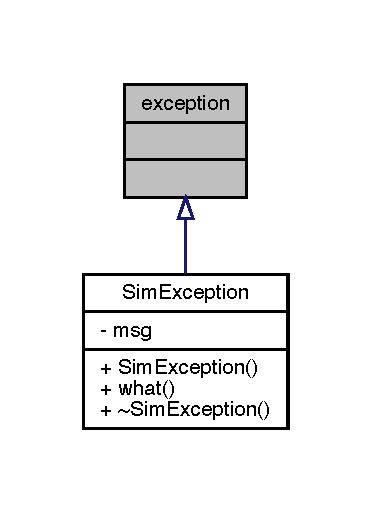
\includegraphics[width=178pt]{classexception__inherit__graph}
\end{center}
\end{figure}


Collaboration diagram for exception\+:\nopagebreak
\begin{figure}[H]
\begin{center}
\leavevmode
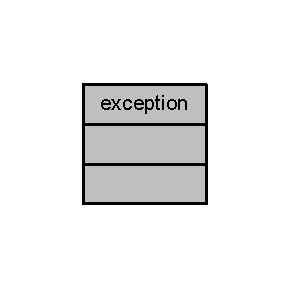
\includegraphics[width=139pt]{classexception__coll__graph}
\end{center}
\end{figure}


The documentation for this class was generated from the following file\+:\begin{DoxyCompactItemize}
\item 
include/\hyperlink{_sim_exception_8h}{Sim\+Exception.\+h}\end{DoxyCompactItemize}

\hypertarget{class_grid}{}\section{Grid Class Reference}
\label{class_grid}\index{Grid@{Grid}}


{\ttfamily \#include $<$Grid.\+h$>$}



Collaboration diagram for Grid\+:
\nopagebreak
\begin{figure}[H]
\begin{center}
\leavevmode
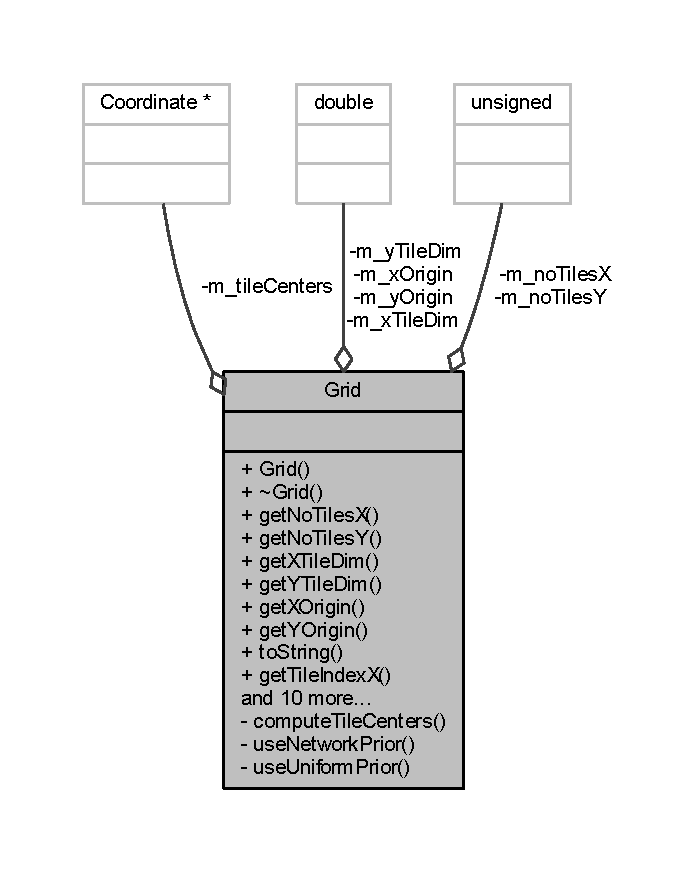
\includegraphics[width=332pt]{class_grid__coll__graph}
\end{center}
\end{figure}
\subsection*{Public Member Functions}
\begin{DoxyCompactItemize}
\item 
\hyperlink{class_grid_a84b0dc169028f21175a4549afde86153}{Grid} (double x\+Orig, double y\+Orig, double x\+Tiledim, double y\+Tiledim, unsigned long no\+TilesX, unsigned long no\+TilesY)
\item 
virtual \hyperlink{class_grid_a241c623291936ddbf4f670a796523a91}{$\sim$\+Grid} ()
\item 
unsigned long \hyperlink{class_grid_af29c0c404a908aa46f83afb17d7609a6}{get\+No\+TilesX} () const
\item 
unsigned long \hyperlink{class_grid_a783a3153d03154cfd33e6a418bb8d390}{get\+No\+TilesY} () const
\item 
double \hyperlink{class_grid_a1c5b9ad91fac264bcdd67f99bc93f663}{get\+X\+Tile\+Dim} () const
\item 
double \hyperlink{class_grid_aedfe477f5be79a375bd64a4d21765918}{get\+Y\+Tile\+Dim} () const
\item 
double \hyperlink{class_grid_a08b534c7f8e1099a6903bf08d9727842}{get\+X\+Origin} () const
\item 
double \hyperlink{class_grid_a53141770920cf261579cf164a8909af9}{get\+Y\+Origin} () const
\item 
const unsigned long \hyperlink{class_grid_ab0a71c762b6c33e6fa2fd49dde38228b}{get\+No\+Tiles} () const
\item 
Coordinate \hyperlink{class_grid_aa8d3de015a2b22d0cd0d72b3e7c29088}{get\+Tile\+Center} (unsigned long tile\+Index) const
\item 
unsigned long \hyperlink{class_grid_a93e42713b7af1f188ce90f92a5e202ab}{get\+Tile\+No} (const Point $\ast$p) const
\item 
unsigned long \hyperlink{class_grid_a02dee9ad3ee575623916c0041f72eb5e}{get\+Tile\+No} (double x, double y) const
\item 
void \hyperlink{class_grid_a0024d8d3cdd7b95f9fd61205ce8b9dea}{dump\+Grid} (const string \&grid\+File\+Name) const
\item 
Coordinate $\ast$ \hyperlink{class_grid_aa1b1f4c938207b16694a27cb9beb66eb}{get\+Tile\+Centers} () const
\end{DoxyCompactItemize}
\subsection*{Private Member Functions}
\begin{DoxyCompactItemize}
\item 
unsigned long \hyperlink{class_grid_a5ab67c336ac08c690a0e8b03c12f02e5}{get\+Tile\+IndexX} (double x) const
\item 
unsigned long \hyperlink{class_grid_ad745f856bb2b27382118ac03fafc06b4}{get\+Tile\+IndexY} (double y) const
\item 
unsigned long \hyperlink{class_grid_af4094832e2adedbbd47889973f5a40da}{get\+Tile\+IndexX} (const Point $\ast$p) const
\item 
unsigned long \hyperlink{class_grid_ae1eeb3b42007ae1cf19cfaf0d846fb9a}{get\+Tile\+IndexY} (const Point $\ast$p) const
\item 
string \hyperlink{class_grid_ad48d195b5e333a94a3a14d6395252b2a}{to\+String} () const
\item 
Coordinate $\ast$ \hyperlink{class_grid_a8948d61db8ba1bda2260590677eaaa01}{compute\+Tile\+Centers} ()
\end{DoxyCompactItemize}
\subsection*{Private Attributes}
\begin{DoxyCompactItemize}
\item 
double \hyperlink{class_grid_ae109d428ac5489815748e92fdde1b91f}{m\+\_\+x\+Origin}
\item 
double \hyperlink{class_grid_a16b2fc5a6e96ad2d59d59b52db83f4aa}{m\+\_\+y\+Origin}
\item 
double \hyperlink{class_grid_a48c3d1fc34a14bff8b9176558a8b6f4e}{m\+\_\+x\+Tile\+Dim}
\item 
double \hyperlink{class_grid_a497eeffc4a16a021e15ecbc130f4f644}{m\+\_\+y\+Tile\+Dim}
\item 
unsigned long \hyperlink{class_grid_a177bfdc70436c25a1510d1abe19e34c1}{m\+\_\+no\+TilesX}
\item 
unsigned long \hyperlink{class_grid_a8fe14c4781dfd5623922fcc1f9c10130}{m\+\_\+no\+TilesY}
\item 
Coordinate $\ast$ \hyperlink{class_grid_a27b99b13ac7e5bec81f7b8704bc3405a}{m\+\_\+tile\+Centers}
\end{DoxyCompactItemize}


\subsection{Detailed Description}
This class implements a grid of rectangular tiles overlapped on the map of the simulation. This grid is used to compute the \char`\"{}observed\char`\"{} location of a mobile phone. This means that we compute the probability of a mobile device to be in a specific tile of the grid using the data recorded by each antenna during the simulation. A finer grid will give a more accurate location but the computational cost increase when the size of the tiles decrease. The tiles of the grid are indexed starting with 0 for the tile in the bottom left corner of the grid in a row-\/major ordering. The last tile, with the biggest index, is the tile in the upper-\/right corner of the grid. 

\subsection{Constructor \& Destructor Documentation}
\mbox{\Hypertarget{class_grid_a84b0dc169028f21175a4549afde86153}\label{class_grid_a84b0dc169028f21175a4549afde86153}} 
\index{Grid@{Grid}!Grid@{Grid}}
\index{Grid@{Grid}!Grid@{Grid}}
\subsubsection{\texorpdfstring{Grid()}{Grid()}}
{\footnotesize\ttfamily Grid\+::\+Grid (\begin{DoxyParamCaption}\item[{double}]{x\+Orig,  }\item[{double}]{y\+Orig,  }\item[{double}]{x\+Tiledim,  }\item[{double}]{y\+Tiledim,  }\item[{unsigned long}]{no\+TilesX,  }\item[{unsigned long}]{no\+TilesY }\end{DoxyParamCaption})}

Constructor of the class. Build a \hyperlink{class_grid}{Grid} object with the specified parameters. 
\begin{DoxyParams}{Parameters}
{\em x\+Orig} & the x coordinate of the origin of the grid (i.\+e. the x coordinate of the bottom left corner of the grid). \\
\hline
{\em y\+Orig} & the y coordinate of the origin of the grid (i.\+e. the y coordinate of the bottom left corner of the grid). \\
\hline
{\em x\+Tiledim} & the dimension of a tile on X axis. \\
\hline
{\em y\+Tiledim} & the dimension of a tile on Y axis. \\
\hline
{\em no\+TilesX} & the number of tiles on X axis. \\
\hline
{\em no\+TilesY} & the number of tiles on Y axis. \\
\hline
\end{DoxyParams}
\mbox{\Hypertarget{class_grid_a241c623291936ddbf4f670a796523a91}\label{class_grid_a241c623291936ddbf4f670a796523a91}} 
\index{Grid@{Grid}!````~Grid@{$\sim$\+Grid}}
\index{````~Grid@{$\sim$\+Grid}!Grid@{Grid}}
\subsubsection{\texorpdfstring{$\sim$\+Grid()}{~Grid()}}
{\footnotesize\ttfamily virtual Grid\+::$\sim$\+Grid (\begin{DoxyParamCaption}{ }\end{DoxyParamCaption})\hspace{0.3cm}{\ttfamily [virtual]}}

Default destructor. 

\subsection{Member Function Documentation}
\mbox{\Hypertarget{class_grid_a8948d61db8ba1bda2260590677eaaa01}\label{class_grid_a8948d61db8ba1bda2260590677eaaa01}} 
\index{Grid@{Grid}!compute\+Tile\+Centers@{compute\+Tile\+Centers}}
\index{compute\+Tile\+Centers@{compute\+Tile\+Centers}!Grid@{Grid}}
\subsubsection{\texorpdfstring{compute\+Tile\+Centers()}{computeTileCenters()}}
{\footnotesize\ttfamily Coordinate$\ast$ Grid\+::compute\+Tile\+Centers (\begin{DoxyParamCaption}{ }\end{DoxyParamCaption})\hspace{0.3cm}{\ttfamily [private]}}

\mbox{\Hypertarget{class_grid_a0024d8d3cdd7b95f9fd61205ce8b9dea}\label{class_grid_a0024d8d3cdd7b95f9fd61205ce8b9dea}} 
\index{Grid@{Grid}!dump\+Grid@{dump\+Grid}}
\index{dump\+Grid@{dump\+Grid}!Grid@{Grid}}
\subsubsection{\texorpdfstring{dump\+Grid()}{dumpGrid()}}
{\footnotesize\ttfamily void Grid\+::dump\+Grid (\begin{DoxyParamCaption}\item[{const string \&}]{grid\+File\+Name }\end{DoxyParamCaption}) const}

Writes the grid description in a .csv file for later processing. 
\begin{DoxyParams}{Parameters}
{\em grid\+File\+Name} & the name of the output file. \\
\hline
\end{DoxyParams}
\mbox{\Hypertarget{class_grid_ab0a71c762b6c33e6fa2fd49dde38228b}\label{class_grid_ab0a71c762b6c33e6fa2fd49dde38228b}} 
\index{Grid@{Grid}!get\+No\+Tiles@{get\+No\+Tiles}}
\index{get\+No\+Tiles@{get\+No\+Tiles}!Grid@{Grid}}
\subsubsection{\texorpdfstring{get\+No\+Tiles()}{getNoTiles()}}
{\footnotesize\ttfamily const unsigned long Grid\+::get\+No\+Tiles (\begin{DoxyParamCaption}{ }\end{DoxyParamCaption}) const}

Computes the total number of tiles in the grid. \begin{DoxyReturn}{Returns}
the total number of tiles in the grid. 
\end{DoxyReturn}
\mbox{\Hypertarget{class_grid_af29c0c404a908aa46f83afb17d7609a6}\label{class_grid_af29c0c404a908aa46f83afb17d7609a6}} 
\index{Grid@{Grid}!get\+No\+TilesX@{get\+No\+TilesX}}
\index{get\+No\+TilesX@{get\+No\+TilesX}!Grid@{Grid}}
\subsubsection{\texorpdfstring{get\+No\+Tiles\+X()}{getNoTilesX()}}
{\footnotesize\ttfamily unsigned long Grid\+::get\+No\+TilesX (\begin{DoxyParamCaption}{ }\end{DoxyParamCaption}) const}

\begin{DoxyReturn}{Returns}
the number of tiles of the grid on X axis direction. 
\end{DoxyReturn}
\mbox{\Hypertarget{class_grid_a783a3153d03154cfd33e6a418bb8d390}\label{class_grid_a783a3153d03154cfd33e6a418bb8d390}} 
\index{Grid@{Grid}!get\+No\+TilesY@{get\+No\+TilesY}}
\index{get\+No\+TilesY@{get\+No\+TilesY}!Grid@{Grid}}
\subsubsection{\texorpdfstring{get\+No\+Tiles\+Y()}{getNoTilesY()}}
{\footnotesize\ttfamily unsigned long Grid\+::get\+No\+TilesY (\begin{DoxyParamCaption}{ }\end{DoxyParamCaption}) const}

\begin{DoxyReturn}{Returns}
the number of tiles of the grid on Y axis direction. 
\end{DoxyReturn}
\mbox{\Hypertarget{class_grid_aa8d3de015a2b22d0cd0d72b3e7c29088}\label{class_grid_aa8d3de015a2b22d0cd0d72b3e7c29088}} 
\index{Grid@{Grid}!get\+Tile\+Center@{get\+Tile\+Center}}
\index{get\+Tile\+Center@{get\+Tile\+Center}!Grid@{Grid}}
\subsubsection{\texorpdfstring{get\+Tile\+Center()}{getTileCenter()}}
{\footnotesize\ttfamily Coordinate Grid\+::get\+Tile\+Center (\begin{DoxyParamCaption}\item[{unsigned long}]{tile\+Index }\end{DoxyParamCaption}) const}

Computes the coordinates of the tile center given by its index in the grid. 
\begin{DoxyParams}{Parameters}
{\em tile\+Index} & the tile index. \\
\hline
\end{DoxyParams}
\begin{DoxyReturn}{Returns}
the coordinates of the center of the tile. 
\end{DoxyReturn}
\mbox{\Hypertarget{class_grid_aa1b1f4c938207b16694a27cb9beb66eb}\label{class_grid_aa1b1f4c938207b16694a27cb9beb66eb}} 
\index{Grid@{Grid}!get\+Tile\+Centers@{get\+Tile\+Centers}}
\index{get\+Tile\+Centers@{get\+Tile\+Centers}!Grid@{Grid}}
\subsubsection{\texorpdfstring{get\+Tile\+Centers()}{getTileCenters()}}
{\footnotesize\ttfamily Coordinate$\ast$ Grid\+::get\+Tile\+Centers (\begin{DoxyParamCaption}{ }\end{DoxyParamCaption}) const}

Returns a vector containing the coordinates of the tile centers. \begin{DoxyReturn}{Returns}
a vector containing the coordinates of the tile centers. 
\end{DoxyReturn}
\mbox{\Hypertarget{class_grid_a5ab67c336ac08c690a0e8b03c12f02e5}\label{class_grid_a5ab67c336ac08c690a0e8b03c12f02e5}} 
\index{Grid@{Grid}!get\+Tile\+IndexX@{get\+Tile\+IndexX}}
\index{get\+Tile\+IndexX@{get\+Tile\+IndexX}!Grid@{Grid}}
\subsubsection{\texorpdfstring{get\+Tile\+Index\+X()}{getTileIndexX()}\hspace{0.1cm}{\footnotesize\ttfamily [1/2]}}
{\footnotesize\ttfamily unsigned long Grid\+::get\+Tile\+IndexX (\begin{DoxyParamCaption}\item[{double}]{x }\end{DoxyParamCaption}) const\hspace{0.3cm}{\ttfamily [private]}}

\mbox{\Hypertarget{class_grid_af4094832e2adedbbd47889973f5a40da}\label{class_grid_af4094832e2adedbbd47889973f5a40da}} 
\index{Grid@{Grid}!get\+Tile\+IndexX@{get\+Tile\+IndexX}}
\index{get\+Tile\+IndexX@{get\+Tile\+IndexX}!Grid@{Grid}}
\subsubsection{\texorpdfstring{get\+Tile\+Index\+X()}{getTileIndexX()}\hspace{0.1cm}{\footnotesize\ttfamily [2/2]}}
{\footnotesize\ttfamily unsigned long Grid\+::get\+Tile\+IndexX (\begin{DoxyParamCaption}\item[{const Point $\ast$}]{p }\end{DoxyParamCaption}) const\hspace{0.3cm}{\ttfamily [private]}}

Returns the tile index on X axis that contains a given point in space, specified by p. 
\begin{DoxyParams}{Parameters}
{\em p} & a pointer to the point for which we need the tile index. \\
\hline
\end{DoxyParams}
\begin{DoxyReturn}{Returns}
the tile index on X axis that contains the point specified by p, i.\+e. a number between 0 and \hyperlink{class_grid_af29c0c404a908aa46f83afb17d7609a6}{get\+No\+Tiles\+X()} -\/ 1. 
\end{DoxyReturn}
\mbox{\Hypertarget{class_grid_ad745f856bb2b27382118ac03fafc06b4}\label{class_grid_ad745f856bb2b27382118ac03fafc06b4}} 
\index{Grid@{Grid}!get\+Tile\+IndexY@{get\+Tile\+IndexY}}
\index{get\+Tile\+IndexY@{get\+Tile\+IndexY}!Grid@{Grid}}
\subsubsection{\texorpdfstring{get\+Tile\+Index\+Y()}{getTileIndexY()}\hspace{0.1cm}{\footnotesize\ttfamily [1/2]}}
{\footnotesize\ttfamily unsigned long Grid\+::get\+Tile\+IndexY (\begin{DoxyParamCaption}\item[{double}]{y }\end{DoxyParamCaption}) const\hspace{0.3cm}{\ttfamily [private]}}

\mbox{\Hypertarget{class_grid_ae1eeb3b42007ae1cf19cfaf0d846fb9a}\label{class_grid_ae1eeb3b42007ae1cf19cfaf0d846fb9a}} 
\index{Grid@{Grid}!get\+Tile\+IndexY@{get\+Tile\+IndexY}}
\index{get\+Tile\+IndexY@{get\+Tile\+IndexY}!Grid@{Grid}}
\subsubsection{\texorpdfstring{get\+Tile\+Index\+Y()}{getTileIndexY()}\hspace{0.1cm}{\footnotesize\ttfamily [2/2]}}
{\footnotesize\ttfamily unsigned long Grid\+::get\+Tile\+IndexY (\begin{DoxyParamCaption}\item[{const Point $\ast$}]{p }\end{DoxyParamCaption}) const\hspace{0.3cm}{\ttfamily [private]}}

Returns the tile index on Y axis that contains a given point in space, specified by p. 
\begin{DoxyParams}{Parameters}
{\em p} & the point in space for which we need the tile index. \\
\hline
\end{DoxyParams}
\begin{DoxyReturn}{Returns}
the tile index on Y axis that contains the point specified by p, i.\+e. a number between 0 and \hyperlink{class_grid_a783a3153d03154cfd33e6a418bb8d390}{get\+No\+Tiles\+Y()} -\/ 1. 
\end{DoxyReturn}
\mbox{\Hypertarget{class_grid_a93e42713b7af1f188ce90f92a5e202ab}\label{class_grid_a93e42713b7af1f188ce90f92a5e202ab}} 
\index{Grid@{Grid}!get\+Tile\+No@{get\+Tile\+No}}
\index{get\+Tile\+No@{get\+Tile\+No}!Grid@{Grid}}
\subsubsection{\texorpdfstring{get\+Tile\+No()}{getTileNo()}\hspace{0.1cm}{\footnotesize\ttfamily [1/2]}}
{\footnotesize\ttfamily unsigned long Grid\+::get\+Tile\+No (\begin{DoxyParamCaption}\item[{const Point $\ast$}]{p }\end{DoxyParamCaption}) const}

Computes the tile index of the tile that contains the Point indicated by p. 
\begin{DoxyParams}{Parameters}
{\em p} & a pointer to a Point object. \\
\hline
\end{DoxyParams}
\begin{DoxyReturn}{Returns}
the tile index of the tile that contains the Point indicated by p. 
\end{DoxyReturn}
\mbox{\Hypertarget{class_grid_a02dee9ad3ee575623916c0041f72eb5e}\label{class_grid_a02dee9ad3ee575623916c0041f72eb5e}} 
\index{Grid@{Grid}!get\+Tile\+No@{get\+Tile\+No}}
\index{get\+Tile\+No@{get\+Tile\+No}!Grid@{Grid}}
\subsubsection{\texorpdfstring{get\+Tile\+No()}{getTileNo()}\hspace{0.1cm}{\footnotesize\ttfamily [2/2]}}
{\footnotesize\ttfamily unsigned long Grid\+::get\+Tile\+No (\begin{DoxyParamCaption}\item[{double}]{x,  }\item[{double}]{y }\end{DoxyParamCaption}) const}

Computes the tile index of the tile that contains a point with coordinates indicated by x and y. 
\begin{DoxyParams}{Parameters}
{\em x} & x coordinate of a location. \\
\hline
{\em y} & y coordinate of a location. \\
\hline
\end{DoxyParams}
\begin{DoxyReturn}{Returns}
the tile index of the tile that contains a point with coordinates indicated by x and y. 
\end{DoxyReturn}
\mbox{\Hypertarget{class_grid_a08b534c7f8e1099a6903bf08d9727842}\label{class_grid_a08b534c7f8e1099a6903bf08d9727842}} 
\index{Grid@{Grid}!get\+X\+Origin@{get\+X\+Origin}}
\index{get\+X\+Origin@{get\+X\+Origin}!Grid@{Grid}}
\subsubsection{\texorpdfstring{get\+X\+Origin()}{getXOrigin()}}
{\footnotesize\ttfamily double Grid\+::get\+X\+Origin (\begin{DoxyParamCaption}{ }\end{DoxyParamCaption}) const}

\begin{DoxyReturn}{Returns}
the x coordinate of the origin of the grid (i.\+e. the x coordinate of the bottom left corner of the grid). 
\end{DoxyReturn}
\mbox{\Hypertarget{class_grid_a1c5b9ad91fac264bcdd67f99bc93f663}\label{class_grid_a1c5b9ad91fac264bcdd67f99bc93f663}} 
\index{Grid@{Grid}!get\+X\+Tile\+Dim@{get\+X\+Tile\+Dim}}
\index{get\+X\+Tile\+Dim@{get\+X\+Tile\+Dim}!Grid@{Grid}}
\subsubsection{\texorpdfstring{get\+X\+Tile\+Dim()}{getXTileDim()}}
{\footnotesize\ttfamily double Grid\+::get\+X\+Tile\+Dim (\begin{DoxyParamCaption}{ }\end{DoxyParamCaption}) const}

\begin{DoxyReturn}{Returns}
the dimension of a tile on X axis direction. 
\end{DoxyReturn}
\mbox{\Hypertarget{class_grid_a53141770920cf261579cf164a8909af9}\label{class_grid_a53141770920cf261579cf164a8909af9}} 
\index{Grid@{Grid}!get\+Y\+Origin@{get\+Y\+Origin}}
\index{get\+Y\+Origin@{get\+Y\+Origin}!Grid@{Grid}}
\subsubsection{\texorpdfstring{get\+Y\+Origin()}{getYOrigin()}}
{\footnotesize\ttfamily double Grid\+::get\+Y\+Origin (\begin{DoxyParamCaption}{ }\end{DoxyParamCaption}) const}

\begin{DoxyReturn}{Returns}
the y coordinate of the origin of the grid (i.\+e. the y coordinate of the bottom left corner of the grid). 
\end{DoxyReturn}
\mbox{\Hypertarget{class_grid_aedfe477f5be79a375bd64a4d21765918}\label{class_grid_aedfe477f5be79a375bd64a4d21765918}} 
\index{Grid@{Grid}!get\+Y\+Tile\+Dim@{get\+Y\+Tile\+Dim}}
\index{get\+Y\+Tile\+Dim@{get\+Y\+Tile\+Dim}!Grid@{Grid}}
\subsubsection{\texorpdfstring{get\+Y\+Tile\+Dim()}{getYTileDim()}}
{\footnotesize\ttfamily double Grid\+::get\+Y\+Tile\+Dim (\begin{DoxyParamCaption}{ }\end{DoxyParamCaption}) const}

\begin{DoxyReturn}{Returns}
the dimension of a tile on Y axis direction. 
\end{DoxyReturn}
\mbox{\Hypertarget{class_grid_ad48d195b5e333a94a3a14d6395252b2a}\label{class_grid_ad48d195b5e333a94a3a14d6395252b2a}} 
\index{Grid@{Grid}!to\+String@{to\+String}}
\index{to\+String@{to\+String}!Grid@{Grid}}
\subsubsection{\texorpdfstring{to\+String()}{toString()}}
{\footnotesize\ttfamily string Grid\+::to\+String (\begin{DoxyParamCaption}{ }\end{DoxyParamCaption}) const\hspace{0.3cm}{\ttfamily [private]}}

\begin{DoxyReturn}{Returns}
a string representation of an object of type \hyperlink{class_grid}{Grid}. This is useful to write a textual description of the grid in a file for later processing. 
\end{DoxyReturn}


\subsection{Member Data Documentation}
\mbox{\Hypertarget{class_grid_a177bfdc70436c25a1510d1abe19e34c1}\label{class_grid_a177bfdc70436c25a1510d1abe19e34c1}} 
\index{Grid@{Grid}!m\+\_\+no\+TilesX@{m\+\_\+no\+TilesX}}
\index{m\+\_\+no\+TilesX@{m\+\_\+no\+TilesX}!Grid@{Grid}}
\subsubsection{\texorpdfstring{m\+\_\+no\+TilesX}{m\_noTilesX}}
{\footnotesize\ttfamily unsigned long Grid\+::m\+\_\+no\+TilesX\hspace{0.3cm}{\ttfamily [private]}}

\mbox{\Hypertarget{class_grid_a8fe14c4781dfd5623922fcc1f9c10130}\label{class_grid_a8fe14c4781dfd5623922fcc1f9c10130}} 
\index{Grid@{Grid}!m\+\_\+no\+TilesY@{m\+\_\+no\+TilesY}}
\index{m\+\_\+no\+TilesY@{m\+\_\+no\+TilesY}!Grid@{Grid}}
\subsubsection{\texorpdfstring{m\+\_\+no\+TilesY}{m\_noTilesY}}
{\footnotesize\ttfamily unsigned long Grid\+::m\+\_\+no\+TilesY\hspace{0.3cm}{\ttfamily [private]}}

\mbox{\Hypertarget{class_grid_a27b99b13ac7e5bec81f7b8704bc3405a}\label{class_grid_a27b99b13ac7e5bec81f7b8704bc3405a}} 
\index{Grid@{Grid}!m\+\_\+tile\+Centers@{m\+\_\+tile\+Centers}}
\index{m\+\_\+tile\+Centers@{m\+\_\+tile\+Centers}!Grid@{Grid}}
\subsubsection{\texorpdfstring{m\+\_\+tile\+Centers}{m\_tileCenters}}
{\footnotesize\ttfamily Coordinate$\ast$ Grid\+::m\+\_\+tile\+Centers\hspace{0.3cm}{\ttfamily [private]}}

\mbox{\Hypertarget{class_grid_ae109d428ac5489815748e92fdde1b91f}\label{class_grid_ae109d428ac5489815748e92fdde1b91f}} 
\index{Grid@{Grid}!m\+\_\+x\+Origin@{m\+\_\+x\+Origin}}
\index{m\+\_\+x\+Origin@{m\+\_\+x\+Origin}!Grid@{Grid}}
\subsubsection{\texorpdfstring{m\+\_\+x\+Origin}{m\_xOrigin}}
{\footnotesize\ttfamily double Grid\+::m\+\_\+x\+Origin\hspace{0.3cm}{\ttfamily [private]}}

\mbox{\Hypertarget{class_grid_a48c3d1fc34a14bff8b9176558a8b6f4e}\label{class_grid_a48c3d1fc34a14bff8b9176558a8b6f4e}} 
\index{Grid@{Grid}!m\+\_\+x\+Tile\+Dim@{m\+\_\+x\+Tile\+Dim}}
\index{m\+\_\+x\+Tile\+Dim@{m\+\_\+x\+Tile\+Dim}!Grid@{Grid}}
\subsubsection{\texorpdfstring{m\+\_\+x\+Tile\+Dim}{m\_xTileDim}}
{\footnotesize\ttfamily double Grid\+::m\+\_\+x\+Tile\+Dim\hspace{0.3cm}{\ttfamily [private]}}

\mbox{\Hypertarget{class_grid_a16b2fc5a6e96ad2d59d59b52db83f4aa}\label{class_grid_a16b2fc5a6e96ad2d59d59b52db83f4aa}} 
\index{Grid@{Grid}!m\+\_\+y\+Origin@{m\+\_\+y\+Origin}}
\index{m\+\_\+y\+Origin@{m\+\_\+y\+Origin}!Grid@{Grid}}
\subsubsection{\texorpdfstring{m\+\_\+y\+Origin}{m\_yOrigin}}
{\footnotesize\ttfamily double Grid\+::m\+\_\+y\+Origin\hspace{0.3cm}{\ttfamily [private]}}

\mbox{\Hypertarget{class_grid_a497eeffc4a16a021e15ecbc130f4f644}\label{class_grid_a497eeffc4a16a021e15ecbc130f4f644}} 
\index{Grid@{Grid}!m\+\_\+y\+Tile\+Dim@{m\+\_\+y\+Tile\+Dim}}
\index{m\+\_\+y\+Tile\+Dim@{m\+\_\+y\+Tile\+Dim}!Grid@{Grid}}
\subsubsection{\texorpdfstring{m\+\_\+y\+Tile\+Dim}{m\_yTileDim}}
{\footnotesize\ttfamily double Grid\+::m\+\_\+y\+Tile\+Dim\hspace{0.3cm}{\ttfamily [private]}}



The documentation for this class was generated from the following file\+:\begin{DoxyCompactItemize}
\item 
include/map/\hyperlink{_grid_8h}{Grid.\+h}\end{DoxyCompactItemize}

\section{Holdable\+Agent Class Reference}
\label{class_holdable_agent}\index{HoldableAgent@{HoldableAgent}}


{\ttfamily \#include $<$Holdable\+Agent.\+h$>$}

Inheritance diagram for Holdable\+Agent\+:\begin{figure}[H]
\begin{center}
\leavevmode
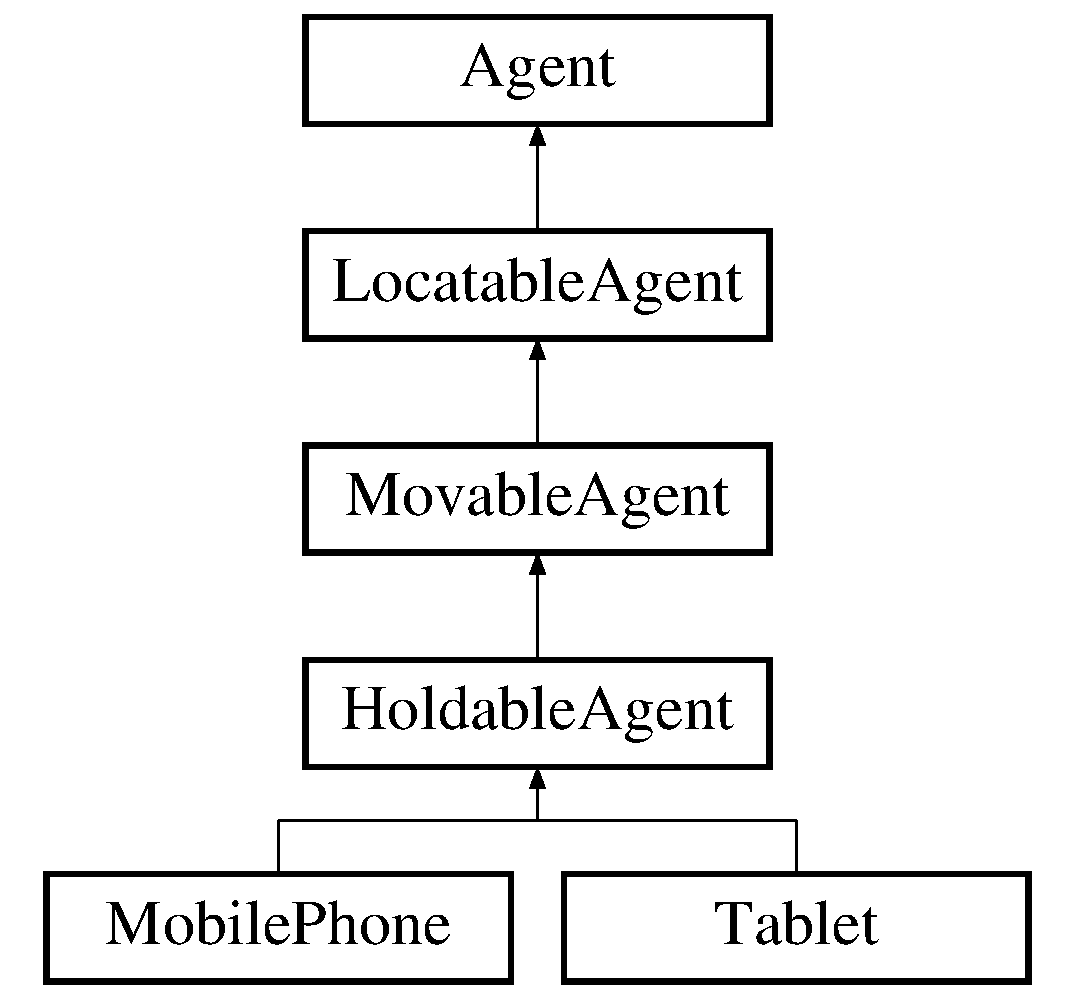
\includegraphics[height=5.000000cm]{class_holdable_agent}
\end{center}
\end{figure}
\subsection*{Public Types}
\begin{DoxyCompactItemize}
\item 
enum \textbf{ C\+O\+N\+N\+E\+C\+T\+I\+O\+N\+\_\+\+T\+Y\+PE} \{ \textbf{ U\+S\+I\+N\+G\+\_\+\+P\+O\+W\+ER}, 
\textbf{ U\+S\+I\+N\+G\+\_\+\+S\+I\+G\+N\+A\+L\+\_\+\+Q\+U\+A\+L\+I\+TY}, 
\textbf{ U\+N\+K\+N\+O\+WN}
 \}
\end{DoxyCompactItemize}
\subsection*{Public Member Functions}
\begin{DoxyCompactItemize}
\item 
\textbf{ Holdable\+Agent} (\textbf{ Map} $\ast$m, long id, Point $\ast$init\+Position, \textbf{ Agent} $\ast$holder, \textbf{ Clock} $\ast$clock)
\item 
\textbf{ Holdable\+Agent} (const \textbf{ Holdable\+Agent} \&h)
\item 
virtual \textbf{ $\sim$\+Holdable\+Agent} ()
\item 
\textbf{ Agent} $\ast$ \textbf{ get\+Holder} () const
\item 
void \textbf{ set\+Holder} (\textbf{ Agent} $\ast$holder)
\item 
string \textbf{ get\+Name} () override
\item 
string \textbf{ to\+String} () override
\item 
virtual bool \textbf{ try\+Connect} (\textbf{ C\+O\+N\+N\+E\+C\+T\+I\+O\+N\+\_\+\+T\+Y\+PE} type)=0
\item 
virtual bool \textbf{ is\+Connected} () const
\item 
void \textbf{ set\+Location} (Point $\ast$location) override
\item 
vector$<$ \textbf{ Antenna} $\ast$ $>$ \textbf{ get\+Antennas} () const
\end{DoxyCompactItemize}
\subsection*{Private Attributes}
\begin{DoxyCompactItemize}
\item 
\textbf{ Agent} $\ast$ \textbf{ m\+\_\+holder}
\item 
vector$<$ \textbf{ Antenna} $\ast$ $>$ \textbf{ m\+\_\+antennas}
\end{DoxyCompactItemize}


\subsection{Detailed Description}


Definition at line 21 of file Holdable\+Agent.\+h.



\subsection{Member Enumeration Documentation}
\mbox{\label{class_holdable_agent_ae2c334b004d7b9c5a999cf2618e4e518}} 
\index{HoldableAgent@{HoldableAgent}!CONNECTION\_TYPE@{CONNECTION\_TYPE}}
\index{CONNECTION\_TYPE@{CONNECTION\_TYPE}!HoldableAgent@{HoldableAgent}}
\subsubsection{CONNECTION\_TYPE}
{\footnotesize\ttfamily enum \textbf{ Holdable\+Agent\+::\+C\+O\+N\+N\+E\+C\+T\+I\+O\+N\+\_\+\+T\+Y\+PE}}

\begin{DoxyEnumFields}{Enumerator}
\raisebox{\heightof{T}}[0pt][0pt]{\index{USING\_POWER@{USING\_POWER}!HoldableAgent@{HoldableAgent}}\index{HoldableAgent@{HoldableAgent}!USING\_POWER@{USING\_POWER}}}\mbox{\label{class_holdable_agent_ae2c334b004d7b9c5a999cf2618e4e518ab8f4a3956d88a54e0aad08e89e203fd6}} 
U\+S\+I\+N\+G\+\_\+\+P\+O\+W\+ER&\\
\hline

\raisebox{\heightof{T}}[0pt][0pt]{\index{USING\_SIGNAL\_QUALITY@{USING\_SIGNAL\_QUALITY}!HoldableAgent@{HoldableAgent}}\index{HoldableAgent@{HoldableAgent}!USING\_SIGNAL\_QUALITY@{USING\_SIGNAL\_QUALITY}}}\mbox{\label{class_holdable_agent_ae2c334b004d7b9c5a999cf2618e4e518a93c5b260edf949c65b96fec443c33f2b}} 
U\+S\+I\+N\+G\+\_\+\+S\+I\+G\+N\+A\+L\+\_\+\+Q\+U\+A\+L\+I\+TY&\\
\hline

\raisebox{\heightof{T}}[0pt][0pt]{\index{UNKNOWN@{UNKNOWN}!HoldableAgent@{HoldableAgent}}\index{HoldableAgent@{HoldableAgent}!UNKNOWN@{UNKNOWN}}}\mbox{\label{class_holdable_agent_ae2c334b004d7b9c5a999cf2618e4e518a6bdb1529a2032a4648226328e179f552}} 
U\+N\+K\+N\+O\+WN&\\
\hline

\end{DoxyEnumFields}


Definition at line 25 of file Holdable\+Agent.\+h.



\subsection{Constructor \& Destructor Documentation}
\mbox{\label{class_holdable_agent_ab5060ddcd08291c60b49fec22d6bd6f3}} 
\index{HoldableAgent@{HoldableAgent}!HoldableAgent@{HoldableAgent}}
\index{HoldableAgent@{HoldableAgent}!HoldableAgent@{HoldableAgent}}
\subsubsection{HoldableAgent()\hspace{0.1cm}{\footnotesize\ttfamily [1/2]}}
{\footnotesize\ttfamily Holdable\+Agent\+::\+Holdable\+Agent (\begin{DoxyParamCaption}\item[{\textbf{ Map} $\ast$}]{m,  }\item[{long}]{id,  }\item[{Point $\ast$}]{init\+Position,  }\item[{\textbf{ Agent} $\ast$}]{holder,  }\item[{\textbf{ Clock} $\ast$}]{clock }\end{DoxyParamCaption})\hspace{0.3cm}{\ttfamily [explicit]}}



Definition at line 16 of file Holdable\+Agent.\+cpp.

\mbox{\label{class_holdable_agent_a9b7c1494266c0a807d809461b59ced80}} 
\index{HoldableAgent@{HoldableAgent}!HoldableAgent@{HoldableAgent}}
\index{HoldableAgent@{HoldableAgent}!HoldableAgent@{HoldableAgent}}
\subsubsection{HoldableAgent()\hspace{0.1cm}{\footnotesize\ttfamily [2/2]}}
{\footnotesize\ttfamily Holdable\+Agent\+::\+Holdable\+Agent (\begin{DoxyParamCaption}\item[{const \textbf{ Holdable\+Agent} \&}]{h }\end{DoxyParamCaption})}



Definition at line 22 of file Holdable\+Agent.\+cpp.



References get\+Antennas(), get\+Holder(), m\+\_\+antennas, and m\+\_\+holder.

\mbox{\label{class_holdable_agent_ab529d1f070a574375a79baadc89e9b78}} 
\index{HoldableAgent@{HoldableAgent}!````~HoldableAgent@{$\sim$HoldableAgent}}
\index{````~HoldableAgent@{$\sim$HoldableAgent}!HoldableAgent@{HoldableAgent}}
\subsubsection{$\sim$HoldableAgent()}
{\footnotesize\ttfamily Holdable\+Agent\+::$\sim$\+Holdable\+Agent (\begin{DoxyParamCaption}{ }\end{DoxyParamCaption})\hspace{0.3cm}{\ttfamily [virtual]}}



Definition at line 29 of file Holdable\+Agent.\+cpp.



\subsection{Member Function Documentation}
\mbox{\label{class_holdable_agent_af04b66d8148877c40e1fa0a5fef4b546}} 
\index{HoldableAgent@{HoldableAgent}!getAntennas@{getAntennas}}
\index{getAntennas@{getAntennas}!HoldableAgent@{HoldableAgent}}
\subsubsection{getAntennas()}
{\footnotesize\ttfamily vector$<$ \textbf{ Antenna} $\ast$ $>$ Holdable\+Agent\+::get\+Antennas (\begin{DoxyParamCaption}{ }\end{DoxyParamCaption}) const}



Definition at line 54 of file Holdable\+Agent.\+cpp.



References m\+\_\+antennas.



Referenced by Holdable\+Agent().

\mbox{\label{class_holdable_agent_a4fdf36fd8fb79a168360ebf74b9ba61d}} 
\index{HoldableAgent@{HoldableAgent}!getHolder@{getHolder}}
\index{getHolder@{getHolder}!HoldableAgent@{HoldableAgent}}
\subsubsection{getHolder()}
{\footnotesize\ttfamily \textbf{ Agent} $\ast$ Holdable\+Agent\+::get\+Holder (\begin{DoxyParamCaption}{ }\end{DoxyParamCaption}) const}



Definition at line 33 of file Holdable\+Agent.\+cpp.



References m\+\_\+holder.



Referenced by Holdable\+Agent().

\mbox{\label{class_holdable_agent_a089a15867a877d3a4cb510169c32d682}} 
\index{HoldableAgent@{HoldableAgent}!getName@{getName}}
\index{getName@{getName}!HoldableAgent@{HoldableAgent}}
\subsubsection{getName()}
{\footnotesize\ttfamily string Holdable\+Agent\+::get\+Name (\begin{DoxyParamCaption}{ }\end{DoxyParamCaption})\hspace{0.3cm}{\ttfamily [inline]}, {\ttfamily [override]}, {\ttfamily [virtual]}}



Implements \textbf{ Agent} \doxyref{}{p.}{class_agent_aa24682b2e0c8031d0637c156f6bee0e0}.



Reimplemented in \textbf{ Mobile\+Phone} \doxyref{}{p.}{class_mobile_phone_aa4f050bb755994fadfeab94c1f2147f7}, and \textbf{ Tablet} \doxyref{}{p.}{class_tablet_a2cac00cd9efca5b8adeff28ae5827970}.



Definition at line 34 of file Holdable\+Agent.\+h.

\mbox{\label{class_holdable_agent_a5d7b3db4bf6044736d80de1677afdeec}} 
\index{HoldableAgent@{HoldableAgent}!isConnected@{isConnected}}
\index{isConnected@{isConnected}!HoldableAgent@{HoldableAgent}}
\subsubsection{isConnected()}
{\footnotesize\ttfamily bool Holdable\+Agent\+::is\+Connected (\begin{DoxyParamCaption}{ }\end{DoxyParamCaption}) const\hspace{0.3cm}{\ttfamily [virtual]}}



Definition at line 50 of file Holdable\+Agent.\+cpp.



References m\+\_\+antennas.

\mbox{\label{class_holdable_agent_a39b53c9c6cacca716f38fccc520e9f52}} 
\index{HoldableAgent@{HoldableAgent}!setHolder@{setHolder}}
\index{setHolder@{setHolder}!HoldableAgent@{HoldableAgent}}
\subsubsection{setHolder()}
{\footnotesize\ttfamily void Holdable\+Agent\+::set\+Holder (\begin{DoxyParamCaption}\item[{\textbf{ Agent} $\ast$}]{holder }\end{DoxyParamCaption})}



Definition at line 37 of file Holdable\+Agent.\+cpp.



References Locatable\+Agent\+::get\+Location(), m\+\_\+holder, set\+Location(), and Movable\+Agent\+::set\+Speed().

\mbox{\label{class_holdable_agent_aec98d2fe325b48d9a84ad3dad44700e0}} 
\index{HoldableAgent@{HoldableAgent}!setLocation@{setLocation}}
\index{setLocation@{setLocation}!HoldableAgent@{HoldableAgent}}
\subsubsection{setLocation()}
{\footnotesize\ttfamily void Holdable\+Agent\+::set\+Location (\begin{DoxyParamCaption}\item[{Point $\ast$}]{location }\end{DoxyParamCaption})\hspace{0.3cm}{\ttfamily [override]}, {\ttfamily [virtual]}}



Reimplemented from \textbf{ Locatable\+Agent} \doxyref{}{p.}{class_locatable_agent_a4185a45957d529a7f57d19ea294cae81}.



Definition at line 58 of file Holdable\+Agent.\+cpp.



References Locatable\+Agent\+::set\+Location(), and try\+Connect().



Referenced by set\+Holder(), and Person\+::set\+Location().

\mbox{\label{class_holdable_agent_a3fee3021111198ac01469a715093ab88}} 
\index{HoldableAgent@{HoldableAgent}!toString@{toString}}
\index{toString@{toString}!HoldableAgent@{HoldableAgent}}
\subsubsection{toString()}
{\footnotesize\ttfamily string Holdable\+Agent\+::to\+String (\begin{DoxyParamCaption}{ }\end{DoxyParamCaption})\hspace{0.3cm}{\ttfamily [override]}, {\ttfamily [virtual]}}



Implements \textbf{ Agent} \doxyref{}{p.}{class_agent_a530b76f9163b2b8c19e7cdf8065888ac}.



Reimplemented in \textbf{ Mobile\+Phone} \doxyref{}{p.}{class_mobile_phone_a3e4bf0a37331042084ae703666f8fb7c}, and \textbf{ Tablet} \doxyref{}{p.}{class_tablet_a90880cd8f4a4afd451645e6e1dc86c5b}.



Definition at line 63 of file Holdable\+Agent.\+cpp.



References Agent\+::get\+Id(), m\+\_\+holder, and Movable\+Agent\+::to\+String().



Referenced by Tablet\+::to\+String(), and Mobile\+Phone\+::to\+String().

\mbox{\label{class_holdable_agent_a3f6500c10b054ca06a7800d4b01c5308}} 
\index{HoldableAgent@{HoldableAgent}!tryConnect@{tryConnect}}
\index{tryConnect@{tryConnect}!HoldableAgent@{HoldableAgent}}
\subsubsection{tryConnect()}
{\footnotesize\ttfamily virtual bool Holdable\+Agent\+::try\+Connect (\begin{DoxyParamCaption}\item[{\textbf{ C\+O\+N\+N\+E\+C\+T\+I\+O\+N\+\_\+\+T\+Y\+PE}}]{type }\end{DoxyParamCaption})\hspace{0.3cm}{\ttfamily [pure virtual]}}



Implemented in \textbf{ Mobile\+Phone} \doxyref{}{p.}{class_mobile_phone_a384f2a32e076dd34fdd1e814e1a48c11}, and \textbf{ Tablet} \doxyref{}{p.}{class_tablet_a4a08098f3acddd3167fc9633deabb809}.



Referenced by set\+Location().



\subsection{Member Data Documentation}
\mbox{\label{class_holdable_agent_a5f104212204e4c6761bed1d61fab100b}} 
\index{HoldableAgent@{HoldableAgent}!m\_antennas@{m\_antennas}}
\index{m\_antennas@{m\_antennas}!HoldableAgent@{HoldableAgent}}
\subsubsection{m\_antennas}
{\footnotesize\ttfamily vector$<$\textbf{ Antenna}$\ast$$>$ Holdable\+Agent\+::m\+\_\+antennas\hspace{0.3cm}{\ttfamily [private]}}



Definition at line 47 of file Holdable\+Agent.\+h.



Referenced by get\+Antennas(), Holdable\+Agent(), and is\+Connected().

\mbox{\label{class_holdable_agent_ae9c449c1831f933b5b6b6f71e425279b}} 
\index{HoldableAgent@{HoldableAgent}!m\_holder@{m\_holder}}
\index{m\_holder@{m\_holder}!HoldableAgent@{HoldableAgent}}
\subsubsection{m\_holder}
{\footnotesize\ttfamily \textbf{ Agent}$\ast$ Holdable\+Agent\+::m\+\_\+holder\hspace{0.3cm}{\ttfamily [private]}}



Definition at line 46 of file Holdable\+Agent.\+h.



Referenced by get\+Holder(), Holdable\+Agent(), set\+Holder(), and to\+String().



The documentation for this class was generated from the following files\+:\begin{DoxyCompactItemize}
\item 
include/\textbf{ Holdable\+Agent.\+h}\item 
src/\textbf{ Holdable\+Agent.\+cpp}\end{DoxyCompactItemize}

\hypertarget{class_i_d_generator}{}\section{I\+D\+Generator Class Reference}
\label{class_i_d_generator}\index{I\+D\+Generator@{I\+D\+Generator}}


{\ttfamily \#include $<$I\+D\+Generator.\+h$>$}



Collaboration diagram for I\+D\+Generator\+:\nopagebreak
\begin{figure}[H]
\begin{center}
\leavevmode
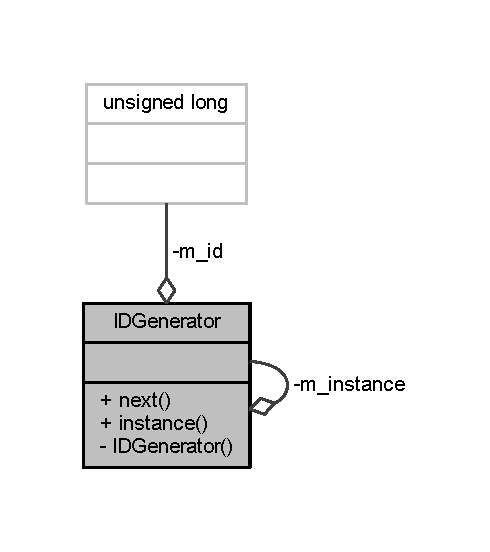
\includegraphics[width=235pt]{class_i_d_generator__coll__graph}
\end{center}
\end{figure}
\subsection*{Public Member Functions}
\begin{DoxyCompactItemize}
\item 
unsigned long \hyperlink{class_i_d_generator_a99d8cabb2ec6a17888a8ccbe9c85fee0}{next} ()
\end{DoxyCompactItemize}
\subsection*{Static Public Member Functions}
\begin{DoxyCompactItemize}
\item 
static \hyperlink{class_i_d_generator}{I\+D\+Generator} $\ast$ \hyperlink{class_i_d_generator_ad852c6dadc89e1020e4b3932f5a97bb3}{instance} ()
\end{DoxyCompactItemize}
\subsection*{Private Member Functions}
\begin{DoxyCompactItemize}
\item 
\hyperlink{class_i_d_generator_a8209b55f50b469c47f977660a769b1da}{I\+D\+Generator} ()
\end{DoxyCompactItemize}
\subsection*{Private Attributes}
\begin{DoxyCompactItemize}
\item 
unsigned long \hyperlink{class_i_d_generator_ad0400380525f694b23ff675f4f170893}{m\+\_\+id}
\end{DoxyCompactItemize}
\subsection*{Static Private Attributes}
\begin{DoxyCompactItemize}
\item 
static \hyperlink{class_i_d_generator}{I\+D\+Generator} $\ast$ \hyperlink{class_i_d_generator_a316bacdda67f4cf9bf73fcbd9bf94245}{m\+\_\+instance}
\end{DoxyCompactItemize}


\subsection{Detailed Description}
This singleton class is used to generate unique identifiers for all agents in the simulation. The ids are unsigned long integers. 

\subsection{Constructor \& Destructor Documentation}
\mbox{\Hypertarget{class_i_d_generator_a8209b55f50b469c47f977660a769b1da}\label{class_i_d_generator_a8209b55f50b469c47f977660a769b1da}} 
\index{I\+D\+Generator@{I\+D\+Generator}!I\+D\+Generator@{I\+D\+Generator}}
\index{I\+D\+Generator@{I\+D\+Generator}!I\+D\+Generator@{I\+D\+Generator}}
\subsubsection{\texorpdfstring{I\+D\+Generator()}{IDGenerator()}}
{\footnotesize\ttfamily I\+D\+Generator\+::\+I\+D\+Generator (\begin{DoxyParamCaption}{ }\end{DoxyParamCaption})\hspace{0.3cm}{\ttfamily [inline]}, {\ttfamily [private]}}

Here is the caller graph for this function\+:\nopagebreak
\begin{figure}[H]
\begin{center}
\leavevmode
\includegraphics[width=350pt]{class_i_d_generator_a8209b55f50b469c47f977660a769b1da_icgraph}
\end{center}
\end{figure}


\subsection{Member Function Documentation}
\mbox{\Hypertarget{class_i_d_generator_ad852c6dadc89e1020e4b3932f5a97bb3}\label{class_i_d_generator_ad852c6dadc89e1020e4b3932f5a97bb3}} 
\index{I\+D\+Generator@{I\+D\+Generator}!instance@{instance}}
\index{instance@{instance}!I\+D\+Generator@{I\+D\+Generator}}
\subsubsection{\texorpdfstring{instance()}{instance()}}
{\footnotesize\ttfamily static \hyperlink{class_i_d_generator}{I\+D\+Generator}$\ast$ I\+D\+Generator\+::instance (\begin{DoxyParamCaption}{ }\end{DoxyParamCaption})\hspace{0.3cm}{\ttfamily [inline]}, {\ttfamily [static]}}

Returns an instance of this class. \begin{DoxyReturn}{Returns}
an instance of this class. 
\end{DoxyReturn}
Here is the call graph for this function\+:\nopagebreak
\begin{figure}[H]
\begin{center}
\leavevmode
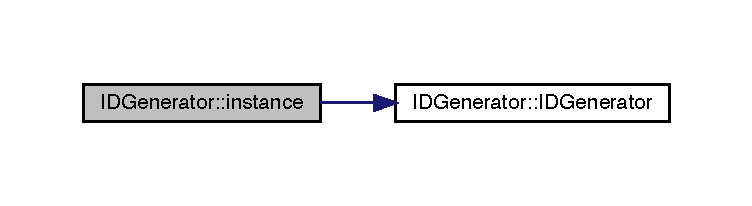
\includegraphics[width=350pt]{class_i_d_generator_ad852c6dadc89e1020e4b3932f5a97bb3_cgraph}
\end{center}
\end{figure}
\mbox{\Hypertarget{class_i_d_generator_a99d8cabb2ec6a17888a8ccbe9c85fee0}\label{class_i_d_generator_a99d8cabb2ec6a17888a8ccbe9c85fee0}} 
\index{I\+D\+Generator@{I\+D\+Generator}!next@{next}}
\index{next@{next}!I\+D\+Generator@{I\+D\+Generator}}
\subsubsection{\texorpdfstring{next()}{next()}}
{\footnotesize\ttfamily unsigned long I\+D\+Generator\+::next (\begin{DoxyParamCaption}{ }\end{DoxyParamCaption})\hspace{0.3cm}{\ttfamily [inline]}}

Generates the next unique identifier. \begin{DoxyReturn}{Returns}
a unique identifier. 
\end{DoxyReturn}


\subsection{Member Data Documentation}
\mbox{\Hypertarget{class_i_d_generator_ad0400380525f694b23ff675f4f170893}\label{class_i_d_generator_ad0400380525f694b23ff675f4f170893}} 
\index{I\+D\+Generator@{I\+D\+Generator}!m\+\_\+id@{m\+\_\+id}}
\index{m\+\_\+id@{m\+\_\+id}!I\+D\+Generator@{I\+D\+Generator}}
\subsubsection{\texorpdfstring{m\+\_\+id}{m\_id}}
{\footnotesize\ttfamily unsigned long I\+D\+Generator\+::m\+\_\+id\hspace{0.3cm}{\ttfamily [private]}}

\mbox{\Hypertarget{class_i_d_generator_a316bacdda67f4cf9bf73fcbd9bf94245}\label{class_i_d_generator_a316bacdda67f4cf9bf73fcbd9bf94245}} 
\index{I\+D\+Generator@{I\+D\+Generator}!m\+\_\+instance@{m\+\_\+instance}}
\index{m\+\_\+instance@{m\+\_\+instance}!I\+D\+Generator@{I\+D\+Generator}}
\subsubsection{\texorpdfstring{m\+\_\+instance}{m\_instance}}
{\footnotesize\ttfamily \hyperlink{class_i_d_generator}{I\+D\+Generator}$\ast$ I\+D\+Generator\+::m\+\_\+instance\hspace{0.3cm}{\ttfamily [static]}, {\ttfamily [private]}}



The documentation for this class was generated from the following file\+:\begin{DoxyCompactItemize}
\item 
include/\hyperlink{_i_d_generator_8h}{I\+D\+Generator.\+h}\end{DoxyCompactItemize}

\section{Immovable\+Agent Class Reference}
\label{class_immovable_agent}\index{Immovable\+Agent@{Immovable\+Agent}}


{\ttfamily \#include $<$Immovable\+Agent.\+h$>$}



Inheritance diagram for Immovable\+Agent\+:
% FIG 0


Collaboration diagram for Immovable\+Agent\+:
% FIG 1
\subsection*{Public Member Functions}
\begin{DoxyCompactItemize}
\item 
\textbf{ Immovable\+Agent} (\textbf{ Map} $\ast$m, long id, Point $\ast$initial\+Position, \textbf{ Clock} $\ast$clock)
\item 
virtual \textbf{ $\sim$\+Immovable\+Agent} ()
\item 
string \textbf{ to\+String} () override
\item 
string \textbf{ get\+Name} () override
\end{DoxyCompactItemize}


\subsection{Detailed Description}


Definition at line 23 of file Immovable\+Agent.\+h.



\subsection{Constructor \& Destructor Documentation}
\mbox{\label{class_immovable_agent_aca3d3a6d6608a1e639a57e84c94e336e}} 
\index{Immovable\+Agent@{Immovable\+Agent}!Immovable\+Agent@{Immovable\+Agent}}
\index{Immovable\+Agent@{Immovable\+Agent}!Immovable\+Agent@{Immovable\+Agent}}
\subsubsection{Immovable\+Agent()}
{\footnotesize\ttfamily Immovable\+Agent\+::\+Immovable\+Agent (\begin{DoxyParamCaption}\item[{\textbf{ Map} $\ast$}]{m,  }\item[{long}]{id,  }\item[{Point $\ast$}]{initial\+Position,  }\item[{\textbf{ Clock} $\ast$}]{clock }\end{DoxyParamCaption})\hspace{0.3cm}{\ttfamily [explicit]}}



Definition at line 17 of file Immovable\+Agent.\+cpp.

\mbox{\label{class_immovable_agent_af8bf8c3a8a322decc4ced38cb1296fee}} 
\index{Immovable\+Agent@{Immovable\+Agent}!````~Immovable\+Agent@{$\sim$\+Immovable\+Agent}}
\index{````~Immovable\+Agent@{$\sim$\+Immovable\+Agent}!Immovable\+Agent@{Immovable\+Agent}}
\subsubsection{$\sim$\+Immovable\+Agent()}
{\footnotesize\ttfamily Immovable\+Agent\+::$\sim$\+Immovable\+Agent (\begin{DoxyParamCaption}{ }\end{DoxyParamCaption})\hspace{0.3cm}{\ttfamily [virtual]}}



Definition at line 22 of file Immovable\+Agent.\+cpp.



\subsection{Member Function Documentation}
\mbox{\label{class_immovable_agent_a35b43ab9d6cd845a0ada5b95784994f0}} 
\index{Immovable\+Agent@{Immovable\+Agent}!get\+Name@{get\+Name}}
\index{get\+Name@{get\+Name}!Immovable\+Agent@{Immovable\+Agent}}
\subsubsection{get\+Name()}
{\footnotesize\ttfamily string Immovable\+Agent\+::get\+Name (\begin{DoxyParamCaption}{ }\end{DoxyParamCaption})\hspace{0.3cm}{\ttfamily [inline]}, {\ttfamily [override]}, {\ttfamily [virtual]}}

This function is used to get the name of the class. It is a pure virtual function, all subclasses implment it and return the actual name of the class. \begin{DoxyReturn}{Returns}
the name of the class. 
\end{DoxyReturn}


Implements \textbf{ Agent} \doxyref{}{p.}{class_agent_aa24682b2e0c8031d0637c156f6bee0e0}.



Definition at line 30 of file Immovable\+Agent.\+h.

\mbox{\label{class_immovable_agent_a94ec08f8c08ec2b4cecf5ef27b00fa32}} 
\index{Immovable\+Agent@{Immovable\+Agent}!to\+String@{to\+String}}
\index{to\+String@{to\+String}!Immovable\+Agent@{Immovable\+Agent}}
\subsubsection{to\+String()}
{\footnotesize\ttfamily string Immovable\+Agent\+::to\+String (\begin{DoxyParamCaption}{ }\end{DoxyParamCaption})\hspace{0.3cm}{\ttfamily [override]}, {\ttfamily [virtual]}}

Builds a string with of the relevant information of the class. It is useful to output on the console or in a file the description of concrete agents. \begin{DoxyReturn}{Returns}
a string representation of the class content. The values of the members are written in this string. 
\end{DoxyReturn}


Implements \textbf{ Agent} \doxyref{}{p.}{class_agent_a530b76f9163b2b8c19e7cdf8065888ac}.



Definition at line 26 of file Immovable\+Agent.\+cpp.



References Locatable\+Agent\+::to\+String().



Referenced by Antenna\+::to\+String().

Here is the call graph for this function\+:
% FIG 2


The documentation for this class was generated from the following files\+:\begin{DoxyCompactItemize}
\item 
include/\textbf{ Immovable\+Agent.\+h}\item 
src/\textbf{ Immovable\+Agent.\+cpp}\end{DoxyCompactItemize}

\section{Input\+Parser Class Reference}
\label{class_input_parser}\index{InputParser@{InputParser}}


{\ttfamily \#include $<$Input\+Parser.\+h$>$}

\subsection*{Public Member Functions}
\begin{DoxyCompactItemize}
\item 
\textbf{ Input\+Parser} (int \&argc, char $\ast$$\ast$argv)
\item 
const string \& \textbf{ get\+Cmd\+Option} (const string \&option) const
\item 
bool \textbf{ cmd\+Option\+Exists} (const string \&option) const
\end{DoxyCompactItemize}
\subsection*{Private Attributes}
\begin{DoxyCompactItemize}
\item 
vector$<$ string $>$ \textbf{ tokens}
\end{DoxyCompactItemize}


\subsection{Detailed Description}


Definition at line 20 of file Input\+Parser.\+h.



\subsection{Constructor \& Destructor Documentation}
\mbox{\label{class_input_parser_af9fa5ead1f28b5294a713410df5b9531}} 
\index{InputParser@{InputParser}!InputParser@{InputParser}}
\index{InputParser@{InputParser}!InputParser@{InputParser}}
\subsubsection{InputParser()}
{\footnotesize\ttfamily Input\+Parser\+::\+Input\+Parser (\begin{DoxyParamCaption}\item[{int \&}]{argc,  }\item[{char $\ast$$\ast$}]{argv }\end{DoxyParamCaption})}



Definition at line 14 of file Input\+Parser.\+cpp.



References tokens.



\subsection{Member Function Documentation}
\mbox{\label{class_input_parser_ad3d06a9c59e91f425295bdc8408e0544}} 
\index{InputParser@{InputParser}!cmdOptionExists@{cmdOptionExists}}
\index{cmdOptionExists@{cmdOptionExists}!InputParser@{InputParser}}
\subsubsection{cmdOptionExists()}
{\footnotesize\ttfamily bool Input\+Parser\+::cmd\+Option\+Exists (\begin{DoxyParamCaption}\item[{const string \&}]{option }\end{DoxyParamCaption}) const}



Definition at line 29 of file Input\+Parser.\+cpp.



References tokens.

\mbox{\label{class_input_parser_a494c1de8c06fbb5a88343686e36fbf50}} 
\index{InputParser@{InputParser}!getCmdOption@{getCmdOption}}
\index{getCmdOption@{getCmdOption}!InputParser@{InputParser}}
\subsubsection{getCmdOption()}
{\footnotesize\ttfamily const string \& Input\+Parser\+::get\+Cmd\+Option (\begin{DoxyParamCaption}\item[{const string \&}]{option }\end{DoxyParamCaption}) const}



Definition at line 19 of file Input\+Parser.\+cpp.



References tokens.



\subsection{Member Data Documentation}
\mbox{\label{class_input_parser_a4bd1105d6fc64bd0e825dc2e34515d75}} 
\index{InputParser@{InputParser}!tokens@{tokens}}
\index{tokens@{tokens}!InputParser@{InputParser}}
\subsubsection{tokens}
{\footnotesize\ttfamily vector$<$string$>$ Input\+Parser\+::tokens\hspace{0.3cm}{\ttfamily [private]}}



Definition at line 26 of file Input\+Parser.\+h.



Referenced by cmd\+Option\+Exists(), get\+Cmd\+Option(), and Input\+Parser().



The documentation for this class was generated from the following files\+:\begin{DoxyCompactItemize}
\item 
include/\textbf{ Input\+Parser.\+h}\item 
src/\textbf{ Input\+Parser.\+cpp}\end{DoxyCompactItemize}

\section{Locatable\+Agent Class Reference}
\label{class_locatable_agent}\index{LocatableAgent@{LocatableAgent}}


{\ttfamily \#include $<$Locatable\+Agent.\+h$>$}

Inheritance diagram for Locatable\+Agent\+:\begin{figure}[H]
\begin{center}
\leavevmode
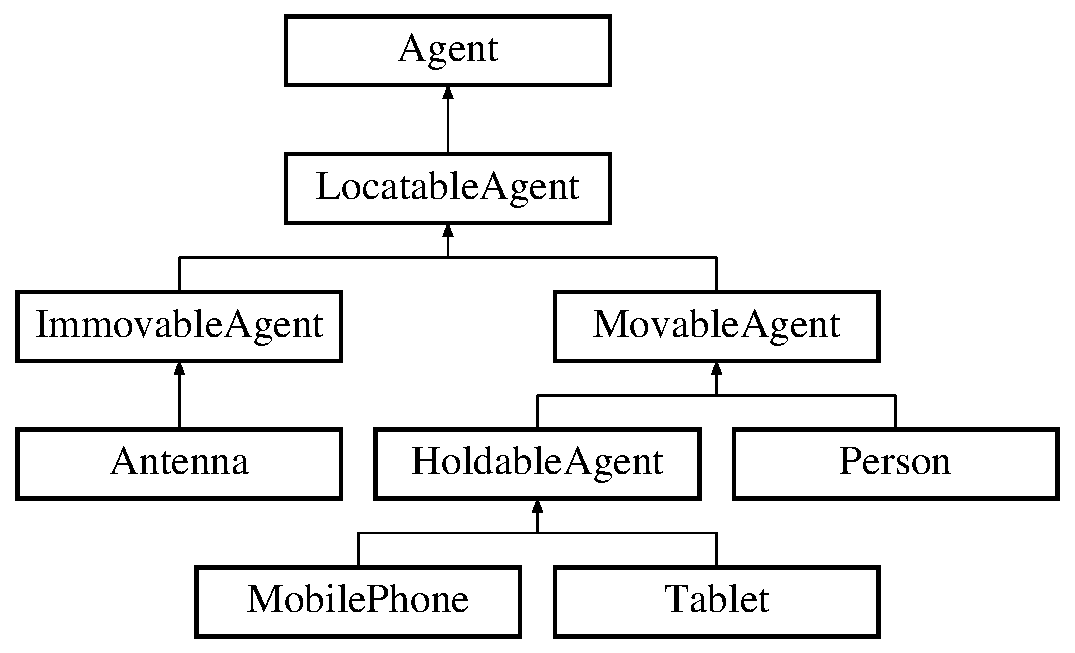
\includegraphics[height=5.000000cm]{class_locatable_agent}
\end{center}
\end{figure}
\subsection*{Public Member Functions}
\begin{DoxyCompactItemize}
\item 
\textbf{ Locatable\+Agent} (\textbf{ Map} $\ast$m, long id, Point $\ast$init\+Location, \textbf{ Clock} $\ast$clock)
\item 
virtual \textbf{ $\sim$\+Locatable\+Agent} ()
\item 
string \textbf{ get\+Name} () override
\item 
string \textbf{ to\+String} () override
\item 
virtual Point $\ast$ \textbf{ get\+Location} () const
\item 
virtual void \textbf{ set\+Location} (Point $\ast$location)
\item 
string \textbf{ dump\+Location} ()
\end{DoxyCompactItemize}
\subsection*{Private Attributes}
\begin{DoxyCompactItemize}
\item 
Point $\ast$ \textbf{ m\+\_\+location}
\end{DoxyCompactItemize}


\subsection{Detailed Description}


Definition at line 21 of file Locatable\+Agent.\+h.



\subsection{Constructor \& Destructor Documentation}
\mbox{\label{class_locatable_agent_ac499b75f07ffa4daf3da16488953533e}} 
\index{LocatableAgent@{LocatableAgent}!LocatableAgent@{LocatableAgent}}
\index{LocatableAgent@{LocatableAgent}!LocatableAgent@{LocatableAgent}}
\subsubsection{LocatableAgent()}
{\footnotesize\ttfamily Locatable\+Agent\+::\+Locatable\+Agent (\begin{DoxyParamCaption}\item[{\textbf{ Map} $\ast$}]{m,  }\item[{long}]{id,  }\item[{Point $\ast$}]{init\+Location,  }\item[{\textbf{ Clock} $\ast$}]{clock }\end{DoxyParamCaption})\hspace{0.3cm}{\ttfamily [explicit]}}



Definition at line 20 of file Locatable\+Agent.\+cpp.



References m\+\_\+location.

\mbox{\label{class_locatable_agent_a6a088f1e2c16a0b52e4a630868d4eae6}} 
\index{LocatableAgent@{LocatableAgent}!````~LocatableAgent@{$\sim$LocatableAgent}}
\index{````~LocatableAgent@{$\sim$LocatableAgent}!LocatableAgent@{LocatableAgent}}
\subsubsection{$\sim$LocatableAgent()}
{\footnotesize\ttfamily Locatable\+Agent\+::$\sim$\+Locatable\+Agent (\begin{DoxyParamCaption}{ }\end{DoxyParamCaption})\hspace{0.3cm}{\ttfamily [virtual]}}



Definition at line 26 of file Locatable\+Agent.\+cpp.



\subsection{Member Function Documentation}
\mbox{\label{class_locatable_agent_ab4436577328ce536ccba55d3068b2cf4}} 
\index{LocatableAgent@{LocatableAgent}!dumpLocation@{dumpLocation}}
\index{dumpLocation@{dumpLocation}!LocatableAgent@{LocatableAgent}}
\subsubsection{dumpLocation()}
{\footnotesize\ttfamily string Locatable\+Agent\+::dump\+Location (\begin{DoxyParamCaption}{ }\end{DoxyParamCaption})}



Definition at line 49 of file Locatable\+Agent.\+cpp.



References Agent\+::get\+Clock(), Clock\+::get\+Current\+Time(), Agent\+::get\+Id(), and get\+Location().



Referenced by World\+::run\+Simulation().

\mbox{\label{class_locatable_agent_a2392d365653e71cc35029fdebbfe18d9}} 
\index{LocatableAgent@{LocatableAgent}!getLocation@{getLocation}}
\index{getLocation@{getLocation}!LocatableAgent@{LocatableAgent}}
\subsubsection{getLocation()}
{\footnotesize\ttfamily Point $\ast$ Locatable\+Agent\+::get\+Location (\begin{DoxyParamCaption}{ }\end{DoxyParamCaption}) const\hspace{0.3cm}{\ttfamily [virtual]}}



Definition at line 31 of file Locatable\+Agent.\+cpp.



References m\+\_\+location.



Referenced by Antenna\+::compute\+Power(), Antenna\+::compute\+Signal\+Quality(), dump\+Location(), Tablet\+::move(), Person\+::move(), Person\+::random\+Walk(), Antenna\+::register\+Event(), Holdable\+Agent\+::set\+Holder(), to\+String(), and Mobile\+Phone\+::try\+Connect\+Naive\+Algorithm().

\mbox{\label{class_locatable_agent_ae2b9a1bd2e207a9aac95f4d13a17a9f9}} 
\index{LocatableAgent@{LocatableAgent}!getName@{getName}}
\index{getName@{getName}!LocatableAgent@{LocatableAgent}}
\subsubsection{getName()}
{\footnotesize\ttfamily string Locatable\+Agent\+::get\+Name (\begin{DoxyParamCaption}{ }\end{DoxyParamCaption})\hspace{0.3cm}{\ttfamily [inline]}, {\ttfamily [override]}, {\ttfamily [virtual]}}

This function is used to get the name of the class. It is a pure virtual function, all subclasses implment it and return the actual name of the class. \begin{DoxyReturn}{Returns}
the name of the class. 
\end{DoxyReturn}


Implements \textbf{ Agent} \doxyref{}{p.}{class_agent_aa24682b2e0c8031d0637c156f6bee0e0}.



Reimplemented in \textbf{ Person} \doxyref{}{p.}{class_person_a41c6a0cd763dc154841346e69f2d4b3e}, \textbf{ Movable\+Agent} \doxyref{}{p.}{class_movable_agent_af36b0e49e477cfcc60d801c11166a4f0}, \textbf{ Mobile\+Phone} \doxyref{}{p.}{class_mobile_phone_aa4f050bb755994fadfeab94c1f2147f7}, and \textbf{ Tablet} \doxyref{}{p.}{class_tablet_a2cac00cd9efca5b8adeff28ae5827970}.



Definition at line 27 of file Locatable\+Agent.\+h.

\mbox{\label{class_locatable_agent_a4185a45957d529a7f57d19ea294cae81}} 
\index{LocatableAgent@{LocatableAgent}!setLocation@{setLocation}}
\index{setLocation@{setLocation}!LocatableAgent@{LocatableAgent}}
\subsubsection{setLocation()}
{\footnotesize\ttfamily void Locatable\+Agent\+::set\+Location (\begin{DoxyParamCaption}\item[{Point $\ast$}]{location }\end{DoxyParamCaption})\hspace{0.3cm}{\ttfamily [virtual]}}



Reimplemented in \textbf{ Person} \doxyref{}{p.}{class_person_a2b31d3b9e0d9ed3b583d6d8d4c632518}, and \textbf{ Holdable\+Agent} \doxyref{}{p.}{class_holdable_agent_aec98d2fe325b48d9a84ad3dad44700e0}.



Definition at line 35 of file Locatable\+Agent.\+cpp.



References m\+\_\+location.



Referenced by Antenna\+::\+Antenna(), Holdable\+Agent\+::set\+Location(), and Person\+::set\+Location().

\mbox{\label{class_locatable_agent_a593b8f4eb5d0a812b725726c35335193}} 
\index{LocatableAgent@{LocatableAgent}!toString@{toString}}
\index{toString@{toString}!LocatableAgent@{LocatableAgent}}
\subsubsection{toString()}
{\footnotesize\ttfamily string Locatable\+Agent\+::to\+String (\begin{DoxyParamCaption}{ }\end{DoxyParamCaption})\hspace{0.3cm}{\ttfamily [override]}, {\ttfamily [virtual]}}

Builds a string with of the relevant information of the class. It is useful to output on the console or in a file the description of concrete agents. \begin{DoxyReturn}{Returns}
a string representation of the class content. The values of the members are written in this string. 
\end{DoxyReturn}


Implements \textbf{ Agent} \doxyref{}{p.}{class_agent_a530b76f9163b2b8c19e7cdf8065888ac}.



Reimplemented in \textbf{ Person} \doxyref{}{p.}{class_person_ac39b105901a2d4ce38ff5b548b1c349e}, \textbf{ Movable\+Agent} \doxyref{}{p.}{class_movable_agent_aa8a8424a9513e0d57f7d4b94e7a49552}, \textbf{ Mobile\+Phone} \doxyref{}{p.}{class_mobile_phone_a3e4bf0a37331042084ae703666f8fb7c}, and \textbf{ Tablet} \doxyref{}{p.}{class_tablet_a90880cd8f4a4afd451645e6e1dc86c5b}.



Definition at line 39 of file Locatable\+Agent.\+cpp.



References Agent\+::get\+Id(), get\+Location(), and m\+\_\+location.



Referenced by Immovable\+Agent\+::to\+String(), and Movable\+Agent\+::to\+String().



\subsection{Member Data Documentation}
\mbox{\label{class_locatable_agent_a2a76ba315733ab26f19229a71071704d}} 
\index{LocatableAgent@{LocatableAgent}!m\_location@{m\_location}}
\index{m\_location@{m\_location}!LocatableAgent@{LocatableAgent}}
\subsubsection{m\_location}
{\footnotesize\ttfamily Point$\ast$ Locatable\+Agent\+::m\+\_\+location\hspace{0.3cm}{\ttfamily [private]}}



Definition at line 41 of file Locatable\+Agent.\+h.



Referenced by get\+Location(), Locatable\+Agent(), set\+Location(), and to\+String().



The documentation for this class was generated from the following files\+:\begin{DoxyCompactItemize}
\item 
include/\textbf{ Locatable\+Agent.\+h}\item 
src/\textbf{ Locatable\+Agent.\+cpp}\end{DoxyCompactItemize}

\hypertarget{class_map}{}\section{Map Class Reference}
\label{class_map}\index{Map@{Map}}


{\ttfamily \#include $<$Map.\+h$>$}



Collaboration diagram for Map\+:\nopagebreak
\begin{figure}[H]
\begin{center}
\leavevmode
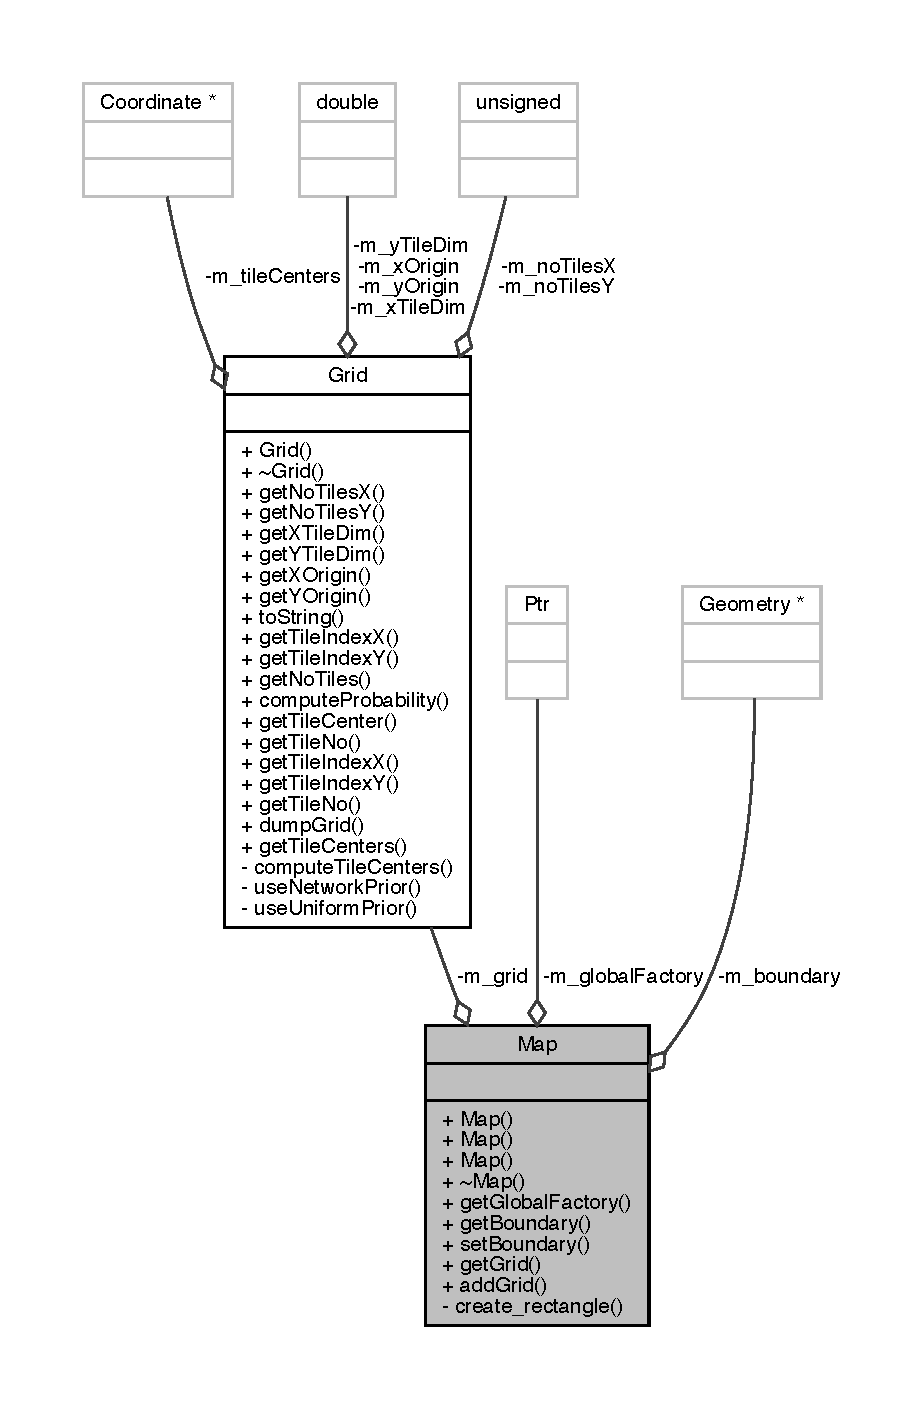
\includegraphics[width=350pt]{class_map__coll__graph}
\end{center}
\end{figure}
\subsection*{Public Member Functions}
\begin{DoxyCompactItemize}
\item 
\mbox{\hyperlink{class_map_a0f5ad0fd4563497b4214038cbca8b582}{Map}} ()
\item 
\mbox{\hyperlink{class_map_a4c9545a0252613e2a6808932fe83f9ad}{Map}} (double llX, double llY, double width, double height)
\item 
\mbox{\hyperlink{class_map_ab8beab7a7dce782a23db740cd7132552}{Map}} (string wkt\+File)
\item 
virtual \mbox{\hyperlink{class_map_ac1ab46138aa61acd0a58b1fd21e0df37}{$\sim$\+Map}} ()
\item 
const Geometry\+Factory\+::\+Ptr \& \mbox{\hyperlink{class_map_a69bd639b05daa393b051c76f0dc4af7c}{get\+Global\+Factory}} () const
\item 
Geometry $\ast$ \mbox{\hyperlink{class_map_a74dd5445ed90bea2a9cc3240bc23f1bc}{get\+Boundary}} () const
\item 
void \mbox{\hyperlink{class_map_acede2ccba9bf0f987f3dde8c332bec17}{set\+Boundary}} (Geometry $\ast$boundary)
\item 
const \mbox{\hyperlink{class_grid}{Grid}} $\ast$ \mbox{\hyperlink{class_map_aa9bf1c29b844f3b7fbf7a3153c24fef0}{get\+Grid}} () const
\item 
void \mbox{\hyperlink{class_map_aa3dba78a0b52b304c39d1fa6bff71b00}{add\+Grid}} (double dim\+TileX, double dim\+TileY)
\end{DoxyCompactItemize}
\subsection*{Private Member Functions}
\begin{DoxyCompactItemize}
\item 
Polygon $\ast$ \mbox{\hyperlink{class_map_a36539152d451138361d82469218b4661}{create\+\_\+rectangle}} (double llX, double llY, double width, double height)
\end{DoxyCompactItemize}
\subsection*{Private Attributes}
\begin{DoxyCompactItemize}
\item 
Geometry\+Factory\+::\+Ptr \mbox{\hyperlink{class_map_ac5f30e6c144955a3638192495fd7d843}{m\+\_\+global\+Factory}}
\item 
Geometry $\ast$ \mbox{\hyperlink{class_map_af2c95561cb4ff3b9950240351cf4303c}{m\+\_\+boundary}}
\item 
\mbox{\hyperlink{class_grid}{Grid}} $\ast$ \mbox{\hyperlink{class_map_a0fc16621dbe307d36170c3a96b24b7d9}{m\+\_\+grid}}
\end{DoxyCompactItemize}


\subsection{Detailed Description}
This is the map where the simulation takes place. It could be a simple rectangle or any kind of geometry object(s) read from a wkt file. The map has a boundary that is implemented as a Geometry object, a factory object of Geometry\+Factory type used to create other objects. All geometric and geographic features of the simulator uses the G\+E\+OS library. G\+E\+OS is an open source C++ library which is just a port to C++ of the well known Java Topology Suite. 

\subsection{Constructor \& Destructor Documentation}
\mbox{\Hypertarget{class_map_a0f5ad0fd4563497b4214038cbca8b582}\label{class_map_a0f5ad0fd4563497b4214038cbca8b582}} 
\index{Map@{Map}!Map@{Map}}
\index{Map@{Map}!Map@{Map}}
\subsubsection{\texorpdfstring{Map()}{Map()}\hspace{0.1cm}{\footnotesize\ttfamily [1/3]}}
{\footnotesize\ttfamily Map\+::\+Map (\begin{DoxyParamCaption}{ }\end{DoxyParamCaption})}

Creates a map with a null boundary. The user may set the boundary later, using \mbox{\hyperlink{class_map_acede2ccba9bf0f987f3dde8c332bec17}{set\+Boundary()}} method. \mbox{\Hypertarget{class_map_a4c9545a0252613e2a6808932fe83f9ad}\label{class_map_a4c9545a0252613e2a6808932fe83f9ad}} 
\index{Map@{Map}!Map@{Map}}
\index{Map@{Map}!Map@{Map}}
\subsubsection{\texorpdfstring{Map()}{Map()}\hspace{0.1cm}{\footnotesize\ttfamily [2/3]}}
{\footnotesize\ttfamily Map\+::\+Map (\begin{DoxyParamCaption}\item[{double}]{llX,  }\item[{double}]{llY,  }\item[{double}]{width,  }\item[{double}]{height }\end{DoxyParamCaption})}

Build a simple map of a rectangular shape. 
\begin{DoxyParams}{Parameters}
{\em llX} & X coordinate of the bottom left corner of the rectangle. \\
\hline
{\em llY} & Y coordinate of the bottom left corner of the rectangle. \\
\hline
{\em width} & the width of the rectangle. \\
\hline
{\em height} & the height of the rectangle. \\
\hline
\end{DoxyParams}
\mbox{\Hypertarget{class_map_ab8beab7a7dce782a23db740cd7132552}\label{class_map_ab8beab7a7dce782a23db740cd7132552}} 
\index{Map@{Map}!Map@{Map}}
\index{Map@{Map}!Map@{Map}}
\subsubsection{\texorpdfstring{Map()}{Map()}\hspace{0.1cm}{\footnotesize\ttfamily [3/3]}}
{\footnotesize\ttfamily Map\+::\+Map (\begin{DoxyParamCaption}\item[{string}]{wkt\+File }\end{DoxyParamCaption})}

Builds a map reading it from a .wkt file. 
\begin{DoxyParams}{Parameters}
{\em wkt\+File} & the name of the .wkt file that contains the description of the map. Currently, the first row of this file should contain the external boundary geometry of the map. \\
\hline
\end{DoxyParams}
\mbox{\Hypertarget{class_map_ac1ab46138aa61acd0a58b1fd21e0df37}\label{class_map_ac1ab46138aa61acd0a58b1fd21e0df37}} 
\index{Map@{Map}!````~Map@{$\sim$Map}}
\index{````~Map@{$\sim$Map}!Map@{Map}}
\subsubsection{\texorpdfstring{$\sim$Map()}{~Map()}}
{\footnotesize\ttfamily virtual Map\+::$\sim$\+Map (\begin{DoxyParamCaption}{ }\end{DoxyParamCaption})\hspace{0.3cm}{\ttfamily [virtual]}}

Default destructor 

\subsection{Member Function Documentation}
\mbox{\Hypertarget{class_map_aa3dba78a0b52b304c39d1fa6bff71b00}\label{class_map_aa3dba78a0b52b304c39d1fa6bff71b00}} 
\index{Map@{Map}!addGrid@{addGrid}}
\index{addGrid@{addGrid}!Map@{Map}}
\subsubsection{\texorpdfstring{addGrid()}{addGrid()}}
{\footnotesize\ttfamily void Map\+::add\+Grid (\begin{DoxyParamCaption}\item[{double}]{dim\+TileX,  }\item[{double}]{dim\+TileY }\end{DoxyParamCaption})}

Adds a \mbox{\hyperlink{class_grid}{Grid}} that overlaps this \mbox{\hyperlink{class_map}{Map}} objects. 
\begin{DoxyParams}{Parameters}
{\em dim\+TileX} & the dimension on OX of a tile of the \mbox{\hyperlink{class_grid}{Grid}} object. \\
\hline
{\em dim\+TileY} & the dimension on OY of a tile of the \mbox{\hyperlink{class_grid}{Grid}} object. \\
\hline
\end{DoxyParams}
\mbox{\Hypertarget{class_map_a36539152d451138361d82469218b4661}\label{class_map_a36539152d451138361d82469218b4661}} 
\index{Map@{Map}!create\_rectangle@{create\_rectangle}}
\index{create\_rectangle@{create\_rectangle}!Map@{Map}}
\subsubsection{\texorpdfstring{create\_rectangle()}{create\_rectangle()}}
{\footnotesize\ttfamily Polygon$\ast$ Map\+::create\+\_\+rectangle (\begin{DoxyParamCaption}\item[{double}]{llX,  }\item[{double}]{llY,  }\item[{double}]{width,  }\item[{double}]{height }\end{DoxyParamCaption})\hspace{0.3cm}{\ttfamily [private]}}

\mbox{\Hypertarget{class_map_a74dd5445ed90bea2a9cc3240bc23f1bc}\label{class_map_a74dd5445ed90bea2a9cc3240bc23f1bc}} 
\index{Map@{Map}!getBoundary@{getBoundary}}
\index{getBoundary@{getBoundary}!Map@{Map}}
\subsubsection{\texorpdfstring{getBoundary()}{getBoundary()}}
{\footnotesize\ttfamily Geometry$\ast$ Map\+::get\+Boundary (\begin{DoxyParamCaption}{ }\end{DoxyParamCaption}) const}

Returns a pointer to the Geometry object that represents the external boundary of the map. \begin{DoxyReturn}{Returns}
a pointer to the Geometry object that represents the external boundary of the map. 
\end{DoxyReturn}
\mbox{\Hypertarget{class_map_a69bd639b05daa393b051c76f0dc4af7c}\label{class_map_a69bd639b05daa393b051c76f0dc4af7c}} 
\index{Map@{Map}!getGlobalFactory@{getGlobalFactory}}
\index{getGlobalFactory@{getGlobalFactory}!Map@{Map}}
\subsubsection{\texorpdfstring{getGlobalFactory()}{getGlobalFactory()}}
{\footnotesize\ttfamily const Geometry\+Factory\+::\+Ptr\& Map\+::get\+Global\+Factory (\begin{DoxyParamCaption}{ }\end{DoxyParamCaption}) const}

Returns a pointer to the Geometry\+Factory object which is a factory object used to create other geometric objects. The G\+E\+OS library allows users to create geometric objects only using this factory, all the constructors are made private. \begin{DoxyReturn}{Returns}
a pointer to the Geometry\+Factory object used to create other geometric objects. 
\end{DoxyReturn}
\mbox{\Hypertarget{class_map_aa9bf1c29b844f3b7fbf7a3153c24fef0}\label{class_map_aa9bf1c29b844f3b7fbf7a3153c24fef0}} 
\index{Map@{Map}!getGrid@{getGrid}}
\index{getGrid@{getGrid}!Map@{Map}}
\subsubsection{\texorpdfstring{getGrid()}{getGrid()}}
{\footnotesize\ttfamily const \mbox{\hyperlink{class_grid}{Grid}}$\ast$ Map\+::get\+Grid (\begin{DoxyParamCaption}{ }\end{DoxyParamCaption}) const}

Returns a pointer to the \mbox{\hyperlink{class_grid}{Grid}} object associated with this \mbox{\hyperlink{class_map}{Map}}. After creation of a \mbox{\hyperlink{class_map}{Map}} the user should associate a \mbox{\hyperlink{class_grid}{Grid}} that overlaps this \mbox{\hyperlink{class_map}{Map}}. The gird is used to compute the probability of the localization of different events during the simulation. \begin{DoxyReturn}{Returns}
a pointer the \mbox{\hyperlink{class_grid}{Grid}} object associated with this \mbox{\hyperlink{class_map}{Map}}. 
\end{DoxyReturn}
\mbox{\Hypertarget{class_map_acede2ccba9bf0f987f3dde8c332bec17}\label{class_map_acede2ccba9bf0f987f3dde8c332bec17}} 
\index{Map@{Map}!setBoundary@{setBoundary}}
\index{setBoundary@{setBoundary}!Map@{Map}}
\subsubsection{\texorpdfstring{setBoundary()}{setBoundary()}}
{\footnotesize\ttfamily void Map\+::set\+Boundary (\begin{DoxyParamCaption}\item[{Geometry $\ast$}]{boundary }\end{DoxyParamCaption})}

Sets the boundary of the \mbox{\hyperlink{class_map}{Map}} object. 
\begin{DoxyParams}{Parameters}
{\em boundary} & the boundary of the \mbox{\hyperlink{class_map}{Map}} object. \\
\hline
\end{DoxyParams}


\subsection{Member Data Documentation}
\mbox{\Hypertarget{class_map_af2c95561cb4ff3b9950240351cf4303c}\label{class_map_af2c95561cb4ff3b9950240351cf4303c}} 
\index{Map@{Map}!m\_boundary@{m\_boundary}}
\index{m\_boundary@{m\_boundary}!Map@{Map}}
\subsubsection{\texorpdfstring{m\_boundary}{m\_boundary}}
{\footnotesize\ttfamily Geometry$\ast$ Map\+::m\+\_\+boundary\hspace{0.3cm}{\ttfamily [private]}}

\mbox{\Hypertarget{class_map_ac5f30e6c144955a3638192495fd7d843}\label{class_map_ac5f30e6c144955a3638192495fd7d843}} 
\index{Map@{Map}!m\_globalFactory@{m\_globalFactory}}
\index{m\_globalFactory@{m\_globalFactory}!Map@{Map}}
\subsubsection{\texorpdfstring{m\_globalFactory}{m\_globalFactory}}
{\footnotesize\ttfamily Geometry\+Factory\+::\+Ptr Map\+::m\+\_\+global\+Factory\hspace{0.3cm}{\ttfamily [private]}}

\mbox{\Hypertarget{class_map_a0fc16621dbe307d36170c3a96b24b7d9}\label{class_map_a0fc16621dbe307d36170c3a96b24b7d9}} 
\index{Map@{Map}!m\_grid@{m\_grid}}
\index{m\_grid@{m\_grid}!Map@{Map}}
\subsubsection{\texorpdfstring{m\_grid}{m\_grid}}
{\footnotesize\ttfamily \mbox{\hyperlink{class_grid}{Grid}}$\ast$ Map\+::m\+\_\+grid\hspace{0.3cm}{\ttfamily [private]}}



The documentation for this class was generated from the following file\+:\begin{DoxyCompactItemize}
\item 
include/\mbox{\hyperlink{_map_8h}{Map.\+h}}\end{DoxyCompactItemize}

\hypertarget{class_mobile_operator}{}\section{Mobile\+Operator Class Reference}
\label{class_mobile_operator}\index{Mobile\+Operator@{Mobile\+Operator}}


{\ttfamily \#include $<$Mobile\+Operator.\+h$>$}



Inheritance diagram for Mobile\+Operator\+:\nopagebreak
\begin{figure}[H]
\begin{center}
\leavevmode
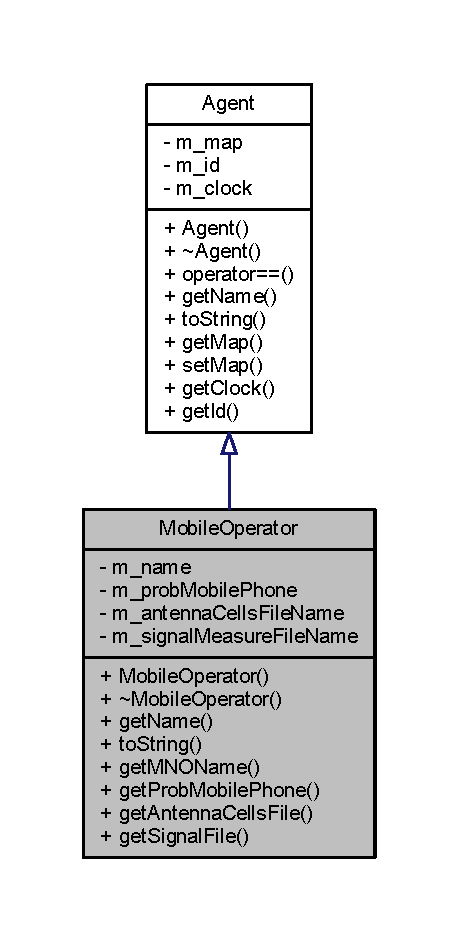
\includegraphics[width=220pt]{class_mobile_operator__inherit__graph}
\end{center}
\end{figure}


Collaboration diagram for Mobile\+Operator\+:\nopagebreak
\begin{figure}[H]
\begin{center}
\leavevmode
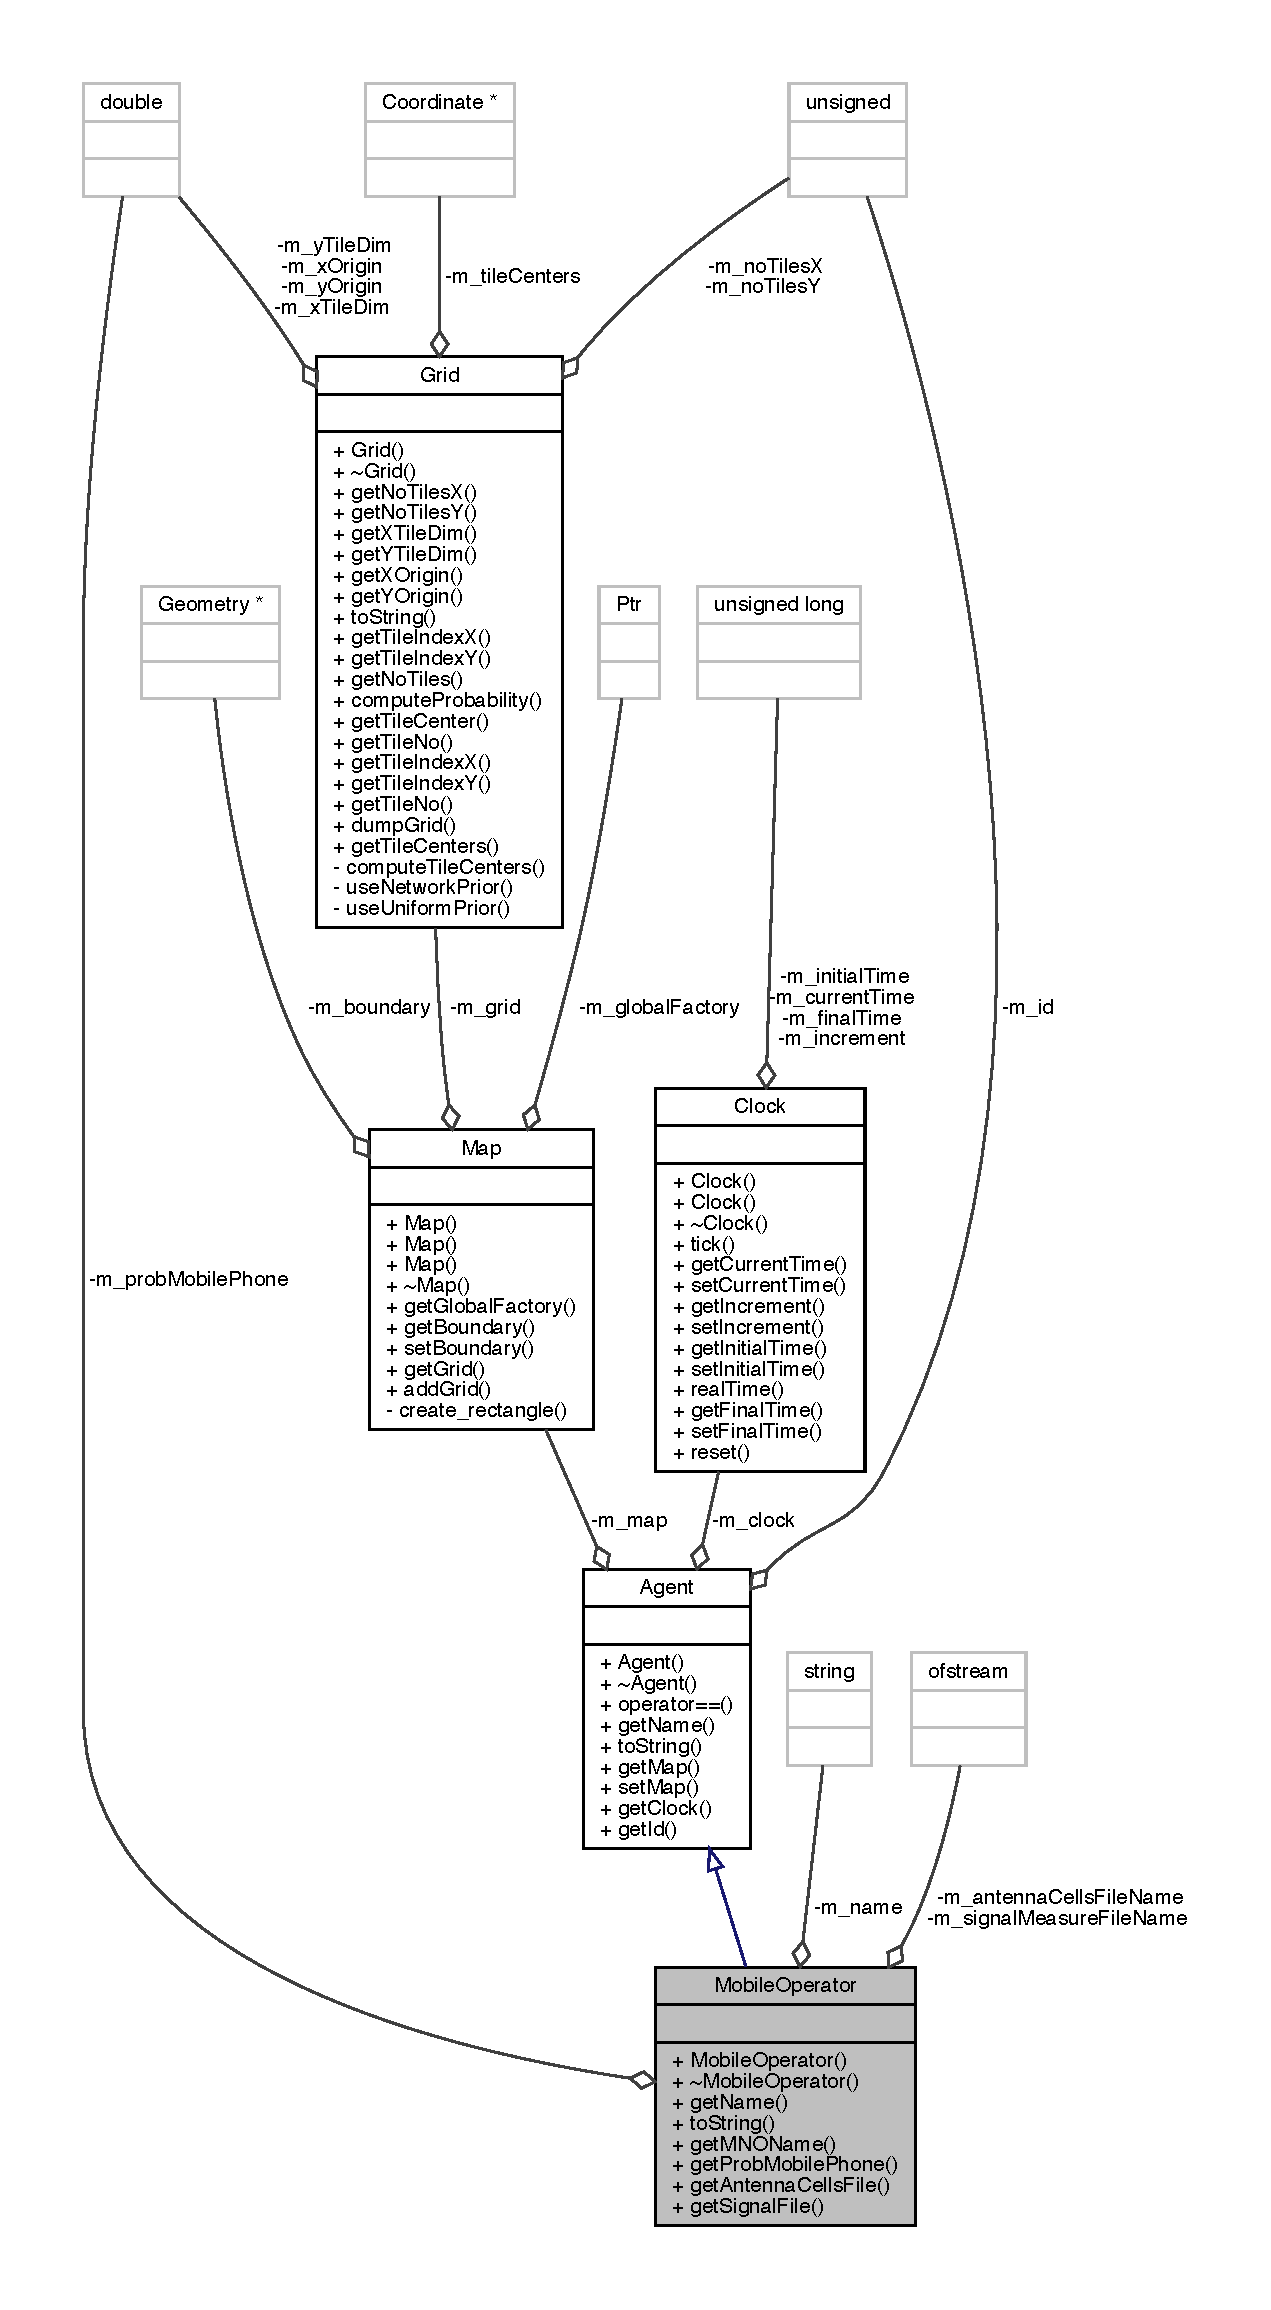
\includegraphics[height=550pt]{class_mobile_operator__coll__graph}
\end{center}
\end{figure}
\subsection*{Public Member Functions}
\begin{DoxyCompactItemize}
\item 
\hyperlink{class_mobile_operator_a8a8ad5fccedc56a31118f248f2aa332f}{Mobile\+Operator} (const \hyperlink{class_map}{Map} $\ast$m, const unsigned long id, const \hyperlink{class_clock}{Clock} $\ast$clock, const char $\ast$name, const double prob\+Mobile\+Phone)
\item 
virtual \hyperlink{class_mobile_operator_af77920475ff630755355f67b8f5f2708}{$\sim$\+Mobile\+Operator} ()
\item 
const string \hyperlink{class_mobile_operator_a2b4538d96f7aa898e6e470411d40cbf7}{get\+Name} () const override
\item 
const string \hyperlink{class_mobile_operator_aa83724a149499ef10678ad651a5b40df}{to\+String} () const override
\item 
const string \hyperlink{class_mobile_operator_a003a5d91f543eaf5ff11894bd462ac77}{get\+M\+N\+O\+Name} () const
\item 
const double \hyperlink{class_mobile_operator_afe59edb4ba22cea7fab968fdd1e2ce31}{get\+Prob\+Mobile\+Phone} () const
\item 
ofstream \& \hyperlink{class_mobile_operator_ae6aa3043d946fa97eba7032b9707e52a}{get\+Antenna\+Cells\+File} ()
\item 
ofstream \& \hyperlink{class_mobile_operator_ac39217182fd0ce7ef5da3b9018bcb965}{get\+Signal\+File} ()
\end{DoxyCompactItemize}
\subsection*{Private Attributes}
\begin{DoxyCompactItemize}
\item 
const string \hyperlink{class_mobile_operator_adc9bb6e834adbaf7f85ad7cf9e4c9bec}{m\+\_\+name}
\item 
const double \hyperlink{class_mobile_operator_a4061b50b15ec5499d57ef0e85687c1a2}{m\+\_\+prob\+Mobile\+Phone}
\item 
ofstream \hyperlink{class_mobile_operator_abd11e27d3ed1273be761a55da1549fa4}{m\+\_\+antenna\+Cells\+File\+Name}
\item 
ofstream \hyperlink{class_mobile_operator_af9c02c4088656c0f21ecc93b7023e776}{m\+\_\+signal\+Measure\+File\+Name}
\end{DoxyCompactItemize}


\subsection{Detailed Description}
This class represents a Mobile Operator company. Currently a simulation can be run with 1 or 2 mobile operators. A mobile operator own a set of antennas and has a set of mobile phone subscribed. 

\subsection{Constructor \& Destructor Documentation}
\mbox{\Hypertarget{class_mobile_operator_a8a8ad5fccedc56a31118f248f2aa332f}\label{class_mobile_operator_a8a8ad5fccedc56a31118f248f2aa332f}} 
\index{Mobile\+Operator@{Mobile\+Operator}!Mobile\+Operator@{Mobile\+Operator}}
\index{Mobile\+Operator@{Mobile\+Operator}!Mobile\+Operator@{Mobile\+Operator}}
\subsubsection{\texorpdfstring{Mobile\+Operator()}{MobileOperator()}}
{\footnotesize\ttfamily Mobile\+Operator\+::\+Mobile\+Operator (\begin{DoxyParamCaption}\item[{const \hyperlink{class_map}{Map} $\ast$}]{m,  }\item[{const unsigned long}]{id,  }\item[{const \hyperlink{class_clock}{Clock} $\ast$}]{clock,  }\item[{const char $\ast$}]{name,  }\item[{const double}]{prob\+Mobile\+Phone }\end{DoxyParamCaption})}

Constructor of this class. It builds a \hyperlink{class_mobile_operator}{Mobile\+Operator} object with the characteristics provided by user through parameters. It builds a string representing the name of the file where the coverage area of all the antennas that belong to this \hyperlink{class_mobile_operator}{Mobile\+Operator} are saved in .csv format and then open this file and writes the header of the file. The name of this file is built concatenating \char`\"{}\+Antenna\+Cells\+\_\+\char`\"{} with the name of the Mobile Operator. The extension of the file is \char`\"{}.\+csv\char`\"{}. A line of this file contains the antenna id followed by a wkt text representing the coverage area of antenna. It also builds another string representing the name of a file where the signal quality values for all antennas that belong to this \hyperlink{class_mobile_operator}{Mobile\+Operator} are saved. The signal quality is computed in the center of each tile of the \hyperlink{class_grid}{Grid} object set for a simulation. The file is opened and then it writes the header of the file. The name of this file is built concatenating \char`\"{}\+Signal\+Quality\+\_\+\char`\"{} with the name of the Mobile Operator. The extension of the file is \char`\"{}.\+csv\char`\"{}. A line of this file contains the antenna id followed by a set of values for the signal quality computed in the center of each tile of the grid. 
\begin{DoxyParams}{Parameters}
{\em m} & a pointer to a \hyperlink{class_map}{Map} object where the simulation take place. \\
\hline
{\em id} & the id of the \hyperlink{class_mobile_operator}{Mobile\+Operator} object. \\
\hline
{\em clock} & a pointer to a \hyperlink{class_clock}{Clock} object used for a simulation. \\
\hline
{\em name} & the name of the Mobile Operator. \\
\hline
{\em prob\+Mobile\+Phone} & represents the probability that a person will have a cell phone at this company. \\
\hline
\end{DoxyParams}
\mbox{\Hypertarget{class_mobile_operator_af77920475ff630755355f67b8f5f2708}\label{class_mobile_operator_af77920475ff630755355f67b8f5f2708}} 
\index{Mobile\+Operator@{Mobile\+Operator}!````~Mobile\+Operator@{$\sim$\+Mobile\+Operator}}
\index{````~Mobile\+Operator@{$\sim$\+Mobile\+Operator}!Mobile\+Operator@{Mobile\+Operator}}
\subsubsection{\texorpdfstring{$\sim$\+Mobile\+Operator()}{~MobileOperator()}}
{\footnotesize\ttfamily virtual Mobile\+Operator\+::$\sim$\+Mobile\+Operator (\begin{DoxyParamCaption}{ }\end{DoxyParamCaption})\hspace{0.3cm}{\ttfamily [virtual]}}

Default destructor. 

\subsection{Member Function Documentation}
\mbox{\Hypertarget{class_mobile_operator_ae6aa3043d946fa97eba7032b9707e52a}\label{class_mobile_operator_ae6aa3043d946fa97eba7032b9707e52a}} 
\index{Mobile\+Operator@{Mobile\+Operator}!get\+Antenna\+Cells\+File@{get\+Antenna\+Cells\+File}}
\index{get\+Antenna\+Cells\+File@{get\+Antenna\+Cells\+File}!Mobile\+Operator@{Mobile\+Operator}}
\subsubsection{\texorpdfstring{get\+Antenna\+Cells\+File()}{getAntennaCellsFile()}}
{\footnotesize\ttfamily ofstream\& Mobile\+Operator\+::get\+Antenna\+Cells\+File (\begin{DoxyParamCaption}{ }\end{DoxyParamCaption})}

\begin{DoxyReturn}{Returns}
a file where the coverage area of all the antennas that belong to this \hyperlink{class_mobile_operator}{Mobile\+Operator} are saved in csv format. 
\end{DoxyReturn}
\mbox{\Hypertarget{class_mobile_operator_a003a5d91f543eaf5ff11894bd462ac77}\label{class_mobile_operator_a003a5d91f543eaf5ff11894bd462ac77}} 
\index{Mobile\+Operator@{Mobile\+Operator}!get\+M\+N\+O\+Name@{get\+M\+N\+O\+Name}}
\index{get\+M\+N\+O\+Name@{get\+M\+N\+O\+Name}!Mobile\+Operator@{Mobile\+Operator}}
\subsubsection{\texorpdfstring{get\+M\+N\+O\+Name()}{getMNOName()}}
{\footnotesize\ttfamily const string Mobile\+Operator\+::get\+M\+N\+O\+Name (\begin{DoxyParamCaption}{ }\end{DoxyParamCaption}) const}

The name of the Mobile Operator. It should be provided as a parameter to the constructor of the class. \begin{DoxyReturn}{Returns}
The name of the Mobile Operator 
\end{DoxyReturn}
\mbox{\Hypertarget{class_mobile_operator_a2b4538d96f7aa898e6e470411d40cbf7}\label{class_mobile_operator_a2b4538d96f7aa898e6e470411d40cbf7}} 
\index{Mobile\+Operator@{Mobile\+Operator}!get\+Name@{get\+Name}}
\index{get\+Name@{get\+Name}!Mobile\+Operator@{Mobile\+Operator}}
\subsubsection{\texorpdfstring{get\+Name()}{getName()}}
{\footnotesize\ttfamily const string Mobile\+Operator\+::get\+Name (\begin{DoxyParamCaption}{ }\end{DoxyParamCaption}) const\hspace{0.3cm}{\ttfamily [override]}, {\ttfamily [virtual]}}

Overrides the same method from the superclass. \begin{DoxyReturn}{Returns}
the name of the class, i.\+e. \char`\"{}\+Mobile\+Operator\char`\"{}. 
\end{DoxyReturn}


Implements \hyperlink{class_agent_afe6c72d91baf9ee4fe77ea1ed7fef3ba}{Agent}.

\mbox{\Hypertarget{class_mobile_operator_afe59edb4ba22cea7fab968fdd1e2ce31}\label{class_mobile_operator_afe59edb4ba22cea7fab968fdd1e2ce31}} 
\index{Mobile\+Operator@{Mobile\+Operator}!get\+Prob\+Mobile\+Phone@{get\+Prob\+Mobile\+Phone}}
\index{get\+Prob\+Mobile\+Phone@{get\+Prob\+Mobile\+Phone}!Mobile\+Operator@{Mobile\+Operator}}
\subsubsection{\texorpdfstring{get\+Prob\+Mobile\+Phone()}{getProbMobilePhone()}}
{\footnotesize\ttfamily const double Mobile\+Operator\+::get\+Prob\+Mobile\+Phone (\begin{DoxyParamCaption}{ }\end{DoxyParamCaption}) const}

The probability that a person will have a cell phone at this company. It should be provided as a parameter to the constructor of the class. \begin{DoxyReturn}{Returns}
the probability that a person will have a cell phone at this company. 
\end{DoxyReturn}
\mbox{\Hypertarget{class_mobile_operator_ac39217182fd0ce7ef5da3b9018bcb965}\label{class_mobile_operator_ac39217182fd0ce7ef5da3b9018bcb965}} 
\index{Mobile\+Operator@{Mobile\+Operator}!get\+Signal\+File@{get\+Signal\+File}}
\index{get\+Signal\+File@{get\+Signal\+File}!Mobile\+Operator@{Mobile\+Operator}}
\subsubsection{\texorpdfstring{get\+Signal\+File()}{getSignalFile()}}
{\footnotesize\ttfamily ofstream\& Mobile\+Operator\+::get\+Signal\+File (\begin{DoxyParamCaption}{ }\end{DoxyParamCaption})}

\begin{DoxyReturn}{Returns}
a file where the signal quality/strength/power values for all antennas belonging to this mobile Operator and all tiles of the grid are saved. 
\end{DoxyReturn}
\mbox{\Hypertarget{class_mobile_operator_aa83724a149499ef10678ad651a5b40df}\label{class_mobile_operator_aa83724a149499ef10678ad651a5b40df}} 
\index{Mobile\+Operator@{Mobile\+Operator}!to\+String@{to\+String}}
\index{to\+String@{to\+String}!Mobile\+Operator@{Mobile\+Operator}}
\subsubsection{\texorpdfstring{to\+String()}{toString()}}
{\footnotesize\ttfamily const string Mobile\+Operator\+::to\+String (\begin{DoxyParamCaption}{ }\end{DoxyParamCaption}) const\hspace{0.3cm}{\ttfamily [override]}, {\ttfamily [virtual]}}

Overrides the same method from the superclass. It is used to write the characteristics of the Mobile Operator to a file or to console. \begin{DoxyReturn}{Returns}
a string that describes the parameters of the Mobie\+Operator. 
\end{DoxyReturn}


Implements \hyperlink{class_agent_a44f291596d10c7878b0641d6ec156328}{Agent}.



\subsection{Member Data Documentation}
\mbox{\Hypertarget{class_mobile_operator_abd11e27d3ed1273be761a55da1549fa4}\label{class_mobile_operator_abd11e27d3ed1273be761a55da1549fa4}} 
\index{Mobile\+Operator@{Mobile\+Operator}!m\+\_\+antenna\+Cells\+File\+Name@{m\+\_\+antenna\+Cells\+File\+Name}}
\index{m\+\_\+antenna\+Cells\+File\+Name@{m\+\_\+antenna\+Cells\+File\+Name}!Mobile\+Operator@{Mobile\+Operator}}
\subsubsection{\texorpdfstring{m\+\_\+antenna\+Cells\+File\+Name}{m\_antennaCellsFileName}}
{\footnotesize\ttfamily ofstream Mobile\+Operator\+::m\+\_\+antenna\+Cells\+File\+Name\hspace{0.3cm}{\ttfamily [private]}}

\mbox{\Hypertarget{class_mobile_operator_adc9bb6e834adbaf7f85ad7cf9e4c9bec}\label{class_mobile_operator_adc9bb6e834adbaf7f85ad7cf9e4c9bec}} 
\index{Mobile\+Operator@{Mobile\+Operator}!m\+\_\+name@{m\+\_\+name}}
\index{m\+\_\+name@{m\+\_\+name}!Mobile\+Operator@{Mobile\+Operator}}
\subsubsection{\texorpdfstring{m\+\_\+name}{m\_name}}
{\footnotesize\ttfamily const string Mobile\+Operator\+::m\+\_\+name\hspace{0.3cm}{\ttfamily [private]}}

\mbox{\Hypertarget{class_mobile_operator_a4061b50b15ec5499d57ef0e85687c1a2}\label{class_mobile_operator_a4061b50b15ec5499d57ef0e85687c1a2}} 
\index{Mobile\+Operator@{Mobile\+Operator}!m\+\_\+prob\+Mobile\+Phone@{m\+\_\+prob\+Mobile\+Phone}}
\index{m\+\_\+prob\+Mobile\+Phone@{m\+\_\+prob\+Mobile\+Phone}!Mobile\+Operator@{Mobile\+Operator}}
\subsubsection{\texorpdfstring{m\+\_\+prob\+Mobile\+Phone}{m\_probMobilePhone}}
{\footnotesize\ttfamily const double Mobile\+Operator\+::m\+\_\+prob\+Mobile\+Phone\hspace{0.3cm}{\ttfamily [private]}}

\mbox{\Hypertarget{class_mobile_operator_af9c02c4088656c0f21ecc93b7023e776}\label{class_mobile_operator_af9c02c4088656c0f21ecc93b7023e776}} 
\index{Mobile\+Operator@{Mobile\+Operator}!m\+\_\+signal\+Measure\+File\+Name@{m\+\_\+signal\+Measure\+File\+Name}}
\index{m\+\_\+signal\+Measure\+File\+Name@{m\+\_\+signal\+Measure\+File\+Name}!Mobile\+Operator@{Mobile\+Operator}}
\subsubsection{\texorpdfstring{m\+\_\+signal\+Measure\+File\+Name}{m\_signalMeasureFileName}}
{\footnotesize\ttfamily ofstream Mobile\+Operator\+::m\+\_\+signal\+Measure\+File\+Name\hspace{0.3cm}{\ttfamily [private]}}



The documentation for this class was generated from the following file\+:\begin{DoxyCompactItemize}
\item 
include/\hyperlink{_mobile_operator_8h}{Mobile\+Operator.\+h}\end{DoxyCompactItemize}

\hypertarget{class_mobile_phone}{}\section{Mobile\+Phone Class Reference}
\label{class_mobile_phone}\index{MobilePhone@{MobilePhone}}


{\ttfamily \#include $<$Mobile\+Phone.\+h$>$}



Inheritance diagram for Mobile\+Phone\+:
\nopagebreak
\begin{figure}[H]
\begin{center}
\leavevmode
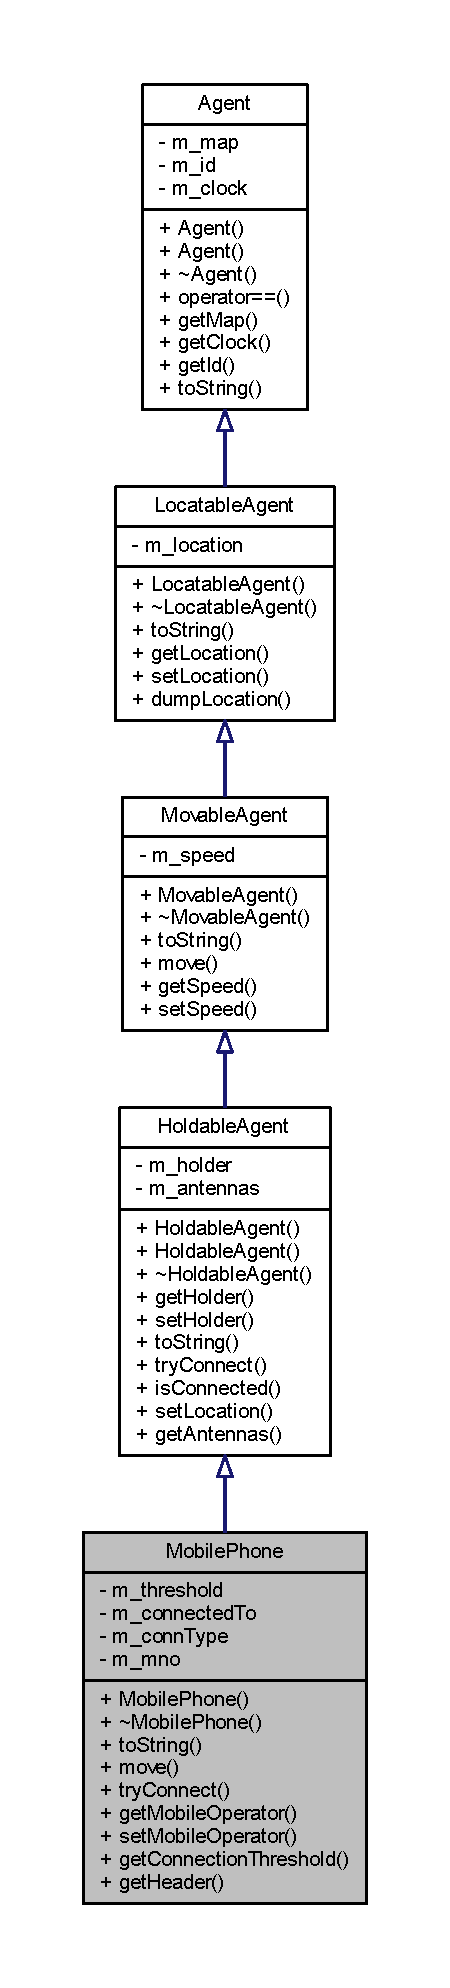
\includegraphics[height=550pt]{class_mobile_phone__inherit__graph}
\end{center}
\end{figure}


Collaboration diagram for Mobile\+Phone\+:
\nopagebreak
\begin{figure}[H]
\begin{center}
\leavevmode
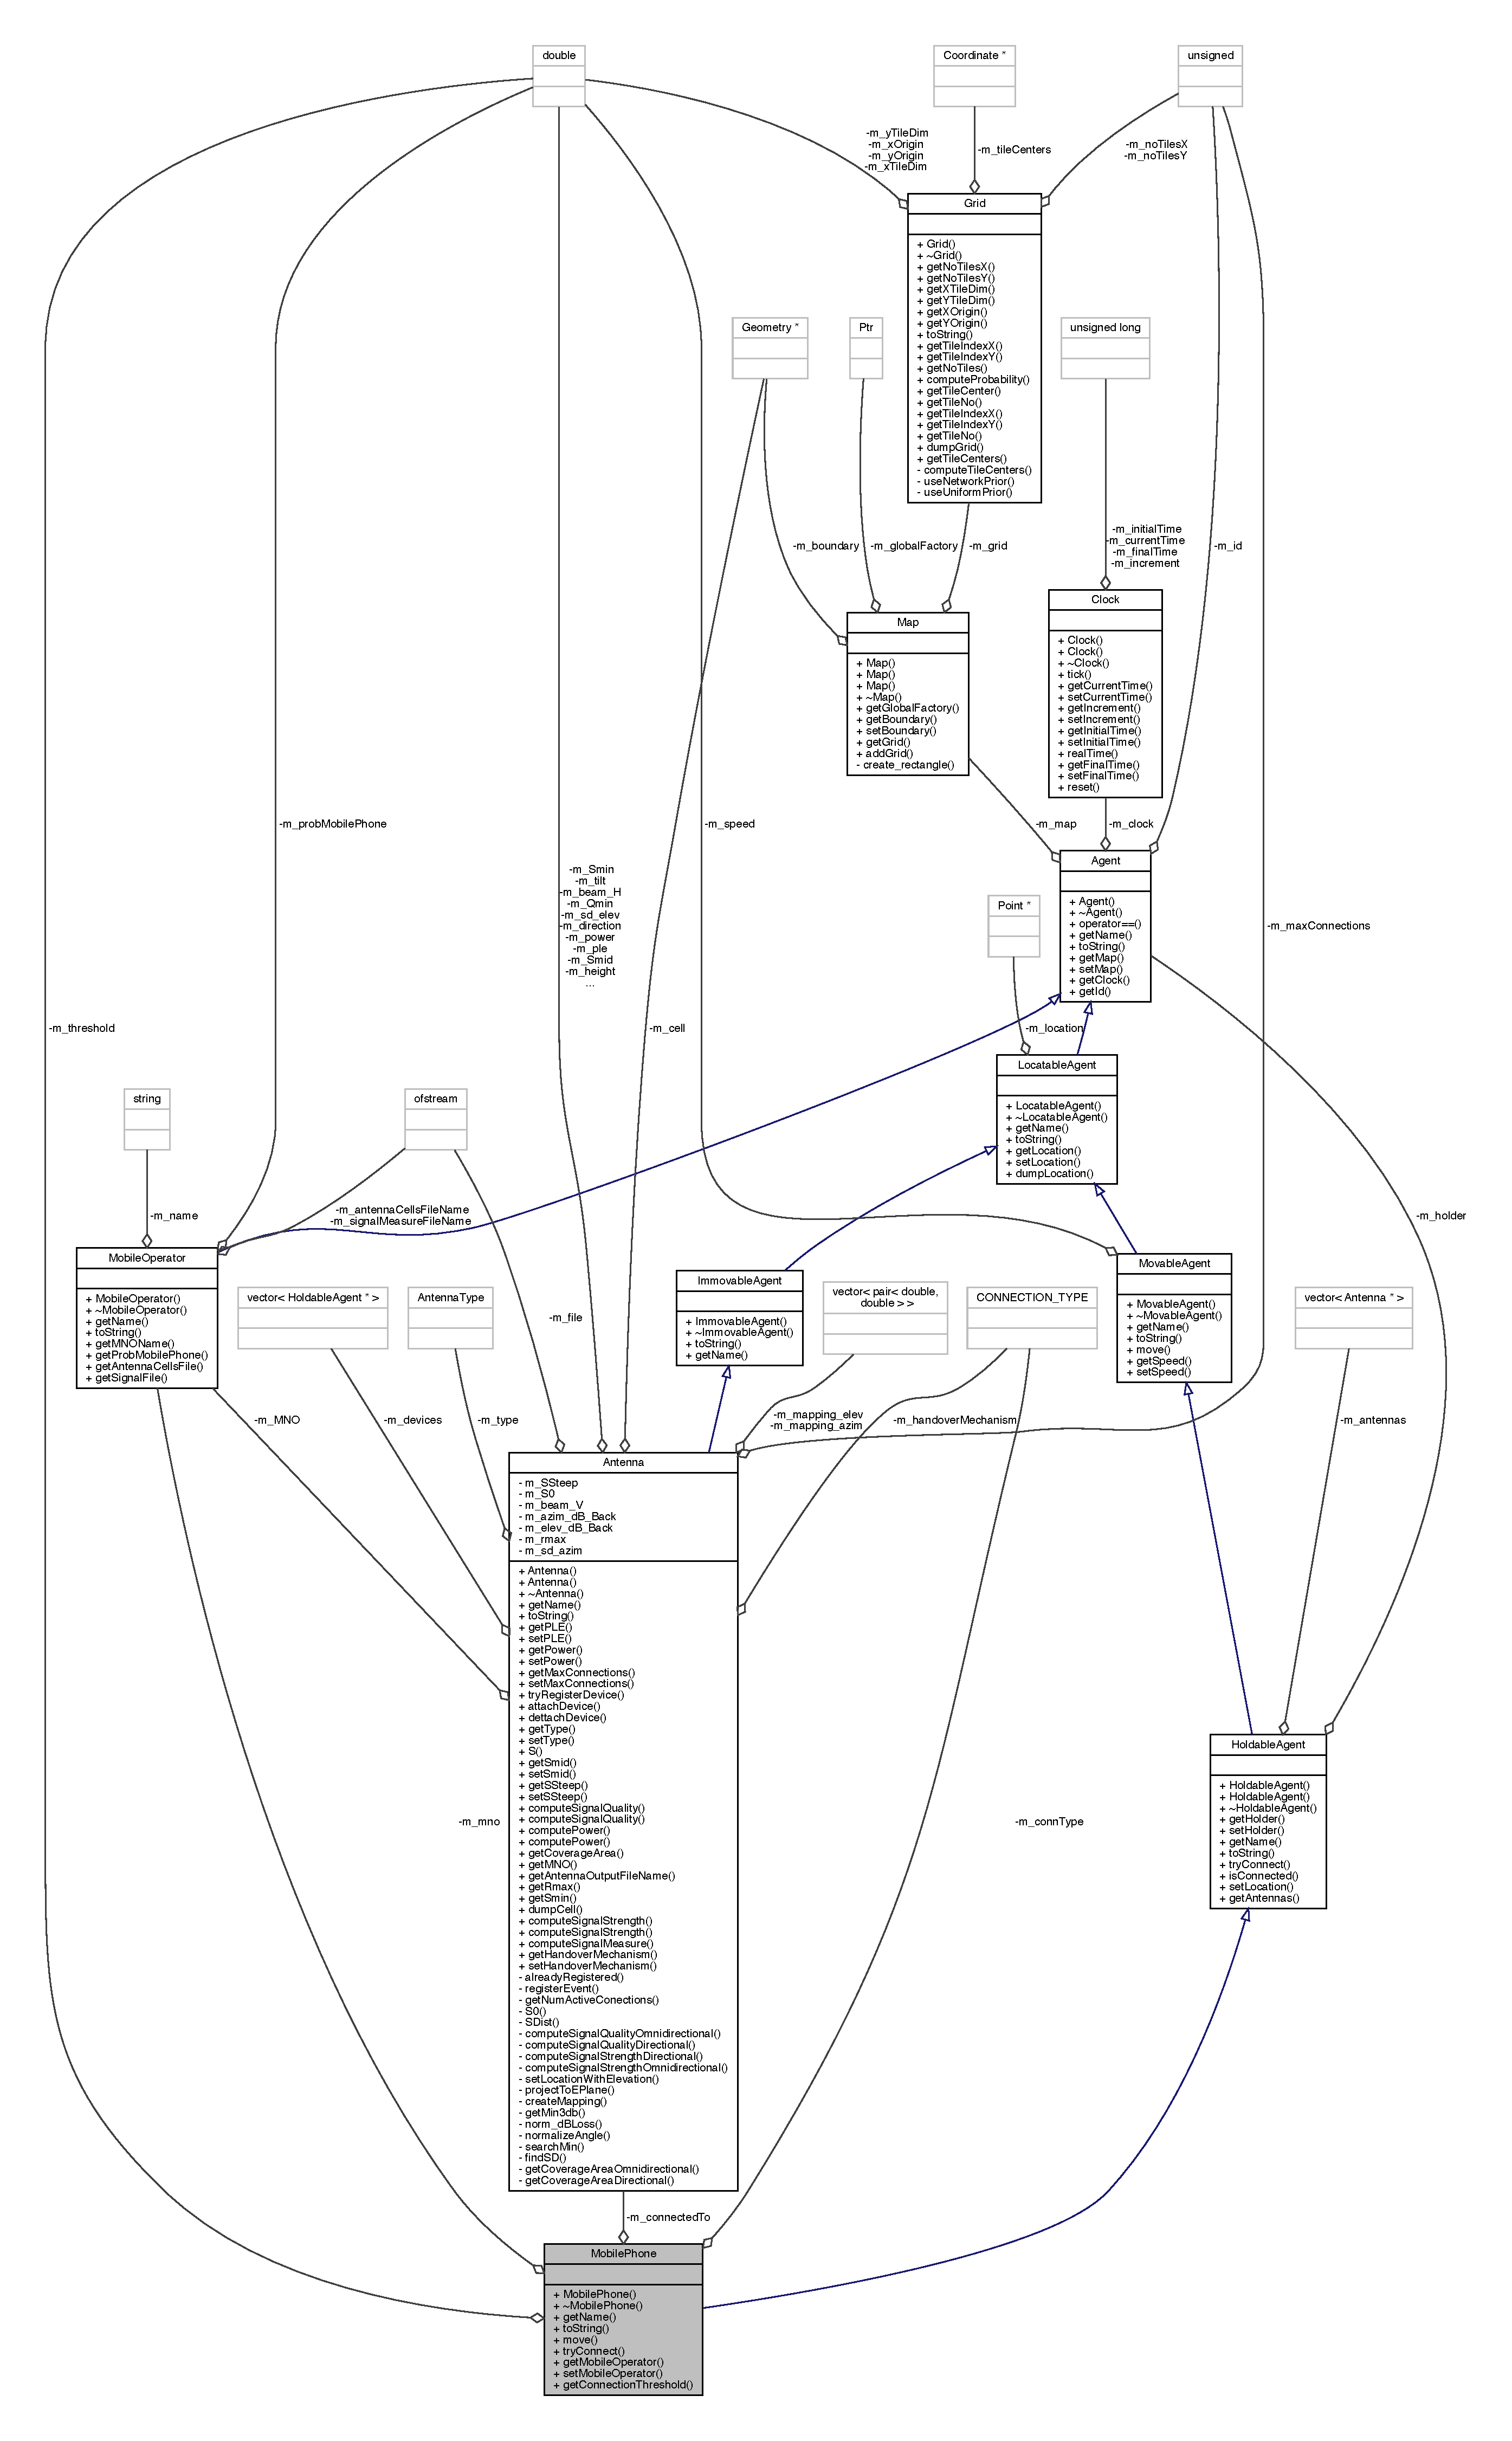
\includegraphics[height=550pt]{class_mobile_phone__coll__graph}
\end{center}
\end{figure}
\subsection*{Public Member Functions}
\begin{DoxyCompactItemize}
\item 
\mbox{\hyperlink{class_mobile_phone_afd7beed70eb2af3baecd9521332ba8eb}{Mobile\+Phone}} (const \mbox{\hyperlink{class_map}{Map}} $\ast$m, const unsigned long id, Point $\ast$init\+Position, \mbox{\hyperlink{class_agent}{Agent}} $\ast$holder, const \mbox{\hyperlink{class_clock}{Clock}} $\ast$clock, double threshold, \mbox{\hyperlink{class_holdable_agent_ae2c334b004d7b9c5a999cf2618e4e518}{Holdable\+Agent\+::\+C\+O\+N\+N\+E\+C\+T\+I\+O\+N\+\_\+\+T\+Y\+PE}} conn\+Type)
\item 
virtual \mbox{\hyperlink{class_mobile_phone_a51db1d9b4fcc52ea9f8d613dae4f6a4b}{$\sim$\+Mobile\+Phone}} ()
\item 
const string \mbox{\hyperlink{class_mobile_phone_a1eeac3141baafa75ebcf26fc3a0e4068}{get\+Name}} () const override
\item 
const string \mbox{\hyperlink{class_mobile_phone_a2b7e556d12a43e380786ad0eccf3ce04}{to\+String}} () const override
\item 
Point $\ast$ \mbox{\hyperlink{class_mobile_phone_a92d77fa5810ddb9c4c482d9c9baea456}{move}} (\mbox{\hyperlink{_movement_type_8h_a8a93b61bc797a7d1907f42796a252493}{Movement\+Type}} mv\+Type) override
\item 
bool \mbox{\hyperlink{class_mobile_phone_ad91afa811cea8ee124167f5941bcda1b}{try\+Connect}} () override
\item 
const \mbox{\hyperlink{class_mobile_operator}{Mobile\+Operator}} $\ast$ \mbox{\hyperlink{class_mobile_phone_aba72025d08c382d8533e0cbb9166999b}{get\+Mobile\+Operator}} () const
\item 
void \mbox{\hyperlink{class_mobile_phone_ad4db8203e8f2e974733357d7c3e6cf28}{set\+Mobile\+Operator}} (\mbox{\hyperlink{class_mobile_operator}{Mobile\+Operator}} $\ast$mno)
\item 
double \mbox{\hyperlink{class_mobile_phone_a57475711a8f85086f50067d219f1181d}{get\+Connection\+Threshold}} () const
\end{DoxyCompactItemize}
\subsection*{Private Attributes}
\begin{DoxyCompactItemize}
\item 
double \mbox{\hyperlink{class_mobile_phone_afb6364675f7cf6e09856f49ae6c10563}{m\+\_\+threshold}}
\item 
\mbox{\hyperlink{class_antenna}{Antenna}} $\ast$ \mbox{\hyperlink{class_mobile_phone_aa143b94346485788c3563228f6043721}{m\+\_\+connected\+To}}
\item 
\mbox{\hyperlink{class_holdable_agent_ae2c334b004d7b9c5a999cf2618e4e518}{Holdable\+Agent\+::\+C\+O\+N\+N\+E\+C\+T\+I\+O\+N\+\_\+\+T\+Y\+PE}} \mbox{\hyperlink{class_mobile_phone_a39f69fef45f380e3922dfe78b904372d}{m\+\_\+conn\+Type}}
\item 
\mbox{\hyperlink{class_mobile_operator}{Mobile\+Operator}} $\ast$ \mbox{\hyperlink{class_mobile_phone_a1b26abc840ac8f8679dd62939330c597}{m\+\_\+mno}}
\end{DoxyCompactItemize}
\subsection*{Additional Inherited Members}


\subsection{Detailed Description}
This class represents a mobile phone. A mobile phone is own by a \mbox{\hyperlink{class_person}{Person}} and it moves on the map together with its owner. While moving, at every time step it tries to connect to an antenna. The connection event is triggered by \mbox{\hyperlink{class_holdable_agent_aec98d2fe325b48d9a84ad3dad44700e0}{set\+Location()}}. The connection to antenna is determined by the signal emitted by antennas. A parameter in the simulation configuration file set the criterion used to connect\+: the power of the signal, the signal strength or the signal quality. 

\subsection{Constructor \& Destructor Documentation}
\mbox{\Hypertarget{class_mobile_phone_afd7beed70eb2af3baecd9521332ba8eb}\label{class_mobile_phone_afd7beed70eb2af3baecd9521332ba8eb}} 
\index{MobilePhone@{MobilePhone}!MobilePhone@{MobilePhone}}
\index{MobilePhone@{MobilePhone}!MobilePhone@{MobilePhone}}
\subsubsection{\texorpdfstring{MobilePhone()}{MobilePhone()}}
{\footnotesize\ttfamily Mobile\+Phone\+::\+Mobile\+Phone (\begin{DoxyParamCaption}\item[{const \mbox{\hyperlink{class_map}{Map}} $\ast$}]{m,  }\item[{const unsigned long}]{id,  }\item[{Point $\ast$}]{init\+Position,  }\item[{\mbox{\hyperlink{class_agent}{Agent}} $\ast$}]{holder,  }\item[{const \mbox{\hyperlink{class_clock}{Clock}} $\ast$}]{clock,  }\item[{double}]{threshold,  }\item[{\mbox{\hyperlink{class_holdable_agent_ae2c334b004d7b9c5a999cf2618e4e518}{Holdable\+Agent\+::\+C\+O\+N\+N\+E\+C\+T\+I\+O\+N\+\_\+\+T\+Y\+PE}}}]{conn\+Type }\end{DoxyParamCaption})\hspace{0.3cm}{\ttfamily [explicit]}}

Builds a new Mobilew\+Phone object with the parameters provided by the user. 
\begin{DoxyParams}{Parameters}
{\em m} & a pointer to the \mbox{\hyperlink{class_map}{Map}} object where the simulation takes place. \\
\hline
{\em id} & the id of the mobile phone. \\
\hline
{\em init\+Position} & the initial location of the phone on the map. \\
\hline
{\em holder} & a pointer to the \mbox{\hyperlink{class_agent}{Agent}} object that owns this mobile phone. \\
\hline
{\em clock} & a pointer to the \mbox{\hyperlink{class_clock}{Clock}} object used in this simulation. \\
\hline
{\em threshold} & the minimum power, signal qaulity or signal strength of the field below which the mobile phone cannot connect to an antenna. \\
\hline
{\em conn\+Type} & the criterion used for the connection to an antenna\+: based on the power of the signal or based on the signal quality. It could take three values\+: Holdable\+Agent\+::\+C\+O\+N\+N\+E\+C\+T\+I\+O\+N\+\_\+\+T\+Y\+P\+E\+::\+U\+S\+I\+N\+G\+\_\+\+P\+O\+W\+ER, Holdable\+Agent\+::\+C\+O\+N\+N\+E\+C\+T\+I\+O\+N\+\_\+\+T\+Y\+P\+E\+::\+U\+S\+I\+N\+G\+\_\+\+S\+I\+G\+N\+A\+L\+\_\+\+Q\+U\+A\+L\+I\+TY or Holdable\+Agent\+::\+C\+O\+N\+N\+E\+C\+T\+I\+O\+N\+\_\+\+T\+Y\+P\+E\+::\+U\+S\+I\+N\+G\+\_\+\+S\+I\+G\+N\+A\+L\+\_\+\+S\+T\+R\+E\+N\+G\+TH. \\
\hline
\end{DoxyParams}
\mbox{\Hypertarget{class_mobile_phone_a51db1d9b4fcc52ea9f8d613dae4f6a4b}\label{class_mobile_phone_a51db1d9b4fcc52ea9f8d613dae4f6a4b}} 
\index{MobilePhone@{MobilePhone}!````~MobilePhone@{$\sim$MobilePhone}}
\index{````~MobilePhone@{$\sim$MobilePhone}!MobilePhone@{MobilePhone}}
\subsubsection{\texorpdfstring{$\sim$MobilePhone()}{~MobilePhone()}}
{\footnotesize\ttfamily virtual Mobile\+Phone\+::$\sim$\+Mobile\+Phone (\begin{DoxyParamCaption}{ }\end{DoxyParamCaption})\hspace{0.3cm}{\ttfamily [virtual]}}

The default destructor. 

\subsection{Member Function Documentation}
\mbox{\Hypertarget{class_mobile_phone_a57475711a8f85086f50067d219f1181d}\label{class_mobile_phone_a57475711a8f85086f50067d219f1181d}} 
\index{MobilePhone@{MobilePhone}!getConnectionThreshold@{getConnectionThreshold}}
\index{getConnectionThreshold@{getConnectionThreshold}!MobilePhone@{MobilePhone}}
\subsubsection{\texorpdfstring{getConnectionThreshold()}{getConnectionThreshold()}}
{\footnotesize\ttfamily double Mobile\+Phone\+::get\+Connection\+Threshold (\begin{DoxyParamCaption}{ }\end{DoxyParamCaption}) const}

Returns the minimum value of the signal strength/power/quality below which the phone cannot use the signal (i.\+e. the signal is considered noise). The returned value is interpreted as signal strength, power or quality according to the connection type. \begin{DoxyReturn}{Returns}
the minimum value of the signal strength/power/quality below which the phone cannot use the signal (i.\+e. the signal is considered noise). 
\end{DoxyReturn}
\mbox{\Hypertarget{class_mobile_phone_aba72025d08c382d8533e0cbb9166999b}\label{class_mobile_phone_aba72025d08c382d8533e0cbb9166999b}} 
\index{MobilePhone@{MobilePhone}!getMobileOperator@{getMobileOperator}}
\index{getMobileOperator@{getMobileOperator}!MobilePhone@{MobilePhone}}
\subsubsection{\texorpdfstring{getMobileOperator()}{getMobileOperator()}}
{\footnotesize\ttfamily const \mbox{\hyperlink{class_mobile_operator}{Mobile\+Operator}}$\ast$ Mobile\+Phone\+::get\+Mobile\+Operator (\begin{DoxyParamCaption}{ }\end{DoxyParamCaption}) const}

Returns the \mbox{\hyperlink{class_mobile_operator}{Mobile\+Operator}} object of this mobile phone. Each \mbox{\hyperlink{class_mobile_phone}{Mobile\+Phone}} should belong to a Mobile Operator. \begin{DoxyReturn}{Returns}
the \mbox{\hyperlink{class_mobile_operator}{Mobile\+Operator}} object of this mobile phone. Each \mbox{\hyperlink{class_mobile_phone}{Mobile\+Phone}} should belong to a Mobile Operator. 
\end{DoxyReturn}
\mbox{\Hypertarget{class_mobile_phone_a1eeac3141baafa75ebcf26fc3a0e4068}\label{class_mobile_phone_a1eeac3141baafa75ebcf26fc3a0e4068}} 
\index{MobilePhone@{MobilePhone}!getName@{getName}}
\index{getName@{getName}!MobilePhone@{MobilePhone}}
\subsubsection{\texorpdfstring{getName()}{getName()}}
{\footnotesize\ttfamily const string Mobile\+Phone\+::get\+Name (\begin{DoxyParamCaption}{ }\end{DoxyParamCaption}) const\hspace{0.3cm}{\ttfamily [override]}, {\ttfamily [virtual]}}

Returns the name of this class. \begin{DoxyReturn}{Returns}
the name of this class. 
\end{DoxyReturn}


Reimplemented from \mbox{\hyperlink{class_holdable_agent_ab330bb40de51a957ef8826af629f94a2}{Holdable\+Agent}}.

\mbox{\Hypertarget{class_mobile_phone_a92d77fa5810ddb9c4c482d9c9baea456}\label{class_mobile_phone_a92d77fa5810ddb9c4c482d9c9baea456}} 
\index{MobilePhone@{MobilePhone}!move@{move}}
\index{move@{move}!MobilePhone@{MobilePhone}}
\subsubsection{\texorpdfstring{move()}{move()}}
{\footnotesize\ttfamily Point$\ast$ Mobile\+Phone\+::move (\begin{DoxyParamCaption}\item[{\mbox{\hyperlink{_movement_type_8h_a8a93b61bc797a7d1907f42796a252493}{Movement\+Type}}}]{mv\+Type }\end{DoxyParamCaption})\hspace{0.3cm}{\ttfamily [inline]}, {\ttfamily [override]}, {\ttfamily [virtual]}}

Makes a step on the map according to an algorithm. The direction and the length of the step is determined by the mv\+Type parameter and by the \mbox{\hyperlink{class_person}{Person}} object who owns this phone. 
\begin{DoxyParams}{Parameters}
{\em mv\+Type} & selects the way people and their phones are moving on the map. At this moment only R\+A\+N\+D\+O\+M\+\_\+\+W\+A\+L\+K\+\_\+\+C\+L\+O\+S\+E\+D\+\_\+\+M\+AP and R\+A\+N\+D\+O\+M\+\_\+\+W\+A\+L\+K\+\_\+\+C\+L\+O\+S\+E\+D\+\_\+\+M\+A\+P\+\_\+\+W\+I\+T\+H\+\_\+\+D\+R\+I\+FT are implemented. R\+A\+N\+D\+O\+M\+\_\+\+W\+A\+L\+K\+\_\+\+C\+L\+O\+S\+E\+D\+\_\+\+M\+AP means that at each time instant the direction is generated as a uniformly distributed random value and the step length is computed multiplying the speed with the time interval set in the simulation configuration file. If a step projects it outside the map, it stops on the boundary. \mbox{\hyperlink{_movement_type_8h_a8a93b61bc797a7d1907f42796a252493a19d5a14b0e46bf765f243b7e2b7b8810}{Movement\+Type\+::\+R\+A\+N\+D\+O\+M\+\_\+\+W\+A\+L\+K\+\_\+\+C\+L\+O\+S\+E\+D\+\_\+\+M\+A\+P\+\_\+\+W\+I\+T\+H\+\_\+\+D\+R\+I\+FT}} means that there is a preference in the direction of the movement. There are two constants defined, S\+I\+M\+\_\+\+T\+R\+E\+N\+D\+\_\+\+A\+N\+G\+L\+E\+\_\+1 and S\+I\+M\+\_\+\+T\+R\+E\+N\+D\+\_\+\+A\+N\+G\+L\+E\+\_\+2 (3P\+I/4 and 5P\+I/4), and in the first half of the simulation the direction is generated as a normal distributed random value with the mean equals to S\+I\+M\+\_\+\+T\+R\+E\+N\+D\+\_\+\+A\+N\+G\+L\+E\+\_\+1 and sd = 0.\+1 while during the second half of the simulation it is generated as a normal distributed random value with the mean equals to S\+I\+M\+\_\+\+T\+R\+E\+N\+D\+\_\+\+A\+N\+G\+L\+E\+\_\+2 and the same sd. Again, a \mbox{\hyperlink{class_movable_agent}{Movable\+Agent}} can only move inside the map boundary. If a step projects it outside the map, it stops on the boundary.\\
\hline
\end{DoxyParams}
\begin{DoxyReturn}{Returns}
the final location after the movement. 
\end{DoxyReturn}


Implements \mbox{\hyperlink{class_movable_agent_a35299e133c6787689b553d74ce5f98f0}{Movable\+Agent}}.

\mbox{\Hypertarget{class_mobile_phone_ad4db8203e8f2e974733357d7c3e6cf28}\label{class_mobile_phone_ad4db8203e8f2e974733357d7c3e6cf28}} 
\index{MobilePhone@{MobilePhone}!setMobileOperator@{setMobileOperator}}
\index{setMobileOperator@{setMobileOperator}!MobilePhone@{MobilePhone}}
\subsubsection{\texorpdfstring{setMobileOperator()}{setMobileOperator()}}
{\footnotesize\ttfamily void Mobile\+Phone\+::set\+Mobile\+Operator (\begin{DoxyParamCaption}\item[{\mbox{\hyperlink{class_mobile_operator}{Mobile\+Operator}} $\ast$}]{mno }\end{DoxyParamCaption})}

Sets the \mbox{\hyperlink{class_mobile_operator}{Mobile\+Operator}} object which owns this phone. 
\begin{DoxyParams}{Parameters}
{\em mno} & the \mbox{\hyperlink{class_mobile_operator}{Mobile\+Operator}} object which owns this phone. \\
\hline
\end{DoxyParams}
\mbox{\Hypertarget{class_mobile_phone_a2b7e556d12a43e380786ad0eccf3ce04}\label{class_mobile_phone_a2b7e556d12a43e380786ad0eccf3ce04}} 
\index{MobilePhone@{MobilePhone}!toString@{toString}}
\index{toString@{toString}!MobilePhone@{MobilePhone}}
\subsubsection{\texorpdfstring{toString()}{toString()}}
{\footnotesize\ttfamily const string Mobile\+Phone\+::to\+String (\begin{DoxyParamCaption}{ }\end{DoxyParamCaption}) const\hspace{0.3cm}{\ttfamily [override]}, {\ttfamily [virtual]}}

Returns a human readable string representation of this class useful to output it to a file or console. \begin{DoxyReturn}{Returns}
a human readable string representation of this class. 
\end{DoxyReturn}


Reimplemented from \mbox{\hyperlink{class_holdable_agent_a2c581226b8994f24b6b2306ae17dbb52}{Holdable\+Agent}}.

\mbox{\Hypertarget{class_mobile_phone_ad91afa811cea8ee124167f5941bcda1b}\label{class_mobile_phone_ad91afa811cea8ee124167f5941bcda1b}} 
\index{MobilePhone@{MobilePhone}!tryConnect@{tryConnect}}
\index{tryConnect@{tryConnect}!MobilePhone@{MobilePhone}}
\subsubsection{\texorpdfstring{tryConnect()}{tryConnect()}}
{\footnotesize\ttfamily bool Mobile\+Phone\+::try\+Connect (\begin{DoxyParamCaption}{ }\end{DoxyParamCaption})\hspace{0.3cm}{\ttfamily [override]}, {\ttfamily [virtual]}}

This method is called after the phone moves (together with its owner) to a new location. It tries to connect the mobile phone to an antenna. The connection method is determined by inspecting the m\+\_\+conn\+Type\+: using the power of the signal, using the quality of the signal or using the signal strength. The value of the m\+\_\+conn\+Type is set by the constructor of the class. If the connection is successfully a pointer to the \mbox{\hyperlink{class_antenna}{Antenna}} object where this mobile phone was connected is stored internally. \begin{DoxyReturn}{Returns}
true if the connection succeeds, false otherwise. 
\end{DoxyReturn}


Implements \mbox{\hyperlink{class_holdable_agent_a0789d757d81b43ee016e9362046f6dea}{Holdable\+Agent}}.



\subsection{Member Data Documentation}
\mbox{\Hypertarget{class_mobile_phone_aa143b94346485788c3563228f6043721}\label{class_mobile_phone_aa143b94346485788c3563228f6043721}} 
\index{MobilePhone@{MobilePhone}!m\_connectedTo@{m\_connectedTo}}
\index{m\_connectedTo@{m\_connectedTo}!MobilePhone@{MobilePhone}}
\subsubsection{\texorpdfstring{m\_connectedTo}{m\_connectedTo}}
{\footnotesize\ttfamily \mbox{\hyperlink{class_antenna}{Antenna}}$\ast$ Mobile\+Phone\+::m\+\_\+connected\+To\hspace{0.3cm}{\ttfamily [private]}}

\mbox{\Hypertarget{class_mobile_phone_a39f69fef45f380e3922dfe78b904372d}\label{class_mobile_phone_a39f69fef45f380e3922dfe78b904372d}} 
\index{MobilePhone@{MobilePhone}!m\_connType@{m\_connType}}
\index{m\_connType@{m\_connType}!MobilePhone@{MobilePhone}}
\subsubsection{\texorpdfstring{m\_connType}{m\_connType}}
{\footnotesize\ttfamily \mbox{\hyperlink{class_holdable_agent_ae2c334b004d7b9c5a999cf2618e4e518}{Holdable\+Agent\+::\+C\+O\+N\+N\+E\+C\+T\+I\+O\+N\+\_\+\+T\+Y\+PE}} Mobile\+Phone\+::m\+\_\+conn\+Type\hspace{0.3cm}{\ttfamily [private]}}

\mbox{\Hypertarget{class_mobile_phone_a1b26abc840ac8f8679dd62939330c597}\label{class_mobile_phone_a1b26abc840ac8f8679dd62939330c597}} 
\index{MobilePhone@{MobilePhone}!m\_mno@{m\_mno}}
\index{m\_mno@{m\_mno}!MobilePhone@{MobilePhone}}
\subsubsection{\texorpdfstring{m\_mno}{m\_mno}}
{\footnotesize\ttfamily \mbox{\hyperlink{class_mobile_operator}{Mobile\+Operator}}$\ast$ Mobile\+Phone\+::m\+\_\+mno\hspace{0.3cm}{\ttfamily [private]}}

\mbox{\Hypertarget{class_mobile_phone_afb6364675f7cf6e09856f49ae6c10563}\label{class_mobile_phone_afb6364675f7cf6e09856f49ae6c10563}} 
\index{MobilePhone@{MobilePhone}!m\_threshold@{m\_threshold}}
\index{m\_threshold@{m\_threshold}!MobilePhone@{MobilePhone}}
\subsubsection{\texorpdfstring{m\_threshold}{m\_threshold}}
{\footnotesize\ttfamily double Mobile\+Phone\+::m\+\_\+threshold\hspace{0.3cm}{\ttfamily [private]}}



The documentation for this class was generated from the following file\+:\begin{DoxyCompactItemize}
\item 
include/\mbox{\hyperlink{_mobile_phone_8h}{Mobile\+Phone.\+h}}\end{DoxyCompactItemize}

\section{Movable\+Agent Class Reference}
\label{class_movable_agent}\index{MovableAgent@{MovableAgent}}


{\ttfamily \#include $<$Movable\+Agent.\+h$>$}

Inheritance diagram for Movable\+Agent\+:\begin{figure}[H]
\begin{center}
\leavevmode
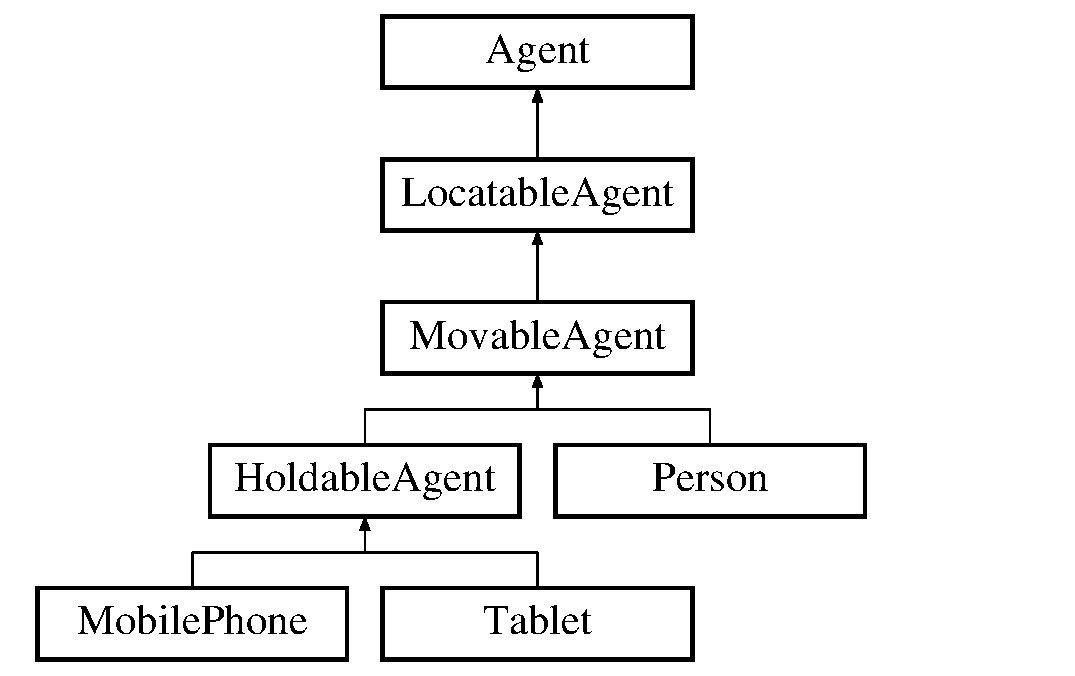
\includegraphics[height=5.000000cm]{class_movable_agent}
\end{center}
\end{figure}
\subsection*{Public Member Functions}
\begin{DoxyCompactItemize}
\item 
\textbf{ Movable\+Agent} (const \textbf{ Map} $\ast$m, const unsigned long id, Point $\ast$init\+Position, const \textbf{ Clock} $\ast$clock, double init\+Speed)
\item 
virtual \textbf{ $\sim$\+Movable\+Agent} ()
\item 
const string \textbf{ get\+Name} () const override
\item 
const string \textbf{ to\+String} () const override
\item 
virtual Point $\ast$ \textbf{ move} (\textbf{ Movement\+Type} type)=0
\item 
double \textbf{ get\+Speed} () const
\item 
void \textbf{ set\+Speed} (double speed)
\end{DoxyCompactItemize}
\subsection*{Private Attributes}
\begin{DoxyCompactItemize}
\item 
double \textbf{ m\+\_\+speed}
\end{DoxyCompactItemize}


\subsection{Detailed Description}
This class represents an agent that can move inside the map 

Definition at line 25 of file Movable\+Agent.\+h.



\subsection{Constructor \& Destructor Documentation}
\mbox{\label{class_movable_agent_ad76b14a044181a57ade71f1267a2ccbd}} 
\index{MovableAgent@{MovableAgent}!MovableAgent@{MovableAgent}}
\index{MovableAgent@{MovableAgent}!MovableAgent@{MovableAgent}}
\subsubsection{MovableAgent()}
{\footnotesize\ttfamily Movable\+Agent\+::\+Movable\+Agent (\begin{DoxyParamCaption}\item[{const \textbf{ Map} $\ast$}]{m,  }\item[{const unsigned long}]{id,  }\item[{Point $\ast$}]{init\+Position,  }\item[{const \textbf{ Clock} $\ast$}]{clock,  }\item[{double}]{init\+Speed }\end{DoxyParamCaption})\hspace{0.3cm}{\ttfamily [explicit]}}

Builds a new object with the parameters provided by user 
\begin{DoxyParams}{Parameters}
{\em m} & a pointer to the map used by the simulation \\
\hline
{\em id} & the id of the object \\
\hline
{\em init\+Position} & the initial location on map \\
\hline
{\em clock} & a pointer to the \doxyref{Clock}{p.}{class_clock} object used by this simulation \\
\hline
{\em init\+Speed} & the initial speed of the agent \\
\hline
\end{DoxyParams}
\mbox{\label{class_movable_agent_a20eb9ddcc953137e63e035837918206c}} 
\index{MovableAgent@{MovableAgent}!````~MovableAgent@{$\sim$MovableAgent}}
\index{````~MovableAgent@{$\sim$MovableAgent}!MovableAgent@{MovableAgent}}
\subsubsection{$\sim$MovableAgent()}
{\footnotesize\ttfamily virtual Movable\+Agent\+::$\sim$\+Movable\+Agent (\begin{DoxyParamCaption}{ }\end{DoxyParamCaption})\hspace{0.3cm}{\ttfamily [virtual]}}

Destructor 

\subsection{Member Function Documentation}
\mbox{\label{class_movable_agent_abcc1218876c39c996f2cb1eba2b96379}} 
\index{MovableAgent@{MovableAgent}!getName@{getName}}
\index{getName@{getName}!MovableAgent@{MovableAgent}}
\subsubsection{getName()}
{\footnotesize\ttfamily const string Movable\+Agent\+::get\+Name (\begin{DoxyParamCaption}{ }\end{DoxyParamCaption}) const\hspace{0.3cm}{\ttfamily [override]}, {\ttfamily [virtual]}}

Returns the name of the class \begin{DoxyReturn}{Returns}
the name of the class 
\end{DoxyReturn}


Reimplemented from \textbf{ Locatable\+Agent} \doxyref{}{p.}{class_locatable_agent_a754105958bb672744b525538f1584a7b}.



Reimplemented in \textbf{ Person} \doxyref{}{p.}{class_person_aa2a6f8d7f1d94045a03ca578f2ed272c}, and \textbf{ Tablet} \doxyref{}{p.}{class_tablet_adc7196aaee1e9714236b7cd8825d5826}.

\mbox{\label{class_movable_agent_a12fcdaee60f5bb29f15fe113a7dacaac}} 
\index{MovableAgent@{MovableAgent}!getSpeed@{getSpeed}}
\index{getSpeed@{getSpeed}!MovableAgent@{MovableAgent}}
\subsubsection{getSpeed()}
{\footnotesize\ttfamily double Movable\+Agent\+::get\+Speed (\begin{DoxyParamCaption}{ }\end{DoxyParamCaption}) const}

Returns the speed of this agent \begin{DoxyReturn}{Returns}
the speed of this agent 
\end{DoxyReturn}
\mbox{\label{class_movable_agent_a35299e133c6787689b553d74ce5f98f0}} 
\index{MovableAgent@{MovableAgent}!move@{move}}
\index{move@{move}!MovableAgent@{MovableAgent}}
\subsubsection{move()}
{\footnotesize\ttfamily virtual Point$\ast$ Movable\+Agent\+::move (\begin{DoxyParamCaption}\item[{\textbf{ Movement\+Type}}]{type }\end{DoxyParamCaption})\hspace{0.3cm}{\ttfamily [pure virtual]}}

A pure virtual method that moves the agent to a new location on the map 
\begin{DoxyParams}{Parameters}
{\em type} & the type of the movement. At this moment only \\
\hline
\end{DoxyParams}
\begin{DoxyReturn}{Returns}

\end{DoxyReturn}


Implemented in \textbf{ Person} \doxyref{}{p.}{class_person_a89843e85f14abc08422273c20252ae23}, \textbf{ Mobile\+Phone} \doxyref{}{p.}{class_mobile_phone_a92d77fa5810ddb9c4c482d9c9baea456}, and \textbf{ Tablet} \doxyref{}{p.}{class_tablet_a0021a8d61f496d84540f675b1cb7d080}.

\mbox{\label{class_movable_agent_ae2ef452e81789a4370e7dee32a9cc67e}} 
\index{MovableAgent@{MovableAgent}!setSpeed@{setSpeed}}
\index{setSpeed@{setSpeed}!MovableAgent@{MovableAgent}}
\subsubsection{setSpeed()}
{\footnotesize\ttfamily void Movable\+Agent\+::set\+Speed (\begin{DoxyParamCaption}\item[{double}]{speed }\end{DoxyParamCaption})}

Sets the speed of this agent 
\begin{DoxyParams}{Parameters}
{\em speed} & the speed of this agent \\
\hline
\end{DoxyParams}
\mbox{\label{class_movable_agent_a1dee2a6bf93f01006fadfb6fba6c9a59}} 
\index{MovableAgent@{MovableAgent}!toString@{toString}}
\index{toString@{toString}!MovableAgent@{MovableAgent}}
\subsubsection{toString()}
{\footnotesize\ttfamily const string Movable\+Agent\+::to\+String (\begin{DoxyParamCaption}{ }\end{DoxyParamCaption}) const\hspace{0.3cm}{\ttfamily [override]}, {\ttfamily [virtual]}}

Builds a human readable string representation of the agent \begin{DoxyReturn}{Returns}
a human readable string representation of the agent 
\end{DoxyReturn}


Reimplemented from \textbf{ Locatable\+Agent} \doxyref{}{p.}{class_locatable_agent_a88674f4c8ab9b1b2f3986b226bf4244f}.



Reimplemented in \textbf{ Person} \doxyref{}{p.}{class_person_a68872538da519d0a04297f43376db27c}, and \textbf{ Tablet} \doxyref{}{p.}{class_tablet_a3fae01e7d526699476221c6a686a4fba}.



\subsection{Member Data Documentation}
\mbox{\label{class_movable_agent_ac725b42e7b968740a59c3e1033d69ac5}} 
\index{MovableAgent@{MovableAgent}!m\_speed@{m\_speed}}
\index{m\_speed@{m\_speed}!MovableAgent@{MovableAgent}}
\subsubsection{m\_speed}
{\footnotesize\ttfamily double Movable\+Agent\+::m\+\_\+speed\hspace{0.3cm}{\ttfamily [private]}}



Definition at line 75 of file Movable\+Agent.\+h.



The documentation for this class was generated from the following file\+:\begin{DoxyCompactItemize}
\item 
include/\textbf{ Movable\+Agent.\+h}\end{DoxyCompactItemize}

\hypertarget{class_person}{}\section{Person Class Reference}
\label{class_person}\index{Person@{Person}}


{\ttfamily \#include $<$Person.\+h$>$}



Inheritance diagram for Person\+:
\nopagebreak
\begin{figure}[H]
\begin{center}
\leavevmode
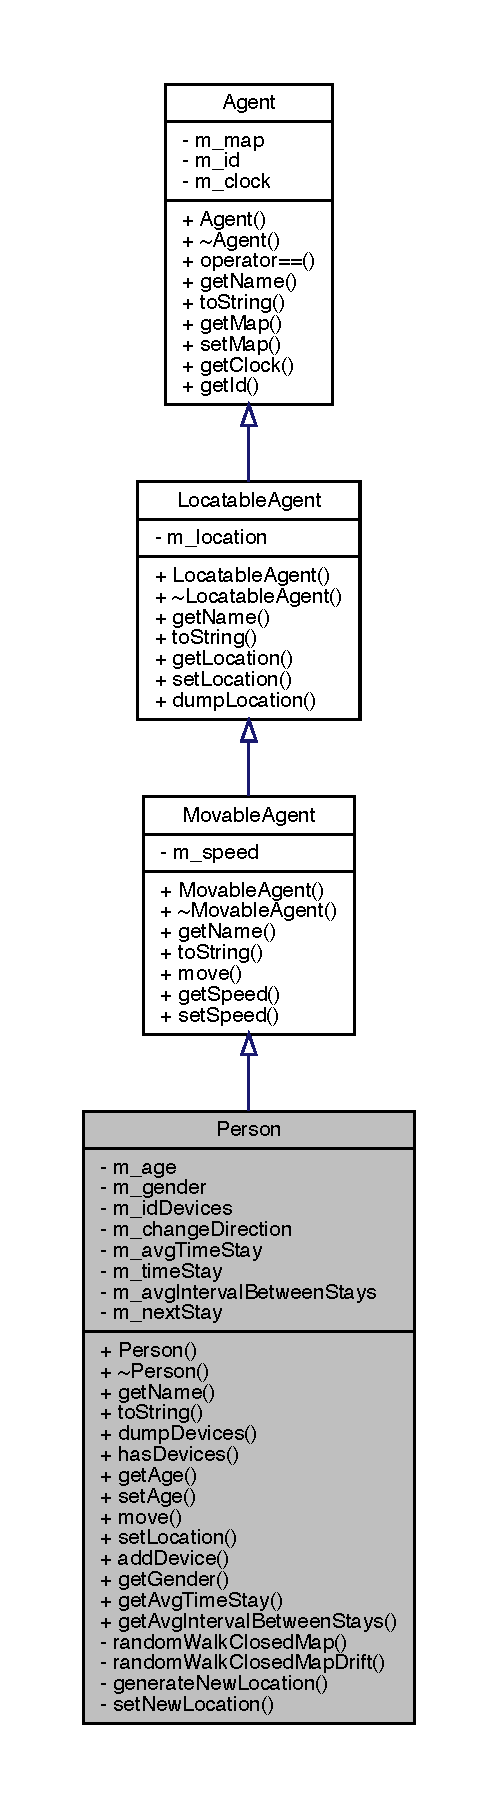
\includegraphics[height=550pt]{class_person__inherit__graph}
\end{center}
\end{figure}


Collaboration diagram for Person\+:
\nopagebreak
\begin{figure}[H]
\begin{center}
\leavevmode
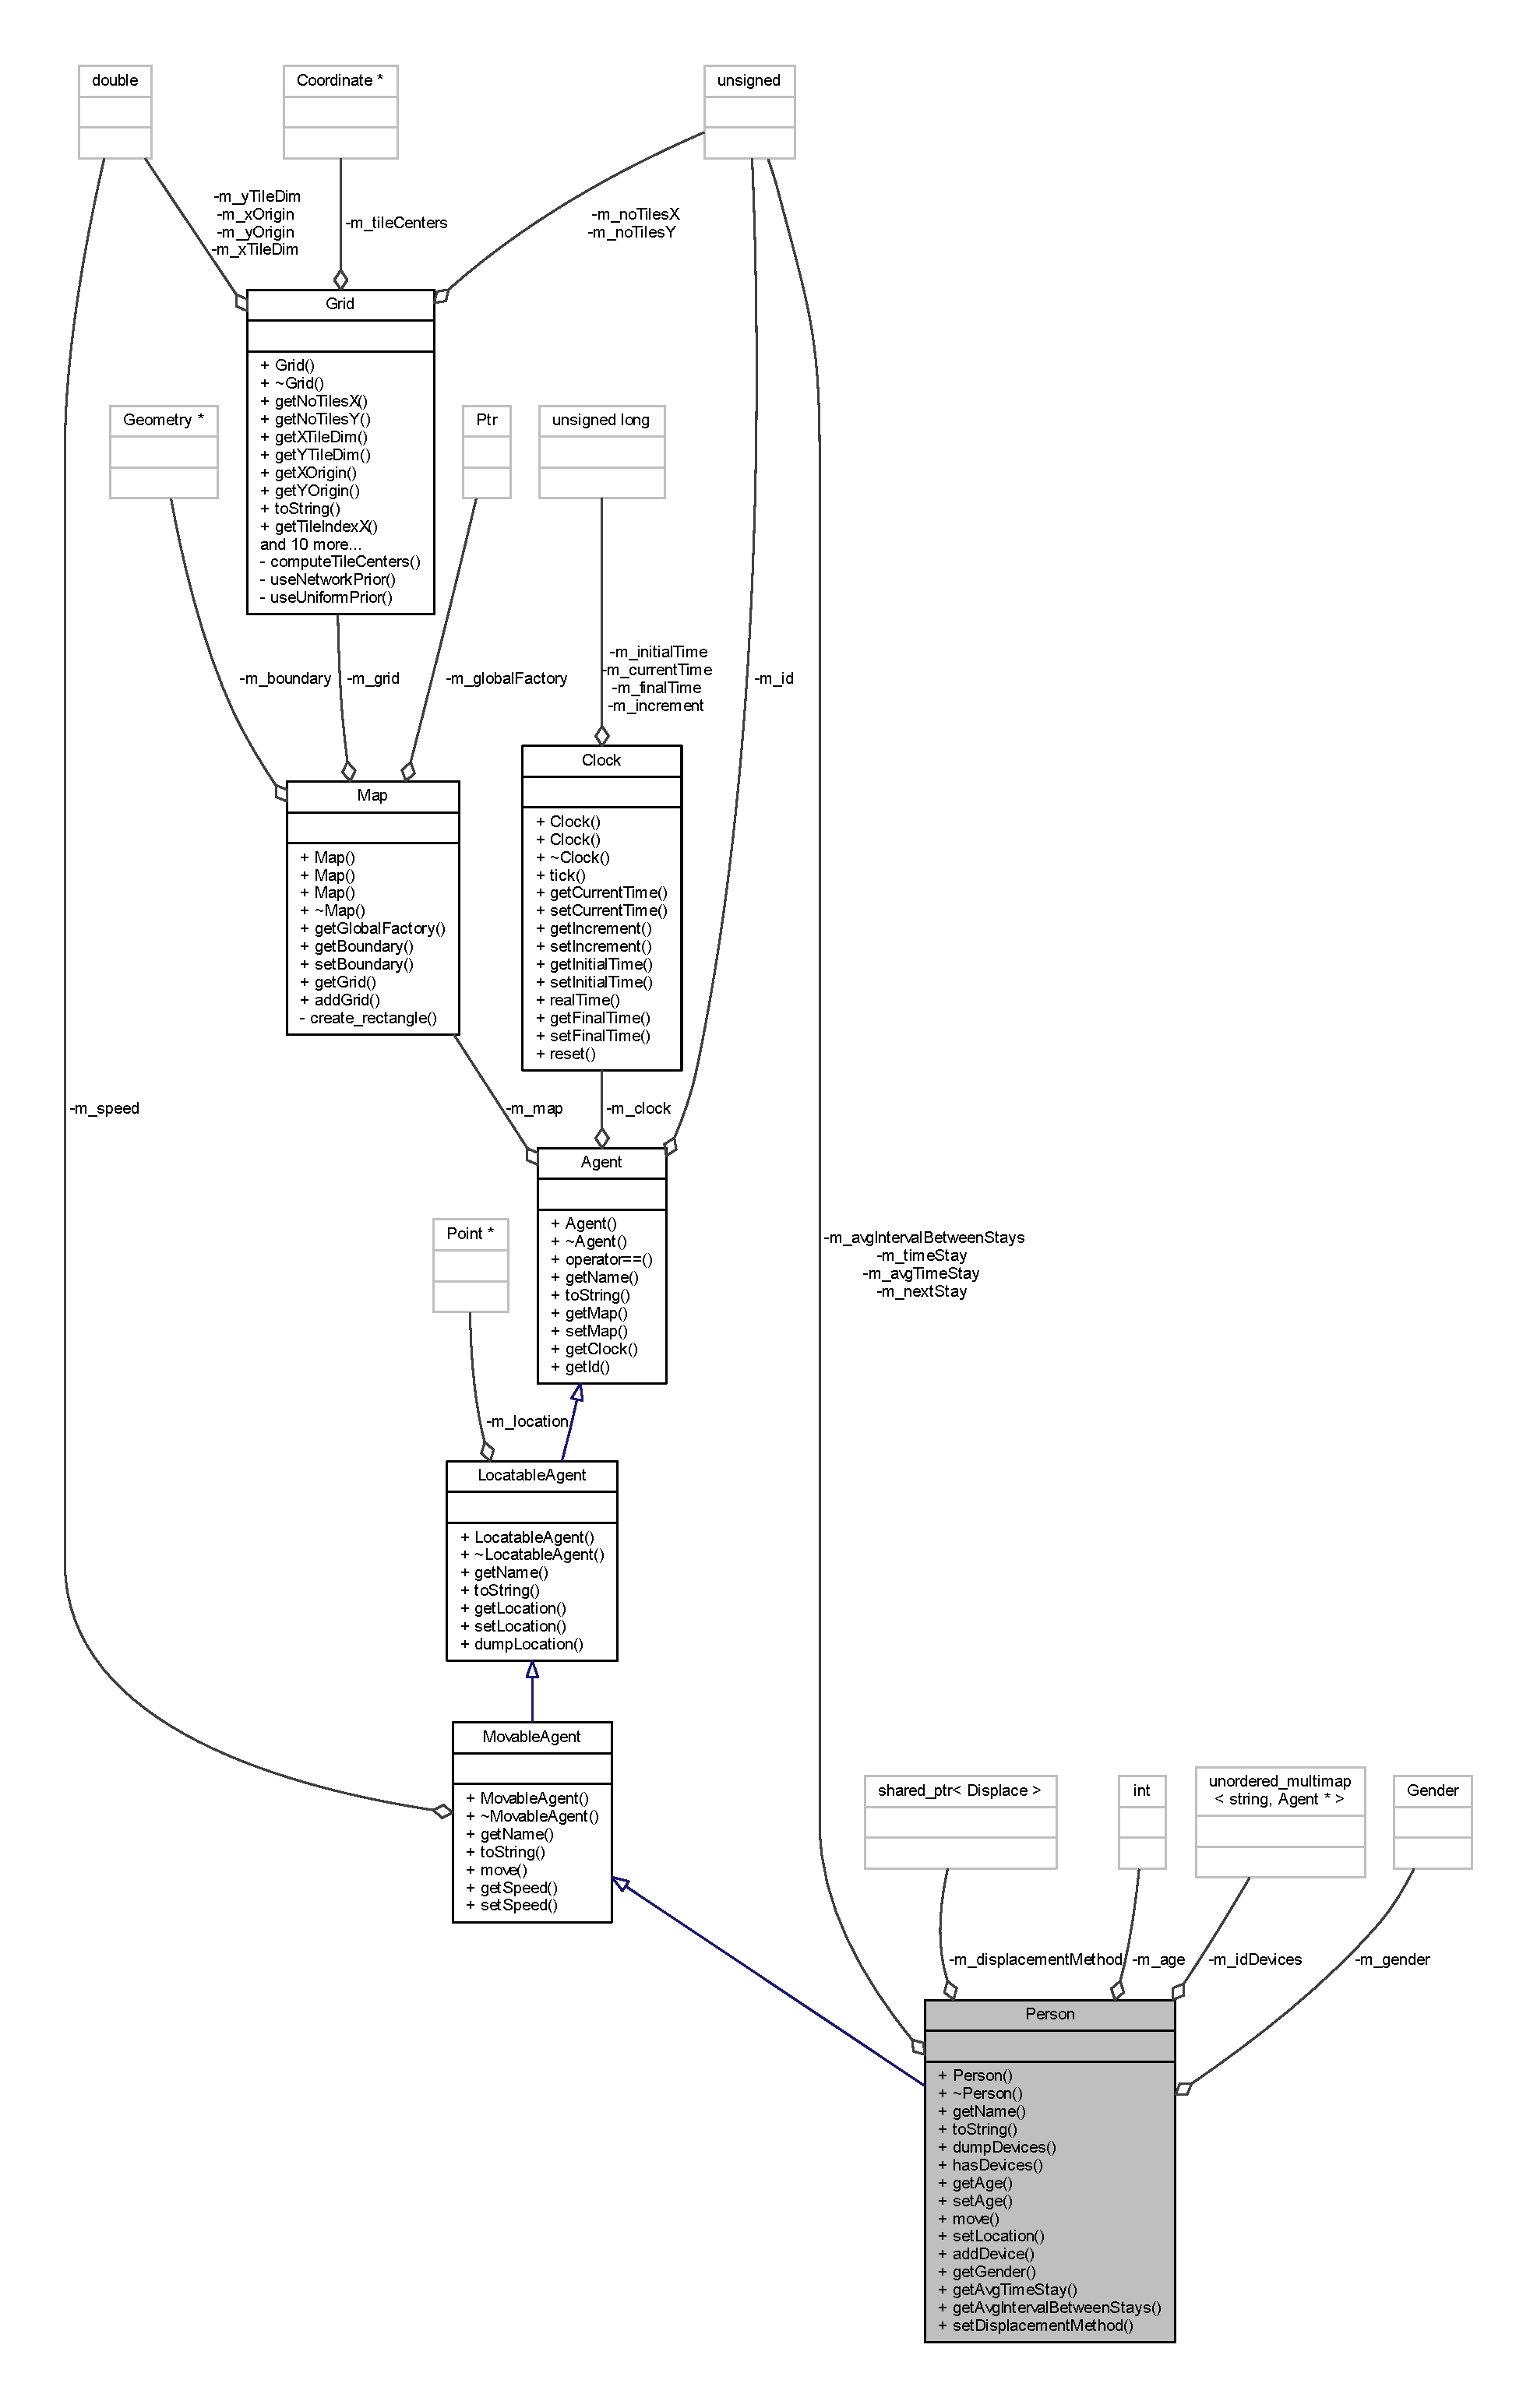
\includegraphics[height=550pt]{class_person__coll__graph}
\end{center}
\end{figure}
\subsection*{Public Types}
\begin{DoxyCompactItemize}
\item 
enum \hyperlink{class_person_aff84ca16bd4dbf364614d86f20b29dd2}{Gender} \{ \hyperlink{class_person_aff84ca16bd4dbf364614d86f20b29dd2a16691f7cc6595f87b71d9b43ad23fcb4}{M\+A\+LE}, 
\hyperlink{class_person_aff84ca16bd4dbf364614d86f20b29dd2a8ee21010fb2d8e8794ef72be368da064}{F\+E\+M\+A\+LE}
 \}
\end{DoxyCompactItemize}
\subsection*{Public Member Functions}
\begin{DoxyCompactItemize}
\item 
\hyperlink{class_person_a1fb64d7ef7c528d01dd09b2099b00e38}{Person} (const \hyperlink{class_map}{Map} $\ast$m, const unsigned long id, Point $\ast$init\+Position, const \hyperlink{class_clock}{Clock} $\ast$clock, double init\+Speed, int age, \hyperlink{class_person_aff84ca16bd4dbf364614d86f20b29dd2}{Gender} gender, unsigned long time\+Stay, unsigned long interval\+Between\+Stays)
\item 
virtual \hyperlink{class_person_a6b5729bb56531c93312b1179c8ee4b71}{$\sim$\+Person} ()
\item 
const string \hyperlink{class_person_a68872538da519d0a04297f43376db27c}{to\+String} () const override
\item 
string \hyperlink{class_person_a0bc06f77b3e8a151f8c5cc77459895c9}{dump\+Devices} ()
\item 
bool \hyperlink{class_person_a40d6f2c716dd3c9794067817a3fb9165}{has\+Devices} ()
\item 
int \hyperlink{class_person_a4b66dbee570398920b8fb6aacddd2559}{get\+Age} () const
\item 
void \hyperlink{class_person_ac8ade54c27a0657c987c395ff04a9d46}{set\+Age} (int age)
\item 
virtual Point $\ast$ \hyperlink{class_person_a922e0462a1e7eac6523a9a864ce27afc}{move} () override
\item 
virtual void \hyperlink{class_person_a05f4ac2107d59e03f0f336eda08aa358}{set\+Location} (Point $\ast$pt) override
\item 
void \hyperlink{class_person_a3ce0a72a98c2e723e48dcd7b4d9af599}{add\+Device} (string type, \hyperlink{class_agent}{Agent} $\ast$agent)
\item 
void \hyperlink{class_person_a89ada26d3541bc82e514dae833dc959d}{set\+Displacement\+Method} (const shared\+\_\+ptr$<$ \hyperlink{class_displace}{Displace} $>$ \&displace)
\end{DoxyCompactItemize}
\subsection*{Static Public Member Functions}
\begin{DoxyCompactItemize}
\item 
static const string \hyperlink{class_person_a6bebe59c354f26f4cb983185d6084181}{get\+Header} ()
\end{DoxyCompactItemize}
\subsection*{Private Attributes}
\begin{DoxyCompactItemize}
\item 
int \hyperlink{class_person_a743e071da10a5ac9150f61df919cfbb4}{m\+\_\+age}
\item 
\hyperlink{class_person_aff84ca16bd4dbf364614d86f20b29dd2}{Gender} \hyperlink{class_person_ade9cdf49acde95c75f19f0b0d24c8c9a}{m\+\_\+gender}
\item 
unordered\+\_\+multimap$<$ string, \hyperlink{class_agent}{Agent} $\ast$ $>$ \hyperlink{class_person_a95b2e60a54b72aea51a7600048e76291}{m\+\_\+id\+Devices}
\item 
unsigned long \hyperlink{class_person_a8c9502459dd59182d11f60f429b44457}{m\+\_\+avg\+Time\+Stay}
\item 
unsigned long \hyperlink{class_person_a5554109f1f3a7c466f02346d0061c6e7}{m\+\_\+time\+Stay}
\item 
unsigned long \hyperlink{class_person_a62a07c9565931a618a09be7510dde07c}{m\+\_\+avg\+Interval\+Between\+Stays}
\item 
unsigned long \hyperlink{class_person_ad8809184fc32b28b1bcc115b10493b55}{m\+\_\+next\+Stay}
\item 
shared\+\_\+ptr$<$ \hyperlink{class_displace}{Displace} $>$ \hyperlink{class_person_a92ceead10a7ca858d2151391e4421843}{m\+\_\+displacement\+Method}
\end{DoxyCompactItemize}


\subsection{Detailed Description}
This class represents a person that can have 0,1 or 2 mobile phone(s). During the simulation the person move around the map, carrying his/her mobile devices. 

\subsection{Member Enumeration Documentation}
\mbox{\Hypertarget{class_person_aff84ca16bd4dbf364614d86f20b29dd2}\label{class_person_aff84ca16bd4dbf364614d86f20b29dd2}} 
\index{Person@{Person}!Gender@{Gender}}
\index{Gender@{Gender}!Person@{Person}}
\subsubsection{\texorpdfstring{Gender}{Gender}}
{\footnotesize\ttfamily enum \hyperlink{class_person_aff84ca16bd4dbf364614d86f20b29dd2}{Person\+::\+Gender}}

\begin{DoxyEnumFields}{Enumerator}
\raisebox{\heightof{T}}[0pt][0pt]{\index{M\+A\+LE@{M\+A\+LE}!Person@{Person}}\index{Person@{Person}!M\+A\+LE@{M\+A\+LE}}}\mbox{\Hypertarget{class_person_aff84ca16bd4dbf364614d86f20b29dd2a16691f7cc6595f87b71d9b43ad23fcb4}\label{class_person_aff84ca16bd4dbf364614d86f20b29dd2a16691f7cc6595f87b71d9b43ad23fcb4}} 
M\+A\+LE&\\
\hline

\raisebox{\heightof{T}}[0pt][0pt]{\index{F\+E\+M\+A\+LE@{F\+E\+M\+A\+LE}!Person@{Person}}\index{Person@{Person}!F\+E\+M\+A\+LE@{F\+E\+M\+A\+LE}}}\mbox{\Hypertarget{class_person_aff84ca16bd4dbf364614d86f20b29dd2a8ee21010fb2d8e8794ef72be368da064}\label{class_person_aff84ca16bd4dbf364614d86f20b29dd2a8ee21010fb2d8e8794ef72be368da064}} 
F\+E\+M\+A\+LE&\\
\hline

\end{DoxyEnumFields}


\subsection{Constructor \& Destructor Documentation}
\mbox{\Hypertarget{class_person_a1fb64d7ef7c528d01dd09b2099b00e38}\label{class_person_a1fb64d7ef7c528d01dd09b2099b00e38}} 
\index{Person@{Person}!Person@{Person}}
\index{Person@{Person}!Person@{Person}}
\subsubsection{\texorpdfstring{Person()}{Person()}}
{\footnotesize\ttfamily Person\+::\+Person (\begin{DoxyParamCaption}\item[{const \hyperlink{class_map}{Map} $\ast$}]{m,  }\item[{const unsigned long}]{id,  }\item[{Point $\ast$}]{init\+Position,  }\item[{const \hyperlink{class_clock}{Clock} $\ast$}]{clock,  }\item[{double}]{init\+Speed,  }\item[{int}]{age,  }\item[{\hyperlink{class_person_aff84ca16bd4dbf364614d86f20b29dd2}{Gender}}]{gender,  }\item[{unsigned long}]{time\+Stay,  }\item[{unsigned long}]{interval\+Between\+Stays }\end{DoxyParamCaption})\hspace{0.3cm}{\ttfamily [explicit]}}

Builds a new \hyperlink{class_person}{Person} object with the characteristics given as parameters. 
\begin{DoxyParams}{Parameters}
{\em m} & a pointer to the \hyperlink{class_map}{Map} object where this \hyperlink{class_person}{Person} move. \\
\hline
{\em id} & the id of the \hyperlink{class_person}{Person}. \\
\hline
{\em init\+Position} & the initial location of the person on the map. \\
\hline
{\em clock} & a pointer to a \hyperlink{class_clock}{Clock} object used for this simulation. \\
\hline
{\em init\+Speed} & the initial speed of this person. It is provided in the configuration file. \\
\hline
{\em age} & the age of the person. The age is generated using a uniform or a normal distribution. \\
\hline
{\em gender} & the gender of the person. \\
\hline
{\em time\+Stay} & the average time of a stop \\
\hline
{\em interval\+Between\+Stays} & the average time between two consecutive stops. \\
\hline
\end{DoxyParams}
\mbox{\Hypertarget{class_person_a6b5729bb56531c93312b1179c8ee4b71}\label{class_person_a6b5729bb56531c93312b1179c8ee4b71}} 
\index{Person@{Person}!````~Person@{$\sim$\+Person}}
\index{````~Person@{$\sim$\+Person}!Person@{Person}}
\subsubsection{\texorpdfstring{$\sim$\+Person()}{~Person()}}
{\footnotesize\ttfamily virtual Person\+::$\sim$\+Person (\begin{DoxyParamCaption}{ }\end{DoxyParamCaption})\hspace{0.3cm}{\ttfamily [virtual]}}

The default destructor. 

\subsection{Member Function Documentation}
\mbox{\Hypertarget{class_person_a3ce0a72a98c2e723e48dcd7b4d9af599}\label{class_person_a3ce0a72a98c2e723e48dcd7b4d9af599}} 
\index{Person@{Person}!add\+Device@{add\+Device}}
\index{add\+Device@{add\+Device}!Person@{Person}}
\subsubsection{\texorpdfstring{add\+Device()}{addDevice()}}
{\footnotesize\ttfamily void Person\+::add\+Device (\begin{DoxyParamCaption}\item[{string}]{type,  }\item[{\hyperlink{class_agent}{Agent} $\ast$}]{agent }\end{DoxyParamCaption})}

Add a mobile device to this person. Internally, all mobile devices are kept in an unordered\+\_\+multimap as pairs $<$name of the device class, pointer to the device object$>$ 
\begin{DoxyParams}{Parameters}
{\em type} & the name of the device\textquotesingle{}s class. \\
\hline
{\em agent} & a pointer to the device object. \\
\hline
\end{DoxyParams}
\mbox{\Hypertarget{class_person_a0bc06f77b3e8a151f8c5cc77459895c9}\label{class_person_a0bc06f77b3e8a151f8c5cc77459895c9}} 
\index{Person@{Person}!dump\+Devices@{dump\+Devices}}
\index{dump\+Devices@{dump\+Devices}!Person@{Person}}
\subsubsection{\texorpdfstring{dump\+Devices()}{dumpDevices()}}
{\footnotesize\ttfamily string Person\+::dump\+Devices (\begin{DoxyParamCaption}{ }\end{DoxyParamCaption})}

Builds a string containing a list with the ids of the mobile devices that this person owns. \begin{DoxyReturn}{Returns}
a string containing a list with the ids of the mobile devices that this person owns. 
\end{DoxyReturn}
\mbox{\Hypertarget{class_person_a4b66dbee570398920b8fb6aacddd2559}\label{class_person_a4b66dbee570398920b8fb6aacddd2559}} 
\index{Person@{Person}!get\+Age@{get\+Age}}
\index{get\+Age@{get\+Age}!Person@{Person}}
\subsubsection{\texorpdfstring{get\+Age()}{getAge()}}
{\footnotesize\ttfamily int Person\+::get\+Age (\begin{DoxyParamCaption}{ }\end{DoxyParamCaption}) const}

Returns the age of the person. \begin{DoxyReturn}{Returns}
the age of the person. 
\end{DoxyReturn}
\mbox{\Hypertarget{class_person_a6bebe59c354f26f4cb983185d6084181}\label{class_person_a6bebe59c354f26f4cb983185d6084181}} 
\index{Person@{Person}!get\+Header@{get\+Header}}
\index{get\+Header@{get\+Header}!Person@{Person}}
\subsubsection{\texorpdfstring{get\+Header()}{getHeader()}}
{\footnotesize\ttfamily static const string Person\+::get\+Header (\begin{DoxyParamCaption}{ }\end{DoxyParamCaption})\hspace{0.3cm}{\ttfamily [static]}}

\mbox{\Hypertarget{class_person_a40d6f2c716dd3c9794067817a3fb9165}\label{class_person_a40d6f2c716dd3c9794067817a3fb9165}} 
\index{Person@{Person}!has\+Devices@{has\+Devices}}
\index{has\+Devices@{has\+Devices}!Person@{Person}}
\subsubsection{\texorpdfstring{has\+Devices()}{hasDevices()}}
{\footnotesize\ttfamily bool Person\+::has\+Devices (\begin{DoxyParamCaption}{ }\end{DoxyParamCaption})}

returns true if this person has at least a mobile device, false otherwise. \begin{DoxyReturn}{Returns}

\end{DoxyReturn}
\mbox{\Hypertarget{class_person_a922e0462a1e7eac6523a9a864ce27afc}\label{class_person_a922e0462a1e7eac6523a9a864ce27afc}} 
\index{Person@{Person}!move@{move}}
\index{move@{move}!Person@{Person}}
\subsubsection{\texorpdfstring{move()}{move()}}
{\footnotesize\ttfamily virtual Point$\ast$ Person\+::move (\begin{DoxyParamCaption}{ }\end{DoxyParamCaption})\hspace{0.3cm}{\ttfamily [override]}, {\ttfamily [virtual]}}

Makes a step on the map according to an algorithm. The direction and the length of the step is determined by the displacement strategy set at the \hyperlink{class_person}{Person} creation moment and currently two strategies are supported\+: \hyperlink{class_random_walk_displacement}{Random\+Walk\+Displacement} and \hyperlink{class_random_walk_drift_displacement}{Random\+Walk\+Drift\+Displacement}. \hyperlink{class_random_walk_displacement}{Random\+Walk\+Displacement} means that at each time instant the direction is generated as a uniformly distributed random value and the step length is computed multiplying the speed with the time interval set in the simulation configuration file. If a step projects it outside the map, it stops on the boundary. \hyperlink{class_random_walk_drift_displacement}{Random\+Walk\+Drift\+Displacement} means that there is a preference in the direction of the movement. There are two constants defined, S\+I\+M\+\_\+\+T\+R\+E\+N\+D\+\_\+\+A\+N\+G\+L\+E\+\_\+1 and S\+I\+M\+\_\+\+T\+R\+E\+N\+D\+\_\+\+A\+N\+G\+L\+E\+\_\+2 (3\+P\+I/4 and 5\+P\+I/4), and in the first half of the simulation the direction is generated as a normal distributed random value with the mean equals to S\+I\+M\+\_\+\+T\+R\+E\+N\+D\+\_\+\+A\+N\+G\+L\+E\+\_\+1 and sd = 0.\+1 while during the second half of the simulation it is generated as a normal distributed random value with the mean equals to S\+I\+M\+\_\+\+T\+R\+E\+N\+D\+\_\+\+A\+N\+G\+L\+E\+\_\+2 and the same sd. Again, any kind of \hyperlink{class_movable_agent}{Movable\+Agent} can only move inside the map boundary. If a step projects it outside the map, it stops on the boundary. \begin{DoxyReturn}{Returns}
the final location after the displacement. 
\end{DoxyReturn}


Implements \hyperlink{class_movable_agent_a88b617f0e78c817634e5b587da045ab0}{Movable\+Agent}.

\mbox{\Hypertarget{class_person_ac8ade54c27a0657c987c395ff04a9d46}\label{class_person_ac8ade54c27a0657c987c395ff04a9d46}} 
\index{Person@{Person}!set\+Age@{set\+Age}}
\index{set\+Age@{set\+Age}!Person@{Person}}
\subsubsection{\texorpdfstring{set\+Age()}{setAge()}}
{\footnotesize\ttfamily void Person\+::set\+Age (\begin{DoxyParamCaption}\item[{int}]{age }\end{DoxyParamCaption})}

Sets the age of the person. 
\begin{DoxyParams}{Parameters}
{\em age} & the age of the person. \\
\hline
\end{DoxyParams}
\mbox{\Hypertarget{class_person_a89ada26d3541bc82e514dae833dc959d}\label{class_person_a89ada26d3541bc82e514dae833dc959d}} 
\index{Person@{Person}!set\+Displacement\+Method@{set\+Displacement\+Method}}
\index{set\+Displacement\+Method@{set\+Displacement\+Method}!Person@{Person}}
\subsubsection{\texorpdfstring{set\+Displacement\+Method()}{setDisplacementMethod()}}
{\footnotesize\ttfamily void Person\+::set\+Displacement\+Method (\begin{DoxyParamCaption}\item[{const shared\+\_\+ptr$<$ \hyperlink{class_displace}{Displace} $>$ \&}]{displace }\end{DoxyParamCaption})}

Sets the displacement algorithm. 
\begin{DoxyParams}{Parameters}
{\em displace} & a reference to an implementation of the displacement method. Currently two displacement methods are supported and they are implemented in \hyperlink{class_random_walk_displacement}{Random\+Walk\+Displacement} and \hyperlink{class_random_walk_drift_displacement}{Random\+Walk\+Drift\+Displacement} classes. \\
\hline
\end{DoxyParams}
\mbox{\Hypertarget{class_person_a05f4ac2107d59e03f0f336eda08aa358}\label{class_person_a05f4ac2107d59e03f0f336eda08aa358}} 
\index{Person@{Person}!set\+Location@{set\+Location}}
\index{set\+Location@{set\+Location}!Person@{Person}}
\subsubsection{\texorpdfstring{set\+Location()}{setLocation()}}
{\footnotesize\ttfamily virtual void Person\+::set\+Location (\begin{DoxyParamCaption}\item[{Point $\ast$}]{pt }\end{DoxyParamCaption})\hspace{0.3cm}{\ttfamily [override]}, {\ttfamily [virtual]}}

Sets the location of the person on the map. 
\begin{DoxyParams}{Parameters}
{\em pt} & a pointer to a Point object that represent the location of the person on the map. If the person has mobile devices (phone, tablets) this function calls \hyperlink{class_person_a05f4ac2107d59e03f0f336eda08aa358}{set\+Location()} for all mobile devices too. \\
\hline
\end{DoxyParams}


Reimplemented from \hyperlink{class_locatable_agent_a754b237c404b77714fedd397f214bc02}{Locatable\+Agent}.

\mbox{\Hypertarget{class_person_a68872538da519d0a04297f43376db27c}\label{class_person_a68872538da519d0a04297f43376db27c}} 
\index{Person@{Person}!to\+String@{to\+String}}
\index{to\+String@{to\+String}!Person@{Person}}
\subsubsection{\texorpdfstring{to\+String()}{toString()}}
{\footnotesize\ttfamily const string Person\+::to\+String (\begin{DoxyParamCaption}{ }\end{DoxyParamCaption}) const\hspace{0.3cm}{\ttfamily [override]}, {\ttfamily [virtual]}}

Builds and returns a human readable string representation of the person. \begin{DoxyReturn}{Returns}
a human readable string representation of the person. 
\end{DoxyReturn}


Reimplemented from \hyperlink{class_movable_agent_a1dee2a6bf93f01006fadfb6fba6c9a59}{Movable\+Agent}.



\subsection{Member Data Documentation}
\mbox{\Hypertarget{class_person_a743e071da10a5ac9150f61df919cfbb4}\label{class_person_a743e071da10a5ac9150f61df919cfbb4}} 
\index{Person@{Person}!m\+\_\+age@{m\+\_\+age}}
\index{m\+\_\+age@{m\+\_\+age}!Person@{Person}}
\subsubsection{\texorpdfstring{m\+\_\+age}{m\_age}}
{\footnotesize\ttfamily int Person\+::m\+\_\+age\hspace{0.3cm}{\ttfamily [private]}}

\mbox{\Hypertarget{class_person_a62a07c9565931a618a09be7510dde07c}\label{class_person_a62a07c9565931a618a09be7510dde07c}} 
\index{Person@{Person}!m\+\_\+avg\+Interval\+Between\+Stays@{m\+\_\+avg\+Interval\+Between\+Stays}}
\index{m\+\_\+avg\+Interval\+Between\+Stays@{m\+\_\+avg\+Interval\+Between\+Stays}!Person@{Person}}
\subsubsection{\texorpdfstring{m\+\_\+avg\+Interval\+Between\+Stays}{m\_avgIntervalBetweenStays}}
{\footnotesize\ttfamily unsigned long Person\+::m\+\_\+avg\+Interval\+Between\+Stays\hspace{0.3cm}{\ttfamily [private]}}

\mbox{\Hypertarget{class_person_a8c9502459dd59182d11f60f429b44457}\label{class_person_a8c9502459dd59182d11f60f429b44457}} 
\index{Person@{Person}!m\+\_\+avg\+Time\+Stay@{m\+\_\+avg\+Time\+Stay}}
\index{m\+\_\+avg\+Time\+Stay@{m\+\_\+avg\+Time\+Stay}!Person@{Person}}
\subsubsection{\texorpdfstring{m\+\_\+avg\+Time\+Stay}{m\_avgTimeStay}}
{\footnotesize\ttfamily unsigned long Person\+::m\+\_\+avg\+Time\+Stay\hspace{0.3cm}{\ttfamily [private]}}

\mbox{\Hypertarget{class_person_a92ceead10a7ca858d2151391e4421843}\label{class_person_a92ceead10a7ca858d2151391e4421843}} 
\index{Person@{Person}!m\+\_\+displacement\+Method@{m\+\_\+displacement\+Method}}
\index{m\+\_\+displacement\+Method@{m\+\_\+displacement\+Method}!Person@{Person}}
\subsubsection{\texorpdfstring{m\+\_\+displacement\+Method}{m\_displacementMethod}}
{\footnotesize\ttfamily shared\+\_\+ptr$<$\hyperlink{class_displace}{Displace}$>$ Person\+::m\+\_\+displacement\+Method\hspace{0.3cm}{\ttfamily [private]}}

\mbox{\Hypertarget{class_person_ade9cdf49acde95c75f19f0b0d24c8c9a}\label{class_person_ade9cdf49acde95c75f19f0b0d24c8c9a}} 
\index{Person@{Person}!m\+\_\+gender@{m\+\_\+gender}}
\index{m\+\_\+gender@{m\+\_\+gender}!Person@{Person}}
\subsubsection{\texorpdfstring{m\+\_\+gender}{m\_gender}}
{\footnotesize\ttfamily \hyperlink{class_person_aff84ca16bd4dbf364614d86f20b29dd2}{Gender} Person\+::m\+\_\+gender\hspace{0.3cm}{\ttfamily [private]}}

\mbox{\Hypertarget{class_person_a95b2e60a54b72aea51a7600048e76291}\label{class_person_a95b2e60a54b72aea51a7600048e76291}} 
\index{Person@{Person}!m\+\_\+id\+Devices@{m\+\_\+id\+Devices}}
\index{m\+\_\+id\+Devices@{m\+\_\+id\+Devices}!Person@{Person}}
\subsubsection{\texorpdfstring{m\+\_\+id\+Devices}{m\_idDevices}}
{\footnotesize\ttfamily unordered\+\_\+multimap$<$string, \hyperlink{class_agent}{Agent}$\ast$$>$ Person\+::m\+\_\+id\+Devices\hspace{0.3cm}{\ttfamily [private]}}

\mbox{\Hypertarget{class_person_ad8809184fc32b28b1bcc115b10493b55}\label{class_person_ad8809184fc32b28b1bcc115b10493b55}} 
\index{Person@{Person}!m\+\_\+next\+Stay@{m\+\_\+next\+Stay}}
\index{m\+\_\+next\+Stay@{m\+\_\+next\+Stay}!Person@{Person}}
\subsubsection{\texorpdfstring{m\+\_\+next\+Stay}{m\_nextStay}}
{\footnotesize\ttfamily unsigned long Person\+::m\+\_\+next\+Stay\hspace{0.3cm}{\ttfamily [private]}}

\mbox{\Hypertarget{class_person_a5554109f1f3a7c466f02346d0061c6e7}\label{class_person_a5554109f1f3a7c466f02346d0061c6e7}} 
\index{Person@{Person}!m\+\_\+time\+Stay@{m\+\_\+time\+Stay}}
\index{m\+\_\+time\+Stay@{m\+\_\+time\+Stay}!Person@{Person}}
\subsubsection{\texorpdfstring{m\+\_\+time\+Stay}{m\_timeStay}}
{\footnotesize\ttfamily unsigned long Person\+::m\+\_\+time\+Stay\hspace{0.3cm}{\ttfamily [private]}}



The documentation for this class was generated from the following file\+:\begin{DoxyCompactItemize}
\item 
include/agent/\hyperlink{_person_8h}{Person.\+h}\end{DoxyCompactItemize}

\section{Random\+Number\+Generator Class Reference}
\label{class_random_number_generator}\index{RandomNumberGenerator@{RandomNumberGenerator}}


{\ttfamily \#include $<$Random\+Number\+Generator.\+h$>$}

\subsection*{Public Member Functions}
\begin{DoxyCompactItemize}
\item 
double $\ast$ \textbf{ generate\+Normal2\+Double} (const double m1, const double sd1, const double m2, const double sd2, int n)
\item 
double \textbf{ generate\+Normal\+Double} (const double m, const double sd)
\item 
double $\ast$ \textbf{ generate\+Normal\+Double} (const double m, const double sd, const int n)
\item 
double $\ast$ \textbf{ generate\+Truncated\+Normal\+Double} (const double a, const double b, const double m, const double sd, const unsigned long n)
\item 
double \textbf{ generate\+Uniform\+Double} (const double min, const double max)
\item 
double $\ast$ \textbf{ generate\+Uniform\+Double} (const double min, const double max, const int n)
\item 
int \textbf{ generate\+Uniform\+Int} (const int min, const int max)
\item 
int $\ast$ \textbf{ generate\+Uniform\+Int} (const int min, const int max, const int n)
\item 
int \textbf{ generate\+Binomial\+Int} (const int max, const double p)
\item 
int $\ast$ \textbf{ generate\+Binomial\+Int} (const int max, const double p, const int n)
\end{DoxyCompactItemize}
\subsection*{Static Public Member Functions}
\begin{DoxyCompactItemize}
\item 
static \textbf{ Random\+Number\+Generator} $\ast$ \textbf{ instance} ()
\end{DoxyCompactItemize}
\subsection*{Private Member Functions}
\begin{DoxyCompactItemize}
\item 
\textbf{ Random\+Number\+Generator} ()
\item 
\textbf{ Random\+Number\+Generator} (const \textbf{ Random\+Number\+Generator} \&)
\item 
\textbf{ Random\+Number\+Generator} \& \textbf{ operator=} (const \textbf{ Random\+Number\+Generator} \&)
\end{DoxyCompactItemize}
\subsection*{Private Attributes}
\begin{DoxyCompactItemize}
\item 
uniform\+\_\+int\+\_\+distribution$<$ int $>$ \textbf{ m\+\_\+unif\+\_\+int\+\_\+distribution}
\item 
uniform\+\_\+real\+\_\+distribution$<$ double $>$ \textbf{ m\+\_\+unif\+\_\+double\+\_\+distribution}
\item 
normal\+\_\+distribution$<$ double $>$ \textbf{ m\+\_\+normal\+\_\+double\+\_\+distribution}
\item 
binomial\+\_\+distribution$<$ int $>$ \textbf{ m\+\_\+binomial\+\_\+distribution}
\item 
std\+::mt19937 \textbf{ m\+\_\+generator}
\end{DoxyCompactItemize}
\subsection*{Static Private Attributes}
\begin{DoxyCompactItemize}
\item 
static \textbf{ Random\+Number\+Generator} $\ast$ \textbf{ m\+\_\+instance}
\end{DoxyCompactItemize}


\subsection{Detailed Description}
Utility singleton class to generate random numbers according to different distributions 

Definition at line 21 of file Random\+Number\+Generator.\+h.



\subsection{Constructor \& Destructor Documentation}
\mbox{\label{class_random_number_generator_a8e7e711ea58f13f3ed95becbe33684e9}} 
\index{RandomNumberGenerator@{RandomNumberGenerator}!RandomNumberGenerator@{RandomNumberGenerator}}
\index{RandomNumberGenerator@{RandomNumberGenerator}!RandomNumberGenerator@{RandomNumberGenerator}}
\subsubsection{RandomNumberGenerator()\hspace{0.1cm}{\footnotesize\ttfamily [1/2]}}
{\footnotesize\ttfamily Random\+Number\+Generator\+::\+Random\+Number\+Generator (\begin{DoxyParamCaption}{ }\end{DoxyParamCaption})\hspace{0.3cm}{\ttfamily [private]}}

\mbox{\label{class_random_number_generator_a0007ec836f6bb43c27e2082264189c4c}} 
\index{RandomNumberGenerator@{RandomNumberGenerator}!RandomNumberGenerator@{RandomNumberGenerator}}
\index{RandomNumberGenerator@{RandomNumberGenerator}!RandomNumberGenerator@{RandomNumberGenerator}}
\subsubsection{RandomNumberGenerator()\hspace{0.1cm}{\footnotesize\ttfamily [2/2]}}
{\footnotesize\ttfamily Random\+Number\+Generator\+::\+Random\+Number\+Generator (\begin{DoxyParamCaption}\item[{const \textbf{ Random\+Number\+Generator} \&}]{ }\end{DoxyParamCaption})\hspace{0.3cm}{\ttfamily [private]}}



\subsection{Member Function Documentation}
\mbox{\label{class_random_number_generator_a417f97fb1a4362621b60107d98c3b4e7}} 
\index{RandomNumberGenerator@{RandomNumberGenerator}!generateBinomialInt@{generateBinomialInt}}
\index{generateBinomialInt@{generateBinomialInt}!RandomNumberGenerator@{RandomNumberGenerator}}
\subsubsection{generateBinomialInt()\hspace{0.1cm}{\footnotesize\ttfamily [1/2]}}
{\footnotesize\ttfamily int Random\+Number\+Generator\+::generate\+Binomial\+Int (\begin{DoxyParamCaption}\item[{const int}]{max,  }\item[{const double}]{p }\end{DoxyParamCaption})}

Generates a int random value from a binomial distribution inside the interval [0, max] 
\begin{DoxyParams}{Parameters}
{\em max} & the upper limit of the value \\
\hline
{\em p} & the parameter of the binomial distribution \\
\hline
\end{DoxyParams}
\begin{DoxyReturn}{Returns}
a int random value from a binomial distribution inside the interval [0, max] 
\end{DoxyReturn}
\mbox{\label{class_random_number_generator_a5b95ab4b064f39c8bdbb14af938efc0e}} 
\index{RandomNumberGenerator@{RandomNumberGenerator}!generateBinomialInt@{generateBinomialInt}}
\index{generateBinomialInt@{generateBinomialInt}!RandomNumberGenerator@{RandomNumberGenerator}}
\subsubsection{generateBinomialInt()\hspace{0.1cm}{\footnotesize\ttfamily [2/2]}}
{\footnotesize\ttfamily int$\ast$ Random\+Number\+Generator\+::generate\+Binomial\+Int (\begin{DoxyParamCaption}\item[{const int}]{max,  }\item[{const double}]{p,  }\item[{const int}]{n }\end{DoxyParamCaption})}

Generates n int random value from a binomial distribution inside the interval [0, max] 
\begin{DoxyParams}{Parameters}
{\em max} & max the upper limit of the value \\
\hline
{\em p} & the parameter of the binomial distribution \\
\hline
{\em n} & the number of values to be generated \\
\hline
\end{DoxyParams}
\begin{DoxyReturn}{Returns}
array with n int values from a binomial distribution 
\end{DoxyReturn}
\mbox{\label{class_random_number_generator_a6a8cdbfdb3343a10aab18b83fc6ce0dc}} 
\index{RandomNumberGenerator@{RandomNumberGenerator}!generateNormal2Double@{generateNormal2Double}}
\index{generateNormal2Double@{generateNormal2Double}!RandomNumberGenerator@{RandomNumberGenerator}}
\subsubsection{generateNormal2Double()}
{\footnotesize\ttfamily double$\ast$ Random\+Number\+Generator\+::generate\+Normal2\+Double (\begin{DoxyParamCaption}\item[{const double}]{m1,  }\item[{const double}]{sd1,  }\item[{const double}]{m2,  }\item[{const double}]{sd2,  }\item[{int}]{n }\end{DoxyParamCaption})}

Generates n random number with a normal distribution. Half of them are N(m1,sd1), the other half N(m2,sd2) 
\begin{DoxyParams}{Parameters}
{\em m1} & the mean of the first normal distribution \\
\hline
{\em sd1} & the standard deviation of the first normal distribution \\
\hline
{\em m2} & the mean of the second normal distribution \\
\hline
{\em sd2} & the standard deviation of the second normal distribution \\
\hline
{\em n} & the total number of values to be generated \\
\hline
\end{DoxyParams}
\begin{DoxyReturn}{Returns}
an array with random numbers according to two normal distributions 
\end{DoxyReturn}
\mbox{\label{class_random_number_generator_a2598d9959bf595c3703c1d8e24f6e2f1}} 
\index{RandomNumberGenerator@{RandomNumberGenerator}!generateNormalDouble@{generateNormalDouble}}
\index{generateNormalDouble@{generateNormalDouble}!RandomNumberGenerator@{RandomNumberGenerator}}
\subsubsection{generateNormalDouble()\hspace{0.1cm}{\footnotesize\ttfamily [1/2]}}
{\footnotesize\ttfamily double Random\+Number\+Generator\+::generate\+Normal\+Double (\begin{DoxyParamCaption}\item[{const double}]{m,  }\item[{const double}]{sd }\end{DoxyParamCaption})}

Generates a random value, normally distributed with mean m and standard distribution sd 
\begin{DoxyParams}{Parameters}
{\em m} & the mean of the normal distribution \\
\hline
{\em sd} & the standard deviation of the normal distribution \\
\hline
\end{DoxyParams}
\begin{DoxyReturn}{Returns}
a random value, normally distributed with mean m and standard distribution sd 
\end{DoxyReturn}
\mbox{\label{class_random_number_generator_a8a08591104b4fd1943eade351aa126c9}} 
\index{RandomNumberGenerator@{RandomNumberGenerator}!generateNormalDouble@{generateNormalDouble}}
\index{generateNormalDouble@{generateNormalDouble}!RandomNumberGenerator@{RandomNumberGenerator}}
\subsubsection{generateNormalDouble()\hspace{0.1cm}{\footnotesize\ttfamily [2/2]}}
{\footnotesize\ttfamily double$\ast$ Random\+Number\+Generator\+::generate\+Normal\+Double (\begin{DoxyParamCaption}\item[{const double}]{m,  }\item[{const double}]{sd,  }\item[{const int}]{n }\end{DoxyParamCaption})}

Generates an array with n double values normally distributed with mean m and standard deviation sd 
\begin{DoxyParams}{Parameters}
{\em m} & m the mean of the normal distribution \\
\hline
{\em sd} & the standard deviation of the normal distribution \\
\hline
{\em n} & the number of values to be generated \\
\hline
\end{DoxyParams}
\begin{DoxyReturn}{Returns}
an array with n double values normally distributed with mean m and standard deviation sd 
\end{DoxyReturn}
\mbox{\label{class_random_number_generator_a4e0cc6be3677ba52821cd4e0ae92cca9}} 
\index{RandomNumberGenerator@{RandomNumberGenerator}!generateTruncatedNormalDouble@{generateTruncatedNormalDouble}}
\index{generateTruncatedNormalDouble@{generateTruncatedNormalDouble}!RandomNumberGenerator@{RandomNumberGenerator}}
\subsubsection{generateTruncatedNormalDouble()}
{\footnotesize\ttfamily double$\ast$ Random\+Number\+Generator\+::generate\+Truncated\+Normal\+Double (\begin{DoxyParamCaption}\item[{const double}]{a,  }\item[{const double}]{b,  }\item[{const double}]{m,  }\item[{const double}]{sd,  }\item[{const unsigned long}]{n }\end{DoxyParamCaption})}

Generates n double values from a truncated normal distribution. All values will be in [a, b] 
\begin{DoxyParams}{Parameters}
{\em a} & the inferior limit of the truncated normal distribution \\
\hline
{\em b} & the superior limit of the truncated normal distribution \\
\hline
{\em m} & the mean of the normal distribution \\
\hline
{\em sd} & the standard deviation of the normal distribution \\
\hline
{\em n} & the number of values to be generated \\
\hline
\end{DoxyParams}
\begin{DoxyReturn}{Returns}
an array with n double values from a truncated normal distribution 
\end{DoxyReturn}
\mbox{\label{class_random_number_generator_a0cbfb491d75d113c5bd0816576cb56ed}} 
\index{RandomNumberGenerator@{RandomNumberGenerator}!generateUniformDouble@{generateUniformDouble}}
\index{generateUniformDouble@{generateUniformDouble}!RandomNumberGenerator@{RandomNumberGenerator}}
\subsubsection{generateUniformDouble()\hspace{0.1cm}{\footnotesize\ttfamily [1/2]}}
{\footnotesize\ttfamily double Random\+Number\+Generator\+::generate\+Uniform\+Double (\begin{DoxyParamCaption}\item[{const double}]{min,  }\item[{const double}]{max }\end{DoxyParamCaption})}

Generates a random double value from a uniform distribution which lies inside [min, max] 
\begin{DoxyParams}{Parameters}
{\em min} & the lower limit of the value \\
\hline
{\em max} & the upper limit of the value \\
\hline
\end{DoxyParams}
\begin{DoxyReturn}{Returns}
a double value, uniformly distributed in [min, max] 
\end{DoxyReturn}
\mbox{\label{class_random_number_generator_a208c3dcccf6aa6a62151a98d58264d08}} 
\index{RandomNumberGenerator@{RandomNumberGenerator}!generateUniformDouble@{generateUniformDouble}}
\index{generateUniformDouble@{generateUniformDouble}!RandomNumberGenerator@{RandomNumberGenerator}}
\subsubsection{generateUniformDouble()\hspace{0.1cm}{\footnotesize\ttfamily [2/2]}}
{\footnotesize\ttfamily double$\ast$ Random\+Number\+Generator\+::generate\+Uniform\+Double (\begin{DoxyParamCaption}\item[{const double}]{min,  }\item[{const double}]{max,  }\item[{const int}]{n }\end{DoxyParamCaption})}

Generates n uniform distributed random values which lie inside [min, max] 
\begin{DoxyParams}{Parameters}
{\em min} & the lower limit of the values \\
\hline
{\em max} & the upper limit of the values \\
\hline
{\em n} & the number of values to be generated \\
\hline
\end{DoxyParams}
\begin{DoxyReturn}{Returns}
n array with n double values from a uniform distribution 
\end{DoxyReturn}
\mbox{\label{class_random_number_generator_aa2dd0dd9e4b520517cd31466c7066a0a}} 
\index{RandomNumberGenerator@{RandomNumberGenerator}!generateUniformInt@{generateUniformInt}}
\index{generateUniformInt@{generateUniformInt}!RandomNumberGenerator@{RandomNumberGenerator}}
\subsubsection{generateUniformInt()\hspace{0.1cm}{\footnotesize\ttfamily [1/2]}}
{\footnotesize\ttfamily int Random\+Number\+Generator\+::generate\+Uniform\+Int (\begin{DoxyParamCaption}\item[{const int}]{min,  }\item[{const int}]{max }\end{DoxyParamCaption})}

Generates a random int value from a uniform distribution which lies inside [min, max] 
\begin{DoxyParams}{Parameters}
{\em min} & the lower limit of the value \\
\hline
{\em max} & the upper limit of the value \\
\hline
\end{DoxyParams}
\begin{DoxyReturn}{Returns}
a int value, uniformly distributed in [min, max] 
\end{DoxyReturn}
\mbox{\label{class_random_number_generator_a5a3645c649783d3208319a016f744c5f}} 
\index{RandomNumberGenerator@{RandomNumberGenerator}!generateUniformInt@{generateUniformInt}}
\index{generateUniformInt@{generateUniformInt}!RandomNumberGenerator@{RandomNumberGenerator}}
\subsubsection{generateUniformInt()\hspace{0.1cm}{\footnotesize\ttfamily [2/2]}}
{\footnotesize\ttfamily int$\ast$ Random\+Number\+Generator\+::generate\+Uniform\+Int (\begin{DoxyParamCaption}\item[{const int}]{min,  }\item[{const int}]{max,  }\item[{const int}]{n }\end{DoxyParamCaption})}

Generates n uniform distributed random values which lie inside [min, max] 
\begin{DoxyParams}{Parameters}
{\em min} & the lower limit of the values \\
\hline
{\em max} & the upper limit of the values \\
\hline
{\em n} & the number of values to be generated \\
\hline
\end{DoxyParams}
\begin{DoxyReturn}{Returns}
n array with n int values from a uniform distribution 
\end{DoxyReturn}
\mbox{\label{class_random_number_generator_ab20e4f6dae4e1d216357d26675488e45}} 
\index{RandomNumberGenerator@{RandomNumberGenerator}!instance@{instance}}
\index{instance@{instance}!RandomNumberGenerator@{RandomNumberGenerator}}
\subsubsection{instance()}
{\footnotesize\ttfamily static \textbf{ Random\+Number\+Generator}$\ast$ Random\+Number\+Generator\+::instance (\begin{DoxyParamCaption}{ }\end{DoxyParamCaption})\hspace{0.3cm}{\ttfamily [inline]}, {\ttfamily [static]}}

Returns an instance of this class \begin{DoxyReturn}{Returns}
n instance of this class 
\end{DoxyReturn}


Definition at line 27 of file Random\+Number\+Generator.\+h.

\mbox{\label{class_random_number_generator_a5986c38214e8c774239eee89c768f172}} 
\index{RandomNumberGenerator@{RandomNumberGenerator}!operator=@{operator=}}
\index{operator=@{operator=}!RandomNumberGenerator@{RandomNumberGenerator}}
\subsubsection{operator=()}
{\footnotesize\ttfamily \textbf{ Random\+Number\+Generator}\& Random\+Number\+Generator\+::operator= (\begin{DoxyParamCaption}\item[{const \textbf{ Random\+Number\+Generator} \&}]{ }\end{DoxyParamCaption})\hspace{0.3cm}{\ttfamily [private]}}



\subsection{Member Data Documentation}
\mbox{\label{class_random_number_generator_a0669afa8b2ad0fd544f140e294ce581f}} 
\index{RandomNumberGenerator@{RandomNumberGenerator}!m\_binomial\_distribution@{m\_binomial\_distribution}}
\index{m\_binomial\_distribution@{m\_binomial\_distribution}!RandomNumberGenerator@{RandomNumberGenerator}}
\subsubsection{m\_binomial\_distribution}
{\footnotesize\ttfamily binomial\+\_\+distribution$<$int$>$ Random\+Number\+Generator\+::m\+\_\+binomial\+\_\+distribution\hspace{0.3cm}{\ttfamily [private]}}



Definition at line 168 of file Random\+Number\+Generator.\+h.

\mbox{\label{class_random_number_generator_a2fd6f5958a3c4500beee344d6af66a39}} 
\index{RandomNumberGenerator@{RandomNumberGenerator}!m\_generator@{m\_generator}}
\index{m\_generator@{m\_generator}!RandomNumberGenerator@{RandomNumberGenerator}}
\subsubsection{m\_generator}
{\footnotesize\ttfamily std\+::mt19937 Random\+Number\+Generator\+::m\+\_\+generator\hspace{0.3cm}{\ttfamily [private]}}



Definition at line 170 of file Random\+Number\+Generator.\+h.

\mbox{\label{class_random_number_generator_a4b1f72cf7dbba86ac83bff4f9f496de3}} 
\index{RandomNumberGenerator@{RandomNumberGenerator}!m\_instance@{m\_instance}}
\index{m\_instance@{m\_instance}!RandomNumberGenerator@{RandomNumberGenerator}}
\subsubsection{m\_instance}
{\footnotesize\ttfamily \textbf{ Random\+Number\+Generator}$\ast$ Random\+Number\+Generator\+::m\+\_\+instance\hspace{0.3cm}{\ttfamily [static]}, {\ttfamily [private]}}



Definition at line 164 of file Random\+Number\+Generator.\+h.

\mbox{\label{class_random_number_generator_af52b8c4de45f210754524225e97279b1}} 
\index{RandomNumberGenerator@{RandomNumberGenerator}!m\_normal\_double\_distribution@{m\_normal\_double\_distribution}}
\index{m\_normal\_double\_distribution@{m\_normal\_double\_distribution}!RandomNumberGenerator@{RandomNumberGenerator}}
\subsubsection{m\_normal\_double\_distribution}
{\footnotesize\ttfamily normal\+\_\+distribution$<$double$>$ Random\+Number\+Generator\+::m\+\_\+normal\+\_\+double\+\_\+distribution\hspace{0.3cm}{\ttfamily [private]}}



Definition at line 167 of file Random\+Number\+Generator.\+h.

\mbox{\label{class_random_number_generator_ab7697a4a0f3efe902aa49828bd78f1e2}} 
\index{RandomNumberGenerator@{RandomNumberGenerator}!m\_unif\_double\_distribution@{m\_unif\_double\_distribution}}
\index{m\_unif\_double\_distribution@{m\_unif\_double\_distribution}!RandomNumberGenerator@{RandomNumberGenerator}}
\subsubsection{m\_unif\_double\_distribution}
{\footnotesize\ttfamily uniform\+\_\+real\+\_\+distribution$<$double$>$ Random\+Number\+Generator\+::m\+\_\+unif\+\_\+double\+\_\+distribution\hspace{0.3cm}{\ttfamily [private]}}



Definition at line 166 of file Random\+Number\+Generator.\+h.

\mbox{\label{class_random_number_generator_a7a3a5b9bfbb1306f364704bc3a9860b6}} 
\index{RandomNumberGenerator@{RandomNumberGenerator}!m\_unif\_int\_distribution@{m\_unif\_int\_distribution}}
\index{m\_unif\_int\_distribution@{m\_unif\_int\_distribution}!RandomNumberGenerator@{RandomNumberGenerator}}
\subsubsection{m\_unif\_int\_distribution}
{\footnotesize\ttfamily uniform\+\_\+int\+\_\+distribution$<$int$>$ Random\+Number\+Generator\+::m\+\_\+unif\+\_\+int\+\_\+distribution\hspace{0.3cm}{\ttfamily [private]}}



Definition at line 165 of file Random\+Number\+Generator.\+h.



The documentation for this class was generated from the following file\+:\begin{DoxyCompactItemize}
\item 
include/\textbf{ Random\+Number\+Generator.\+h}\end{DoxyCompactItemize}

\input{class_random_walk_displacement}
\input{class_random_walk_drift_displacement}
\section{Row Class Reference}
\label{class_row}\index{Row@{Row}}


{\ttfamily \#include $<$C\+S\+Vparser.\+hpp$>$}

\subsection*{Public Member Functions}
\begin{DoxyCompactItemize}
\item 
\textbf{ Row} (const vector$<$ std\+::string $>$ \&)
\item 
\textbf{ $\sim$\+Row} (void)
\item 
unsigned int \textbf{ size} (void) const
\item 
void \textbf{ push} (const string \&)
\item 
bool \textbf{ set} (const string \&, const string \&)
\item 
{\footnotesize template$<$typename T $>$ }\\const T \textbf{ get\+Value} (unsigned int pos) const
\item 
const string \textbf{ operator[$\,$]} (unsigned int) const
\item 
const string \textbf{ operator[$\,$]} (const string \&value\+Name) const
\end{DoxyCompactItemize}
\subsection*{Private Attributes}
\begin{DoxyCompactItemize}
\item 
const vector$<$ string $>$ \textbf{ \+\_\+header}
\item 
vector$<$ string $>$ \textbf{ \+\_\+values}
\end{DoxyCompactItemize}
\subsection*{Friends}
\begin{DoxyCompactItemize}
\item 
ostream \& \textbf{ operator$<$$<$} (ostream \&os, const \textbf{ Row} \&row)
\item 
ofstream \& \textbf{ operator$<$$<$} (ofstream \&os, const \textbf{ Row} \&row)
\end{DoxyCompactItemize}


\subsection{Detailed Description}


Definition at line 20 of file C\+S\+Vparser.\+hpp.



\subsection{Constructor \& Destructor Documentation}
\mbox{\label{class_row_a86c5a552052b35938a825ff0d0b66c70}} 
\index{Row@{Row}!Row@{Row}}
\index{Row@{Row}!Row@{Row}}
\subsubsection{Row()}
{\footnotesize\ttfamily Row\+::\+Row (\begin{DoxyParamCaption}\item[{const vector$<$ std\+::string $>$ \&}]{ }\end{DoxyParamCaption})}



Definition at line 173 of file C\+S\+V\+Parser.\+cpp.

\mbox{\label{class_row_a671be9f718722eccb2d3121f1579733e}} 
\index{Row@{Row}!````~Row@{$\sim$Row}}
\index{````~Row@{$\sim$Row}!Row@{Row}}
\subsubsection{$\sim$Row()}
{\footnotesize\ttfamily Row\+::$\sim$\+Row (\begin{DoxyParamCaption}\item[{void}]{ }\end{DoxyParamCaption})}



Definition at line 177 of file C\+S\+V\+Parser.\+cpp.



\subsection{Member Function Documentation}
\mbox{\label{class_row_a06931bff452df5a451da2268423bb6ea}} 
\index{Row@{Row}!getValue@{getValue}}
\index{getValue@{getValue}!Row@{Row}}
\subsubsection{getValue()}
{\footnotesize\ttfamily template$<$typename T $>$ \\
const T Row\+::get\+Value (\begin{DoxyParamCaption}\item[{unsigned int}]{pos }\end{DoxyParamCaption}) const\hspace{0.3cm}{\ttfamily [inline]}}



Definition at line 37 of file C\+S\+Vparser.\+hpp.

\mbox{\label{class_row_ab52c9571957f0278f13bb5bcc21dccda}} 
\index{Row@{Row}!operator[]@{operator[]}}
\index{operator[]@{operator[]}!Row@{Row}}
\subsubsection{operator[]()\hspace{0.1cm}{\footnotesize\ttfamily [1/2]}}
{\footnotesize\ttfamily const string Row\+::operator[$\,$] (\begin{DoxyParamCaption}\item[{unsigned int}]{value\+Position }\end{DoxyParamCaption}) const}



Definition at line 202 of file C\+S\+V\+Parser.\+cpp.



References \+\_\+values.

\mbox{\label{class_row_a42f23dd69d591da253b7428647f16ff8}} 
\index{Row@{Row}!operator[]@{operator[]}}
\index{operator[]@{operator[]}!Row@{Row}}
\subsubsection{operator[]()\hspace{0.1cm}{\footnotesize\ttfamily [2/2]}}
{\footnotesize\ttfamily const string Row\+::operator[$\,$] (\begin{DoxyParamCaption}\item[{const string \&}]{value\+Name }\end{DoxyParamCaption}) const}



Definition at line 208 of file C\+S\+V\+Parser.\+cpp.



References \+\_\+header, and \+\_\+values.

\mbox{\label{class_row_a1d205d3f3f1e1a11a36f5bacae6632db}} 
\index{Row@{Row}!push@{push}}
\index{push@{push}!Row@{Row}}
\subsubsection{push()}
{\footnotesize\ttfamily void Row\+::push (\begin{DoxyParamCaption}\item[{const string \&}]{ }\end{DoxyParamCaption})}



Definition at line 184 of file C\+S\+V\+Parser.\+cpp.



References \+\_\+values.



Referenced by Parser\+::add\+Row(), and Parser\+::parse\+Content().

\mbox{\label{class_row_aadef50bd86334cecb389253c0561a442}} 
\index{Row@{Row}!set@{set}}
\index{set@{set}!Row@{Row}}
\subsubsection{set()}
{\footnotesize\ttfamily bool Row\+::set (\begin{DoxyParamCaption}\item[{const string \&}]{key,  }\item[{const string \&}]{value }\end{DoxyParamCaption})}



Definition at line 188 of file C\+S\+V\+Parser.\+cpp.



References \+\_\+header, and \+\_\+values.

\mbox{\label{class_row_ac3dce6d0bd64e944a932a5a26c3ebcef}} 
\index{Row@{Row}!size@{size}}
\index{size@{size}!Row@{Row}}
\subsubsection{size()}
{\footnotesize\ttfamily unsigned int Row\+::size (\begin{DoxyParamCaption}\item[{void}]{ }\end{DoxyParamCaption}) const}



Definition at line 180 of file C\+S\+V\+Parser.\+cpp.



References \+\_\+values.



Referenced by Parser\+::parse\+Content().



\subsection{Friends And Related Function Documentation}
\mbox{\label{class_row_a8962fdc6373687757234a811e803a1da}} 
\index{Row@{Row}!operator$<$$<$@{operator$<$$<$}}
\index{operator$<$$<$@{operator$<$$<$}!Row@{Row}}
\subsubsection{operator$<$$<$\hspace{0.1cm}{\footnotesize\ttfamily [1/2]}}
{\footnotesize\ttfamily ostream\& operator$<$$<$ (\begin{DoxyParamCaption}\item[{ostream \&}]{os,  }\item[{const \textbf{ Row} \&}]{row }\end{DoxyParamCaption})\hspace{0.3cm}{\ttfamily [friend]}}



Definition at line 221 of file C\+S\+V\+Parser.\+cpp.

\mbox{\label{class_row_ad4e8b6c4b0238a50bde8e99ec8a0dcb0}} 
\index{Row@{Row}!operator$<$$<$@{operator$<$$<$}}
\index{operator$<$$<$@{operator$<$$<$}!Row@{Row}}
\subsubsection{operator$<$$<$\hspace{0.1cm}{\footnotesize\ttfamily [2/2]}}
{\footnotesize\ttfamily ofstream\& operator$<$$<$ (\begin{DoxyParamCaption}\item[{ofstream \&}]{os,  }\item[{const \textbf{ Row} \&}]{row }\end{DoxyParamCaption})\hspace{0.3cm}{\ttfamily [friend]}}



Definition at line 228 of file C\+S\+V\+Parser.\+cpp.



\subsection{Member Data Documentation}
\mbox{\label{class_row_a98603a15923aa97e15198393ef3080c0}} 
\index{Row@{Row}!\_header@{\_header}}
\index{\_header@{\_header}!Row@{Row}}
\subsubsection{\_header}
{\footnotesize\ttfamily const vector$<$string$>$ Row\+::\+\_\+header\hspace{0.3cm}{\ttfamily [private]}}



Definition at line 31 of file C\+S\+Vparser.\+hpp.



Referenced by operator[$\,$](), and set().

\mbox{\label{class_row_ab064db33f941055c8d99a6f47eae733c}} 
\index{Row@{Row}!\_values@{\_values}}
\index{\_values@{\_values}!Row@{Row}}
\subsubsection{\_values}
{\footnotesize\ttfamily vector$<$string$>$ Row\+::\+\_\+values\hspace{0.3cm}{\ttfamily [private]}}



Definition at line 32 of file C\+S\+Vparser.\+hpp.



Referenced by operator$<$$<$(), operator[$\,$](), push(), set(), and size().



The documentation for this class was generated from the following files\+:\begin{DoxyCompactItemize}
\item 
include/\textbf{ C\+S\+Vparser.\+hpp}\item 
src/\textbf{ C\+S\+V\+Parser.\+cpp}\end{DoxyCompactItemize}

\hypertarget{class_sim_exception}{}\section{Sim\+Exception Class Reference}
\label{class_sim_exception}\index{SimException@{SimException}}


{\ttfamily \#include $<$Sim\+Exception.\+h$>$}



Inheritance diagram for Sim\+Exception\+:
\nopagebreak
\begin{figure}[H]
\begin{center}
\leavevmode
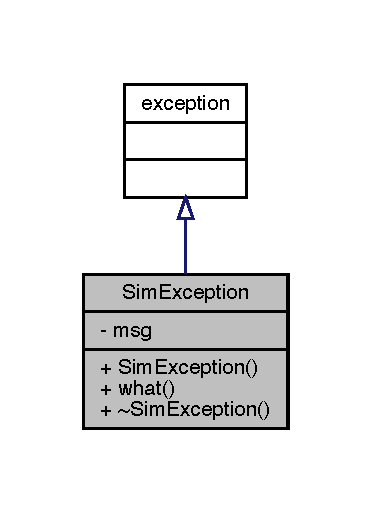
\includegraphics[width=178pt]{class_sim_exception__inherit__graph}
\end{center}
\end{figure}


Collaboration diagram for Sim\+Exception\+:
\nopagebreak
\begin{figure}[H]
\begin{center}
\leavevmode
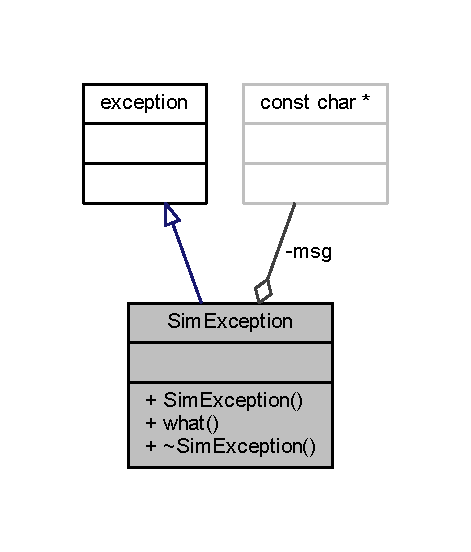
\includegraphics[width=226pt]{class_sim_exception__coll__graph}
\end{center}
\end{figure}
\subsection*{Public Member Functions}
\begin{DoxyCompactItemize}
\item 
\mbox{\hyperlink{class_sim_exception_a69f32113e1b068189e85f76b0340d073}{Sim\+Exception}} (const char $\ast$\mbox{\hyperlink{class_sim_exception_a1b07ee928b1ece4a807801a14713148a}{msg}})
\item 
virtual const char $\ast$ \mbox{\hyperlink{class_sim_exception_a7b759030340d1299a2eeb40c6f67a926}{what}} () const  throw ()
\item 
virtual \mbox{\hyperlink{class_sim_exception_a116fdf6821f150a43cefffd66d2b6506}{$\sim$\+Sim\+Exception}} ()
\end{DoxyCompactItemize}
\subsection*{Private Attributes}
\begin{DoxyCompactItemize}
\item 
const char $\ast$ \mbox{\hyperlink{class_sim_exception_a1b07ee928b1ece4a807801a14713148a}{msg}}
\end{DoxyCompactItemize}


\subsection{Constructor \& Destructor Documentation}
\mbox{\Hypertarget{class_sim_exception_a69f32113e1b068189e85f76b0340d073}\label{class_sim_exception_a69f32113e1b068189e85f76b0340d073}} 
\index{SimException@{SimException}!SimException@{SimException}}
\index{SimException@{SimException}!SimException@{SimException}}
\subsubsection{\texorpdfstring{SimException()}{SimException()}}
{\footnotesize\ttfamily Sim\+Exception\+::\+Sim\+Exception (\begin{DoxyParamCaption}\item[{const char $\ast$}]{msg }\end{DoxyParamCaption})}

\mbox{\Hypertarget{class_sim_exception_a116fdf6821f150a43cefffd66d2b6506}\label{class_sim_exception_a116fdf6821f150a43cefffd66d2b6506}} 
\index{SimException@{SimException}!````~SimException@{$\sim$SimException}}
\index{````~SimException@{$\sim$SimException}!SimException@{SimException}}
\subsubsection{\texorpdfstring{$\sim$SimException()}{~SimException()}}
{\footnotesize\ttfamily virtual Sim\+Exception\+::$\sim$\+Sim\+Exception (\begin{DoxyParamCaption}{ }\end{DoxyParamCaption})\hspace{0.3cm}{\ttfamily [virtual]}}



\subsection{Member Function Documentation}
\mbox{\Hypertarget{class_sim_exception_a7b759030340d1299a2eeb40c6f67a926}\label{class_sim_exception_a7b759030340d1299a2eeb40c6f67a926}} 
\index{SimException@{SimException}!what@{what}}
\index{what@{what}!SimException@{SimException}}
\subsubsection{\texorpdfstring{what()}{what()}}
{\footnotesize\ttfamily virtual const char$\ast$ Sim\+Exception\+::what (\begin{DoxyParamCaption}{ }\end{DoxyParamCaption}) const throw ( ) \hspace{0.3cm}{\ttfamily [virtual]}}



\subsection{Member Data Documentation}
\mbox{\Hypertarget{class_sim_exception_a1b07ee928b1ece4a807801a14713148a}\label{class_sim_exception_a1b07ee928b1ece4a807801a14713148a}} 
\index{SimException@{SimException}!msg@{msg}}
\index{msg@{msg}!SimException@{SimException}}
\subsubsection{\texorpdfstring{msg}{msg}}
{\footnotesize\ttfamily const char$\ast$ Sim\+Exception\+::msg\hspace{0.3cm}{\ttfamily [private]}}



The documentation for this class was generated from the following file\+:\begin{DoxyCompactItemize}
\item 
include/\mbox{\hyperlink{_sim_exception_8h}{Sim\+Exception.\+h}}\end{DoxyCompactItemize}

\hypertarget{class_tablet}{}\section{Tablet Class Reference}
\label{class_tablet}\index{Tablet@{Tablet}}


{\ttfamily \#include $<$Tablet.\+h$>$}



Inheritance diagram for Tablet\+:\nopagebreak
\begin{figure}[H]
\begin{center}
\leavevmode
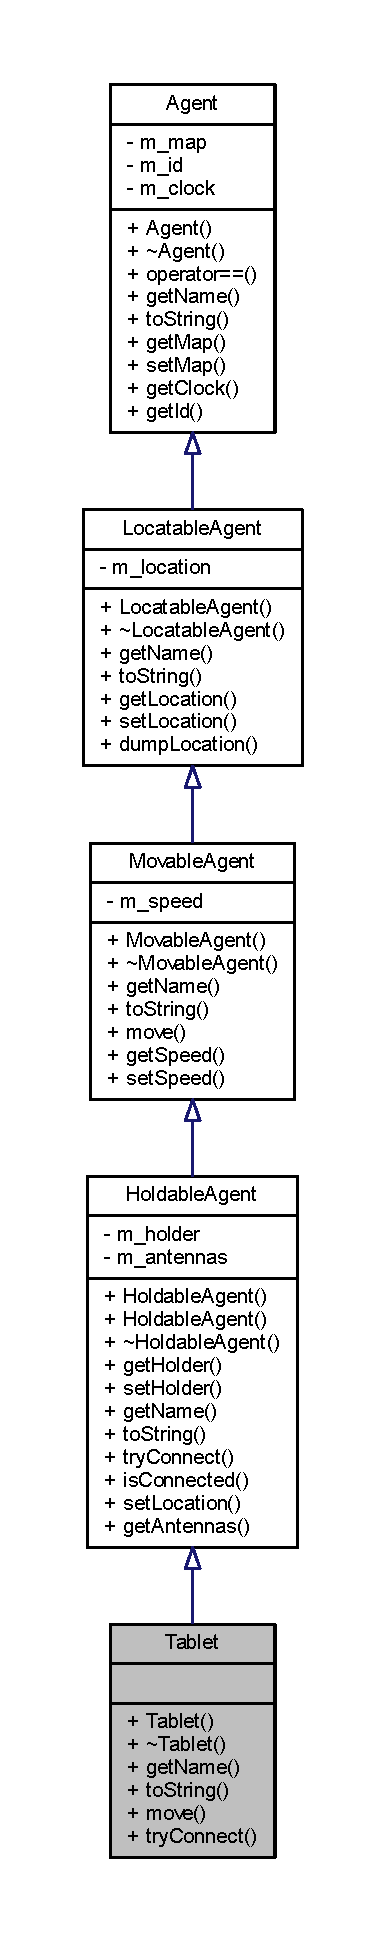
\includegraphics[height=550pt]{class_tablet__inherit__graph}
\end{center}
\end{figure}


Collaboration diagram for Tablet\+:\nopagebreak
\begin{figure}[H]
\begin{center}
\leavevmode
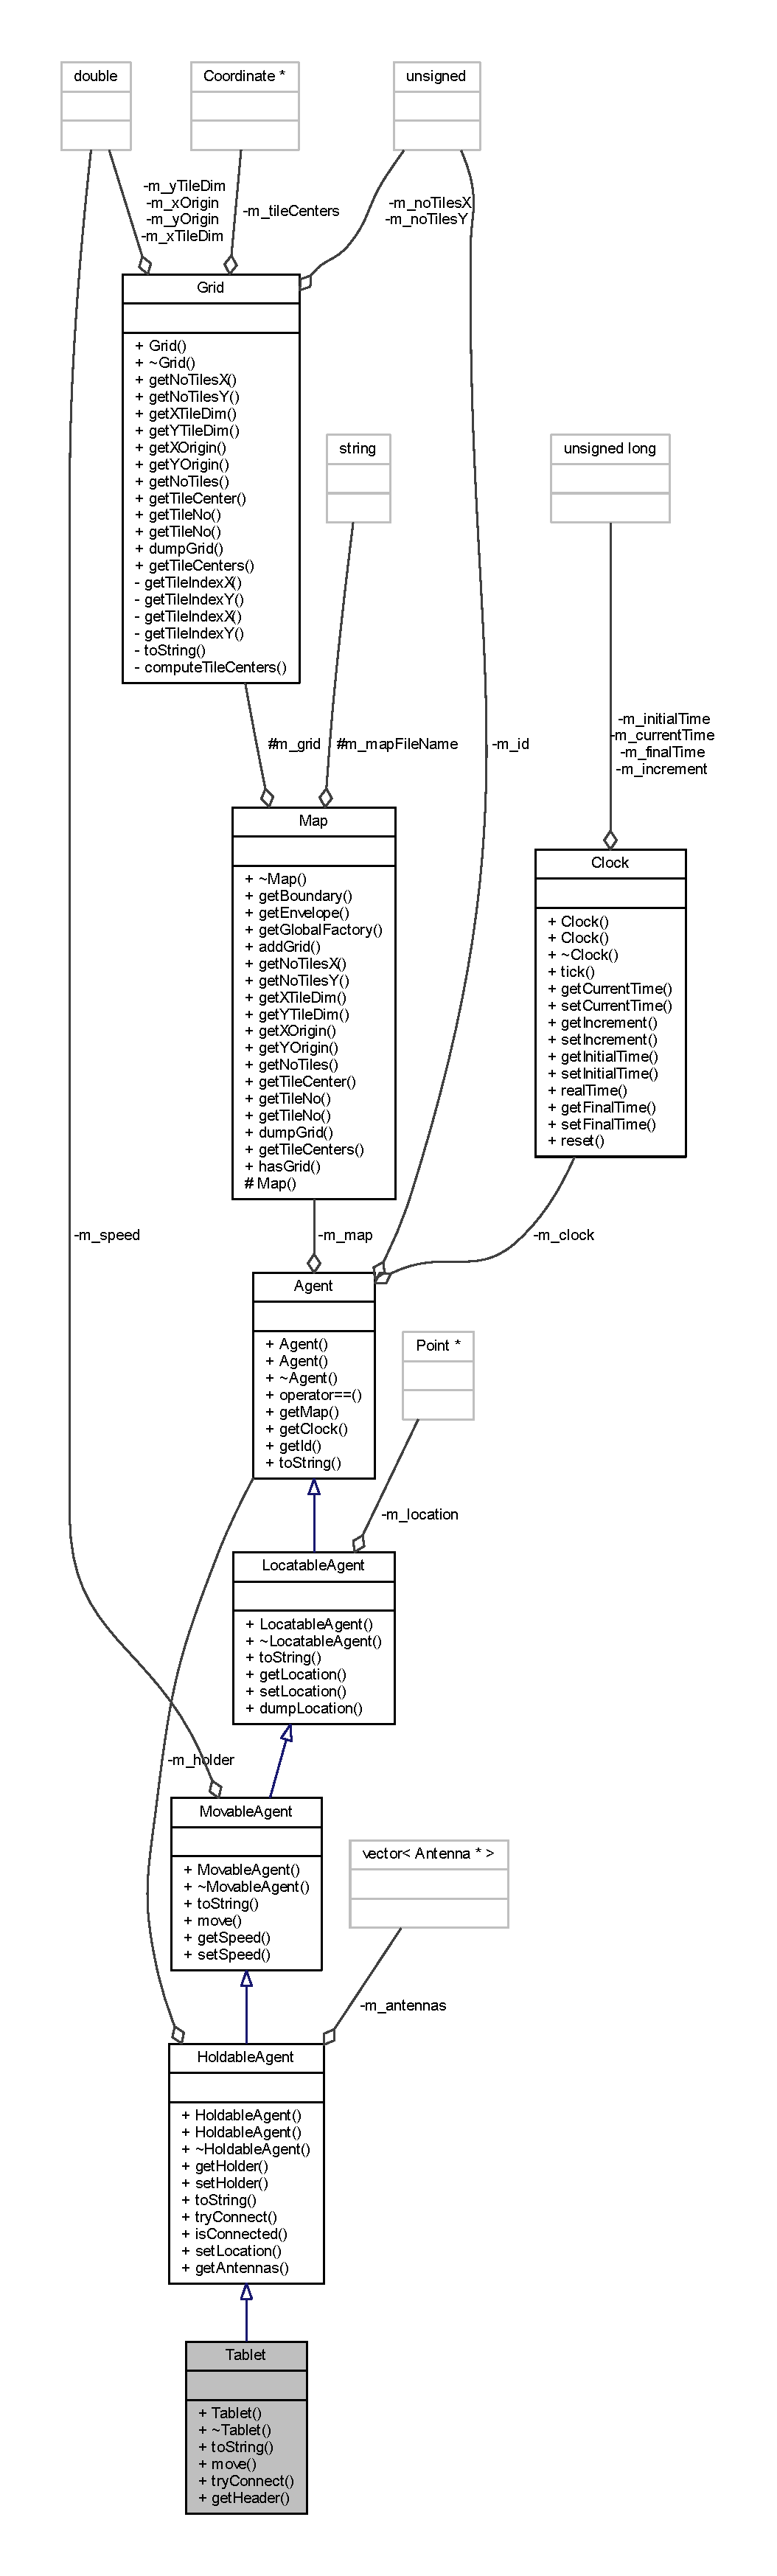
\includegraphics[height=550pt]{class_tablet__coll__graph}
\end{center}
\end{figure}
\subsection*{Public Member Functions}
\begin{DoxyCompactItemize}
\item 
\hyperlink{class_tablet_af457c0988b7a768659a284e16be58dc6}{Tablet} (const \hyperlink{class_map}{Map} $\ast$m, const unsigned long id, Point $\ast$init\+Position, const \hyperlink{class_clock}{Clock} $\ast$clock)
\item 
virtual \hyperlink{class_tablet_ac18d46eafd643e66dde81a3fefadab89}{$\sim$\+Tablet} ()
\item 
const string \hyperlink{class_tablet_adc7196aaee1e9714236b7cd8825d5826}{get\+Name} () const override
\item 
const string \hyperlink{class_tablet_a3fae01e7d526699476221c6a686a4fba}{to\+String} () const override
\item 
Point $\ast$ \hyperlink{class_tablet_ab1b8c7591be0c6ea118c8ab1c17839bb}{move} () override
\item 
bool \hyperlink{class_tablet_a2328422e1706dfeb2b51a6960e6879f0}{try\+Connect} () override
\end{DoxyCompactItemize}
\subsection*{Additional Inherited Members}


\subsection{Constructor \& Destructor Documentation}
\mbox{\Hypertarget{class_tablet_af457c0988b7a768659a284e16be58dc6}\label{class_tablet_af457c0988b7a768659a284e16be58dc6}} 
\index{Tablet@{Tablet}!Tablet@{Tablet}}
\index{Tablet@{Tablet}!Tablet@{Tablet}}
\subsubsection{\texorpdfstring{Tablet()}{Tablet()}}
{\footnotesize\ttfamily Tablet\+::\+Tablet (\begin{DoxyParamCaption}\item[{const \hyperlink{class_map}{Map} $\ast$}]{m,  }\item[{const unsigned long}]{id,  }\item[{Point $\ast$}]{init\+Position,  }\item[{const \hyperlink{class_clock}{Clock} $\ast$}]{clock }\end{DoxyParamCaption})\hspace{0.3cm}{\ttfamily [explicit]}}

Builds a new \hyperlink{class_tablet}{Tablet} object with the parameters provided by the user. 
\begin{DoxyParams}{Parameters}
{\em m} & a pointer to a \hyperlink{class_map}{Map} object used for simulation. \\
\hline
{\em id} & the id of the tablet. \\
\hline
{\em init\+Position} & the initial location on map. \\
\hline
{\em clock} & a pointer to a \hyperlink{class_clock}{Clock} object used for simulation.. \\
\hline
\end{DoxyParams}
\mbox{\Hypertarget{class_tablet_ac18d46eafd643e66dde81a3fefadab89}\label{class_tablet_ac18d46eafd643e66dde81a3fefadab89}} 
\index{Tablet@{Tablet}!````~Tablet@{$\sim$\+Tablet}}
\index{````~Tablet@{$\sim$\+Tablet}!Tablet@{Tablet}}
\subsubsection{\texorpdfstring{$\sim$\+Tablet()}{~Tablet()}}
{\footnotesize\ttfamily virtual Tablet\+::$\sim$\+Tablet (\begin{DoxyParamCaption}{ }\end{DoxyParamCaption})\hspace{0.3cm}{\ttfamily [virtual]}}

The default destructor. 

\subsection{Member Function Documentation}
\mbox{\Hypertarget{class_tablet_adc7196aaee1e9714236b7cd8825d5826}\label{class_tablet_adc7196aaee1e9714236b7cd8825d5826}} 
\index{Tablet@{Tablet}!get\+Name@{get\+Name}}
\index{get\+Name@{get\+Name}!Tablet@{Tablet}}
\subsubsection{\texorpdfstring{get\+Name()}{getName()}}
{\footnotesize\ttfamily const string Tablet\+::get\+Name (\begin{DoxyParamCaption}{ }\end{DoxyParamCaption}) const\hspace{0.3cm}{\ttfamily [override]}, {\ttfamily [virtual]}}

Returns the name of this class. \begin{DoxyReturn}{Returns}
the name of this class. 
\end{DoxyReturn}


Reimplemented from \hyperlink{class_holdable_agent_ab330bb40de51a957ef8826af629f94a2}{Holdable\+Agent}.

\mbox{\Hypertarget{class_tablet_ab1b8c7591be0c6ea118c8ab1c17839bb}\label{class_tablet_ab1b8c7591be0c6ea118c8ab1c17839bb}} 
\index{Tablet@{Tablet}!move@{move}}
\index{move@{move}!Tablet@{Tablet}}
\subsubsection{\texorpdfstring{move()}{move()}}
{\footnotesize\ttfamily Point$\ast$ Tablet\+::move (\begin{DoxyParamCaption}{ }\end{DoxyParamCaption})\hspace{0.3cm}{\ttfamily [inline]}, {\ttfamily [override]}, {\ttfamily [virtual]}}

Makes a step on the map according to an algorithm. The direction and the length of the step is determined by the displacement strategy and by the \hyperlink{class_person}{Person} object who owns this phone. The displacement strategy is set at the \hyperlink{class_person}{Person} object creation and currently two strategies are supported\+: \hyperlink{class_random_walk_displacement}{Random\+Walk\+Displacement} and \hyperlink{class_random_walk_drift_displacement}{Random\+Walk\+Drift\+Displacement}. \hyperlink{class_random_walk_displacement}{Random\+Walk\+Displacement} means that at each time instant the direction is generated as a uniformly distributed random value and the step length is computed multiplying the speed with the time interval set in the simulation configuration file. If a step projects it outside the map, it stops on the boundary. \hyperlink{class_random_walk_drift_displacement}{Random\+Walk\+Drift\+Displacement} means that there is a preference in the direction of the movement. There are two constants defined, S\+I\+M\+\_\+\+T\+R\+E\+N\+D\+\_\+\+A\+N\+G\+L\+E\+\_\+1 and S\+I\+M\+\_\+\+T\+R\+E\+N\+D\+\_\+\+A\+N\+G\+L\+E\+\_\+2 (3\+P\+I/4 and 5\+P\+I/4), and in the first half of the simulation the direction is generated as a normal distributed random value with the mean equals to S\+I\+M\+\_\+\+T\+R\+E\+N\+D\+\_\+\+A\+N\+G\+L\+E\+\_\+1 and sd = 0.\+1 while during the second half of the simulation it is generated as a normal distributed random value with the mean equals to S\+I\+M\+\_\+\+T\+R\+E\+N\+D\+\_\+\+A\+N\+G\+L\+E\+\_\+2 and the same sd. Again, any kind of \hyperlink{class_movable_agent}{Movable\+Agent} can only move inside the map boundary. If a step projects it outside the map, it stops on the boundary. \begin{DoxyReturn}{Returns}
the final location after the displacement. 
\end{DoxyReturn}


Implements \hyperlink{class_movable_agent_a88b617f0e78c817634e5b587da045ab0}{Movable\+Agent}.

Here is the call graph for this function\+:\nopagebreak
\begin{figure}[H]
\begin{center}
\leavevmode
\includegraphics[width=327pt]{class_tablet_ab1b8c7591be0c6ea118c8ab1c17839bb_cgraph}
\end{center}
\end{figure}
\mbox{\Hypertarget{class_tablet_a3fae01e7d526699476221c6a686a4fba}\label{class_tablet_a3fae01e7d526699476221c6a686a4fba}} 
\index{Tablet@{Tablet}!to\+String@{to\+String}}
\index{to\+String@{to\+String}!Tablet@{Tablet}}
\subsubsection{\texorpdfstring{to\+String()}{toString()}}
{\footnotesize\ttfamily const string Tablet\+::to\+String (\begin{DoxyParamCaption}{ }\end{DoxyParamCaption}) const\hspace{0.3cm}{\ttfamily [override]}, {\ttfamily [virtual]}}

Builds a human readable representation of this class. \begin{DoxyReturn}{Returns}
a human readable representation of this class. 
\end{DoxyReturn}


Reimplemented from \hyperlink{class_holdable_agent_a2c581226b8994f24b6b2306ae17dbb52}{Holdable\+Agent}.

\mbox{\Hypertarget{class_tablet_a2328422e1706dfeb2b51a6960e6879f0}\label{class_tablet_a2328422e1706dfeb2b51a6960e6879f0}} 
\index{Tablet@{Tablet}!try\+Connect@{try\+Connect}}
\index{try\+Connect@{try\+Connect}!Tablet@{Tablet}}
\subsubsection{\texorpdfstring{try\+Connect()}{tryConnect()}}
{\footnotesize\ttfamily bool Tablet\+::try\+Connect (\begin{DoxyParamCaption}{ }\end{DoxyParamCaption})\hspace{0.3cm}{\ttfamily [override]}, {\ttfamily [virtual]}}

Called after the tablet changes location on the map, tries to connect to an antenna. \begin{DoxyReturn}{Returns}
true if the connection succeeds, false otherwise. 
\end{DoxyReturn}


Implements \hyperlink{class_holdable_agent_a0789d757d81b43ee016e9362046f6dea}{Holdable\+Agent}.

Here is the caller graph for this function\+:\nopagebreak
\begin{figure}[H]
\begin{center}
\leavevmode
\includegraphics[width=283pt]{class_tablet_a2328422e1706dfeb2b51a6960e6879f0_icgraph}
\end{center}
\end{figure}


The documentation for this class was generated from the following file\+:\begin{DoxyCompactItemize}
\item 
include/\hyperlink{_tablet_8h}{Tablet.\+h}\end{DoxyCompactItemize}

\section{World Class Reference}
\label{class_world}\index{World@{World}}


{\ttfamily \#include $<$World.\+h$>$}

\subsection*{Public Member Functions}
\begin{DoxyCompactItemize}
\item 
\textbf{ World} (\textbf{ Map} $\ast$map, int num\+Persons, int num\+Antennas, int num\+Mobile\+Phones)
\item 
\textbf{ World} (\textbf{ Map} $\ast$map, int num\+Persons, const string \&config\+Antennas\+File, int num\+Mobile\+Phones) noexcept(false)
\item 
\textbf{ World} (\textbf{ Map} $\ast$map, const string \&config\+Persons\+File\+Name, const string \&config\+Antennas\+File\+Name, const string \&config\+Simulation\+File\+Name) noexcept(false)
\item 
virtual \textbf{ $\sim$\+World} ()
\item 
void \textbf{ run\+Simulation} (string \&persons\+File, string \&antennas\+File) noexcept(false)
\item 
void \textbf{ dump\+State} ()
\item 
unsigned int \textbf{ get\+Current\+Time} ()
\item 
\textbf{ Agents\+Collection} $\ast$ \textbf{ get\+Agents} () const
\item 
void \textbf{ set\+Agents} (\textbf{ Agents\+Collection} $\ast$agents)
\item 
\textbf{ Clock} $\ast$ \textbf{ get\+Clock} () const
\item 
void \textbf{ set\+Clock} (\textbf{ Clock} $\ast$clock)
\item 
\textbf{ Map} $\ast$ \textbf{ get\+Map} () const
\item 
void \textbf{ set\+Map} (\textbf{ Map} $\ast$map)
\end{DoxyCompactItemize}
\subsection*{Private Member Functions}
\begin{DoxyCompactItemize}
\item 
vector$<$ \textbf{ Person} $\ast$ $>$ \textbf{ generate\+Population} (unsigned long num\+Persons)
\item 
vector$<$ \textbf{ Person} $\ast$ $>$ \textbf{ generate\+Population} (unsigned long num\+Persons, vector$<$ double $>$ params, \textbf{ Person\+::\+Age\+Distributions} age\+\_\+distribution, double male\+\_\+share, double prob\+\_\+mobile\+\_\+phone, double speed\+\_\+walk, double speed\+\_\+car)
\item 
vector$<$ \textbf{ Antenna} $\ast$ $>$ \textbf{ generate\+Antennas} (unsigned long num\+Antennas)
\item 
vector$<$ \textbf{ Antenna} $\ast$ $>$ \textbf{ parse\+Antennas} (const string \&config\+Antennas\+File) noexcept(false)
\item 
vector$<$ \textbf{ Person} $\ast$ $>$ \textbf{ parse\+Persons} (const string \&persons\+File\+Name) noexcept(false)
\item 
vector$<$ \textbf{ Mobile\+Phone} $\ast$ $>$ \textbf{ generate\+Mobile\+Phones} (int num\+Mobile\+Phones, \textbf{ Holdable\+Agent\+::\+C\+O\+N\+N\+E\+C\+T\+I\+O\+N\+\_\+\+T\+Y\+PE} conn\+Type)
\item 
void \textbf{ parse\+Simulation\+File} (const string \&config\+Simulation\+File\+Name) noexcept(false)
\end{DoxyCompactItemize}
\subsection*{Private Attributes}
\begin{DoxyCompactItemize}
\item 
\textbf{ Map} $\ast$ \textbf{ m\+\_\+map}
\item 
\textbf{ Agents\+Collection} $\ast$ \textbf{ m\+\_\+agents\+Collection}
\item 
\textbf{ Clock} $\ast$ \textbf{ m\+\_\+clock}
\item 
unsigned long \textbf{ m\+\_\+start\+Time}
\item 
unsigned long \textbf{ m\+\_\+end\+Time}
\item 
unsigned long \textbf{ m\+\_\+time\+Increment}
\item 
\textbf{ Holdable\+Agent\+::\+C\+O\+N\+N\+E\+C\+T\+I\+O\+N\+\_\+\+T\+Y\+PE} \textbf{ m\+\_\+conn\+Type}
\item 
\textbf{ Movement\+Type} \textbf{ m\+\_\+mv\+Type}
\end{DoxyCompactItemize}


\subsection{Detailed Description}


Definition at line 28 of file World.\+h.



\subsection{Constructor \& Destructor Documentation}
\mbox{\label{class_world_a94871f094bb3eabb67f5bd1b10396832}} 
\index{World@{World}!World@{World}}
\index{World@{World}!World@{World}}
\subsubsection{World()\hspace{0.1cm}{\footnotesize\ttfamily [1/3]}}
{\footnotesize\ttfamily World\+::\+World (\begin{DoxyParamCaption}\item[{\textbf{ Map} $\ast$}]{map,  }\item[{int}]{num\+Persons,  }\item[{int}]{num\+Antennas,  }\item[{int}]{num\+Mobile\+Phones }\end{DoxyParamCaption})}

Default constructor 

Definition at line 37 of file World.\+cpp.

\mbox{\label{class_world_a5a02572c10d750037a8c604a7d806550}} 
\index{World@{World}!World@{World}}
\index{World@{World}!World@{World}}
\subsubsection{World()\hspace{0.1cm}{\footnotesize\ttfamily [2/3]}}
{\footnotesize\ttfamily World\+::\+World (\begin{DoxyParamCaption}\item[{\textbf{ Map} $\ast$}]{map,  }\item[{int}]{num\+Persons,  }\item[{const string \&}]{config\+Antennas\+File,  }\item[{int}]{num\+Mobile\+Phones }\end{DoxyParamCaption})\hspace{0.3cm}{\ttfamily [noexcept]}}



Definition at line 61 of file World.\+cpp.

\mbox{\label{class_world_a6376bd8ac7c88b8e01e7cca06d9bb18a}} 
\index{World@{World}!World@{World}}
\index{World@{World}!World@{World}}
\subsubsection{World()\hspace{0.1cm}{\footnotesize\ttfamily [3/3]}}
{\footnotesize\ttfamily World\+::\+World (\begin{DoxyParamCaption}\item[{\textbf{ Map} $\ast$}]{map,  }\item[{const string \&}]{config\+Persons\+File\+Name,  }\item[{const string \&}]{config\+Antennas\+File\+Name,  }\item[{const string \&}]{config\+Simulation\+File\+Name }\end{DoxyParamCaption})\hspace{0.3cm}{\ttfamily [noexcept]}}



Definition at line 84 of file World.\+cpp.

\mbox{\label{class_world_a8c73fba541a5817fff65147ba47cd827}} 
\index{World@{World}!````~World@{$\sim$World}}
\index{````~World@{$\sim$World}!World@{World}}
\subsubsection{$\sim$World()}
{\footnotesize\ttfamily World\+::$\sim$\+World (\begin{DoxyParamCaption}{ }\end{DoxyParamCaption})\hspace{0.3cm}{\ttfamily [virtual]}}

Default destructor 

Definition at line 104 of file World.\+cpp.



References m\+\_\+agents\+Collection, and m\+\_\+clock.



\subsection{Member Function Documentation}
\mbox{\label{class_world_abb6faf5385d3960dca29ee9390460eea}} 
\index{World@{World}!dumpState@{dumpState}}
\index{dumpState@{dumpState}!World@{World}}
\subsubsection{dumpState()}
{\footnotesize\ttfamily void World\+::dump\+State (\begin{DoxyParamCaption}{ }\end{DoxyParamCaption})}

\mbox{\label{class_world_a6cb3aa7d814b3d6302ea984889179eac}} 
\index{World@{World}!generateAntennas@{generateAntennas}}
\index{generateAntennas@{generateAntennas}!World@{World}}
\subsubsection{generateAntennas()}
{\footnotesize\ttfamily vector$<$ \textbf{ Antenna} $\ast$ $>$ World\+::generate\+Antennas (\begin{DoxyParamCaption}\item[{unsigned long}]{num\+Antennas }\end{DoxyParamCaption})\hspace{0.3cm}{\ttfamily [private]}}



Definition at line 208 of file World.\+cpp.



References Constants\+::\+A\+N\+T\+E\+N\+N\+A\+\_\+\+P\+O\+W\+ER, Constants\+::\+A\+T\+T\+\_\+\+F\+A\+C\+T\+OR, utils\+::generate\+Points(), get\+Map(), I\+D\+Generator\+::instance(), m\+\_\+clock, Constants\+::\+M\+A\+X\+\_\+\+C\+O\+N\+N\+E\+C\+T\+I\+O\+NS, I\+D\+Generator\+::next(), O\+M\+N\+I\+D\+I\+R\+E\+C\+T\+I\+O\+N\+AL, Constants\+::\+S\+\_\+\+M\+ID, and Constants\+::\+S\+\_\+\+S\+T\+E\+EP.

\mbox{\label{class_world_a478f62a296d9a7b6587c116aab6563c6}} 
\index{World@{World}!generateMobilePhones@{generateMobilePhones}}
\index{generateMobilePhones@{generateMobilePhones}!World@{World}}
\subsubsection{generateMobilePhones()}
{\footnotesize\ttfamily vector$<$ \textbf{ Mobile\+Phone} $\ast$ $>$ World\+::generate\+Mobile\+Phones (\begin{DoxyParamCaption}\item[{int}]{num\+Mobile\+Phones,  }\item[{\textbf{ Holdable\+Agent\+::\+C\+O\+N\+N\+E\+C\+T\+I\+O\+N\+\_\+\+T\+Y\+PE}}]{conn\+Type }\end{DoxyParamCaption})\hspace{0.3cm}{\ttfamily [private]}}



Definition at line 228 of file World.\+cpp.



References Agents\+Collection\+::add\+Agent(), get\+Map(), I\+D\+Generator\+::instance(), m\+\_\+agents\+Collection, m\+\_\+clock, I\+D\+Generator\+::next(), Constants\+::\+P\+O\+W\+E\+R\+\_\+\+T\+H\+R\+E\+S\+H\+O\+LD, and Constants\+::\+Q\+U\+A\+L\+I\+T\+Y\+\_\+\+T\+H\+R\+E\+S\+H\+O\+LD.



Referenced by generate\+Population().

\mbox{\label{class_world_a76bc2ffba54afefbb84b2f6fc781b629}} 
\index{World@{World}!generatePopulation@{generatePopulation}}
\index{generatePopulation@{generatePopulation}!World@{World}}
\subsubsection{generatePopulation()\hspace{0.1cm}{\footnotesize\ttfamily [1/2]}}
{\footnotesize\ttfamily vector$<$ \textbf{ Person} $\ast$ $>$ World\+::generate\+Population (\begin{DoxyParamCaption}\item[{unsigned long}]{num\+Persons }\end{DoxyParamCaption})\hspace{0.3cm}{\ttfamily [private]}}



Definition at line 189 of file World.\+cpp.



References Random\+Number\+Generator\+::generate\+Normal2\+Double(), utils\+::generate\+Points(), Random\+Number\+Generator\+::generate\+Uniform\+Int(), get\+Map(), I\+D\+Generator\+::instance(), Random\+Number\+Generator\+::instance(), m\+\_\+clock, and I\+D\+Generator\+::next().

\mbox{\label{class_world_ac6bb92d77d6be53323a24b0fd825f986}} 
\index{World@{World}!generatePopulation@{generatePopulation}}
\index{generatePopulation@{generatePopulation}!World@{World}}
\subsubsection{generatePopulation()\hspace{0.1cm}{\footnotesize\ttfamily [2/2]}}
{\footnotesize\ttfamily vector$<$ \textbf{ Person} $\ast$ $>$ World\+::generate\+Population (\begin{DoxyParamCaption}\item[{unsigned long}]{num\+Persons,  }\item[{vector$<$ double $>$}]{params,  }\item[{\textbf{ Person\+::\+Age\+Distributions}}]{age\+\_\+distribution,  }\item[{double}]{male\+\_\+share,  }\item[{double}]{prob\+\_\+mobile\+\_\+phone,  }\item[{double}]{speed\+\_\+walk,  }\item[{double}]{speed\+\_\+car }\end{DoxyParamCaption})\hspace{0.3cm}{\ttfamily [private]}}



Definition at line 364 of file World.\+cpp.



References Person\+::add\+Device(), Random\+Number\+Generator\+::generate\+Binomial\+Int(), generate\+Mobile\+Phones(), Random\+Number\+Generator\+::generate\+Normal\+Double(), utils\+::generate\+Points(), Random\+Number\+Generator\+::generate\+Truncated\+Normal\+Double(), Random\+Number\+Generator\+::generate\+Uniform\+Double(), get\+Map(), I\+D\+Generator\+::instance(), Random\+Number\+Generator\+::instance(), m\+\_\+clock, m\+\_\+conn\+Type, and I\+D\+Generator\+::next().

\mbox{\label{class_world_a365cced3803fd8390a781619b61e2818}} 
\index{World@{World}!getAgents@{getAgents}}
\index{getAgents@{getAgents}!World@{World}}
\subsubsection{getAgents()}
{\footnotesize\ttfamily \textbf{ Agents\+Collection} $\ast$ World\+::get\+Agents (\begin{DoxyParamCaption}{ }\end{DoxyParamCaption}) const}



Definition at line 165 of file World.\+cpp.



References m\+\_\+agents\+Collection.

\mbox{\label{class_world_a521915088db371c5730093331a74b080}} 
\index{World@{World}!getClock@{getClock}}
\index{getClock@{getClock}!World@{World}}
\subsubsection{getClock()}
{\footnotesize\ttfamily \textbf{ Clock} $\ast$ World\+::get\+Clock (\begin{DoxyParamCaption}{ }\end{DoxyParamCaption}) const}



Definition at line 173 of file World.\+cpp.



References m\+\_\+clock.

\mbox{\label{class_world_af33b51dff9edc6770890ef579700d959}} 
\index{World@{World}!getCurrentTime@{getCurrentTime}}
\index{getCurrentTime@{getCurrentTime}!World@{World}}
\subsubsection{getCurrentTime()}
{\footnotesize\ttfamily unsigned int World\+::get\+Current\+Time (\begin{DoxyParamCaption}{ }\end{DoxyParamCaption})}



Definition at line 161 of file World.\+cpp.



References Clock\+::get\+Current\+Time(), and m\+\_\+clock.

\mbox{\label{class_world_a5b82e6105d8f4b3d757eb7da6d65205a}} 
\index{World@{World}!getMap@{getMap}}
\index{getMap@{getMap}!World@{World}}
\subsubsection{getMap()}
{\footnotesize\ttfamily \textbf{ Map} $\ast$ World\+::get\+Map (\begin{DoxyParamCaption}{ }\end{DoxyParamCaption}) const}



Definition at line 181 of file World.\+cpp.



References m\+\_\+map.



Referenced by generate\+Antennas(), generate\+Mobile\+Phones(), and generate\+Population().

\mbox{\label{class_world_aaf31e06b9b5a40a4338164e0f641f7d0}} 
\index{World@{World}!parseAntennas@{parseAntennas}}
\index{parseAntennas@{parseAntennas}!World@{World}}
\subsubsection{parseAntennas()}
{\footnotesize\ttfamily vector$<$ \textbf{ Antenna} $\ast$ $>$ World\+::parse\+Antennas (\begin{DoxyParamCaption}\item[{const string \&}]{config\+Antennas\+File }\end{DoxyParamCaption})\hspace{0.3cm}{\ttfamily [private]}, {\ttfamily [noexcept]}}



Definition at line 240 of file World.\+cpp.



References tinyxml2\+::\+X\+M\+L\+Node\+::\+First\+Child\+Element(), utils\+::get\+First\+Child\+Element(), I\+D\+Generator\+::instance(), tinyxml2\+::\+X\+M\+L\+Document\+::\+Load\+File(), tinyxml2\+::\+X\+M\+L\+Element\+::\+Name(), I\+D\+Generator\+::next(), tinyxml2\+::\+X\+M\+L\+Node\+::\+Next\+Sibling\+Element(), and tinyxml2\+::\+X\+M\+L\+\_\+\+S\+U\+C\+C\+E\+SS.

\mbox{\label{class_world_a8bdce1dbc8d7a653d63a59674e283622}} 
\index{World@{World}!parsePersons@{parsePersons}}
\index{parsePersons@{parsePersons}!World@{World}}
\subsubsection{parsePersons()}
{\footnotesize\ttfamily vector$<$ \textbf{ Person} $\ast$ $>$ World\+::parse\+Persons (\begin{DoxyParamCaption}\item[{const string \&}]{persons\+File\+Name }\end{DoxyParamCaption})\hspace{0.3cm}{\ttfamily [private]}, {\ttfamily [noexcept]}}



Definition at line 265 of file World.\+cpp.



References tinyxml2\+::\+X\+M\+L\+Node\+::\+First\+Child\+Element(), utils\+::get\+First\+Child\+Element(), utils\+::get\+Node(), tinyxml2\+::\+X\+M\+L\+Document\+::\+Load\+File(), tinyxml2\+::\+X\+M\+L\+Node\+::\+To\+Text(), tinyxml2\+::\+X\+M\+L\+Node\+::\+Value(), and tinyxml2\+::\+X\+M\+L\+\_\+\+S\+U\+C\+C\+E\+SS.

\mbox{\label{class_world_a7f00dc79cc98281dbf7c51fb2c83e8d6}} 
\index{World@{World}!parseSimulationFile@{parseSimulationFile}}
\index{parseSimulationFile@{parseSimulationFile}!World@{World}}
\subsubsection{parseSimulationFile()}
{\footnotesize\ttfamily void World\+::parse\+Simulation\+File (\begin{DoxyParamCaption}\item[{const string \&}]{config\+Simulation\+File\+Name }\end{DoxyParamCaption})\hspace{0.3cm}{\ttfamily [private]}, {\ttfamily [noexcept]}}



Definition at line 331 of file World.\+cpp.



References tinyxml2\+::\+X\+M\+L\+Node\+::\+First\+Child\+Element(), utils\+::get\+Node(), tinyxml2\+::\+X\+M\+L\+Document\+::\+Load\+File(), R\+A\+N\+D\+O\+M\+\_\+\+W\+A\+LK, tinyxml2\+::\+X\+M\+L\+Node\+::\+To\+Text(), U\+N\+K\+N\+O\+WN, tinyxml2\+::\+X\+M\+L\+Node\+::\+Value(), and tinyxml2\+::\+X\+M\+L\+\_\+\+S\+U\+C\+C\+E\+SS.

\mbox{\label{class_world_af8d69e177beec5a9cf3c200f292db7db}} 
\index{World@{World}!runSimulation@{runSimulation}}
\index{runSimulation@{runSimulation}!World@{World}}
\subsubsection{runSimulation()}
{\footnotesize\ttfamily void World\+::run\+Simulation (\begin{DoxyParamCaption}\item[{string \&}]{persons\+File,  }\item[{string \&}]{antennas\+File }\end{DoxyParamCaption})\hspace{0.3cm}{\ttfamily [noexcept]}}



Definition at line 111 of file World.\+cpp.



References Person\+::dump\+Devices(), Locatable\+Agent\+::dump\+Location(), and Person\+::move().

\mbox{\label{class_world_afa8e5c2943c72aa664590abbb024896b}} 
\index{World@{World}!setAgents@{setAgents}}
\index{setAgents@{setAgents}!World@{World}}
\subsubsection{setAgents()}
{\footnotesize\ttfamily void World\+::set\+Agents (\begin{DoxyParamCaption}\item[{\textbf{ Agents\+Collection} $\ast$}]{agents }\end{DoxyParamCaption})}



Definition at line 169 of file World.\+cpp.



References m\+\_\+agents\+Collection.

\mbox{\label{class_world_a52ebe3eed240fe4dd37915a1dad02efd}} 
\index{World@{World}!setClock@{setClock}}
\index{setClock@{setClock}!World@{World}}
\subsubsection{setClock()}
{\footnotesize\ttfamily void World\+::set\+Clock (\begin{DoxyParamCaption}\item[{\textbf{ Clock} $\ast$}]{clock }\end{DoxyParamCaption})}



Definition at line 177 of file World.\+cpp.



References m\+\_\+clock.

\mbox{\label{class_world_a9dc80487d5c2d1d4f2af0c1d7f015204}} 
\index{World@{World}!setMap@{setMap}}
\index{setMap@{setMap}!World@{World}}
\subsubsection{setMap()}
{\footnotesize\ttfamily void World\+::set\+Map (\begin{DoxyParamCaption}\item[{\textbf{ Map} $\ast$}]{map }\end{DoxyParamCaption})}



Definition at line 185 of file World.\+cpp.



References m\+\_\+map.



\subsection{Member Data Documentation}
\mbox{\label{class_world_ae1262689381f00828c0a639b7cbb52a3}} 
\index{World@{World}!m\_agentsCollection@{m\_agentsCollection}}
\index{m\_agentsCollection@{m\_agentsCollection}!World@{World}}
\subsubsection{m\_agentsCollection}
{\footnotesize\ttfamily \textbf{ Agents\+Collection}$\ast$ World\+::m\+\_\+agents\+Collection\hspace{0.3cm}{\ttfamily [private]}}



Definition at line 60 of file World.\+h.



Referenced by generate\+Mobile\+Phones(), get\+Agents(), set\+Agents(), and $\sim$\+World().

\mbox{\label{class_world_a8359eb424f01e41703faa0885a4414bf}} 
\index{World@{World}!m\_clock@{m\_clock}}
\index{m\_clock@{m\_clock}!World@{World}}
\subsubsection{m\_clock}
{\footnotesize\ttfamily \textbf{ Clock}$\ast$ World\+::m\+\_\+clock\hspace{0.3cm}{\ttfamily [private]}}



Definition at line 61 of file World.\+h.



Referenced by generate\+Antennas(), generate\+Mobile\+Phones(), generate\+Population(), get\+Clock(), get\+Current\+Time(), set\+Clock(), and $\sim$\+World().

\mbox{\label{class_world_afeac65cddcd1e1c4fa14a17efa35be06}} 
\index{World@{World}!m\_connType@{m\_connType}}
\index{m\_connType@{m\_connType}!World@{World}}
\subsubsection{m\_connType}
{\footnotesize\ttfamily \textbf{ Holdable\+Agent\+::\+C\+O\+N\+N\+E\+C\+T\+I\+O\+N\+\_\+\+T\+Y\+PE} World\+::m\+\_\+conn\+Type\hspace{0.3cm}{\ttfamily [private]}}



Definition at line 66 of file World.\+h.



Referenced by generate\+Population().

\mbox{\label{class_world_ab6b8ad11e4031f3072a78f00a66e9ec5}} 
\index{World@{World}!m\_endTime@{m\_endTime}}
\index{m\_endTime@{m\_endTime}!World@{World}}
\subsubsection{m\_endTime}
{\footnotesize\ttfamily unsigned long World\+::m\+\_\+end\+Time\hspace{0.3cm}{\ttfamily [private]}}



Definition at line 63 of file World.\+h.

\mbox{\label{class_world_ae1e6f62c5b282e94ffdcaab58fcb3fb4}} 
\index{World@{World}!m\_map@{m\_map}}
\index{m\_map@{m\_map}!World@{World}}
\subsubsection{m\_map}
{\footnotesize\ttfamily \textbf{ Map}$\ast$ World\+::m\+\_\+map\hspace{0.3cm}{\ttfamily [private]}}



Definition at line 58 of file World.\+h.



Referenced by get\+Map(), and set\+Map().

\mbox{\label{class_world_a9fcf012ce7262edf5646f0720ffd7666}} 
\index{World@{World}!m\_mvType@{m\_mvType}}
\index{m\_mvType@{m\_mvType}!World@{World}}
\subsubsection{m\_mvType}
{\footnotesize\ttfamily \textbf{ Movement\+Type} World\+::m\+\_\+mv\+Type\hspace{0.3cm}{\ttfamily [private]}}



Definition at line 67 of file World.\+h.

\mbox{\label{class_world_a5b46814e7da7222730be62154bf10008}} 
\index{World@{World}!m\_startTime@{m\_startTime}}
\index{m\_startTime@{m\_startTime}!World@{World}}
\subsubsection{m\_startTime}
{\footnotesize\ttfamily unsigned long World\+::m\+\_\+start\+Time\hspace{0.3cm}{\ttfamily [private]}}



Definition at line 62 of file World.\+h.

\mbox{\label{class_world_a97f773548fef49eb408115c097aa995d}} 
\index{World@{World}!m\_timeIncrement@{m\_timeIncrement}}
\index{m\_timeIncrement@{m\_timeIncrement}!World@{World}}
\subsubsection{m\_timeIncrement}
{\footnotesize\ttfamily unsigned long World\+::m\+\_\+time\+Increment\hspace{0.3cm}{\ttfamily [private]}}



Definition at line 64 of file World.\+h.



The documentation for this class was generated from the following files\+:\begin{DoxyCompactItemize}
\item 
include/\textbf{ World.\+h}\item 
src/\textbf{ World.\+cpp}\end{DoxyCompactItemize}

\chapter{File Documentation}
\hypertarget{_agent_8h}{}\section{include/\+Agent.h File Reference}
\label{_agent_8h}\index{include/Agent.h@{include/Agent.h}}
{\ttfamily \#include $<$Map.\+h$>$}\newline
{\ttfamily \#include $<$Clock.\+h$>$}\newline
{\ttfamily \#include $<$string$>$}\newline
Include dependency graph for Agent.\+h\+:\nopagebreak
\begin{figure}[H]
\begin{center}
\leavevmode
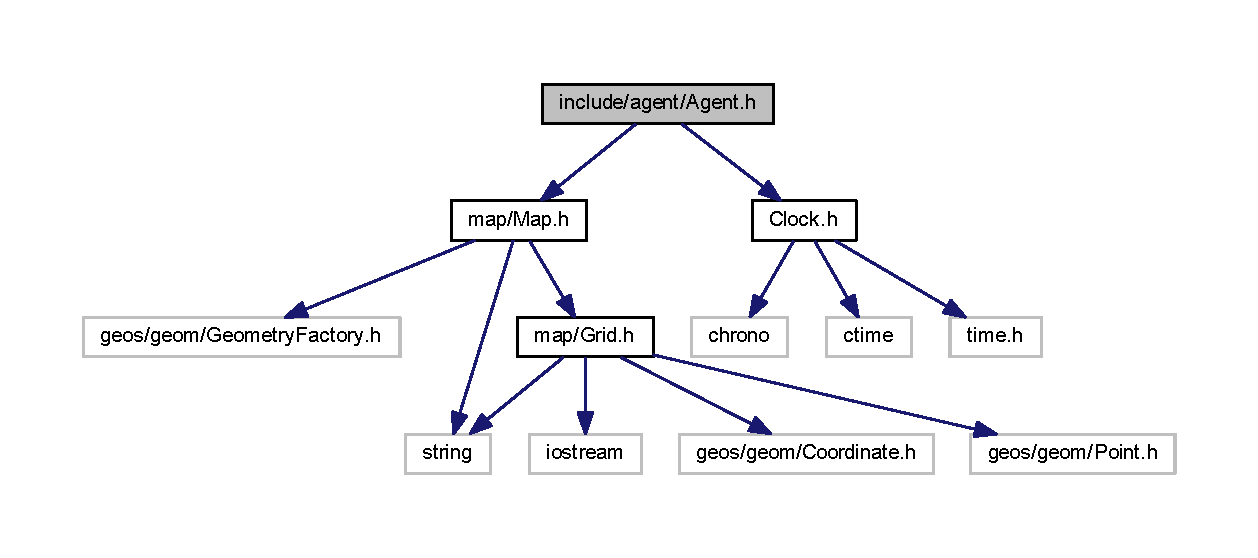
\includegraphics[width=350pt]{_agent_8h__incl}
\end{center}
\end{figure}
This graph shows which files directly or indirectly include this file\+:\nopagebreak
\begin{figure}[H]
\begin{center}
\leavevmode
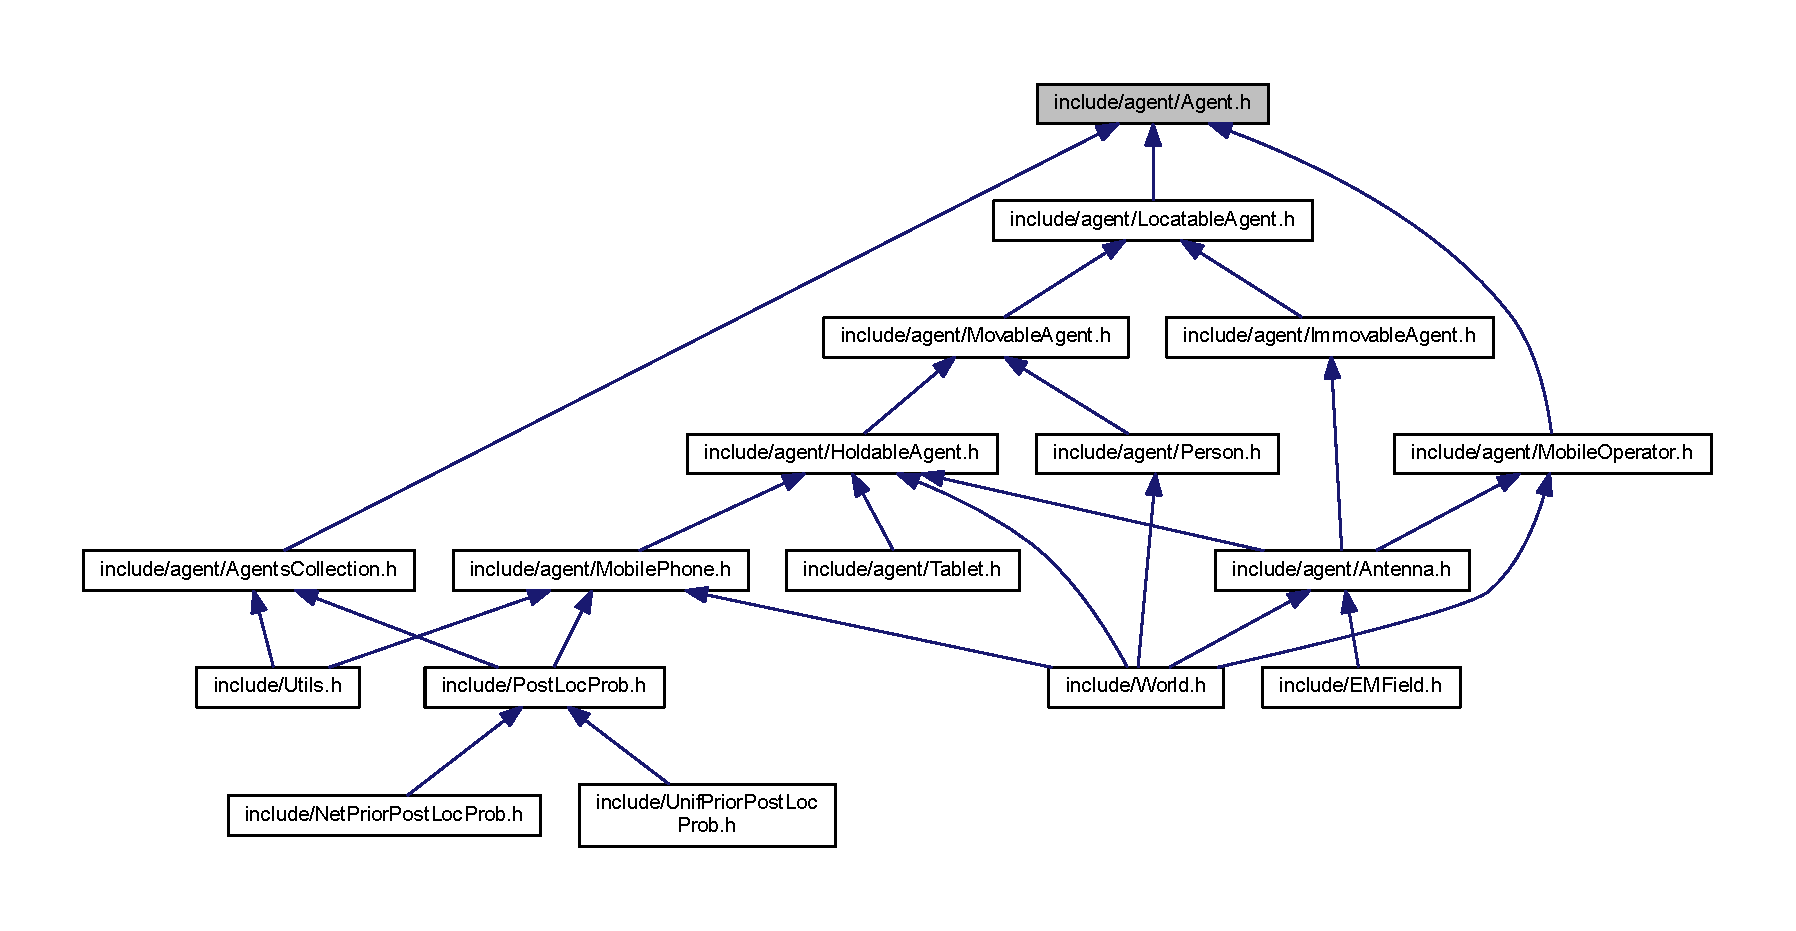
\includegraphics[width=350pt]{_agent_8h__dep__incl}
\end{center}
\end{figure}
\subsection*{Classes}
\begin{DoxyCompactItemize}
\item 
class \mbox{\hyperlink{class_agent}{Agent}}
\end{DoxyCompactItemize}

\hypertarget{_agents_collection_8h}{}\section{include/\+Agents\+Collection.h File Reference}
\label{_agents_collection_8h}\index{include/AgentsCollection.h@{include/AgentsCollection.h}}
{\ttfamily \#include $<$Agent.\+h$>$}\newline
{\ttfamily \#include $<$typeinfo$>$}\newline
{\ttfamily \#include $<$unordered\+\_\+map$>$}\newline
{\ttfamily \#include $<$vector$>$}\newline
Include dependency graph for Agents\+Collection.\+h\+:\nopagebreak
\begin{figure}[H]
\begin{center}
\leavevmode
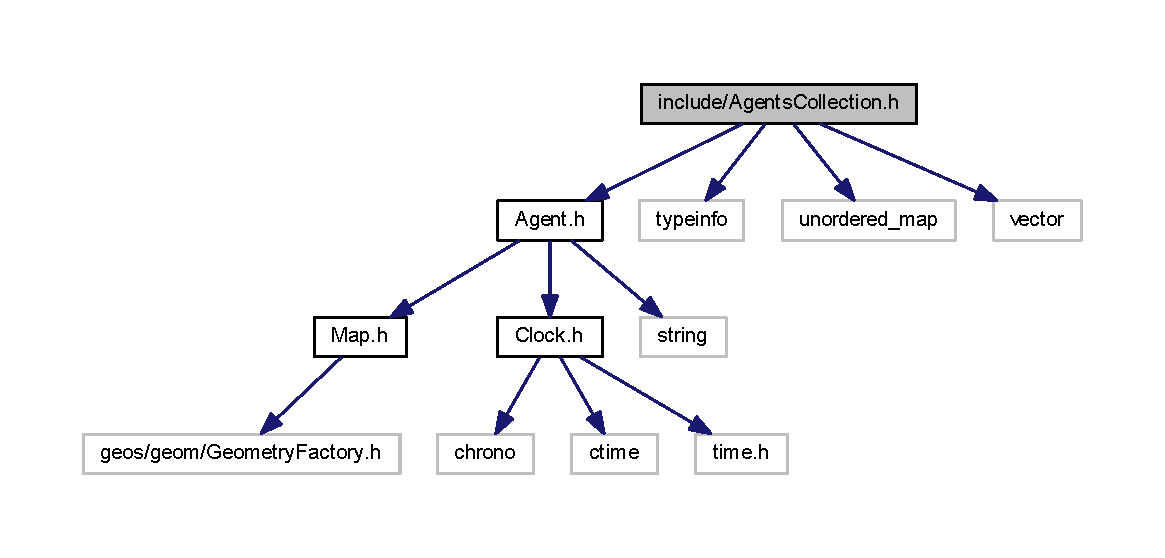
\includegraphics[width=350pt]{_agents_collection_8h__incl}
\end{center}
\end{figure}
This graph shows which files directly or indirectly include this file\+:\nopagebreak
\begin{figure}[H]
\begin{center}
\leavevmode
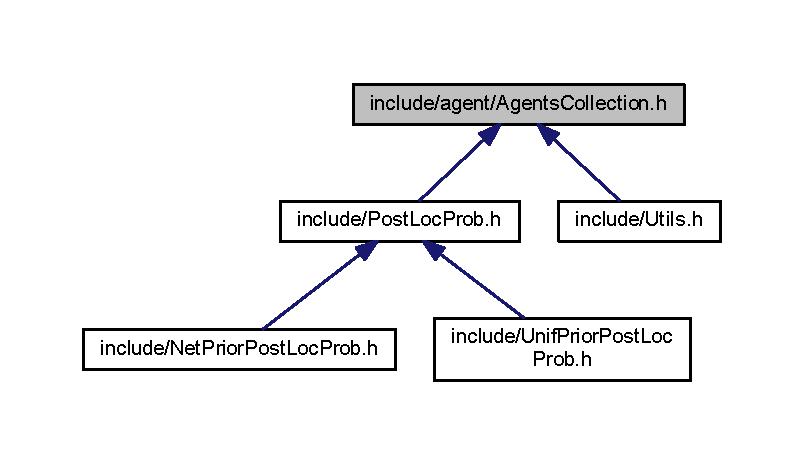
\includegraphics[width=269pt]{_agents_collection_8h__dep__incl}
\end{center}
\end{figure}
\subsection*{Classes}
\begin{DoxyCompactItemize}
\item 
class \mbox{\hyperlink{class_agents_collection}{Agents\+Collection}}
\end{DoxyCompactItemize}
\subsection*{Typedefs}
\begin{DoxyCompactItemize}
\item 
typedef unordered\+\_\+multimap$<$ string, \mbox{\hyperlink{class_agent}{Agent}} $\ast$ $>$\+::iterator \mbox{\hyperlink{_agents_collection_8h_afde47bc45d604b8b8c72755072376679}{um\+\_\+iterator}}
\end{DoxyCompactItemize}


\subsection{Typedef Documentation}
\mbox{\Hypertarget{_agents_collection_8h_afde47bc45d604b8b8c72755072376679}\label{_agents_collection_8h_afde47bc45d604b8b8c72755072376679}} 
\index{AgentsCollection.h@{AgentsCollection.h}!um\_iterator@{um\_iterator}}
\index{um\_iterator@{um\_iterator}!AgentsCollection.h@{AgentsCollection.h}}
\subsubsection{\texorpdfstring{um\_iterator}{um\_iterator}}
{\footnotesize\ttfamily typedef unordered\+\_\+multimap$<$string, \mbox{\hyperlink{class_agent}{Agent}}$\ast$$>$\+::iterator \mbox{\hyperlink{_agents_collection_8h_afde47bc45d604b8b8c72755072376679}{um\+\_\+iterator}}}


\section{include/\+Antenna.h File Reference}
\label{_antenna_8h}\index{include/\+Antenna.\+h@{include/\+Antenna.\+h}}
{\ttfamily \#include $<$Immovable\+Agent.\+h$>$}\newline
{\ttfamily \#include $<$Holdable\+Agent.\+h$>$}\newline
{\ttfamily \#include $<$geos/geom/\+Polygon.\+h$>$}\newline
{\ttfamily \#include $<$Event\+Type.\+h$>$}\newline
{\ttfamily \#include $<$Antenna\+Type.\+h$>$}\newline
{\ttfamily \#include $<$string$>$}\newline
{\ttfamily \#include $<$fstream$>$}\newline
{\ttfamily \#include $<$tinyxml2.\+h$>$}\newline
Include dependency graph for Antenna.\+h\+:
% FIG 0
This graph shows which files directly or indirectly include this file\+:
% FIG 1
\subsection*{Classes}
\begin{DoxyCompactItemize}
\item 
class \textbf{ Antenna}
\end{DoxyCompactItemize}

\hypertarget{_antenna_info_8h}{}\section{include/\+Antenna\+Info.h File Reference}
\label{_antenna_info_8h}\index{include/AntennaInfo.h@{include/AntennaInfo.h}}
{\ttfamily \#include $<$string$>$}\newline
Include dependency graph for Antenna\+Info.\+h\+:
\nopagebreak
\begin{figure}[H]
\begin{center}
\leavevmode
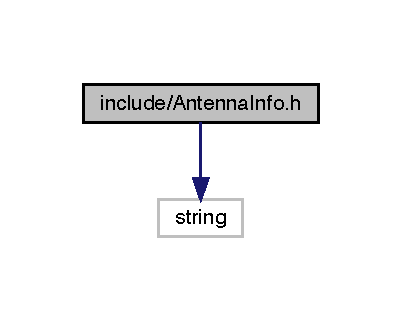
\includegraphics[width=193pt]{_antenna_info_8h__incl}
\end{center}
\end{figure}
This graph shows which files directly or indirectly include this file\+:
\nopagebreak
\begin{figure}[H]
\begin{center}
\leavevmode
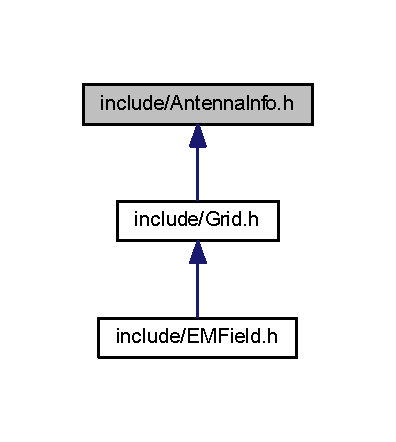
\includegraphics[width=193pt]{_antenna_info_8h__dep__incl}
\end{center}
\end{figure}
\subsection*{Classes}
\begin{DoxyCompactItemize}
\item 
class \mbox{\hyperlink{class_antenna_info}{Antenna\+Info}}
\end{DoxyCompactItemize}

\section{include/\+Antenna\+Type.h File Reference}
\label{_antenna_type_8h}\index{include/AntennaType.h@{include/AntennaType.h}}
\subsection*{Enumerations}
\begin{DoxyCompactItemize}
\item 
enum \textbf{ Antenna\+Type} \{ \textbf{ Antenna\+Type\+::\+O\+M\+N\+I\+D\+I\+R\+E\+C\+T\+I\+O\+N\+AL}, 
\textbf{ Antenna\+Type\+::\+D\+I\+R\+E\+C\+T\+I\+O\+N\+AL}
 \}
\end{DoxyCompactItemize}


\subsection{Enumeration Type Documentation}
\mbox{\label{_antenna_type_8h_a7b678b5cb9dedc607131200119d96b16}} 
\index{AntennaType.h@{AntennaType.h}!AntennaType@{AntennaType}}
\index{AntennaType@{AntennaType}!AntennaType.h@{AntennaType.h}}
\subsubsection{AntennaType}
{\footnotesize\ttfamily enum \textbf{ Antenna\+Type}\hspace{0.3cm}{\ttfamily [strong]}}

An enum class that is used to represent the type of an antenna. \begin{DoxyEnumFields}{Enumerator}
\raisebox{\heightof{T}}[0pt][0pt]{\index{OMNIDIRECTIONAL@{OMNIDIRECTIONAL}!AntennaType.h@{AntennaType.h}}\index{AntennaType.h@{AntennaType.h}!OMNIDIRECTIONAL@{OMNIDIRECTIONAL}}}\mbox{\label{_antenna_type_8h_a7b678b5cb9dedc607131200119d96b16a8ff57fa72952e98025e600a041b8b8de}} 
O\+M\+N\+I\+D\+I\+R\+E\+C\+T\+I\+O\+N\+AL&\\
\hline

\raisebox{\heightof{T}}[0pt][0pt]{\index{DIRECTIONAL@{DIRECTIONAL}!AntennaType.h@{AntennaType.h}}\index{AntennaType.h@{AntennaType.h}!DIRECTIONAL@{DIRECTIONAL}}}\mbox{\label{_antenna_type_8h_a7b678b5cb9dedc607131200119d96b16ab6f2249394a4def60a78b342dcc925b9}} 
D\+I\+R\+E\+C\+T\+I\+O\+N\+AL&\\
\hline

\end{DoxyEnumFields}


Definition at line 16 of file Antenna\+Type.\+h.


\hypertarget{_clock_8h}{}\section{include/\+Clock.h File Reference}
\label{_clock_8h}\index{include/Clock.h@{include/Clock.h}}
{\ttfamily \#include $<$chrono$>$}\newline
{\ttfamily \#include $<$ctime$>$}\newline
{\ttfamily \#include $<$time.\+h$>$}\newline
Include dependency graph for Clock.\+h\+:\nopagebreak
\begin{figure}[H]
\begin{center}
\leavevmode
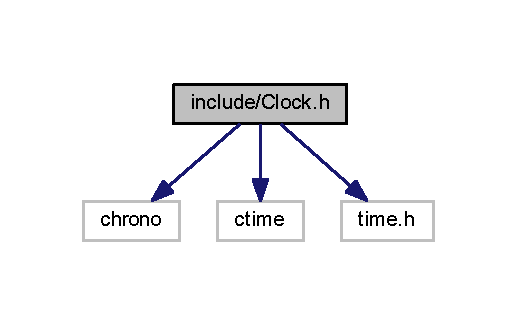
\includegraphics[width=246pt]{_clock_8h__incl}
\end{center}
\end{figure}
This graph shows which files directly or indirectly include this file\+:
\nopagebreak
\begin{figure}[H]
\begin{center}
\leavevmode
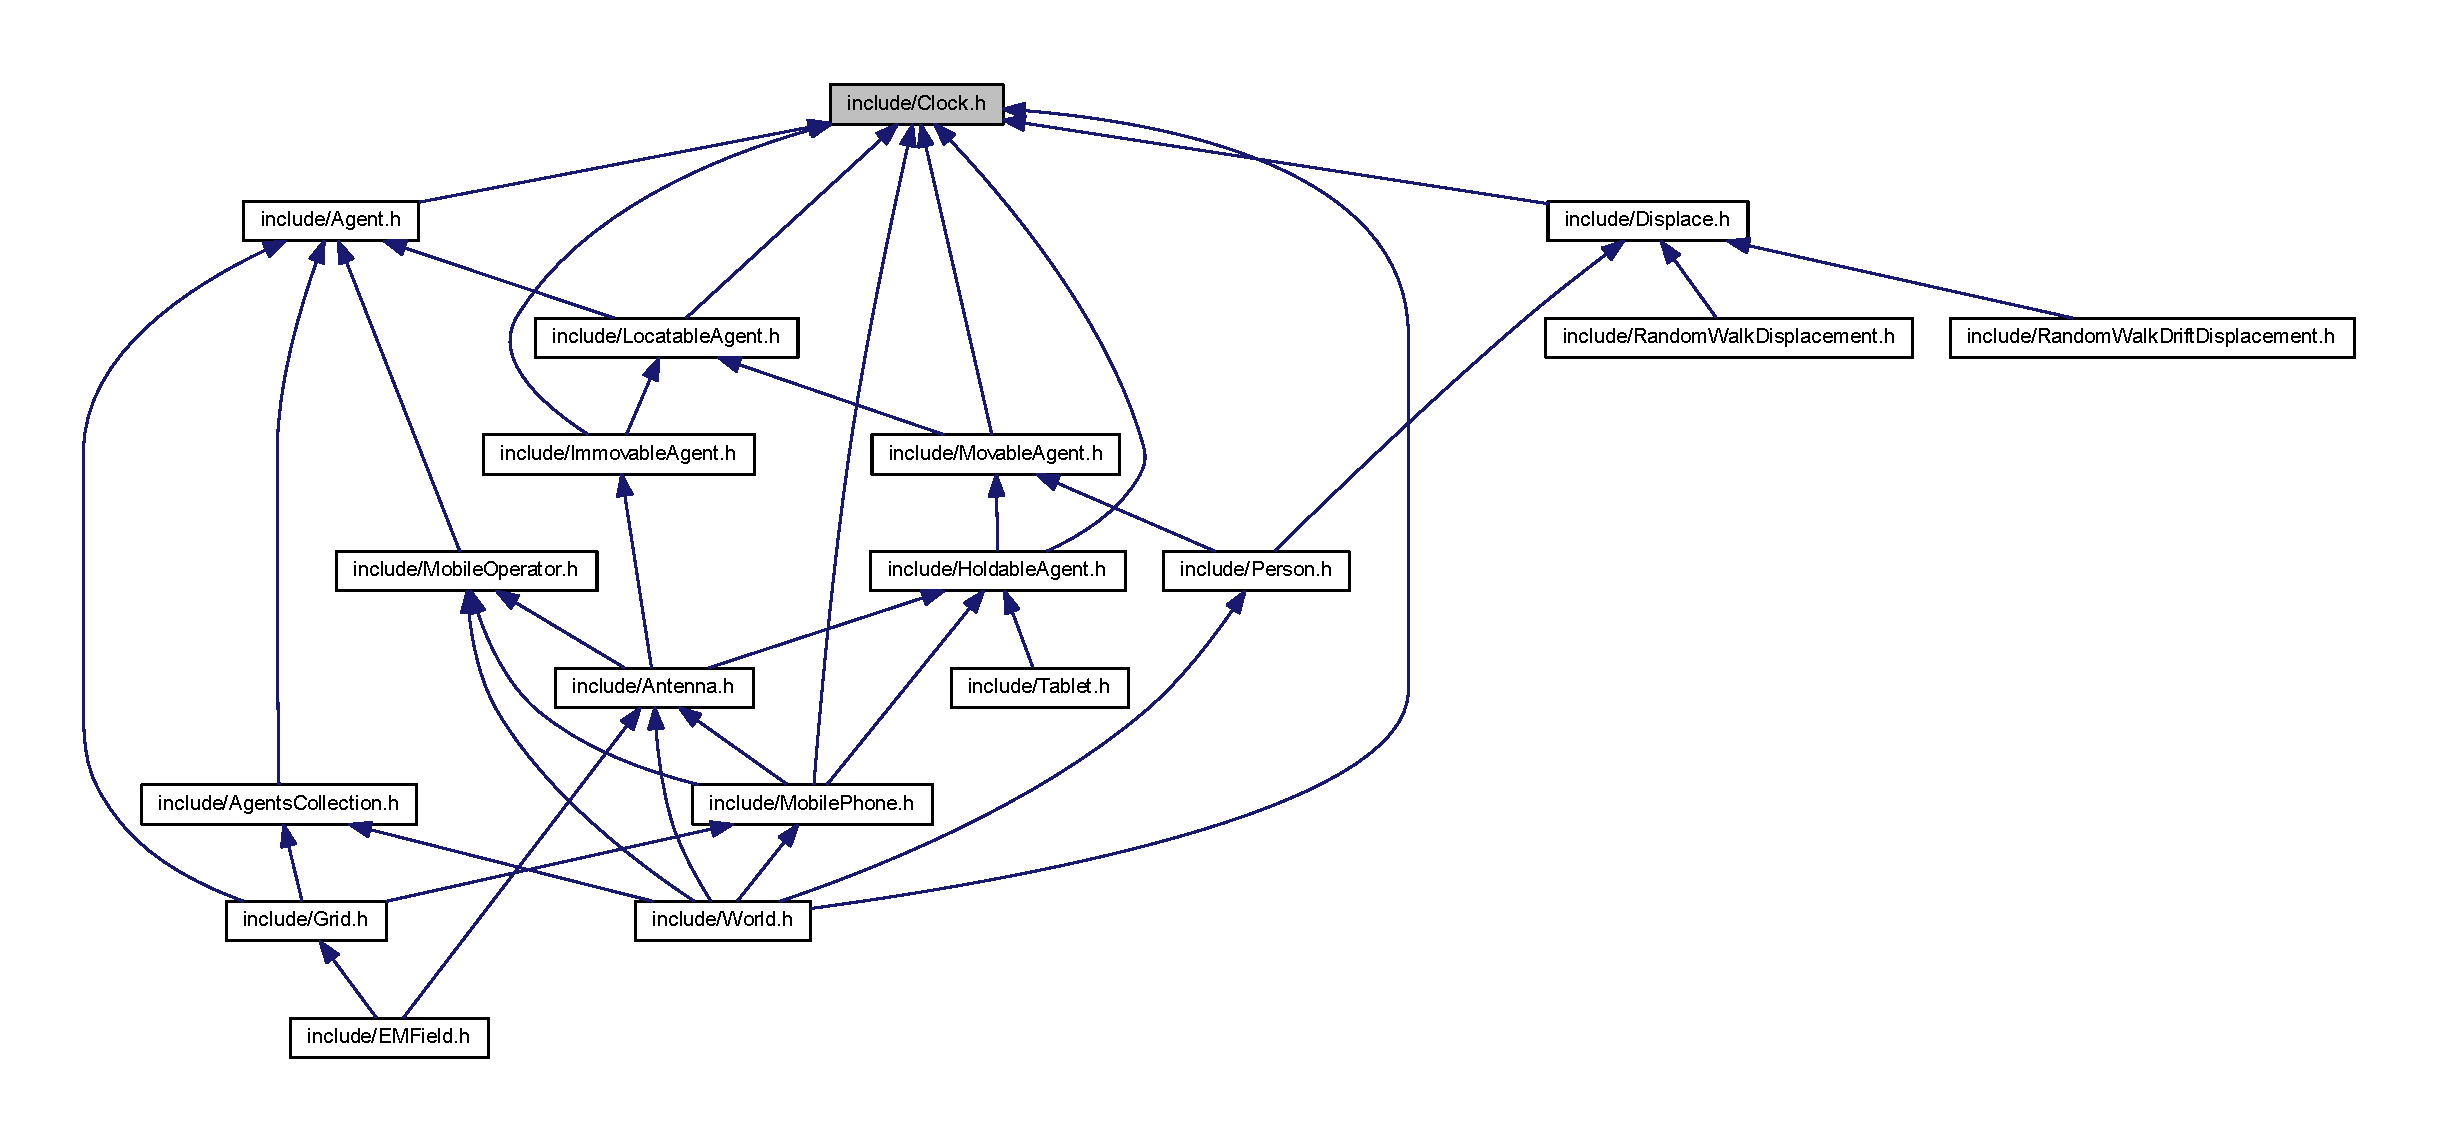
\includegraphics[width=350pt]{_clock_8h__dep__incl}
\end{center}
\end{figure}
\subsection*{Classes}
\begin{DoxyCompactItemize}
\item 
class \mbox{\hyperlink{class_clock}{Clock}}
\end{DoxyCompactItemize}

\section{include/\+Constants.h File Reference}
\label{_constants_8h}\index{include/Constants.h@{include/Constants.h}}
\subsection*{Classes}
\begin{DoxyCompactItemize}
\item 
class \textbf{ Constants}
\end{DoxyCompactItemize}

\section{include/\+C\+S\+Vparser.hpp File Reference}
\label{_c_s_vparser_8hpp}\index{include/CSVparser.hpp@{include/CSVparser.hpp}}
{\ttfamily \#include $<$stdexcept$>$}\newline
{\ttfamily \#include $<$string$>$}\newline
{\ttfamily \#include $<$vector$>$}\newline
{\ttfamily \#include $<$list$>$}\newline
{\ttfamily \#include $<$sstream$>$}\newline
\subsection*{Classes}
\begin{DoxyCompactItemize}
\item 
class \textbf{ Error}
\item 
class \textbf{ Row}
\item 
class \textbf{ Parser}
\end{DoxyCompactItemize}
\subsection*{Enumerations}
\begin{DoxyCompactItemize}
\item 
enum \textbf{ Data\+Type} \{ \textbf{ e\+F\+I\+LE} = 0, 
\textbf{ e\+P\+U\+RE} = 1
 \}
\end{DoxyCompactItemize}


\subsection{Enumeration Type Documentation}
\mbox{\label{_c_s_vparser_8hpp_ad8ed01ff3ff33333d8e19db4d2818bb6}} 
\index{CSVparser.hpp@{CSVparser.hpp}!DataType@{DataType}}
\index{DataType@{DataType}!CSVparser.hpp@{CSVparser.hpp}}
\subsubsection{DataType}
{\footnotesize\ttfamily enum \textbf{ Data\+Type}}

\begin{DoxyEnumFields}{Enumerator}
\raisebox{\heightof{T}}[0pt][0pt]{\index{eFILE@{eFILE}!CSVparser.hpp@{CSVparser.hpp}}\index{CSVparser.hpp@{CSVparser.hpp}!eFILE@{eFILE}}}\mbox{\label{_c_s_vparser_8hpp_ad8ed01ff3ff33333d8e19db4d2818bb6a99e2aefa5a03705fd10b8b72e081349f}} 
e\+F\+I\+LE&\\
\hline

\raisebox{\heightof{T}}[0pt][0pt]{\index{ePURE@{ePURE}!CSVparser.hpp@{CSVparser.hpp}}\index{CSVparser.hpp@{CSVparser.hpp}!ePURE@{ePURE}}}\mbox{\label{_c_s_vparser_8hpp_ad8ed01ff3ff33333d8e19db4d2818bb6aef7f347978c58a657566792291ec1e4b}} 
e\+P\+U\+RE&\\
\hline

\end{DoxyEnumFields}


Definition at line 53 of file C\+S\+Vparser.\+hpp.


\input{_displace_8h}
\hypertarget{_e_m_field_8h}{}\section{include/\+E\+M\+Field.h File Reference}
\label{_e_m_field_8h}\index{include/EMField.h@{include/EMField.h}}
{\ttfamily \#include $<$Antenna.\+h$>$}\newline
{\ttfamily \#include $<$Constants.\+h$>$}\newline
{\ttfamily \#include $<$Grid.\+h$>$}\newline
{\ttfamily \#include $<$utility$>$}\newline
{\ttfamily \#include $<$vector$>$}\newline
{\ttfamily \#include $<$map$>$}\newline
Include dependency graph for E\+M\+Field.\+h\+:\nopagebreak
\begin{figure}[H]
\begin{center}
\leavevmode
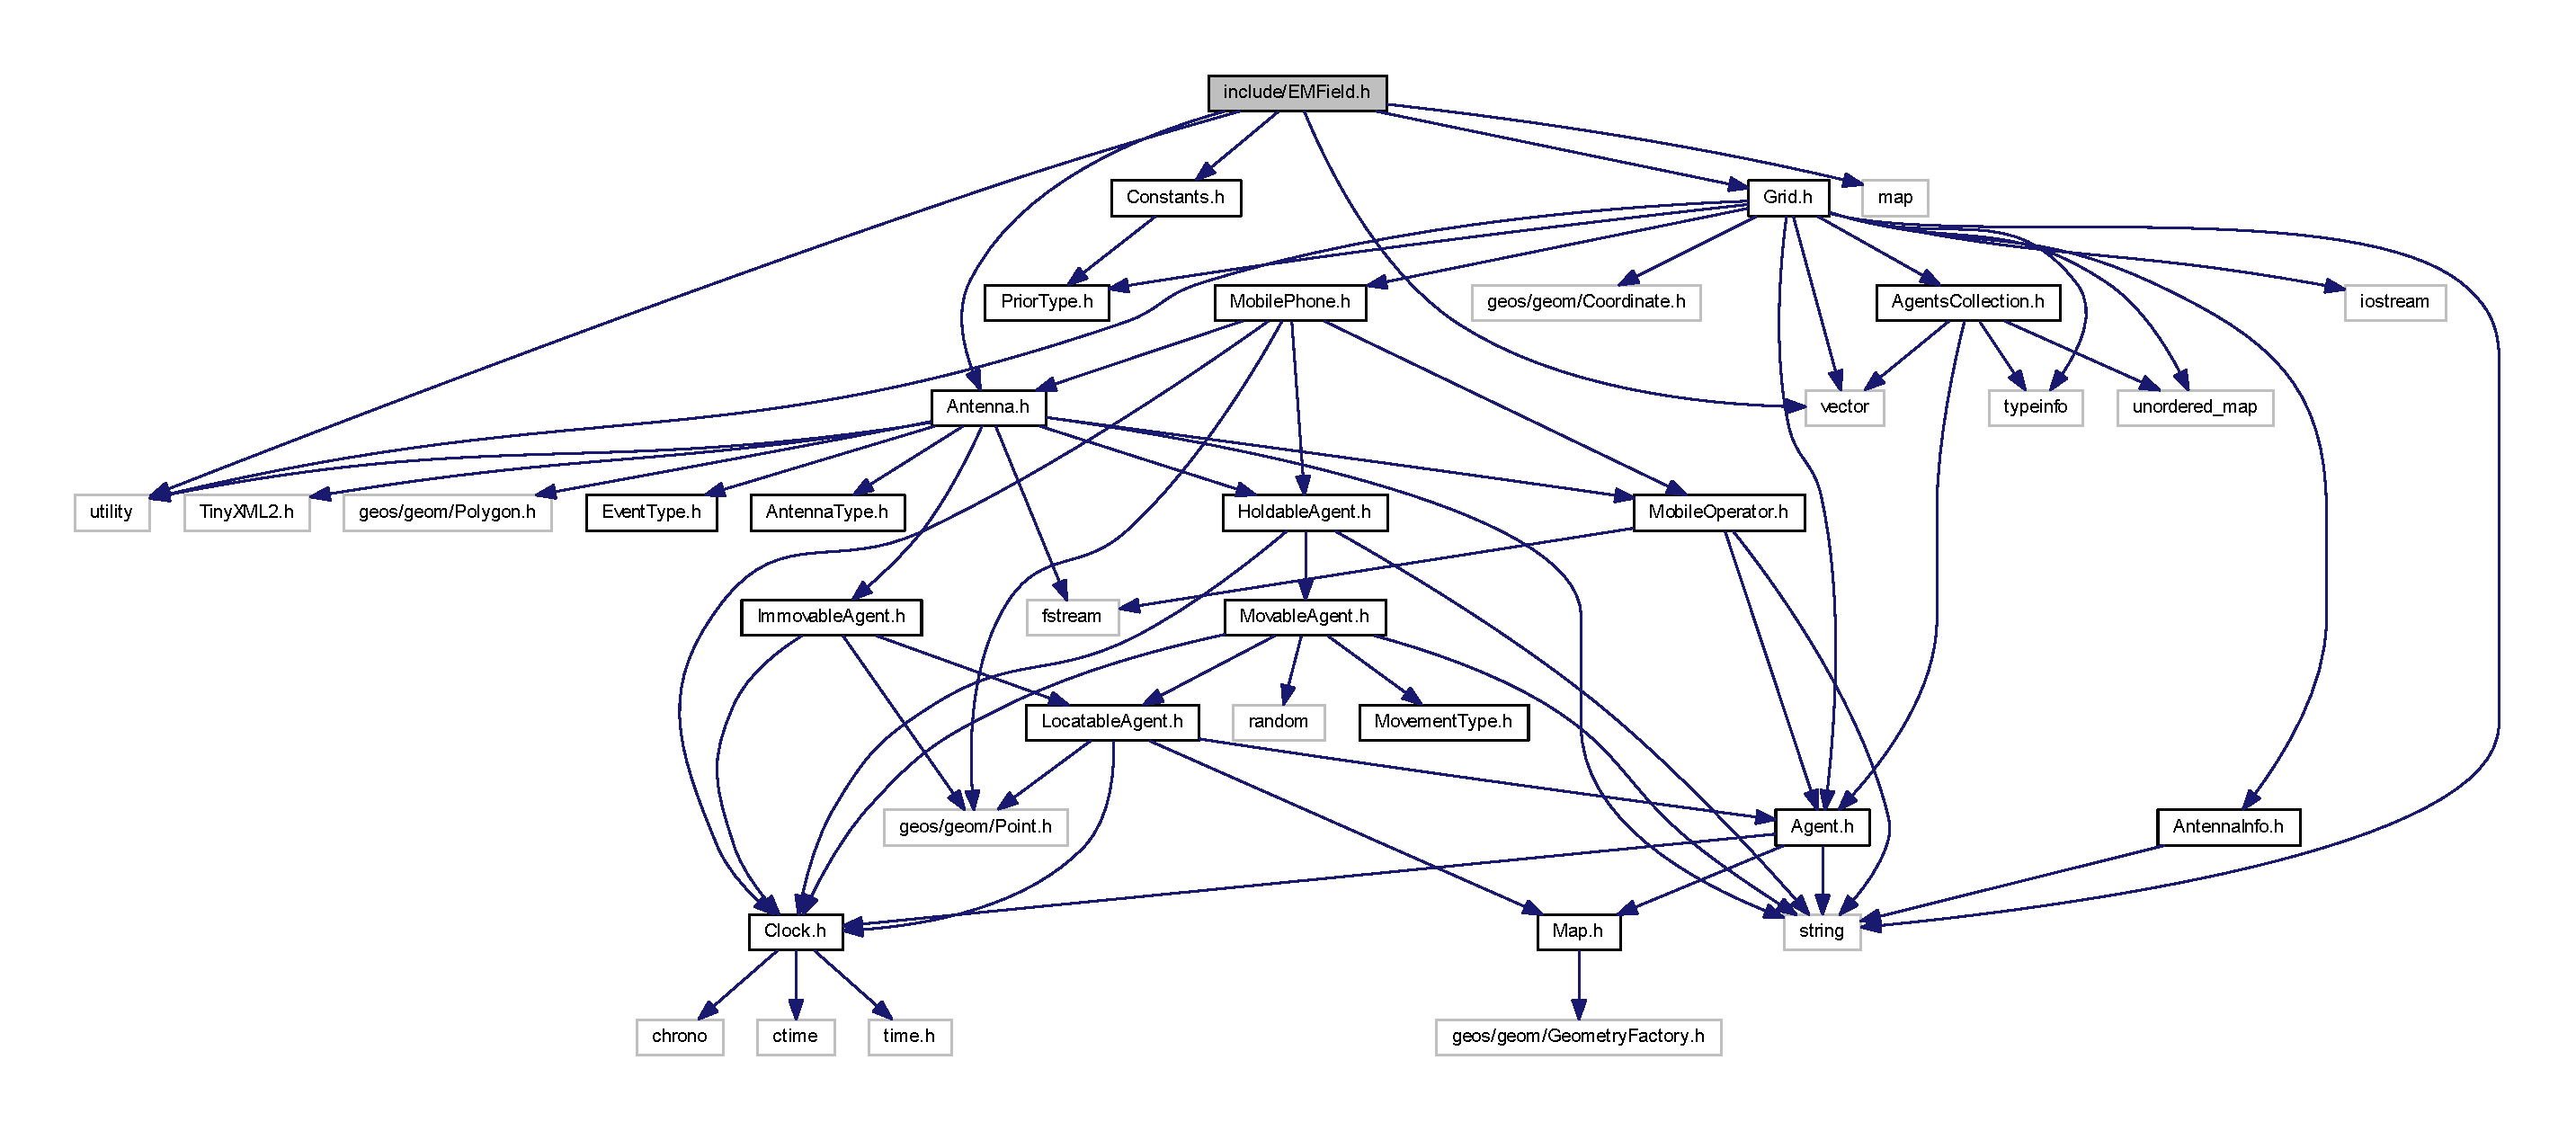
\includegraphics[width=350pt]{_e_m_field_8h__incl}
\end{center}
\end{figure}
\subsection*{Classes}
\begin{DoxyCompactItemize}
\item 
class \mbox{\hyperlink{class_e_m_field}{E\+M\+Field}}
\end{DoxyCompactItemize}

\hypertarget{_event_type_8h}{}\section{include/\+Event\+Type.h File Reference}
\label{_event_type_8h}\index{include/\+Event\+Type.\+h@{include/\+Event\+Type.\+h}}
This graph shows which files directly or indirectly include this file\+:\nopagebreak
\begin{figure}[H]
\begin{center}
\leavevmode
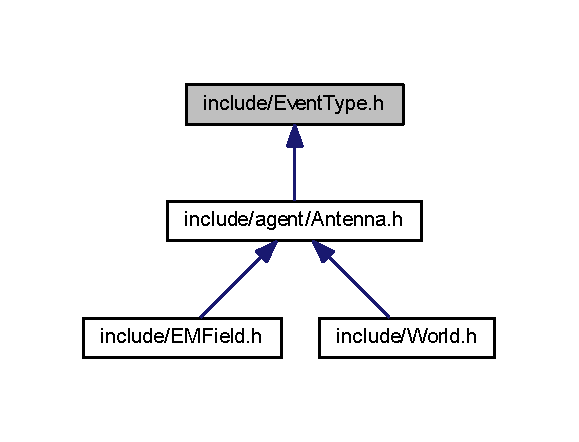
\includegraphics[width=306pt]{_event_type_8h__dep__incl}
\end{center}
\end{figure}
\subsection*{Enumerations}
\begin{DoxyCompactItemize}
\item 
enum \hyperlink{_event_type_8h_a2628ea8d12e8b2563c32f05dc7fff6fa}{Event\+Type} \{ \hyperlink{_event_type_8h_a2628ea8d12e8b2563c32f05dc7fff6faa9893a3a649e7100d87b1560bd8202ec2}{Event\+Type\+::\+A\+T\+T\+A\+C\+H\+\_\+\+D\+E\+V\+I\+CE}, 
\hyperlink{_event_type_8h_a2628ea8d12e8b2563c32f05dc7fff6faad4d5a45ac3a7a538879a9525fed18ddf}{Event\+Type\+::\+D\+E\+T\+A\+C\+H\+\_\+\+D\+E\+V\+I\+CE}, 
\hyperlink{_event_type_8h_a2628ea8d12e8b2563c32f05dc7fff6faaea76d50440d9cdc0ad1cac6ab9ac4f27}{Event\+Type\+::\+A\+L\+R\+E\+A\+D\+Y\+\_\+\+A\+T\+T\+A\+C\+H\+E\+D\+\_\+\+D\+E\+V\+I\+CE}, 
\hyperlink{_event_type_8h_a2628ea8d12e8b2563c32f05dc7fff6faa6ac0995df1d7ce888368dccf7af3e737}{Event\+Type\+::\+I\+N\+\_\+\+R\+A\+N\+G\+E\+\_\+\+N\+O\+T\+\_\+\+A\+T\+T\+A\+C\+H\+E\+D\+\_\+\+D\+E\+V\+I\+CE}
 \}
\end{DoxyCompactItemize}


\subsection{Enumeration Type Documentation}
\mbox{\Hypertarget{_event_type_8h_a2628ea8d12e8b2563c32f05dc7fff6fa}\label{_event_type_8h_a2628ea8d12e8b2563c32f05dc7fff6fa}} 
\index{Event\+Type.\+h@{Event\+Type.\+h}!Event\+Type@{Event\+Type}}
\index{Event\+Type@{Event\+Type}!Event\+Type.\+h@{Event\+Type.\+h}}
\subsubsection{\texorpdfstring{Event\+Type}{EventType}}
{\footnotesize\ttfamily enum \hyperlink{_event_type_8h_a2628ea8d12e8b2563c32f05dc7fff6fa}{Event\+Type}\hspace{0.3cm}{\ttfamily [strong]}}

This class is an enumeration of network events currently registered\+: A\+T\+T\+A\+C\+H\+\_\+\+D\+E\+V\+I\+CE -\/ means that an antenna connects a new mobile device. D\+E\+T\+A\+C\+H\+\_\+\+D\+E\+V\+I\+CE -\/ means that an antenna disconnects a mobile device, i.\+e. this mobile device is no longer connected to that antenna. A\+L\+R\+E\+A\+D\+Y\+\_\+\+A\+T\+T\+A\+C\+H\+E\+D\+\_\+\+D\+E\+V\+I\+CE -\/ means that an antenna is connected with a mobile device and that mobile was connected to the same antenna in the previous time step too. I\+N\+\_\+\+R\+A\+N\+G\+E\+\_\+\+N\+O\+T\+\_\+\+A\+T\+T\+A\+C\+H\+E\+D\+\_\+\+D\+E\+V\+I\+CE -\/ means that a mobile device tried to connect to an antenna, the antenna provided enough signal power/quality but the connection was not successful (for example antenna is at its maximum capacity and cannot connect any new devices). \begin{DoxyEnumFields}{Enumerator}
\raisebox{\heightof{T}}[0pt][0pt]{\index{A\+T\+T\+A\+C\+H\+\_\+\+D\+E\+V\+I\+CE@{A\+T\+T\+A\+C\+H\+\_\+\+D\+E\+V\+I\+CE}!Event\+Type.\+h@{Event\+Type.\+h}}\index{Event\+Type.\+h@{Event\+Type.\+h}!A\+T\+T\+A\+C\+H\+\_\+\+D\+E\+V\+I\+CE@{A\+T\+T\+A\+C\+H\+\_\+\+D\+E\+V\+I\+CE}}}\mbox{\Hypertarget{_event_type_8h_a2628ea8d12e8b2563c32f05dc7fff6faa9893a3a649e7100d87b1560bd8202ec2}\label{_event_type_8h_a2628ea8d12e8b2563c32f05dc7fff6faa9893a3a649e7100d87b1560bd8202ec2}} 
A\+T\+T\+A\+C\+H\+\_\+\+D\+E\+V\+I\+CE&\\
\hline

\raisebox{\heightof{T}}[0pt][0pt]{\index{D\+E\+T\+A\+C\+H\+\_\+\+D\+E\+V\+I\+CE@{D\+E\+T\+A\+C\+H\+\_\+\+D\+E\+V\+I\+CE}!Event\+Type.\+h@{Event\+Type.\+h}}\index{Event\+Type.\+h@{Event\+Type.\+h}!D\+E\+T\+A\+C\+H\+\_\+\+D\+E\+V\+I\+CE@{D\+E\+T\+A\+C\+H\+\_\+\+D\+E\+V\+I\+CE}}}\mbox{\Hypertarget{_event_type_8h_a2628ea8d12e8b2563c32f05dc7fff6faad4d5a45ac3a7a538879a9525fed18ddf}\label{_event_type_8h_a2628ea8d12e8b2563c32f05dc7fff6faad4d5a45ac3a7a538879a9525fed18ddf}} 
D\+E\+T\+A\+C\+H\+\_\+\+D\+E\+V\+I\+CE&\\
\hline

\raisebox{\heightof{T}}[0pt][0pt]{\index{A\+L\+R\+E\+A\+D\+Y\+\_\+\+A\+T\+T\+A\+C\+H\+E\+D\+\_\+\+D\+E\+V\+I\+CE@{A\+L\+R\+E\+A\+D\+Y\+\_\+\+A\+T\+T\+A\+C\+H\+E\+D\+\_\+\+D\+E\+V\+I\+CE}!Event\+Type.\+h@{Event\+Type.\+h}}\index{Event\+Type.\+h@{Event\+Type.\+h}!A\+L\+R\+E\+A\+D\+Y\+\_\+\+A\+T\+T\+A\+C\+H\+E\+D\+\_\+\+D\+E\+V\+I\+CE@{A\+L\+R\+E\+A\+D\+Y\+\_\+\+A\+T\+T\+A\+C\+H\+E\+D\+\_\+\+D\+E\+V\+I\+CE}}}\mbox{\Hypertarget{_event_type_8h_a2628ea8d12e8b2563c32f05dc7fff6faaea76d50440d9cdc0ad1cac6ab9ac4f27}\label{_event_type_8h_a2628ea8d12e8b2563c32f05dc7fff6faaea76d50440d9cdc0ad1cac6ab9ac4f27}} 
A\+L\+R\+E\+A\+D\+Y\+\_\+\+A\+T\+T\+A\+C\+H\+E\+D\+\_\+\+D\+E\+V\+I\+CE&\\
\hline

\raisebox{\heightof{T}}[0pt][0pt]{\index{I\+N\+\_\+\+R\+A\+N\+G\+E\+\_\+\+N\+O\+T\+\_\+\+A\+T\+T\+A\+C\+H\+E\+D\+\_\+\+D\+E\+V\+I\+CE@{I\+N\+\_\+\+R\+A\+N\+G\+E\+\_\+\+N\+O\+T\+\_\+\+A\+T\+T\+A\+C\+H\+E\+D\+\_\+\+D\+E\+V\+I\+CE}!Event\+Type.\+h@{Event\+Type.\+h}}\index{Event\+Type.\+h@{Event\+Type.\+h}!I\+N\+\_\+\+R\+A\+N\+G\+E\+\_\+\+N\+O\+T\+\_\+\+A\+T\+T\+A\+C\+H\+E\+D\+\_\+\+D\+E\+V\+I\+CE@{I\+N\+\_\+\+R\+A\+N\+G\+E\+\_\+\+N\+O\+T\+\_\+\+A\+T\+T\+A\+C\+H\+E\+D\+\_\+\+D\+E\+V\+I\+CE}}}\mbox{\Hypertarget{_event_type_8h_a2628ea8d12e8b2563c32f05dc7fff6faa6ac0995df1d7ce888368dccf7af3e737}\label{_event_type_8h_a2628ea8d12e8b2563c32f05dc7fff6faa6ac0995df1d7ce888368dccf7af3e737}} 
I\+N\+\_\+\+R\+A\+N\+G\+E\+\_\+\+N\+O\+T\+\_\+\+A\+T\+T\+A\+C\+H\+E\+D\+\_\+\+D\+E\+V\+I\+CE&\\
\hline

\end{DoxyEnumFields}

\hypertarget{_grid_8h}{}\section{include/map/\+Grid.h File Reference}
\label{_grid_8h}\index{include/map/\+Grid.\+h@{include/map/\+Grid.\+h}}
{\ttfamily \#include $<$string$>$}\newline
{\ttfamily \#include $<$iostream$>$}\newline
{\ttfamily \#include $<$geos/geom/\+Coordinate.\+h$>$}\newline
{\ttfamily \#include $<$geos/geom/\+Point.\+h$>$}\newline
Include dependency graph for Grid.\+h\+:
\nopagebreak
\begin{figure}[H]
\begin{center}
\leavevmode
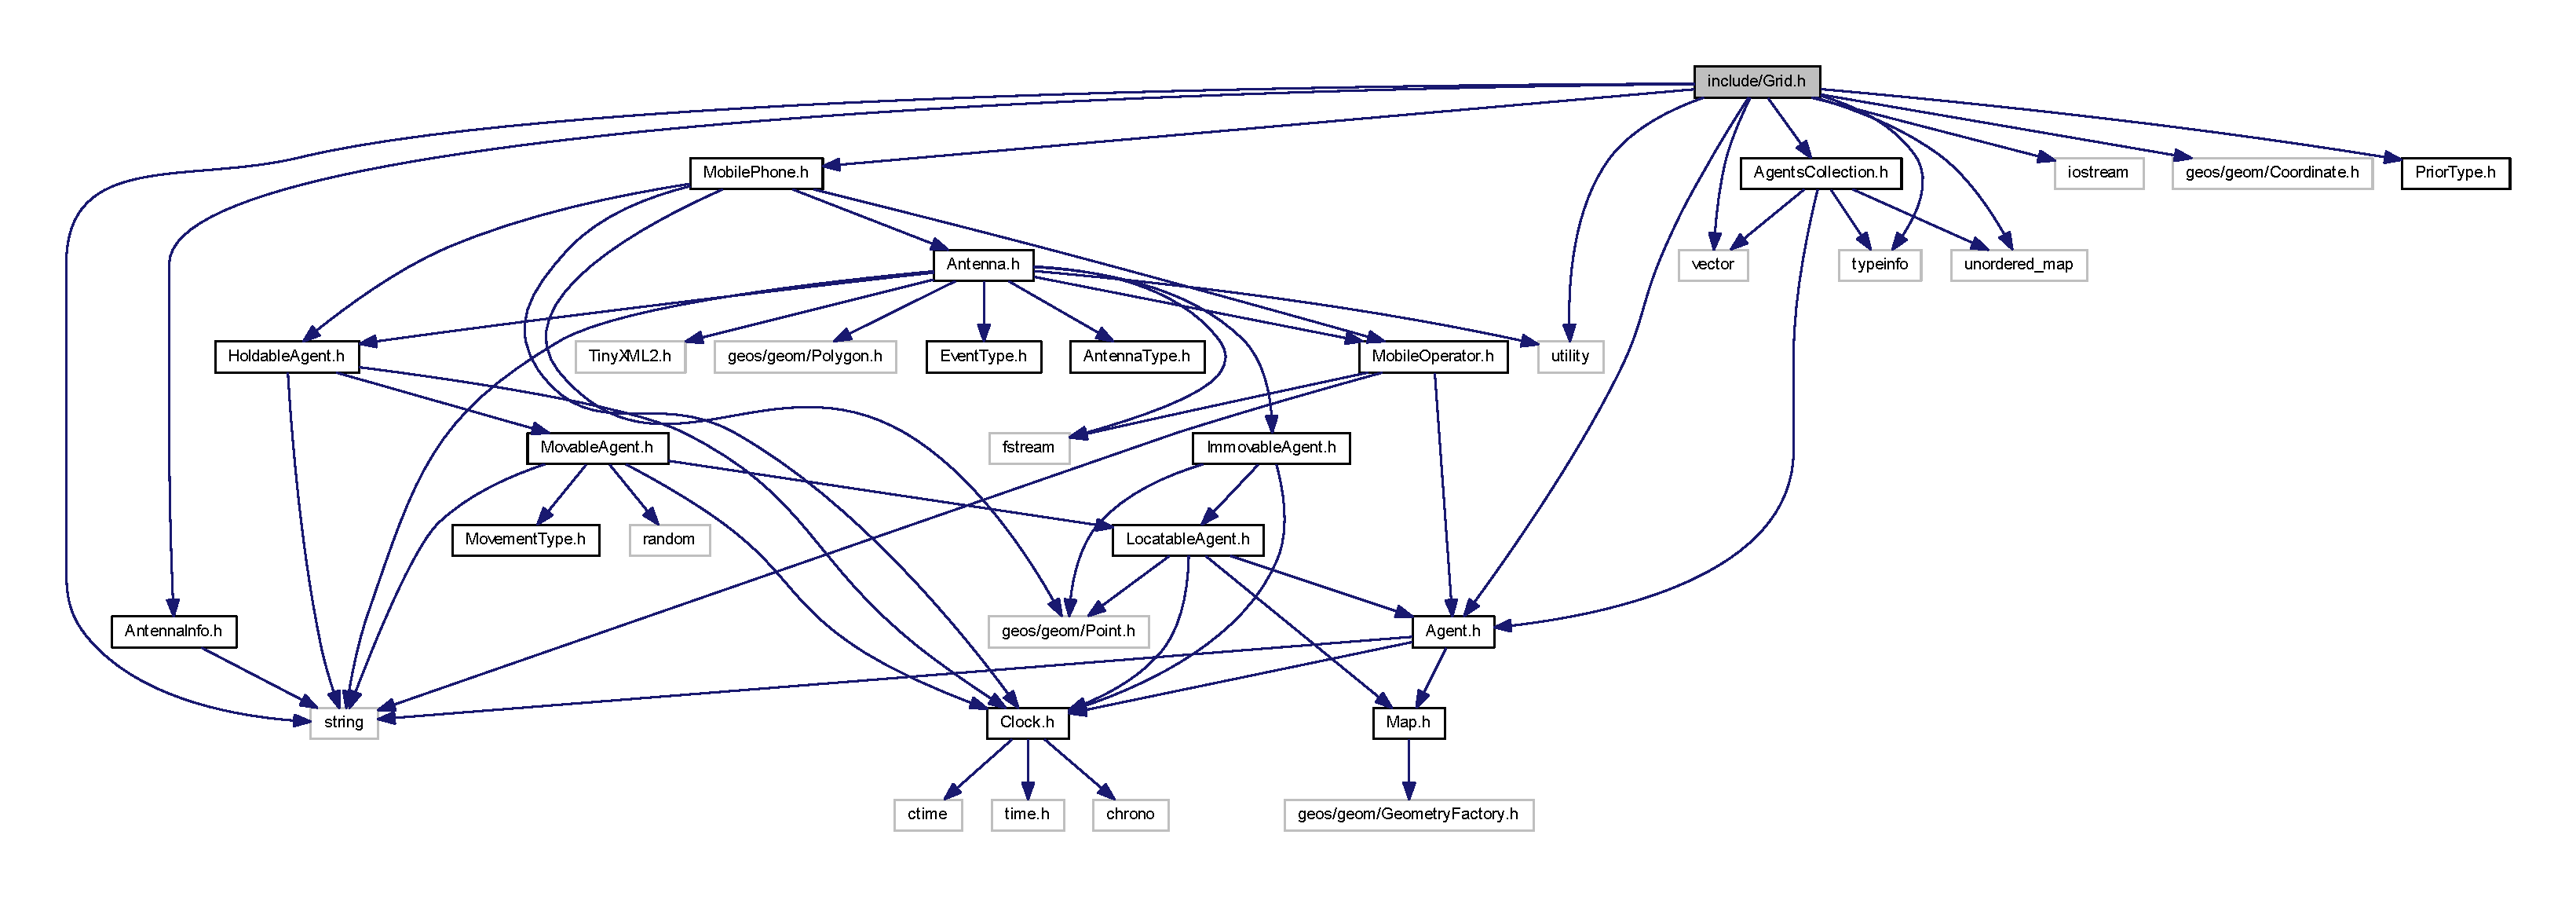
\includegraphics[width=350pt]{_grid_8h__incl}
\end{center}
\end{figure}
This graph shows which files directly or indirectly include this file\+:
\nopagebreak
\begin{figure}[H]
\begin{center}
\leavevmode
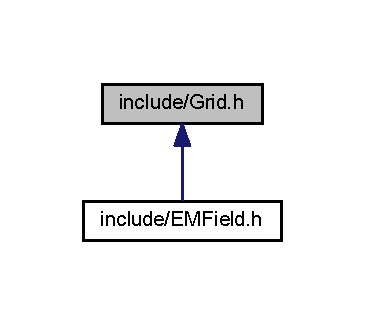
\includegraphics[width=350pt]{_grid_8h__dep__incl}
\end{center}
\end{figure}
\subsection*{Classes}
\begin{DoxyCompactItemize}
\item 
class \hyperlink{class_grid}{Grid}
\end{DoxyCompactItemize}

\section{include/\+Holdable\+Agent.h File Reference}
\label{_holdable_agent_8h}\index{include/HoldableAgent.h@{include/HoldableAgent.h}}
{\ttfamily \#include $<$Movable\+Agent.\+h$>$}\newline
{\ttfamily \#include $<$Clock.\+h$>$}\newline
{\ttfamily \#include $<$string$>$}\newline
\subsection*{Classes}
\begin{DoxyCompactItemize}
\item 
class \textbf{ Holdable\+Agent}
\end{DoxyCompactItemize}

\hypertarget{_i_d_generator_8h}{}\section{include/\+I\+D\+Generator.h File Reference}
\label{_i_d_generator_8h}\index{include/\+I\+D\+Generator.\+h@{include/\+I\+D\+Generator.\+h}}
\subsection*{Classes}
\begin{DoxyCompactItemize}
\item 
class \hyperlink{class_i_d_generator}{I\+D\+Generator}
\end{DoxyCompactItemize}

\hypertarget{_immovable_agent_8h}{}\section{include/\+Immovable\+Agent.h File Reference}
\label{_immovable_agent_8h}\index{include/ImmovableAgent.h@{include/ImmovableAgent.h}}
{\ttfamily \#include \char`\"{}Locatable\+Agent.\+h\char`\"{}}\newline
{\ttfamily \#include $<$Clock.\+h$>$}\newline
{\ttfamily \#include $<$geos/geom/\+Point.\+h$>$}\newline
Include dependency graph for Immovable\+Agent.\+h\+:\nopagebreak
\begin{figure}[H]
\begin{center}
\leavevmode
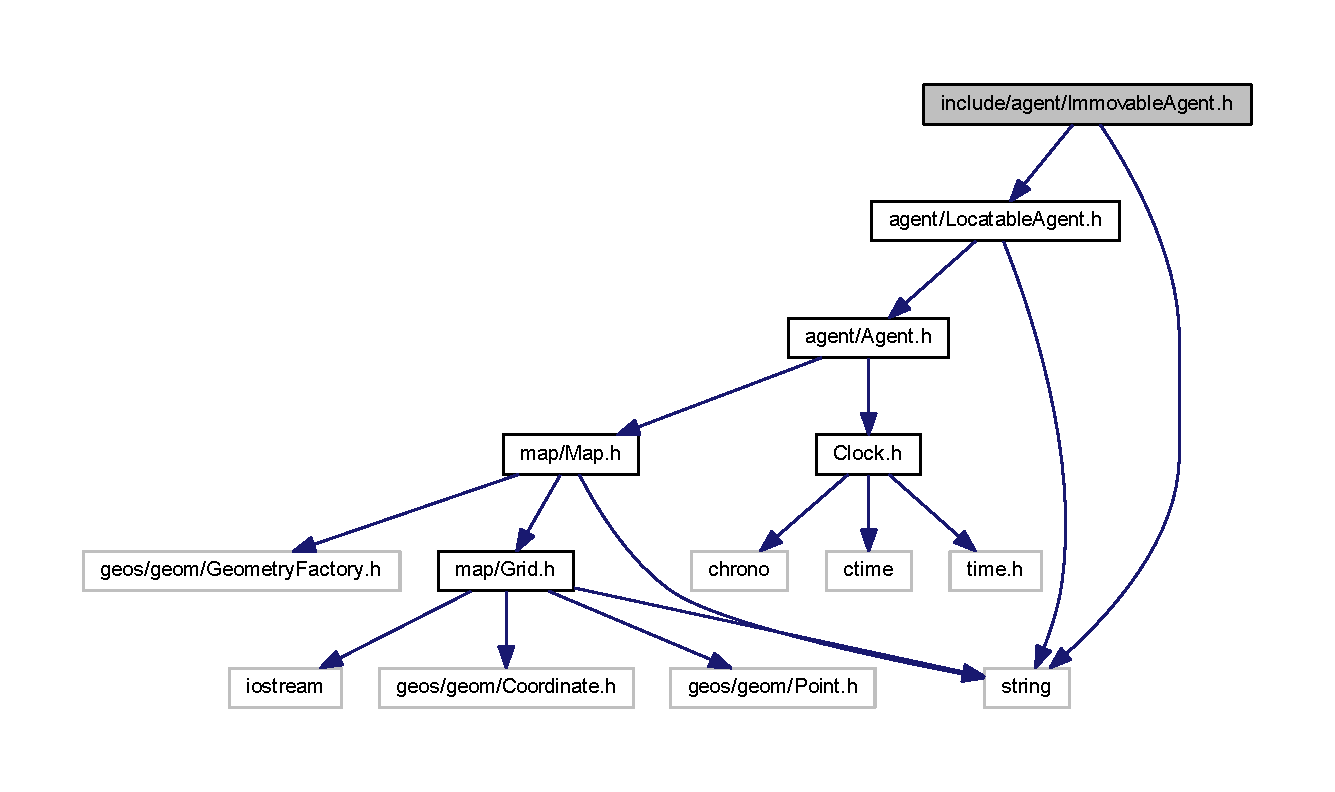
\includegraphics[width=350pt]{_immovable_agent_8h__incl}
\end{center}
\end{figure}
This graph shows which files directly or indirectly include this file\+:\nopagebreak
\begin{figure}[H]
\begin{center}
\leavevmode
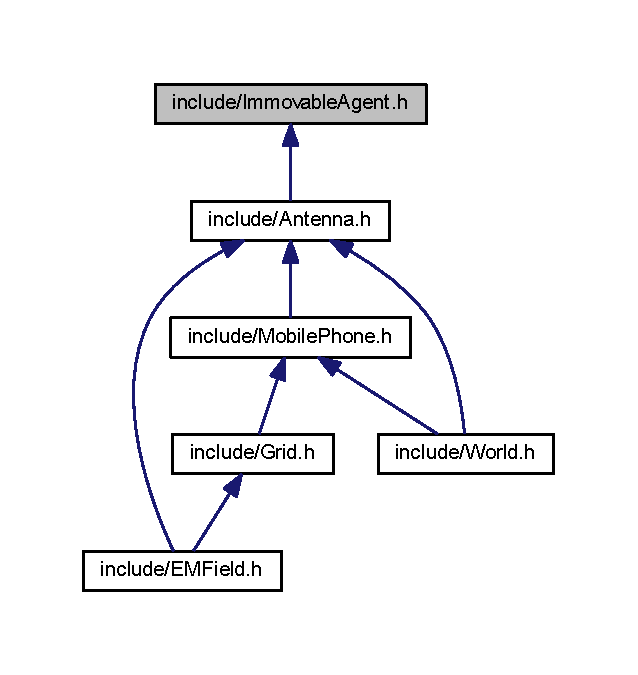
\includegraphics[width=309pt]{_immovable_agent_8h__dep__incl}
\end{center}
\end{figure}
\subsection*{Classes}
\begin{DoxyCompactItemize}
\item 
class \mbox{\hyperlink{class_immovable_agent}{Immovable\+Agent}}
\end{DoxyCompactItemize}

\section{include/\+Input\+Parser.h File Reference}
\label{_input_parser_8h}\index{include/InputParser.h@{include/InputParser.h}}
{\ttfamily \#include $<$string$>$}\newline
{\ttfamily \#include $<$vector$>$}\newline
\subsection*{Classes}
\begin{DoxyCompactItemize}
\item 
class \textbf{ Input\+Parser}
\end{DoxyCompactItemize}

\hypertarget{_locatable_agent_8h}{}\section{include/agent/\+Locatable\+Agent.h File Reference}
\label{_locatable_agent_8h}\index{include/agent/\+Locatable\+Agent.\+h@{include/agent/\+Locatable\+Agent.\+h}}
{\ttfamily \#include $<$agent/\+Agent.\+h$>$}\newline
{\ttfamily \#include $<$string$>$}\newline
Include dependency graph for Locatable\+Agent.\+h\+:
\nopagebreak
\begin{figure}[H]
\begin{center}
\leavevmode
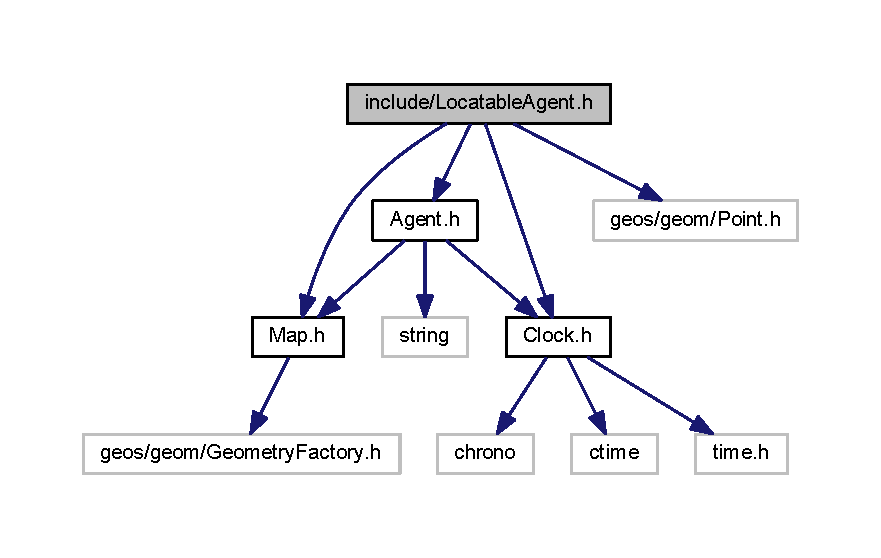
\includegraphics[width=350pt]{_locatable_agent_8h__incl}
\end{center}
\end{figure}
This graph shows which files directly or indirectly include this file\+:
\nopagebreak
\begin{figure}[H]
\begin{center}
\leavevmode
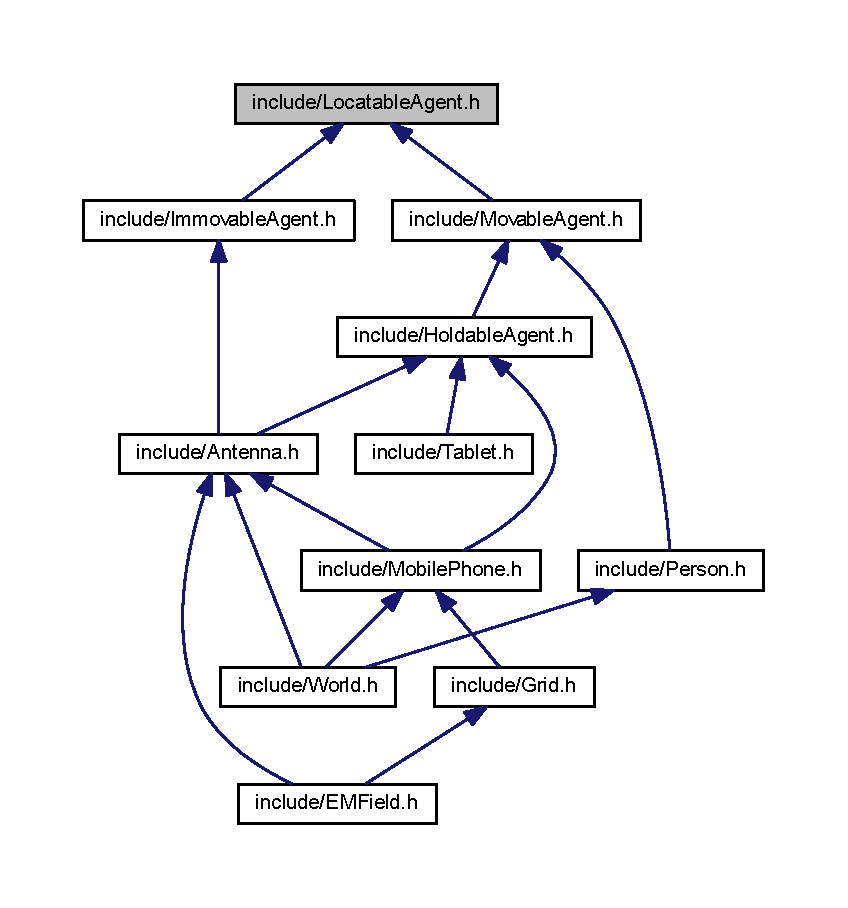
\includegraphics[width=350pt]{_locatable_agent_8h__dep__incl}
\end{center}
\end{figure}
\subsection*{Classes}
\begin{DoxyCompactItemize}
\item 
class \hyperlink{class_locatable_agent}{Locatable\+Agent}
\end{DoxyCompactItemize}

\hypertarget{_map_8h}{}\section{include/\+Map.h File Reference}
\label{_map_8h}\index{include/Map.h@{include/Map.h}}
{\ttfamily \#include $<$geos/geom/\+Geometry\+Factory.\+h$>$}\newline
Include dependency graph for Map.\+h\+:
\nopagebreak
\begin{figure}[H]
\begin{center}
\leavevmode
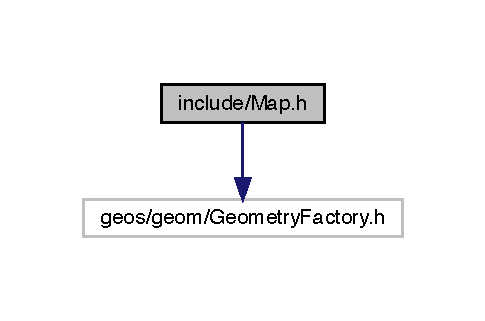
\includegraphics[width=233pt]{_map_8h__incl}
\end{center}
\end{figure}
This graph shows which files directly or indirectly include this file\+:
\nopagebreak
\begin{figure}[H]
\begin{center}
\leavevmode
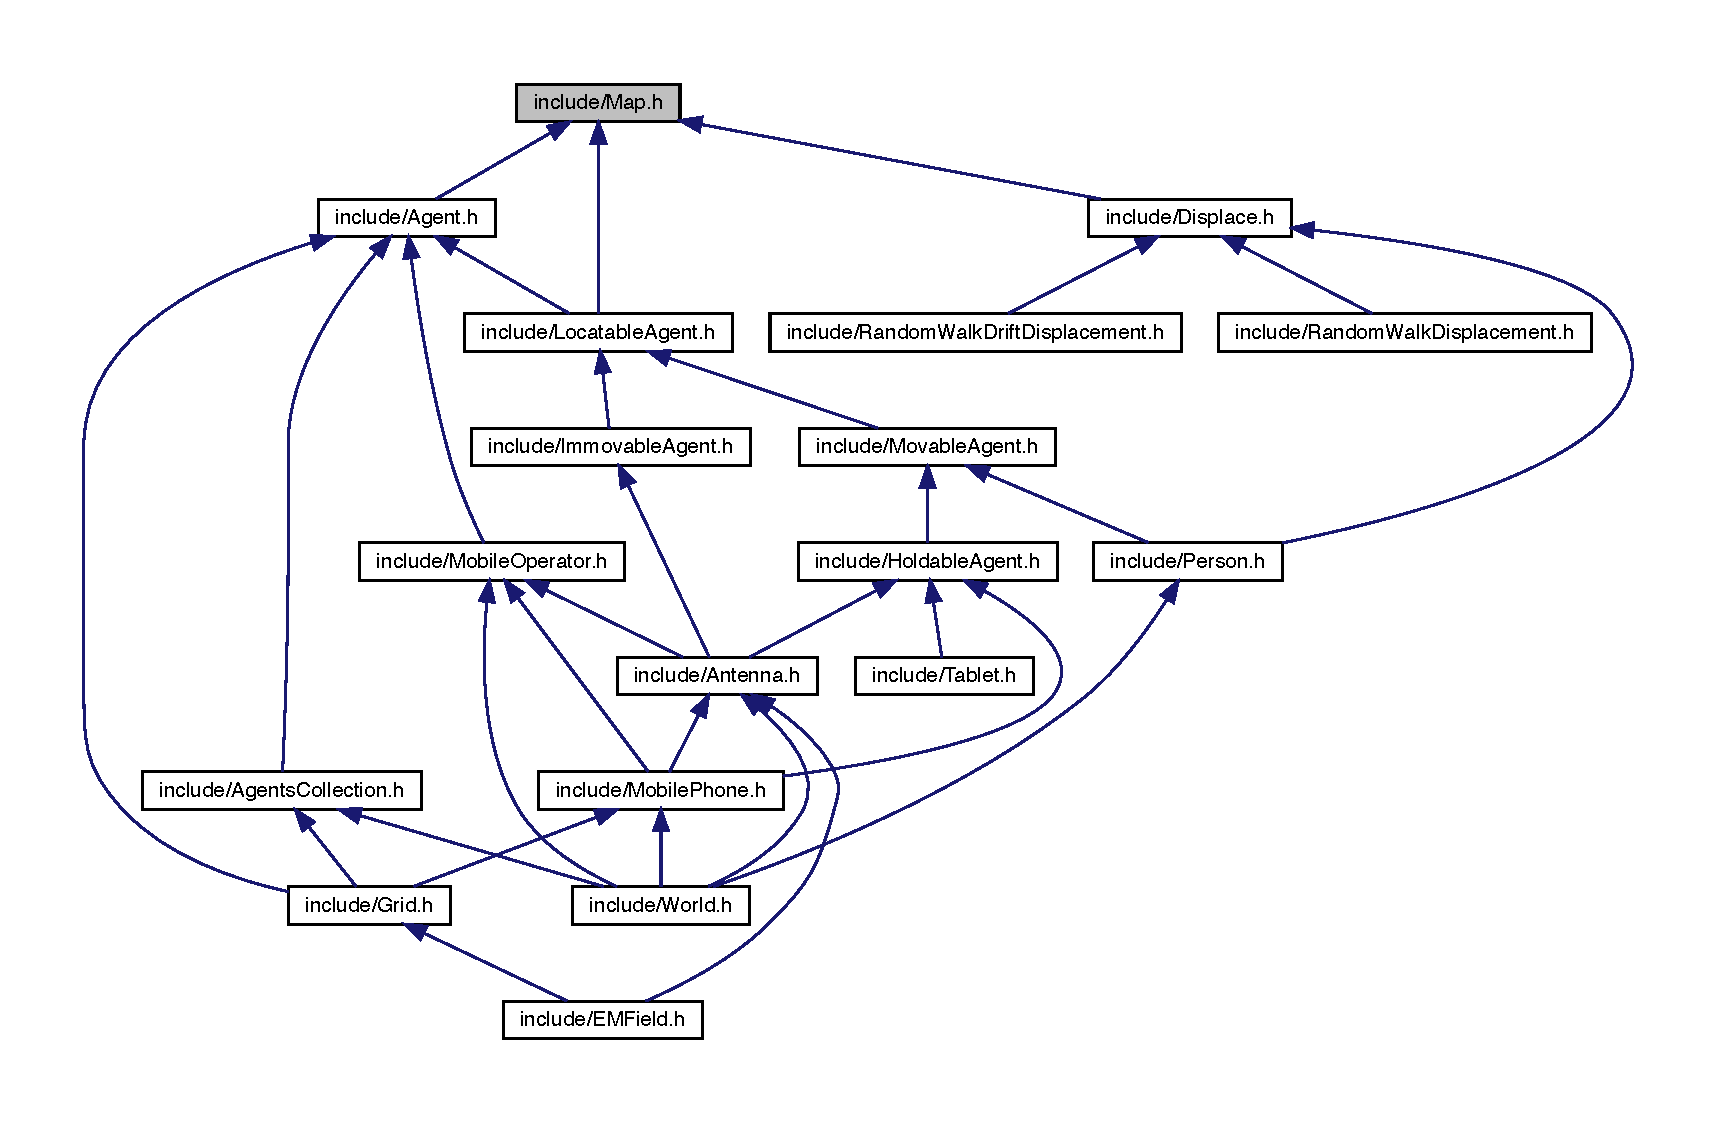
\includegraphics[width=350pt]{_map_8h__dep__incl}
\end{center}
\end{figure}
\subsection*{Classes}
\begin{DoxyCompactItemize}
\item 
class \mbox{\hyperlink{class_map}{Map}}
\end{DoxyCompactItemize}

\hypertarget{_mobile_operator_8h}{}\section{include/agent/\+Mobile\+Operator.h File Reference}
\label{_mobile_operator_8h}\index{include/agent/\+Mobile\+Operator.\+h@{include/agent/\+Mobile\+Operator.\+h}}
{\ttfamily \#include $<$agent/\+Agent.\+h$>$}\newline
{\ttfamily \#include $<$fstream$>$}\newline
{\ttfamily \#include $<$string$>$}\newline
Include dependency graph for Mobile\+Operator.\+h\+:
\nopagebreak
\begin{figure}[H]
\begin{center}
\leavevmode
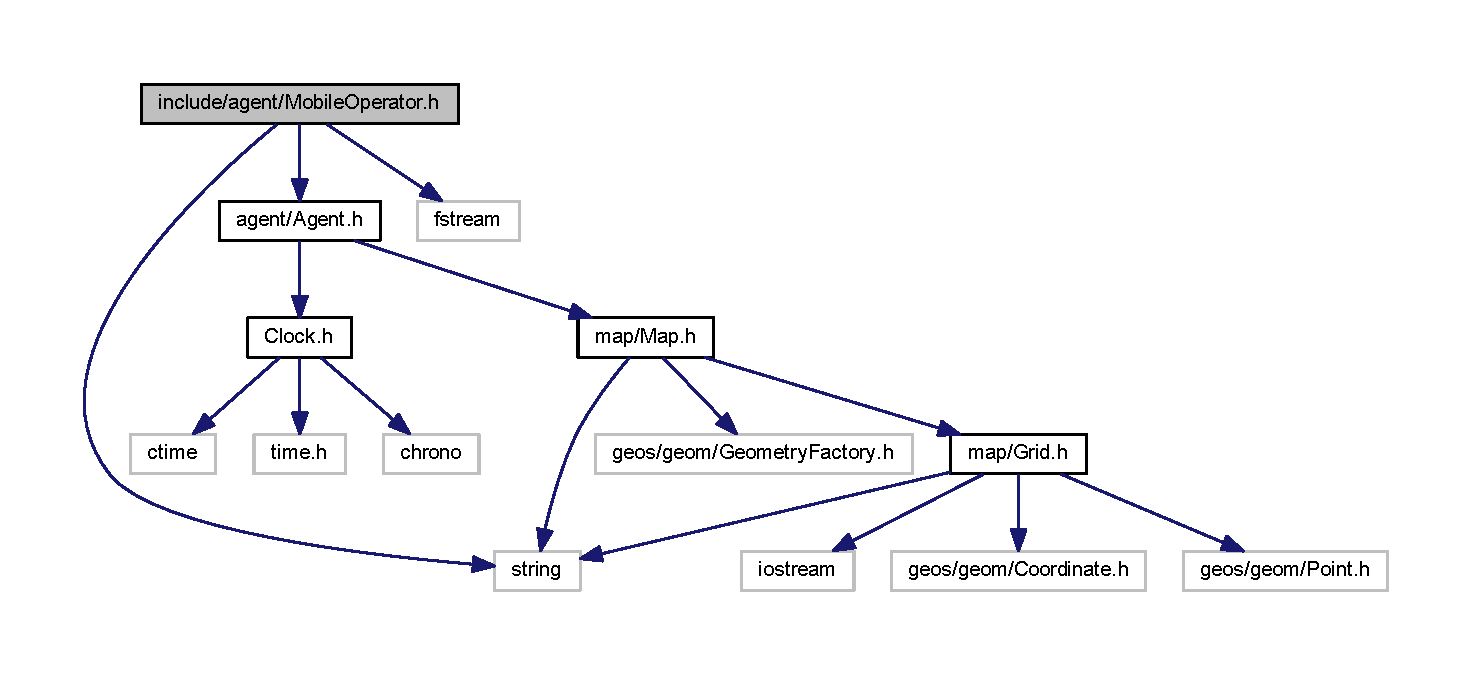
\includegraphics[width=350pt]{_mobile_operator_8h__incl}
\end{center}
\end{figure}
This graph shows which files directly or indirectly include this file\+:
\nopagebreak
\begin{figure}[H]
\begin{center}
\leavevmode
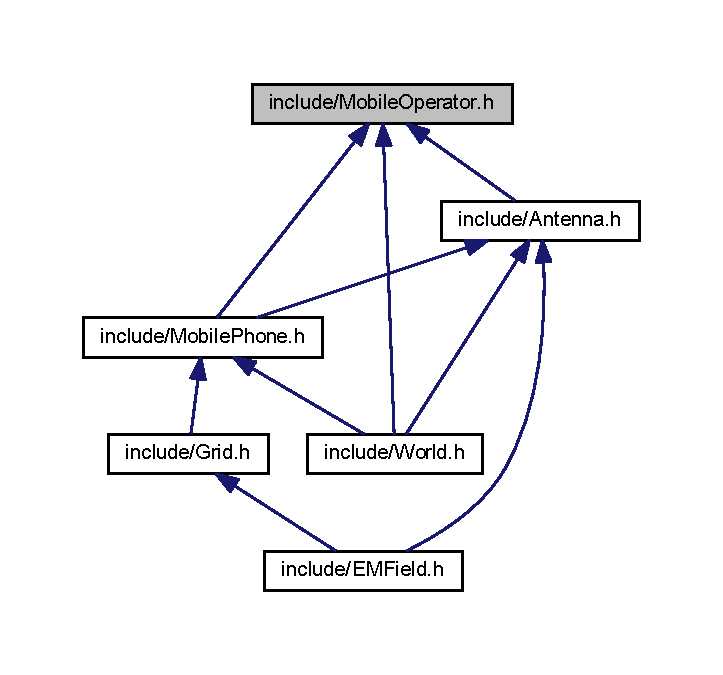
\includegraphics[width=278pt]{_mobile_operator_8h__dep__incl}
\end{center}
\end{figure}
\subsection*{Classes}
\begin{DoxyCompactItemize}
\item 
class \hyperlink{class_mobile_operator}{Mobile\+Operator}
\end{DoxyCompactItemize}

\section{include/\+Mobile\+Phone.h File Reference}
\label{_mobile_phone_8h}\index{include/\+Mobile\+Phone.\+h@{include/\+Mobile\+Phone.\+h}}
{\ttfamily \#include $<$Holdable\+Agent.\+h$>$}\newline
{\ttfamily \#include $<$Antenna.\+h$>$}\newline
{\ttfamily \#include $<$Clock.\+h$>$}\newline
{\ttfamily \#include $<$geos/geom/\+Point.\+h$>$}\newline
Include dependency graph for Mobile\+Phone.\+h\+:
% FIG 0
This graph shows which files directly or indirectly include this file\+:
% FIG 1
\subsection*{Classes}
\begin{DoxyCompactItemize}
\item 
class \textbf{ Mobile\+Phone}
\end{DoxyCompactItemize}

\hypertarget{_movable_agent_8h}{}\section{include/\+Movable\+Agent.h File Reference}
\label{_movable_agent_8h}\index{include/MovableAgent.h@{include/MovableAgent.h}}
{\ttfamily \#include $<$Locatable\+Agent.\+h$>$}\newline
{\ttfamily \#include $<$Clock.\+h$>$}\newline
{\ttfamily \#include $<$random$>$}\newline
{\ttfamily \#include $<$Movement\+Type.\+h$>$}\newline
{\ttfamily \#include $<$string$>$}\newline
Include dependency graph for Movable\+Agent.\+h\+:
\nopagebreak
\begin{figure}[H]
\begin{center}
\leavevmode
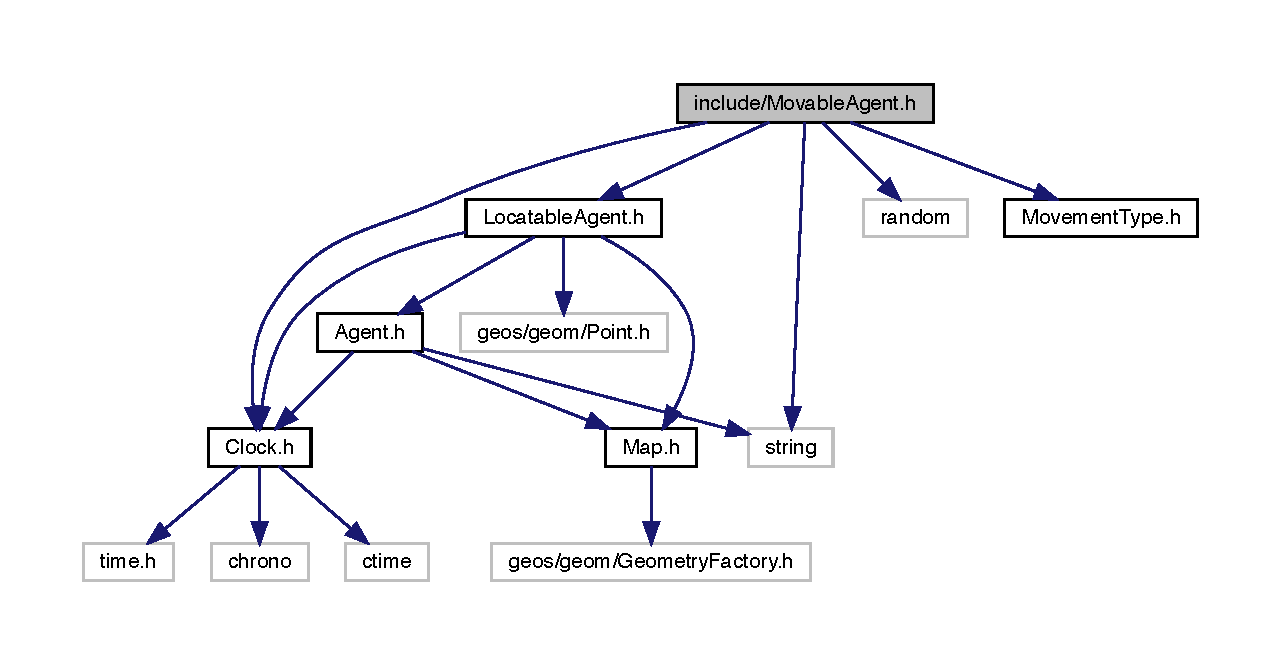
\includegraphics[width=350pt]{_movable_agent_8h__incl}
\end{center}
\end{figure}
This graph shows which files directly or indirectly include this file\+:
\nopagebreak
\begin{figure}[H]
\begin{center}
\leavevmode
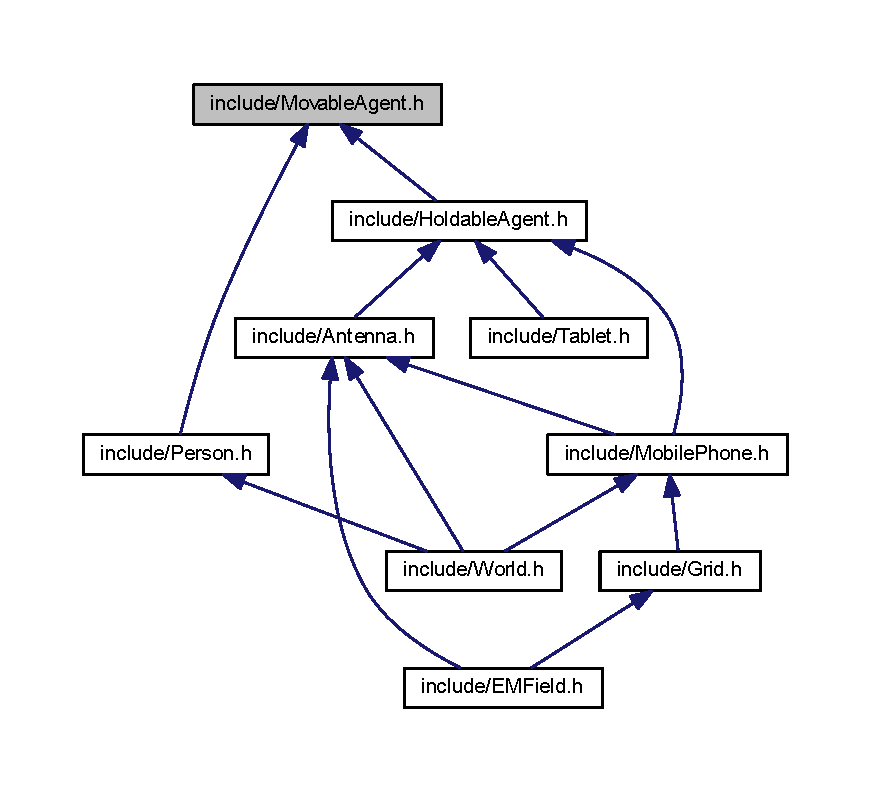
\includegraphics[width=350pt]{_movable_agent_8h__dep__incl}
\end{center}
\end{figure}
\subsection*{Classes}
\begin{DoxyCompactItemize}
\item 
class \mbox{\hyperlink{class_movable_agent}{Movable\+Agent}}
\end{DoxyCompactItemize}

\hypertarget{_movement_type_8h}{}\section{include/\+Movement\+Type.h File Reference}
\label{_movement_type_8h}\index{include/MovementType.h@{include/MovementType.h}}
This graph shows which files directly or indirectly include this file\+:\nopagebreak
\begin{figure}[H]
\begin{center}
\leavevmode
\includegraphics[width=350pt]{_movement_type_8h__dep__incl}
\end{center}
\end{figure}
\subsection*{Enumerations}
\begin{DoxyCompactItemize}
\item 
enum \mbox{\hyperlink{_movement_type_8h_a8a93b61bc797a7d1907f42796a252493}{Movement\+Type}} \{ \mbox{\hyperlink{_movement_type_8h_a8a93b61bc797a7d1907f42796a252493a1260a39bdcc19395a0085be09746f9d0}{Movement\+Type\+::\+R\+A\+N\+D\+O\+M\+\_\+\+W\+A\+L\+K\+\_\+\+C\+L\+O\+S\+E\+D\+\_\+\+M\+AP}}, 
\mbox{\hyperlink{_movement_type_8h_a8a93b61bc797a7d1907f42796a252493a19d5a14b0e46bf765f243b7e2b7b8810}{Movement\+Type\+::\+R\+A\+N\+D\+O\+M\+\_\+\+W\+A\+L\+K\+\_\+\+C\+L\+O\+S\+E\+D\+\_\+\+M\+A\+P\+\_\+\+W\+I\+T\+H\+\_\+\+D\+R\+I\+FT}}, 
\mbox{\hyperlink{_movement_type_8h_a8a93b61bc797a7d1907f42796a252493a696b031073e74bf2cb98e5ef201d4aa3}{Movement\+Type\+::\+U\+N\+K\+N\+O\+WN}}
 \}
\end{DoxyCompactItemize}


\subsection{Enumeration Type Documentation}
\mbox{\Hypertarget{_movement_type_8h_a8a93b61bc797a7d1907f42796a252493}\label{_movement_type_8h_a8a93b61bc797a7d1907f42796a252493}} 
\index{MovementType.h@{MovementType.h}!MovementType@{MovementType}}
\index{MovementType@{MovementType}!MovementType.h@{MovementType.h}}
\subsubsection{\texorpdfstring{MovementType}{MovementType}}
{\footnotesize\ttfamily enum \mbox{\hyperlink{_movement_type_8h_a8a93b61bc797a7d1907f42796a252493}{Movement\+Type}}\hspace{0.3cm}{\ttfamily [strong]}}

An enum class that enumerates the types of the methods used to move the people on the map. R\+A\+N\+D\+O\+M\+\_\+\+W\+A\+L\+K\+\_\+\+C\+L\+O\+S\+E\+D\+\_\+\+M\+AP -\/ the agent moves randomly inside the map boundary. The direction is generated as a random value at each time step and the step length is computed multiplying the speed with the time interval. R\+A\+N\+D\+O\+M\+\_\+\+W\+A\+L\+K\+\_\+\+C\+L\+O\+S\+E\+D\+\_\+\+M\+A\+P\+\_\+\+W\+I\+T\+H\+\_\+\+D\+R\+I\+FT\+: the agent moves in a preferential direction. There are two constants defining these directions\+: S\+I\+M\+\_\+\+T\+R\+E\+N\+D\+\_\+\+A\+N\+G\+L\+E\+\_\+1 and S\+I\+M\+\_\+\+T\+R\+E\+N\+D\+\_\+\+A\+N\+G\+L\+E\+\_\+2 (3P\+I/4 and 5P\+I/4). The actual direction is generated as a normally distributed random value with means equals to these constants and sad = 0.\+1. \begin{DoxyEnumFields}{Enumerator}
\raisebox{\heightof{T}}[0pt][0pt]{\index{RANDOM\_WALK\_CLOSED\_MAP@{RANDOM\_WALK\_CLOSED\_MAP}!MovementType.h@{MovementType.h}}\index{MovementType.h@{MovementType.h}!RANDOM\_WALK\_CLOSED\_MAP@{RANDOM\_WALK\_CLOSED\_MAP}}}\mbox{\Hypertarget{_movement_type_8h_a8a93b61bc797a7d1907f42796a252493a1260a39bdcc19395a0085be09746f9d0}\label{_movement_type_8h_a8a93b61bc797a7d1907f42796a252493a1260a39bdcc19395a0085be09746f9d0}} 
R\+A\+N\+D\+O\+M\+\_\+\+W\+A\+L\+K\+\_\+\+C\+L\+O\+S\+E\+D\+\_\+\+M\+AP&\\
\hline

\raisebox{\heightof{T}}[0pt][0pt]{\index{RANDOM\_WALK\_CLOSED\_MAP\_WITH\_DRIFT@{RANDOM\_WALK\_CLOSED\_MAP\_WITH\_DRIFT}!MovementType.h@{MovementType.h}}\index{MovementType.h@{MovementType.h}!RANDOM\_WALK\_CLOSED\_MAP\_WITH\_DRIFT@{RANDOM\_WALK\_CLOSED\_MAP\_WITH\_DRIFT}}}\mbox{\Hypertarget{_movement_type_8h_a8a93b61bc797a7d1907f42796a252493a19d5a14b0e46bf765f243b7e2b7b8810}\label{_movement_type_8h_a8a93b61bc797a7d1907f42796a252493a19d5a14b0e46bf765f243b7e2b7b8810}} 
R\+A\+N\+D\+O\+M\+\_\+\+W\+A\+L\+K\+\_\+\+C\+L\+O\+S\+E\+D\+\_\+\+M\+A\+P\+\_\+\+W\+I\+T\+H\+\_\+\+D\+R\+I\+FT&\\
\hline

\raisebox{\heightof{T}}[0pt][0pt]{\index{UNKNOWN@{UNKNOWN}!MovementType.h@{MovementType.h}}\index{MovementType.h@{MovementType.h}!UNKNOWN@{UNKNOWN}}}\mbox{\Hypertarget{_movement_type_8h_a8a93b61bc797a7d1907f42796a252493a696b031073e74bf2cb98e5ef201d4aa3}\label{_movement_type_8h_a8a93b61bc797a7d1907f42796a252493a696b031073e74bf2cb98e5ef201d4aa3}} 
U\+N\+K\+N\+O\+WN&\\
\hline

\end{DoxyEnumFields}

\hypertarget{_person_8h}{}\section{include/\+Person.h File Reference}
\label{_person_8h}\index{include/\+Person.\+h@{include/\+Person.\+h}}
{\ttfamily \#include $<$Movable\+Agent.\+h$>$}\newline
{\ttfamily \#include $<$geos/geom/\+Point.\+h$>$}\newline
{\ttfamily \#include $<$string$>$}\newline
{\ttfamily \#include $<$unordered\+\_\+map$>$}\newline
{\ttfamily \#include $<$Displace.\+h$>$}\newline
Include dependency graph for Person.\+h\+:\nopagebreak
\begin{figure}[H]
\begin{center}
\leavevmode
\includegraphics[width=350pt]{_person_8h__incl}
\end{center}
\end{figure}
This graph shows which files directly or indirectly include this file\+:\nopagebreak
\begin{figure}[H]
\begin{center}
\leavevmode
\includegraphics[width=169pt]{_person_8h__dep__incl}
\end{center}
\end{figure}
\subsection*{Classes}
\begin{DoxyCompactItemize}
\item 
class \hyperlink{class_person}{Person}
\end{DoxyCompactItemize}

\hypertarget{_prior_type_8h}{}\section{include/\+Prior\+Type.h File Reference}
\label{_prior_type_8h}\index{include/PriorType.h@{include/PriorType.h}}
This graph shows which files directly or indirectly include this file\+:
\nopagebreak
\begin{figure}[H]
\begin{center}
\leavevmode
\includegraphics[width=350pt]{_prior_type_8h__dep__incl}
\end{center}
\end{figure}
\subsection*{Enumerations}
\begin{DoxyCompactItemize}
\item 
enum \mbox{\hyperlink{_prior_type_8h_a61286c562e68de246982fc393a7c23a5}{Prior\+Type}} \{ \mbox{\hyperlink{_prior_type_8h_a61286c562e68de246982fc393a7c23a5a891f35a29c3d51d02ffd42dd6dcc69b2}{Prior\+Type\+::\+U\+N\+I\+F\+O\+RM}}, 
\mbox{\hyperlink{_prior_type_8h_a61286c562e68de246982fc393a7c23a5ad17455cfcb88a53f1603fb817e09c2d6}{Prior\+Type\+::\+R\+E\+G\+I\+S\+T\+ER}}, 
\mbox{\hyperlink{_prior_type_8h_a61286c562e68de246982fc393a7c23a5a25835188a2355e9530d3a10fcbe4c65b}{Prior\+Type\+::\+N\+E\+T\+W\+O\+RK}}
 \}
\end{DoxyCompactItemize}


\subsection{Enumeration Type Documentation}
\mbox{\Hypertarget{_prior_type_8h_a61286c562e68de246982fc393a7c23a5}\label{_prior_type_8h_a61286c562e68de246982fc393a7c23a5}} 
\index{PriorType.h@{PriorType.h}!PriorType@{PriorType}}
\index{PriorType@{PriorType}!PriorType.h@{PriorType.h}}
\subsubsection{\texorpdfstring{PriorType}{PriorType}}
{\footnotesize\ttfamily enum \mbox{\hyperlink{_prior_type_8h_a61286c562e68de246982fc393a7c23a5}{Prior\+Type}}\hspace{0.3cm}{\ttfamily [strong]}}

An enum class that enumerates the types of the prior used to computed the posterior localization probability. U\+N\+I\+F\+O\+RM \+: the prior is an uniform probability, i.\+e. each object is equally located in each tile of the map. R\+E\+G\+I\+S\+T\+ER\+: the prior probability is given by an administrative register. N\+E\+T\+W\+O\+RK\+: the prior probability is given by the mobile network -\/ it is computed as the ratio between the signal quality given by \mbox{\hyperlink{class_antenna}{Antenna}} a in tile t and the sum of the signal quality given by all antennas in all tiles of the grid. \begin{DoxyEnumFields}{Enumerator}
\raisebox{\heightof{T}}[0pt][0pt]{\index{UNIFORM@{UNIFORM}!PriorType.h@{PriorType.h}}\index{PriorType.h@{PriorType.h}!UNIFORM@{UNIFORM}}}\mbox{\Hypertarget{_prior_type_8h_a61286c562e68de246982fc393a7c23a5a891f35a29c3d51d02ffd42dd6dcc69b2}\label{_prior_type_8h_a61286c562e68de246982fc393a7c23a5a891f35a29c3d51d02ffd42dd6dcc69b2}} 
U\+N\+I\+F\+O\+RM&\\
\hline

\raisebox{\heightof{T}}[0pt][0pt]{\index{REGISTER@{REGISTER}!PriorType.h@{PriorType.h}}\index{PriorType.h@{PriorType.h}!REGISTER@{REGISTER}}}\mbox{\Hypertarget{_prior_type_8h_a61286c562e68de246982fc393a7c23a5ad17455cfcb88a53f1603fb817e09c2d6}\label{_prior_type_8h_a61286c562e68de246982fc393a7c23a5ad17455cfcb88a53f1603fb817e09c2d6}} 
R\+E\+G\+I\+S\+T\+ER&\\
\hline

\raisebox{\heightof{T}}[0pt][0pt]{\index{NETWORK@{NETWORK}!PriorType.h@{PriorType.h}}\index{PriorType.h@{PriorType.h}!NETWORK@{NETWORK}}}\mbox{\Hypertarget{_prior_type_8h_a61286c562e68de246982fc393a7c23a5a25835188a2355e9530d3a10fcbe4c65b}\label{_prior_type_8h_a61286c562e68de246982fc393a7c23a5a25835188a2355e9530d3a10fcbe4c65b}} 
N\+E\+T\+W\+O\+RK&\\
\hline

\end{DoxyEnumFields}

\hypertarget{_random_number_generator_8h}{}\section{include/\+Random\+Number\+Generator.h File Reference}
\label{_random_number_generator_8h}\index{include/\+Random\+Number\+Generator.\+h@{include/\+Random\+Number\+Generator.\+h}}
{\ttfamily \#include $<$algorithm$>$}\newline
{\ttfamily \#include $<$random$>$}\newline
Include dependency graph for Random\+Number\+Generator.\+h\+:\nopagebreak
\begin{figure}[H]
\begin{center}
\leavevmode
\includegraphics[width=251pt]{_random_number_generator_8h__incl}
\end{center}
\end{figure}
\subsection*{Classes}
\begin{DoxyCompactItemize}
\item 
class \hyperlink{class_random_number_generator}{Random\+Number\+Generator}
\end{DoxyCompactItemize}

\input{_random_walk_displacement_8h}
\input{_random_walk_drift_displacement_8h}
\hypertarget{_sim_exception_8h}{}\section{include/\+Sim\+Exception.h File Reference}
\label{_sim_exception_8h}\index{include/SimException.h@{include/SimException.h}}
{\ttfamily \#include $<$exception$>$}\newline
Include dependency graph for Sim\+Exception.\+h\+:
\nopagebreak
\begin{figure}[H]
\begin{center}
\leavevmode
\includegraphics[width=200pt]{_sim_exception_8h__incl}
\end{center}
\end{figure}
\subsection*{Classes}
\begin{DoxyCompactItemize}
\item 
class \mbox{\hyperlink{class_sim_exception}{Sim\+Exception}}
\end{DoxyCompactItemize}

\hypertarget{_tablet_8h}{}\section{include/\+Tablet.h File Reference}
\label{_tablet_8h}\index{include/\+Tablet.\+h@{include/\+Tablet.\+h}}
{\ttfamily \#include $<$Holdable\+Agent.\+h$>$}\newline
{\ttfamily \#include $<$Movement\+Type.\+h$>$}\newline
Include dependency graph for Tablet.\+h\+:\nopagebreak
\begin{figure}[H]
\begin{center}
\leavevmode
\includegraphics[width=350pt]{_tablet_8h__incl}
\end{center}
\end{figure}
\subsection*{Classes}
\begin{DoxyCompactItemize}
\item 
class \hyperlink{class_tablet}{Tablet}
\end{DoxyCompactItemize}

\section{include/\+Utils.h File Reference}
\label{_utils_8h}\index{include/\+Utils.\+h@{include/\+Utils.\+h}}
{\ttfamily \#include $<$geos/geom/\+Point.\+h$>$}\newline
{\ttfamily \#include $<$cmath$>$}\newline
{\ttfamily \#include $<$vector$>$}\newline
{\ttfamily \#include $<$tinyxml2.\+h$>$}\newline
Include dependency graph for Utils.\+h\+:
% FIG 0
This graph shows which files directly or indirectly include this file\+:
% FIG 1
\subsection*{Namespaces}
\begin{DoxyCompactItemize}
\item 
 \textbf{ utils}
\end{DoxyCompactItemize}
\subsection*{Functions}
\begin{DoxyCompactItemize}
\item 
vector$<$ Point $\ast$ $>$ \textbf{ utils\+::generate\+Points} (\textbf{ Map} $\ast$m, int n)
\item 
void \textbf{ utils\+::print\+Person\+Header} ()
\item 
void \textbf{ utils\+::print\+Antenna\+Header} ()
\item 
void \textbf{ utils\+::print\+Phone\+Header} ()
\item 
const char $\ast$ \textbf{ utils\+::get\+Antennas\+File} (int argc, char $\ast$$\ast$argv)
\item 
\textbf{ X\+M\+L\+Node} $\ast$ \textbf{ utils\+::get\+Node} (\textbf{ X\+M\+L\+Element} $\ast$el, const char $\ast$name)
\item 
\textbf{ X\+M\+L\+Element} $\ast$ \textbf{ utils\+::get\+First\+Child\+Element} (\textbf{ X\+M\+L\+Element} $\ast$el, const char $\ast$name) noexcept(false)
\end{DoxyCompactItemize}
\subsection*{Variables}
\begin{DoxyCompactItemize}
\item 
const double \textbf{ utils\+::\+PI} = std\+::atan(1.\+0) $\ast$ 4
\end{DoxyCompactItemize}

\section{include/\+World.h File Reference}
\label{_world_8h}\index{include/World.h@{include/World.h}}
{\ttfamily \#include $<$Antenna.\+h$>$}\newline
{\ttfamily \#include $<$Person.\+h$>$}\newline
{\ttfamily \#include $<$random$>$}\newline
{\ttfamily \#include $<$vector$>$}\newline
{\ttfamily \#include $<$Agents\+Collection.\+h$>$}\newline
{\ttfamily \#include $<$Clock.\+h$>$}\newline
{\ttfamily \#include $<$Mobile\+Phone.\+h$>$}\newline
{\ttfamily \#include $<$tinyxml2.\+h$>$}\newline
{\ttfamily \#include $<$Movement\+Type.\+h$>$}\newline
\subsection*{Classes}
\begin{DoxyCompactItemize}
\item 
class \textbf{ World}
\end{DoxyCompactItemize}

%--- End generated contents ---

% Index
\backmatter
\newpage
\phantomsection
\clearemptydoublepage
\addcontentsline{toc}{chapter}{Index}
\printindex

\end{document}
